%% Thesis file for NMSU Astronomy Dept. Thesises...Thesi...Theses...ya know that thing you exchange for a degree.
% Edited May 2012 by J. Coughlin. % jlcough@nmsu.edu
% Last edited by E. Dahl, Nov. 2021 (dahlemmak@gmail.com)
% Requires the following packages (which should be default in your latex installation): latexsym, graphicx, amssym, natbib, verbatim, caption.
% If you use includegraphics then you will also need graphics, and if you use epsfig you will also need epsfit, and likely epstopdf for pdflatex.
% In testing there was some issues with mac users and the caption package, so I have included the needed caption*.sty files with this distro just in case to override the system default.
% Note from Emma: no issues using this template in Overleaf as of 2021. 
% Potentially helpful links:
% Checklist, as of Nov. 2021 (double-check this is up to date when you use it): https://gradschool.nmsu.edu/Current%20Students/1.-Checklist-and-Procedures-for-Dissertation-Degree7.pdf
% Info for preparing your manuscript for online submission to ProQuest: https://gradschool.nmsu.edu/Current%20Students/2.-Preparing-Your-Manuscript-for-Submission-Revised.pdf
% Note that you used to have to print out your thesis and hand-deliver it to the grad school; as of ~2019 it's submitted online via this third party company, ProQuest. 
% Another, bitter note from Emma: There used to be a very thorough formatting guide online, but disappeared from the grad school website a few years ago. I do have it though, so if you'd like to see it shoot me an email. In 2021 I pressed the grad school on providing any sort of official formatting guidelines and was told to look at the outdated, unhelpful templates on the grad school website. Note that in particular, the latex template provided by the grad school is out of date and actually incorrect, so don't use it as a reference. My method was to just write the document, submit it, and let them tell me if something was wrong, and it worked out alright. 
\pdfminorversion=7
\documentclass[12pt,preprint]{aastex-thesis}  % Using a custom-modified version of aastex v5.2. Need to use preprint style. (You can do preprint2 for double-column if you want for reading over - the bulk of thesis will come out okay in 2 columns but some pages won't, like the header pages and ToC).  Default is 12pt for NMSU thesis. Note this means that /normalsize is 12pt, /footnotesize is 10pt, /small is 11pt, /scriptsize is 8 pt. Having footnotes 10pt complies with NMSU thesis guidelines.

\usepackage{epsfig}  % Allows you to use epsfig, of course.
\usepackage{epstopdf}  % Converts eps files to pdf on the fly - have to have to work with pdflatex.
%\usepackage{endfloat}  % If you uncomment this line, it moves all the figures to the end of the paper. Useful if you want to print thesis without figures in the way for proofreading or whatever
\usepackage{graphics}  % Need if using /includegraphics, but not if using all /epsfig. Doesn't hurt to include though.
\usepackage{natbib}  % Gotta have for bibtex of course.
%\usepackage{iondefs} % Definitions of ion symbols if you work with ions a lot...isn't it little ionic? don't ya think? just a little ionic. Like a thousand tables, when all you need is a figure...
%\usepackage{listings}  % Package to directly include source code in the document. E.x.  \lstinputlisting{MyProg.cpp}
\usepackage{amsmath}
\usepackage{graphicx}


% added by Emma, might not be necessary for your needs:
\usepackage{lineno} % in case you want to add them for anyone doing any editing
\usepackage[utf8]{inputenc}
\usepackage{adjustbox}
\usepackage{booktabs}
\usepackage{lscape} % for rotating tables
\usepackage{rotating}
\usepackage{longtable} 
\usepackage{changepage}
%\usepackage{supertabular,booktabs} % for wrapping tall tables
\usepackage{upgreek} % for non-italic greek characters
\usepackage{amsmath} % for multiple lines of math
\usepackage{gensymb} % for degree symbol
\usepackage{multirow} % to make table headers across multiple rows
%\usepackage{float} % for forcing plots to go where i want



\usepackage{caption}
\usepackage{subcaption}
%\usepackage{tabularx} % comment out if you want to use AAS deluxetable
\usepackage{threeparttable}
\usepackage{indentfirst}
\usepackage{wasysym}
\usepackage{lipsum}
\usepackage{mwe}
\usepackage{wrapfig}
\usepackage{multicol}
\usepackage[font=small]{caption}
\usepackage{setspace}
\usepackage{float}
\usepackage{textcomp}
\usepackage{siunitx}
\usepackage{chngcntr}
\usepackage{tablefootnote}
%\usepackage{array}
\usepackage{booktabs}
\usepackage{rotating}
\usepackage{pdflscape}
\usepackage{xcolor}
\usepackage{colortbl}
\usepackage{xfrac}
\usepackage{xspace} % smartly puts space after macro

% prevent tables from overflowing
\usepackage{etoolbox}
\AtBeginEnvironment{deluxetable}{\setlength{\tabcolsep}{4pt}}
\AtBeginEnvironment{deluxetable}{
  \setlength{\tabcolsep}{3pt}
  \renewcommand{\arraystretch}{0.9}
}

\definecolor{xlinkcolor}{rgb}{0,0,0}
\usepackage{hyperref} % Used to include URLs as footnotes
\hypersetup{
   colorlinks=true,
   linkcolor=xlinkcolor,
   citecolor=xlinkcolor,
   filecolor=xlinkcolor,
   urlcolor=xlinkcolor,
   final=true,
}

\usepackage{etoc}

\usepackage{url} % Used to include URLs as footnotes
\urldef{\urlA}\url{http://irtfweb.ifa.hawaii.edu/cgi-bin/spex/find_a0v.cgi} % example

%\linenumbers % don't include line numbers in the final draft


% commands for referencing equations, figure, and sections
\newcommand{\eq}[1]{Eq.~(\ref{#1})}
\newcommand{\eqp}[1]{(Eq.~\ref{#1})}
\newcommand{\Fig}[1]{Fig.~\ref{#1}}
\newcommand{\Figp}[1]{(Fig.~\ref{#1})}
\newcommand{\sect}[1]{Sect.~\ref{#1}}
\newcommand{\vdag}{(v)^\dagger}

% unit labels command shortcuts
\newcommand{\msun}{M_{\odot}}
\newcommand{\Msun}{\msun}
\newcommand{\Mej}{M_{\rm ej}}
\newcommand{\rhoej}{\rho_{\rm ej}}
\newcommand{\Mbh}{M_{\rm BH}}
\newcommand{\mbh}{M_\bullet}
\newcommand{\Mbul}{M_{\bullet}}
\newcommand{\gcmcube}{\rm{g\ cm^{-3}}}
\newcommand{\gcmsqr}{\rm{g\ cm^{-2}}}

% symbols
\newcommand{\cs}{c_{\rm s}}
\newcommand{\mElec}{m_{\rm e}}
\newcommand{\nI}{n_{\rm I}}
\newcommand{\gff}{g_{\rm ff}}
\newcommand{\massH}{m_{\rm H}}
\newcommand{\mProt}{m_{\rm p}}
\newcommand{\Rg}{R_{\rm g}}
\newcommand{\Rhill}{R_{\rm H}}
\newcommand{\Rs}{R_{\rm s}}
\newcommand{\rs}{\Rs}
\newcommand{\nElec}{n_{\rm e}}
\newcommand{\me}{m_{\rm e}}
\newcommand{\Rsn}{R_{\rm SN}}
\newcommand{\Rm}{R_{\rm m}}
\newcommand{\Esn}{E_{\rm SN}}
\newcommand{\esn}{\varepsilon_{\rm SN}}
\newcommand{\kappaB}{\kappa_{\rm B}}
\newcommand{\kappaT}{\kappa_{\rm T}}
\newcommand{\tpds}{t_{\rm PDS}}
\newcommand{\Rpds}{R_{\rm PDS}}
\newcommand{\fkinetic}{f_{\rm K}}
\newcommand{\Xeff}{\chi_{\rm eff}}
\newcommand{\fret}{f_{\rm ret}}
\newcommand{\tauAGN}{\tau_{\rm AGN}}
\newcommand{\barq}{\overline{q}}
\newcommand{\barXeff}{\overline{\Xeff}}
\newcommand{\Lbin}{L_{\rm bin}}
\newcommand{\Lbh}{L_{\rm BH}}
\newcommand{\Ldisk}{L_{\rm disk}}
\newcommand{\emax}{e_{\rm max}}
\newcommand{\Rout}{R_{\rm out}}
\newcommand{\Rcrit}{R_{\rm crit}}

\newcommand{\code}[1]{\texttt{\detokenize{#1}}}
\newcommand{\sgdefault}{\code{sg_default}}
\newcommand{\tqmdefault}{\code{tqm_default}}

% Radiative Transfer Symbols
\newcommand{\Tiso}{T_\text{iso}}
\newcommand{\Tfloor}{T_\text{floor}}
\newcommand{\Tmid}{T_\text{mid}}
\newcommand{\Teff}{T_\text{eff}}
\newcommand{\Iplus}{I^+}
\newcommand{\Iminus}{I^-}
\newcommand{\Ui}{U_i}
\newcommand{\Uipone}{U_{i+1}}
\newcommand{\Uimone}{U_{i-1}}
\newcommand{\Uiphalf}{U_{i+\nicefrac{1}{2}}}
\newcommand{\Uimhalf}{U_{i-\sfrac{1}{2}}}
\newcommand{\Hminus}{{\rm H}^-}
\newcommand{\Hplus}{{\rm H}^+}

\renewcommand{\vec}[1]{{\boldsymbol{#1}}} %for vectors
\newcommand{\ptderiv}[1]{\frac{\partial{#1}}{\partial{t}}}
\newcommand{\del}{\vec{\nabla}}
\newcommand{\grad}{\del}
\newcommand{\Div}{\del\cdot}
\newcommand{\curl}{\del\times}
\newcommand{\Laplace}{\nabla^2}
\newcommand{\advec}{\vec{u}\cdot\del}
\newcommand{\vt}[1]{\boldsymbol{\mathrm{#1}}}       %for tensors
%\newcommand{\ddt}{\frac{\partial}{}}

%colors for editting
\definecolor{brown}{rgb}{0.42,0.24,0.07}
\definecolor{darkgreen}{rgb}{0.0,0.6,0.00}
\definecolor{purple}{rgb}{0.7,0.0,0.7}
\definecolor{black}{rgb}{0.0,0.0,0.0}
\def\red#1{\textcolor{red}{#1}}
\def\blue#1{\textcolor{blue}{#1}}
\def\green#1{\textcolor{darkgreen}{#1}}
\def\brown#1{\textcolor{brown}{#1}}
\def\purple#1{\textcolor{purple}{#1}}
\def\white#1{\textcolor{white}{#1}}
\def\black#1{\textcolor{black}{#1}}


\newcommand{\angstrom}{\rm \r{a}ngstr\"{o}m}
\newcommand{\C}{\mathcal{C}}
\newcommand{\mcfacts}{\code{McFACTS}\xspace}
\newcommand{\McFACTS}{\mcfacts}
\newcommand{\ocotillo}{\code{Ocotillo}\xspace}
\newcommand{\Ocotillo}{\ocotillo}


\begin{document}

%\linenumbers % line numbers end before bibliography (turn off for submission)

\setstretch{2}%\doublespace

\pagenumbering{roman}  % Makes it so all the intro pages are numbered i, ii, iii, iv, etc.

\pagestyle{empty}  % We don't want a page number (i) printed on the first page

\begin{center}
These two projects are connected:\\
Insights into Meteoroid Physical Properties from Faint Meteor Flares \& APO SONG \\
\bigskip
by\\
\bigskip
JESSICA KLUSMEYER, B.S., M.A., M.S.
\end{center}
\vspace{1.0in}
\begin{center}
A dissertation submitted to the Graduate School\\
\bigskip
in partial fulfillment of the requirements\\
\bigskip
for the degree\\
\bigskip
Doctor of Philosophy
\end{center}
\bigskip
\begin{center}
Major Subject: Astronomy
\end{center}
\vspace{1.0in}
\begin{center}
New Mexico State University\\
\bigskip
Las Cruces, New Mexico\\
\bigskip
December 2027 % date of your defense
\end{center}

%keep case the same
  % Title Page - title.tex

\pagestyle{plain} % Now start showing page numbers

\begin{flushleft}
{\normalsize Harrison E. Cook}
\vspace{3pt}
\hrule
\emph{\large Candidate}


{\normalsize Astronomy}
\vspace{3pt}
\hrule
\emph{\large Major}

\bigskip
\begin{singlespace}
{\normalsize This Dissertation is approved on behalf of the faculty of New Mexico State University, and is acceptable in quality and form for publication:}
\end{singlespace}

\emph{\large Approved by the Dissertation Committee:}

{\normalsize Wladimir Lyra}
\vspace{3pt}
\hrule
\emph{ \large Chairperson}

\vspace{0.2in}

%Add as many as you need, play with the vspace if you need to get it on one page
\normalsize{Moire Prescott}
\vspace{3pt}
\hrule
\emph{ \large Committee Member}

\vspace{0.2in}

\normalsize{Kristian Finlator}
\vspace{3pt}
\hrule
\emph{\large Committee Member}

\vspace{0.2in}

\normalsize{Michael Engelhardt}
\vspace{3pt}
\hrule
\emph{ \large Committee Member}

\vspace{0.2in}


\end{flushleft}

  % Grad School Committee Page - committee.tex (THIS REPLACES THE APPROVAL PAGE AS OF SPRING 2019) (e.g., Don't use the page in the math dept latex example thesis)

\begin{center}
DEDICATION

\hspace{15cm}

For G-ma\\ You were a treasured source of joy, compassion, and a window to the past.\\
You are dearly missed.

\end{center}
  % Dedication Page - dedica.tex

\begin{center}
ACKNOWLEDGMENTS
\end{center}
\setstretch{1.25}


I would like to thank several sources of funding I received throughout graduate school.
The William Webber Voyager Graduate Fellowship provided a welcome financial relief during the first two semesters that was especially important before the Graduate Workers Union wins to substantially increase salaries and tuition remission from the Graduate School for graduate workers.
I was also supported by teaching assistantships for three semesters, which provided some of the most humbling experiences during my time at New Mexico State University.
I was supported for three years by the National Science Foundation under grant NSF AST-2206096 which was awarded to release a public, open-source Monte Carlo simulation code for the community to simulate and test the sources from active galactic nuclei for LIGO/Virgo/Kagra gravitational wave detectors.
I also received a small amount of funding from several Department of Astronomy awards, namely the Pegasus Award, Rappaport Award, and Zia Award, and the Graduate school Outstanding Graduate Assistant Award.
Finally, my last semester was supported by the NMSU Spring Semester Graduate Assistantship Award.

First and foremost, I want to thank and acknowledge my advisor Dr. Wladimir Lyra. Wlad, I am so appreciative for all that you've done for me.
From the start, you took me on as your first Ph.D. student even though I said I was interested in AGN and galaxies not planets.
After asking around, you were able to connect me with the AGN channel folks in New York and we embarked on a quick project to blow up a star in a disk that would only take seven years!
On top of that, you nominated me for awards and scholarships practically looking under every planetesimal, pebble, and dust grain to find funding for me and my decidedly NOT planets research, though maybe there ARE planets in AGN disks.
I'm also grateful for your support beyond the research.
It got tough there for a while, and I'm uncertain I would have made it through without some of our breakfasts.
Also, a huge thanks to you and Adrienn for hosting all the delicious Brazilian barbeques and dinner parties for the group throughout the years.

I would also like to express thanks to my committee for their part in getting me here.
Dr. Moire Prescott, thanks for all of observational context that built my intuition for galaxies and AGN in the Galaxies I class.
I'll always remember when I mentioned in passing to Dr. Kristian Finlator that I had managed to successfully compile my supernova model on the Stampede 2 high performance computer using multiple nodes for the first time.
Your simple ``Congratulations! That's a great accomplishment." was unexpected and baffled me in the moment, since at the time it felt I had just done the barest of minimums, but it was most welcome and a compliment I didn't realize I needed to hear.
Dr. Michael Engelhardt, the general relativity will likely finally come in hand in the next phases of this work.

None of this work would have been possible without the hundreds (thousands?) of meetings with collaborators and research groups throughout the years.
Dr. Mordecai-Mark Mac Low, thanks for watching me live code and debug through video calls.
Your guidance was instrumental in kick-starting my hydrodynamics research and keeping me organized.
To Doctors Saavik Ford and Barry McKernan, you run incredible groups from TIDYNYC (Things In Disks Yo, NYC) to the McFAM.
Thank you for taking me into the fold.
I am so thankful I was able to know you all and be a part of something so fun!
I am especially grateful for the guidance I received from Ana Gabela that helped me publish my first academic research article.

My journey here started in 2012 while posted as a Marine Security Guard at the U.S. Embassy in Asunci\'on, Paraguay.
I had become fascinated with popular astronomy videos and started talking about them with everyone who would (and wouldn't) listen.
It was a small community, and eventually Ambassador James Thessin and Marcia Thessin caught wind.
Marcia came by Post One while I was on duty one day and asked if I wanted to come to the private Ambassador's quarters to have a video chat with their daugher Rachel Thessin who was an aerospace engineer and son-in-law Will Farr who was an astrophysicist to talk about getting into astronomy as a career.
I was humbled and flattered that they would invite a lowly Marine for such a thing and readily agreed.
At the appointed time, I arrived at the residence where Marcia walked me through the official quarters into the private residence and the small office where we connected with Rachel and Will.
They taught me about how to find papers on arXiv.org, look for schools with astronomy degrees, and focus my community college courses in preparation for mathematics and physics.
I had no idea how valuable that call would end up being, but I took their advice to heart and immersed myself in astronomy magazines, podcasts, and documentaries.
I even took pre-calculus for the second time at my next post in Kabul, Afghanistan where I had to travel in an up-armored vehicle while kitted up to another base in order to take proctored exams.
Perhaps needless to say, my mind wasn't all in it, and I had to take pre-calculus a third time in my life when I got to Columbia Univeristy.
But I passed and took accelerated calculus cources in order to start physics in my second year, sine I didn't want to spend longer than four hears in college.
So, thank you all James, Marcia, and Rachel Thessin and Will Farr for the roles each of you played in getting me started on my journey to astronomy back in Asunci\'on, Paraguay.
I've dedicated much of my efforts to paying this forward.

Thank you Dr. Nancy Chanover for inviting me to hide for the dog team practice back in Fall 2019.
I immediately fell in love with Mesilla Valley Search and Rescue.
Without the team, I would have missed out on so many unimaginable experiences with an awesome bunch.
I was able to see some magical places, and being involved with the cause kept me sane when things got tough.
So that others may live.

To my many friends, 
Issiah Astorga and Araceli Hernandez, I'm looking forward to the time when we can all camp in peace, maybe at Cosmic Campground.
I know it will happen one day.
To my brothers and sister from Kabul, it's been such a blessing and lifeline to reconnect with everyone.
For Rod.
And, it's been so great having another veteran around, Jessica Klusmeyer.
I'm glad that will continue.
I've had awesome office mates throughout: Matt Varakian, Alec Herczeg, Cristo Sanchez, and Samir Kusmic.
If you're reading this Kevin Brooks, let me know when you decide to abandon the Sun and start studying a \emph{real} astrophysical object.
To the Q, Hannah Gallamore, Mark Croom, and Audrey Dijeau, the continuum has expanded, but it just means we've evolved into an even higher state of being.
Ezra Huscher, your curiosity and willingness to entertain all of my crazy ideas and musings has inspired me to flex that creativity muscle again -- just you wait.
Dr. Ali Hyder, you were the first person I met at the department (after getting my key from Ofelia I suppose).
Without you, I may have given up on hydrodynamics early in the beginning, but it was our deep conversations about the awesome things we learned and could do with that knowledge that kept me motivated when I was lost in the sauce.
Dr. Priscilla Holguin Luna, you radiate such a unique perspective on life and the world.
From the very first day when we met on that first Zoom call, you have actively challenged me to be a better human and left a truly timeless imprint on my soul.
``Even when you're down..."

My family has been the bedrock of this marathon pursuit.
Unca Bob Cook, as the nearest extended family for so many years growing up, you have been a constant source of levity and encouragement that I would be lesser without.
I never considered myself a writer, but Garret Ray, our conversations about the challenges of writing and ways you overcome them and now have two published novels really helped get me through the toughest hurdles of getting words on the page.
Looking forward to reading what we both write in the future!
Wow, what an unexpected surprise to find out I have another cousin going to NMSU that I've never met.
Anna Dykeman, you're truly one of the best, and I think we need to get another beer together soon. 

Mom and Dad, when things were at their worst, and when it all felt impossible you'd say, ``We know you can do it. You're doing amazing things."
I could feel that you \emph{knew} that to be true, and I could hold that in my core.
I'm so thankful you're my parents.
Madison Snarr, if laughter was a force you'd be matriarch of the Universe.
I don't know how it's possible to laugh more when you're around, but let's try.
Brother, you inspire me at every turn, and I am always thinking about how Mitch would take on a difficult situation in stride and turn it into something motivating.
Sometimes if felt like that workout regimen you had me on to prepare for the Bataan Memorial Death March was taking time away from this dissertation, but in reality it gave me a consistent framework on which to base my writing and preparation while boosting my mental fortitude in magnitudes.

Pluto, you're simply the best girl and best full-sized planet.
Every day you're up to something new that keeps life interesting.
Maybe after finishing this Ph.D. I can sleep as much as you.
Do you ... wanna go ... camping?

And finally, Massi.
I simply could not have done this without you.
Thank you for waiting for me to go back to school all these years.
I'm so excited for what the next phase of life brings.
I'm more excited to see it with you.
\raisebox{-0.7ex}{
\includegraphics[height=2.75ex]{intro_figs/thai.pdf}}
  % Acknowledgements Page - ackno.tex

\begin{center}
 VITA
\end{center}

\medskip

\begin{center}
EDUCATION
\end{center}


\begin{flushleft}
\begin{tabular}{ll}
% 2017 - 2020 &  M.S., Astronomy\\
%  & New Mexico State University\\
%  & Las Cruces, New Mexico, USA\\
%  % include the above if you got your MS
 
2015 - 2019 &  B.A., Astrophysics with Honors \\
 & Columbia University \\
 & New York, NY, USA
\end{tabular}
\end{flushleft}

\medskip

\singlespace

\medskip

\begin{center}
FIELD OF STUDY
\end{center}
\begin{flushleft}
Major Field: High Energy Gravitational and Electromagnetic Wave Transients
\end{flushleft}

\begin{center}
PUBLICATIONS % underline your name in the author list of any publications or conference proceedings
\end{center}

\hangindent=0.5in \noindent \underline{H. E. Cook}, W. Lyra, M. M. Mac Low, K. E. S. Ford, and B. McKernan. \textit{AGN Disks as Supernova Mufflers II: Radiative Transfer Models}. 2026. (\textit{in prep for the Astrophysical Journal}).

\hangindent=0.5in \noindent E. M. McPike, R. Perna, K.E. S. Ford, B. McKernan, V. Delfavero, \underline{H. E. Cook}, M. McCarthy, K. Nathaniel, J. Postiglione, N. Posner, V. Pritmani, S. Ray, R. O'Shaughnessy. \textit{McFACTS IV: Electromagnetic Counterparts to AGN Disk Embedded Binary Black Hole Mergers}. 2026. arXiv pre-prints, arXiv:2602.04135, (\textit{submitted to the Astrophysical Journal, in review}).

\hangindent=0.5in \noindent B. Mishra, W. Lyra, B. McKernan, M. M. Mac Low, K. E. S. Ford, and \underline{H. E. Cook}. \textit{Active Galactic Nucleus Tori: Potential Birthplace to Millions of Planets}. 2026. The Astrophysical Journal, (\textit{submitted, in review}).

\hangindent=0.5in \noindent \underline{H. E. Cook}, W. Lyra, M. M. Mac Low, K. E. S. Ford, and B. McKernan. \textit{AGN Disks as Supernova Mufflers I: 3D Local Hydrodynamic Models}. 2026. arXiv pre-prints, arXiv:2603.29049, (\textit{accepted by the Astrophysical Journal, in press}).

\hangindent=0.5in \noindent V. Delfavero, S. Ray, \underline{H. E. Cook}, K. Nathaniel, B. McKernan, K. E. S. Ford, J. Postiglione, E. McPike, R. O'Shaughnessy. \textit{Prospects for the formation of GW231123 from the AGN channel}. 2026. Physical Review Letters, (\textit{submitted}).

\hangindent=0.5in \noindent \underline{H. E. Cook}, B.~McKernan, K. E. S. Ford, V. Delfavero, K. Nathaniel, J. Postiglione, S. Ray, E. McPike, and R. O'Shaughnessy. \textit{McFACTS II: Mass Ratio--Effective Spin Relationship of Black Hole Mergers in the Active Galactic Nucleus Channel}. 2025. The Astrophysical Journal, 993, 163.

\hangindent=0.5in \noindent  B. McKernan, K. E. S. Ford, \underline{H. E. Cook}, V. Delfavero, E. McPike, K. Nathaniel, J. Postiglione, S. Ray, and R. O'Shaughnessy. \textit{McFACTS I: Testing the LVK AGN Channel with Monte Carlo for AGN Channel Testing and Simulation (McFACTS)}. 2025. The Astrophysical Journal, 990, 217.

\hangindent=0.5in \noindent V. Delfavero, K. E. S. Ford, B.~McKernan, \underline{H. E. Cook}, K. Nathaniel, J. Postiglione, S. Ray, E. Pike, and R. O'Shaughnessy. \textit{McFACTS III: Compact Binary Mergers from Active Galactic Nucleus Disks over an Entire Synthetic Universe}. 2025. The Astrophysical Journal, 989, 67.

\hangindent=0.5in \noindent M. E. Lee, S. Genel, B. D. Wandelt, B. Zhang, A. M. Delgado, S. Pandey, E. T. Lau, C. Carr, \underline{H. Cook}, D. Nagai, D. Angles-Alcazar, F. Villaescusa-Navarro, G. L. Bryan. \textit{Zooming by in the CARPoolGP Lane: New CAMELS-TNG Simulations of Zoomed-in Massive Halos}. 2024. The Astrophysical Journal, 968 11.

\begin{center}
CONFERENCE PROCEEDINGS
\end{center}

\hangindent=0.5in \noindent \underline{H. E. Cook}, W. Lyra, M. M. Mac Low, K. E. S. Ford, and B. McKernan. \textit{Supernovae Embedded in AGN Disks: And their Light Curves}. Multifrequency Behavior of High Energy Cosmic Sources - XV Workshop. Held 9 -- 14 June 2025. Mondello, Italy. Invited Talk.

\hangindent=0.5in \noindent \underline{H. E. Cook}, W. Lyra, M. M. Mac Low, K. E. S. Ford, and B. McKernan. \textit{A Multi-messenger Look at AGN Disk Structure}. American Astronomical Society 245 Winter Meeting. Held 11 -- 16 January 2025. National Harbor, Maryland. Contributed talk.

\hangindent=0.5in \noindent \underline{H. E. Cook}, W. Lyra, M. M. Mac Low, K. E. S. Ford, and B. McKernan. \textit{Black Hole Merger or Type II Supernova?} Intermediate-Mass Black Holes: The Dawn of A Revolutionary Era. Held 2 -- 5 December 2023. San Pedro, Belize. Contributed talk.

\hangindent=0.5in \noindent \underline{H. E. Cook}, W. Lyra, M. M. Mac Low, K. E. S. Ford, and B. McKernan. \textit{Fingerprinting the AGN Channel}. Intermediate-Mass Black Holes: The Dawn of A Revolutionary Era. Held 2 -- 5 December 2023. San Pedro, Belize. Contributed poster.

\hangindent=0.5in \noindent \underline{H. E. Cook}, W. Lyra, M. M. Mac Low, K. E. S. Ford, and B. McKernan. \textit{Black Hole Merger or Type II Supernova?} NMSU Graduate Research and Arts Symposium. Held 10 November 2023. Las Cruces, New Mexico. Contributed poster.

\hangindent=0.5in \noindent \underline{H. E. Cook}, W. Lyra, M. M. Mac Low, K. E. S. Ford, and B. McKernan. \textit{Black Hole Merger or Type II  Supernova?} Athena++ Workshop. Held 8 -- 12 May 2023. New York, New York. Contributed poster.

\hangindent=0.5in \noindent \underline{H. E. Cook}, W. Lyra, M. M. Mac Low, K. E. S. Ford, and B. McKernan. \textit{Black Hole Merger or Type II  Supernova?} AGN Santa Fe: Where are the Objects in AGN Disks? Held 22 -- 24 March 2023. Santa Fe, New Mexico. Invited talk.

\hangindent=0.5in \noindent \underline{H. E. Cook}, W. Lyra, M. M. Mac Low, K. E. S. Ford, and B. McKernan. \textit{Light Curves of Supernovae Embedded in Active Galactic Nucleus Accretion Disks}. 241st Meeting of the American Astronomical Society. Held 9 -- 12 January 2023. Seattle, Washington. Contributed talk.

\hangindent=0.5in \noindent \underline{H. E. Cook}, W. Lyra, M. M. Mac Low, K. E. S. Ford, and B. McKernan. \textit{Light Curves of Supernovae in Active Galactic Nuclear Accretion Disks}. Intermediate-Mass Black Holes: New Science from Stellar Evolution to Cosmology. Held 30 April -- 3 May, 2022. Puerto Rico. Contributed talk.

\hangindent=0.5in \noindent \underline{H. E. Cook}, W. Lyra, M. M. Mac Low, K. E. S. Ford, and B. McKernan. \textit{Supernovae in AGN Disks: Observability and Structural Impact}. European Astronomical Society 2020 Annual Meeting. Virtual. Held 29 June -- 03 July, 2020. Poster. Abstract SS20: Supernova host environments. id.1168.


% \begin{center}
% Invited Talks, Seminars, \& Colloquia
% \end{center}

\begin{center}
WORKSHOPS
\end{center}

\hangindent=0.5in \noindent \textit{American Astronomical Society Equity-Minded Mentoring workshop}, Attended Apr. 2025

\hangindent=0.5in \noindent \textit{NMSU School Life and Balance workshop}, Attended Mar. 2024

\hangindent=0.5in \noindent \textit{NMSU How to be a Good Mentee workshop}, Attended Feb. 2024

\hangindent=0.5in \noindent \textit{Center for Computational Astrophysics - Computational Fluid Dynamics Summer School}, Attended Aug. 2023

\hangindent=0.5in \noindent \textit{Athena++ User and Developer Meeting}, Attended May 2023

\hangindent=0.5in \noindent \textit{Space Telescope Science Institute Day of Accessibility Workshop}, Attended Apr. 2023


% \pagebreak

\begin{center}
AWARDS AND GRANTS
\end{center}

\noindent A portion of this work was funded by National Science Foundation grant AST-2206096. 

\begin{flushleft}
\begin{tabular}{ll}
2026 & NMSU Spring Semester Graduate Assistantship Award \\
2024 & NMSU Astronomy Zia Award for excellence in research \\
2022--2023 & NMSU Graduate School Outstanding Graduate Assistant Award \\
2022 & NMSU Astronomy Rappaport Award for exceptional public \\
     & outreach and service \\ 
2019--2021 & NMSU Astronomy William Webber Voyager Graduate Fellowship \\
2019--2020 & NMSU Astronomy Pegasus Award for excellence in teaching \\
\end{tabular}
\end{flushleft}

\medskip

\doublespacing
\begin{center}
PROFESSIONAL ORGANIZATIONS
\end{center}
\begin{flushleft}
\begin{tabular}{l}
American Astronomical Society \\
\end{tabular}
\end{flushleft}

\begin{center}
LEADERSHIP AND PROFESSIONAL EXPERIENCE
\end{center}
\begin{flushleft}
\begin{tabular}{ll}
2021--2025 & Co-founder and Manager, Friendly Mentoring In Astronomy \\
           & (FRIENDS) undergraduate peer mentoring program \\
2021--2022 & Financial Officer, Astronomy Graduate Student Organization \\
2020--2021 & Graduate Student Council Representative, Astronomy Graduate \\
	   & Student Organization \\
2020--2021 & Elected Member of Tuition Remission Task Force, Graduate \\
           & Student Council \\
2020 Spring & Tombaugh Observatory Manager, Astronomy Department \\
\end{tabular}
\end{flushleft}
  % Vita page - vita.tex

\setstretch{1}%\doublespace

\setstretch{2}%\begin{doublespace}
\begin{center}
ABSTRACT
\end{center}

\bigskip

\begin{center}
SIRENS OF THE SWARM:\\
REVEALING BINARY BLACK HOLE MERGERS AND SUPERNOVA EXPLOSIONS IN ACTIVE GALACTIC NUCLEI WITH OBSERVATIONAL PREDICTIONS FOR THE AGE OF MULTI-MESSENGER ASTRONOMY \\
\bigskip
BY\\
\bigskip
HARRISON EDWARD COOK, B.A.
\end{center}

\bigskip

\begin{center}
Doctor of Philosophy\\
New Mexico State University\\
Las Cruces, New Mexico, 2022\\
Dr. Wladimir Lyra, Advisor
\end{center}

\bigskip
\bigskip




% ABSTRACT (350 WORDS)
Active galactic nuclei host a supermassive black hole, a swarm of stars and black holes in a nuclear star cluster, and most critically, an accretion disk.
Some of those stars and black holes will lie on orbits aligned with the disk, while others will have orbits that cross through it.
Gas drag from the disk produces torques on their orbits that will align more orbits with the disk and once their orbits are sufficiently circular will cause embedded objects to migrate.
Since more massive objects migrate faster, they can sweep up lighter black holes to form binaries on their way towards migration traps, where inwards and outwards migration meet, which can drastically increase binary formation rates.
Experiencing more gas effects and dynamical encounters with other objects can cause these binaries to merge quickly relative to systems without such mechanisms.
Once close enough, runaway orbital shrinkage will occur until they emit a burst of energy in the form of gravitational waves as they warp space-time in the final moments before coalescing into a single object that can be detected by ground-based gravitational wave observatories.
The environment imprints unique signatures on the underlying black hole population that can be used to probe the conditions of the disk and star cluster with enough events.
Black holes in this binary formation channel can participate in many merger events that may result in intermediate mass black holes due to their high concentration.
Since the disk aligns the orbits and spins of embedded black holes over time and increases their mass through hierarchical events, the channel naturally replicates an anti-correlation present in the observed gravitational wave events where mergers between unequal mass black holes tend to have their spins more aligned with the binary's orbital angular momentum.
In addition to the gravitational waves, the shocks from the remnant interacting with the gas disk may produce a bright electromagnetic counterpart.
The stars of the nuclear star cluster experience the same orbital changes caused by the disk, and massive stars may detonate in supernova explosions.
While these light curves are well-studied and documented, the dense disk causes these to differ from naked supernovae as suggested by studies of those that must expand into dense envelopes expelled by strong winds of their progenitor stars.
As such, these transients could become sources of contamination in searches for merger counterparts without understanding their characteristics.
Additionally, while the accretion disk is an important factor for these phenomena, the details of their structures and conditions are not well constrained.
Therefore, we can use these multi-messenger transient events to learn about the disk that produces them.
In this dissertation I will show work I have done to explore this dynamic environment.
I used Monte Carlo simulations to study populations of black hole mergers to understand how variations to initial conditions and physical processes affect their mass ratios and effective spins.
I will also show hydrodynamic simulations of embedded supernovae and their light curves produced in post-processing radiative transfer calculations.

  % Abstract page - abstract.tex
\setstretch{1}%\end{doublespace}

\singlespace

\tableofcontents  % Command to generate the table of contents
\newpage
\listoftables  % Generate the list of tables
\addcontentsline{toc}{section}{LIST OF TABLES}  % Makes it so the table of contents includes an entry for the list of tables and the page number its on
\newpage
\listoffigures  % Generate the list of figures
\addcontentsline{toc}{section}{LIST OF FIGURES}  % Ditto as above but for the list of figures.

%\include{cd}  % Page if you have a CD included with your thesis. If you do not have a CD, comment out this line

\newpage
\phantomsection
\addcontentsline{toc}{section}{LIST OF ABBREVIATIONS}  % Comment this out if you do not want/have a list of abbreviations

\begin{center}
LIST OF ABBREVIATIONS

{\setstretch{0.95}}

\begin{tabular}{rl}
\toprule
\multicolumn{2}{l}{\textbf{Instruments, Telescopes \& Observatories}} \\
\midrule
Fermi & Fermi Gamma-ray Space Telescope \\
INTEGRAL & International Gamma-ray Astrophysics Laboratory \\
KAGRA & Kamioka Gravitational Wave Detector \\
LIGO & Laser Interferrometer Gravitational Wave Observatory \\
LISA & Laser Interferrometer Space Antenna \\
LVK & LIGO-Virgo-KAGRA \\
Virgo & Virgo interferometer \\
ZTF & Zwicky Transient Facility \\
\\
\toprule
\multicolumn{2}{l}{\textbf{Acronyms and Jargon}} \\
\midrule
1g, 2g, 3g & first, second, third generation black hole \\
AGN & active galactic nucleus \\
BBH & binary black hole \\
bf & bound-free \\
BH & black hole \\
BLR & broad line region \\
CO & compact object \\
EM & electromagnetic \\
EMRI & extreme-mass ratio insprial \\
ff & free-free \\
GRB & gamma-ray burst \\
GW & gravitational wave \\
HLLE & Harten-Lax-van Leer-Einfeldt solver \\
IMBH & intermediate mass black hole \\
IMF & initial mass function \\
IMRI & intermediate-mass ratio inspiral \\
ISCO & inner-most stable circular orbit \\
LSST & Legacy Survey of Space and Time \\
McFACTS & Monte Carlo for AGN Channel Testing and Simulations \\
NSC & nuclear star cluster \\
PDS & pressure-driven snowplow \\
PISN & pair-instability supernova \\
O3, O4, O5 & LVK observing runs 3, 4, and 5 \\
SG & Sirko and Goodman disk model \\
SMBH & supermassive black hole \\
SLSN & superluminous supernova \\
SN & supernova \\
TQM & Thompson, Quataert, and Murray disk model \\
\end{tabular}


\end{center}


%\begin{tabular}{rl}
%\toprule
%\multicolumn{2}{l}{\textbf{Acronyms and Jargon~~~~~~~~~~~~~~~~~~~~~~~~~~~~~~~~~~~~~~~~~~~~~(\textit{continued})}} \\
%\midrule
%\bottomrule
%\end{tabular}
  % Page that contains a list of abbreviations. This is optional, so if you don't have many or don't want it, just comment out this line

\newpage
\phantomsection
\addcontentsline{toc}{section}{\texorpdfstring{\MakeUppercase{List of Symbols}}{List of Symbols}}

\begin{center}
LIST OF SYMBOLS
\end{center}

\renewcommand{\arraystretch}{1.15}
% 35 entries per table!

\begin{center}
\begin{tabular}{>{$}l<{$} p{3.7in}}
\toprule
\text{Symbol} & \text{Meaning} \\
\midrule

q = M_2/M_1,\; M_1 > M_2 & mass ratio \\
M_1                      & mass of more massive binary component \\
M_2                      & mass of less massive binary component \\
\Xeff                    & effective spin \\
\tauAGN                  & AGN lifetime \\
\Rg = \frac{GM}{c^2}     & gravitational radius \\
G                        & gravitational constant \\
M                        & mass \\
c                        & speed of light \\
\vec{\chi}_{1,2}         & dimensionless spin vectors \\
\Lbin                    & binary orbital angular momentum \\
\Ldisk                   & disk angular momentum \\
\Lbh                     & black hole orbital angular momentum \\
\gamma                   & index of the mass power-law distribution \\
\Msun                    & solar mass \\
\Mbh                     & supermassive black hole mass \\
\mu_\chi                 & mean spin \\
\sigma_\chi              & spin standard deviation \\
\Rout                    & disk outer radius \\
H                        & disk scale height \\
e                        & orbital eccentricity \\
e_{\rm 0,max}            & maximum initial eccentricity \\
e_{\rm crit}             & eccentricity threshold where $a$ can evolve \\
a                        & orbital semi-major axis \\
\Rhill = a_1 (M_1/3\Mbh)^{1/3} & Hill radius \\
M_{\rm NSC}              & nuclear star cluster mass \\
N_{\rm BH}               & number of black holes \\
N_*                      & number of stars \\
\Rcrit                   & break radius in the NSC number density profile \\
\eta                     & power-law index for NSC profiles \\
n                        & number density \\
\fret                    & fraction of retrograde binaries \\

\end{tabular}
\end{center}


\begin{center}
\begin{tabular}{>{$}l<{$} p{3.7in}}
\toprule
\text{Symbol} & \text{Meaning~~~~~~~~~~~~~~~~~~~~~~~~~~~~~~~~~~~~~~~~~~~~~\textit{continued}} \\
\midrule

\mathcal{R}              & BBH merger rate \\
\varepsilon_{\rm SN}     & SN energy density \\
P_D(r)                   & disk gas pressure at radius r \\
T                        & gas temperature \\
k                        & Boltzmann's constant \\
\C                       & SN breakout parameter \\
\rho                     & gas volume density \\
\rho_0                   & disk midplane density \\
\Esn                     & SN total kinetic energy \\
\Rsn                     & SN shock radius \\
\mProt                   & proton mass \\
\Omega_0                 & Keplerian orbital frequency \\
q_\text{shear}           & logarithmic shearing parameter \\
E                        & total energy density \\
\cs                      & sound speed \\
\rhoej                   & SN ejecta density \\
\Mej                     & SN ejecta mass \\
\tpds                    & PDS transition time \\
\Rpds                    & PDS transition radius \\
\fkinetic                & kinetic energy fraction \\
\Rm                      & muffling radius \\
\Rs                      & Schwarzschild radius \\
T(z)                     & vertical temperature profile \\
\Tmid                    & disk midplane temperature \\
\Tiso                    & isothermal temperature cap \\
\Tfloor                  & minimum temperature floor \\
\Teff                    & disk effective temperature \\
H_T                      & temperature scale height \\
\tau                     & optical depth \\
\theta = 5040/T          & thermal parameter \\
\kappa_\lambda           & wavelength-dependent absorption opacity \\
\sigma_\lambda           & wavelength-dependent scattering opacity \\
I_\lambda                & specific intensity \\


\end{tabular}
\end{center}


\begin{center}
\begin{tabular}{>{$}l<{$} p{3.7in}}
\toprule
\text{Symbol} & \text{Meaning~~~~~~~~~~~~~~~~~~~~~~~~~~~~~~~~~~~~~~~~~~~~~\textit{continued}} \\
\midrule

S_\lambda                & source function \\
B_\lambda                & Planck function \\
J_\lambda                & mean intensity \\
\omega_\lambda           & single-scattering albedo \\
\Iplus                   & upward intensity \\
\Iminus                  & downward intensity \\
U = (I^+ + I^-)/2        & mean intensity (Feautrier) \\
V = (I^+ - I^-)/2        & flux (Feautrier) \\
\alpha_\lambda           & total extinction coefficient \\
F_\lambda                & flux density \\
\Hminus                  & negative hydrogen ion \\
\Hplus                   & ionized hydrogen \\
\nElec                   & electron number density \\
\nI                      & ion number density \\
\gff                     & free-free Gaunt factor \\
g_{\rm bf}               & bound-free Gaunt factor \\
P_{\rm e}                & partial electron pressure \\
\chi_n                   & excitation potential for level n \\
I = 13.598\ {\rm eV}     & hydrogen ionization energy \\
\sigma_0                 & absorption cross-section normalization \\
\lambda                  & wavelength \\
\nu                      & frequency \\
h                        & Planck constant (distinct from disk scale height H) \\
\me                      & electron mass \\
\chi_{\rm p}             & in-plane spin component \\
\mathcal{M}_{\rm ch}     & binary chirp mass \\
\mu_{\rm BBH}            & BBH reduced mass \\
D                        & distance to source \\
\nu_{\rm GW}             & gravitational wave frequency \\
h_{\rm char}             & characteristic GW strain \\
h_\text{str}             & GW strain \\
a_{\rm BBH}              & BBH semi-major axis \\
M_{\rm BBH}              & BBH total mass \\

\end{tabular}
\end{center}


\begin{center}
\begin{tabular}{>{$}l<{$} p{3.7in}}
\toprule
\text{Symbol} & \text{Meaning~~~~~~~~~~~~~~~~~~~~~~~~~~~~~~~~~~~~~~~~~~~~~\textit{continued}} \\
\midrule

\dot{\nu}_{\rm GW}       & GW frequency time derivative \\
N                        & number of GW cycles \\
t_{\rm damp}             & orbital eccentricity damping timescale \\
h = H/r                  & disk aspect ratio (distinct from Planck constant h) \\
n_{\rm AGN}              & AGN number density \\
\alpha                   & disk viscosity parameter \\
p(R)                     & probability density over radius \\
\Delta R                 & thickness of a spherical shell \\

\end{tabular}
\end{center}


\setstretch{2}%\doublespace

\clearpage
%\resetcounters  % Custom command in aastex-thesis to re-set counters so figures, tables, and equations are labeled 1.1, 1.2, 1.3, 2.1, 2.2, etc., instead of 1.1, 1.2, 1.3, 2.4, 2.5

\pagenumbering{arabic}  % Make page numbers 1,2,3... starting with the Introduction

\graphicspath{{./},{./intro_figs}}
\section{\texorpdfstring{\MakeUppercase{introduction}}{introduction}}
\label{sec:intro}

\counterwithin{figure}{section}

\subsection{The Swarm -- Components of an Active Galactic Nucleus}

Galactic nuclei are typically composed of a supermassive black hole (SMBH) and a nuclear star cluster \citep[NSC,][]{Ghez+98,Ghez+08}.
NSCs are the most massive type of star clusters \citep{Neumayer+20} with mean stellar densities typically $\sim10^2-10^6\,\Msun ~\text{pc}^{-3}$ \citep{GeorgievBoker14}.
Additionally, there are potentially 20,000 stellar mass black holes (BH) within the central parsec of the SMBH \citep{MiraldaGould00,Freitag+06} supported by observations and modeling of low-mass X-ray binaries in the Galactic center \citep{Hailey+18,Generozov+18}.
When gas accretes onto the SMBH from a dusty toroidal reservoir, it forms an accretion disk that can reach 1 to 10 pc in size turning the system into an active galactic nucleus (AGN).
This system can radiate at high luminosities across the electromagnetic (EM) spectrum \citep{Hubeny+01}.
The radiation from the broad line region (BLR) in the rapidly moving accretion disk and narrow line region (NLR) associated with clouds of slowly moving gas in its vicinity produce broad and narrow spectral features, respectively.
Their presence or omission from AGN spectra are thought to be the result of viewing angle effects and accretion rate \citep{Antonucci93,Netzer15} that obscure or permit their observation.
The SMBH is enveloped in a hot X-ray corona that bathes the disk in a time-varying radiation field.
Reverberation mapping utilizes the time-delayed reflecting and reprocessing of this radiation to study disk structure \citep{BlandfordMcKee82,Cackett+21,Secunda+24}.
Fast-spinning SMBH with strongly magnetized disks can produce jets that eject material with enough kinetic energy to leave the galaxy or galaxy cluster entirely \citep{Oei+24}.
The cartoon in \Fig{fig:agn-components} \citep{Thorne22} presents a schematic view of the environment.

\begin{figure}
\centering
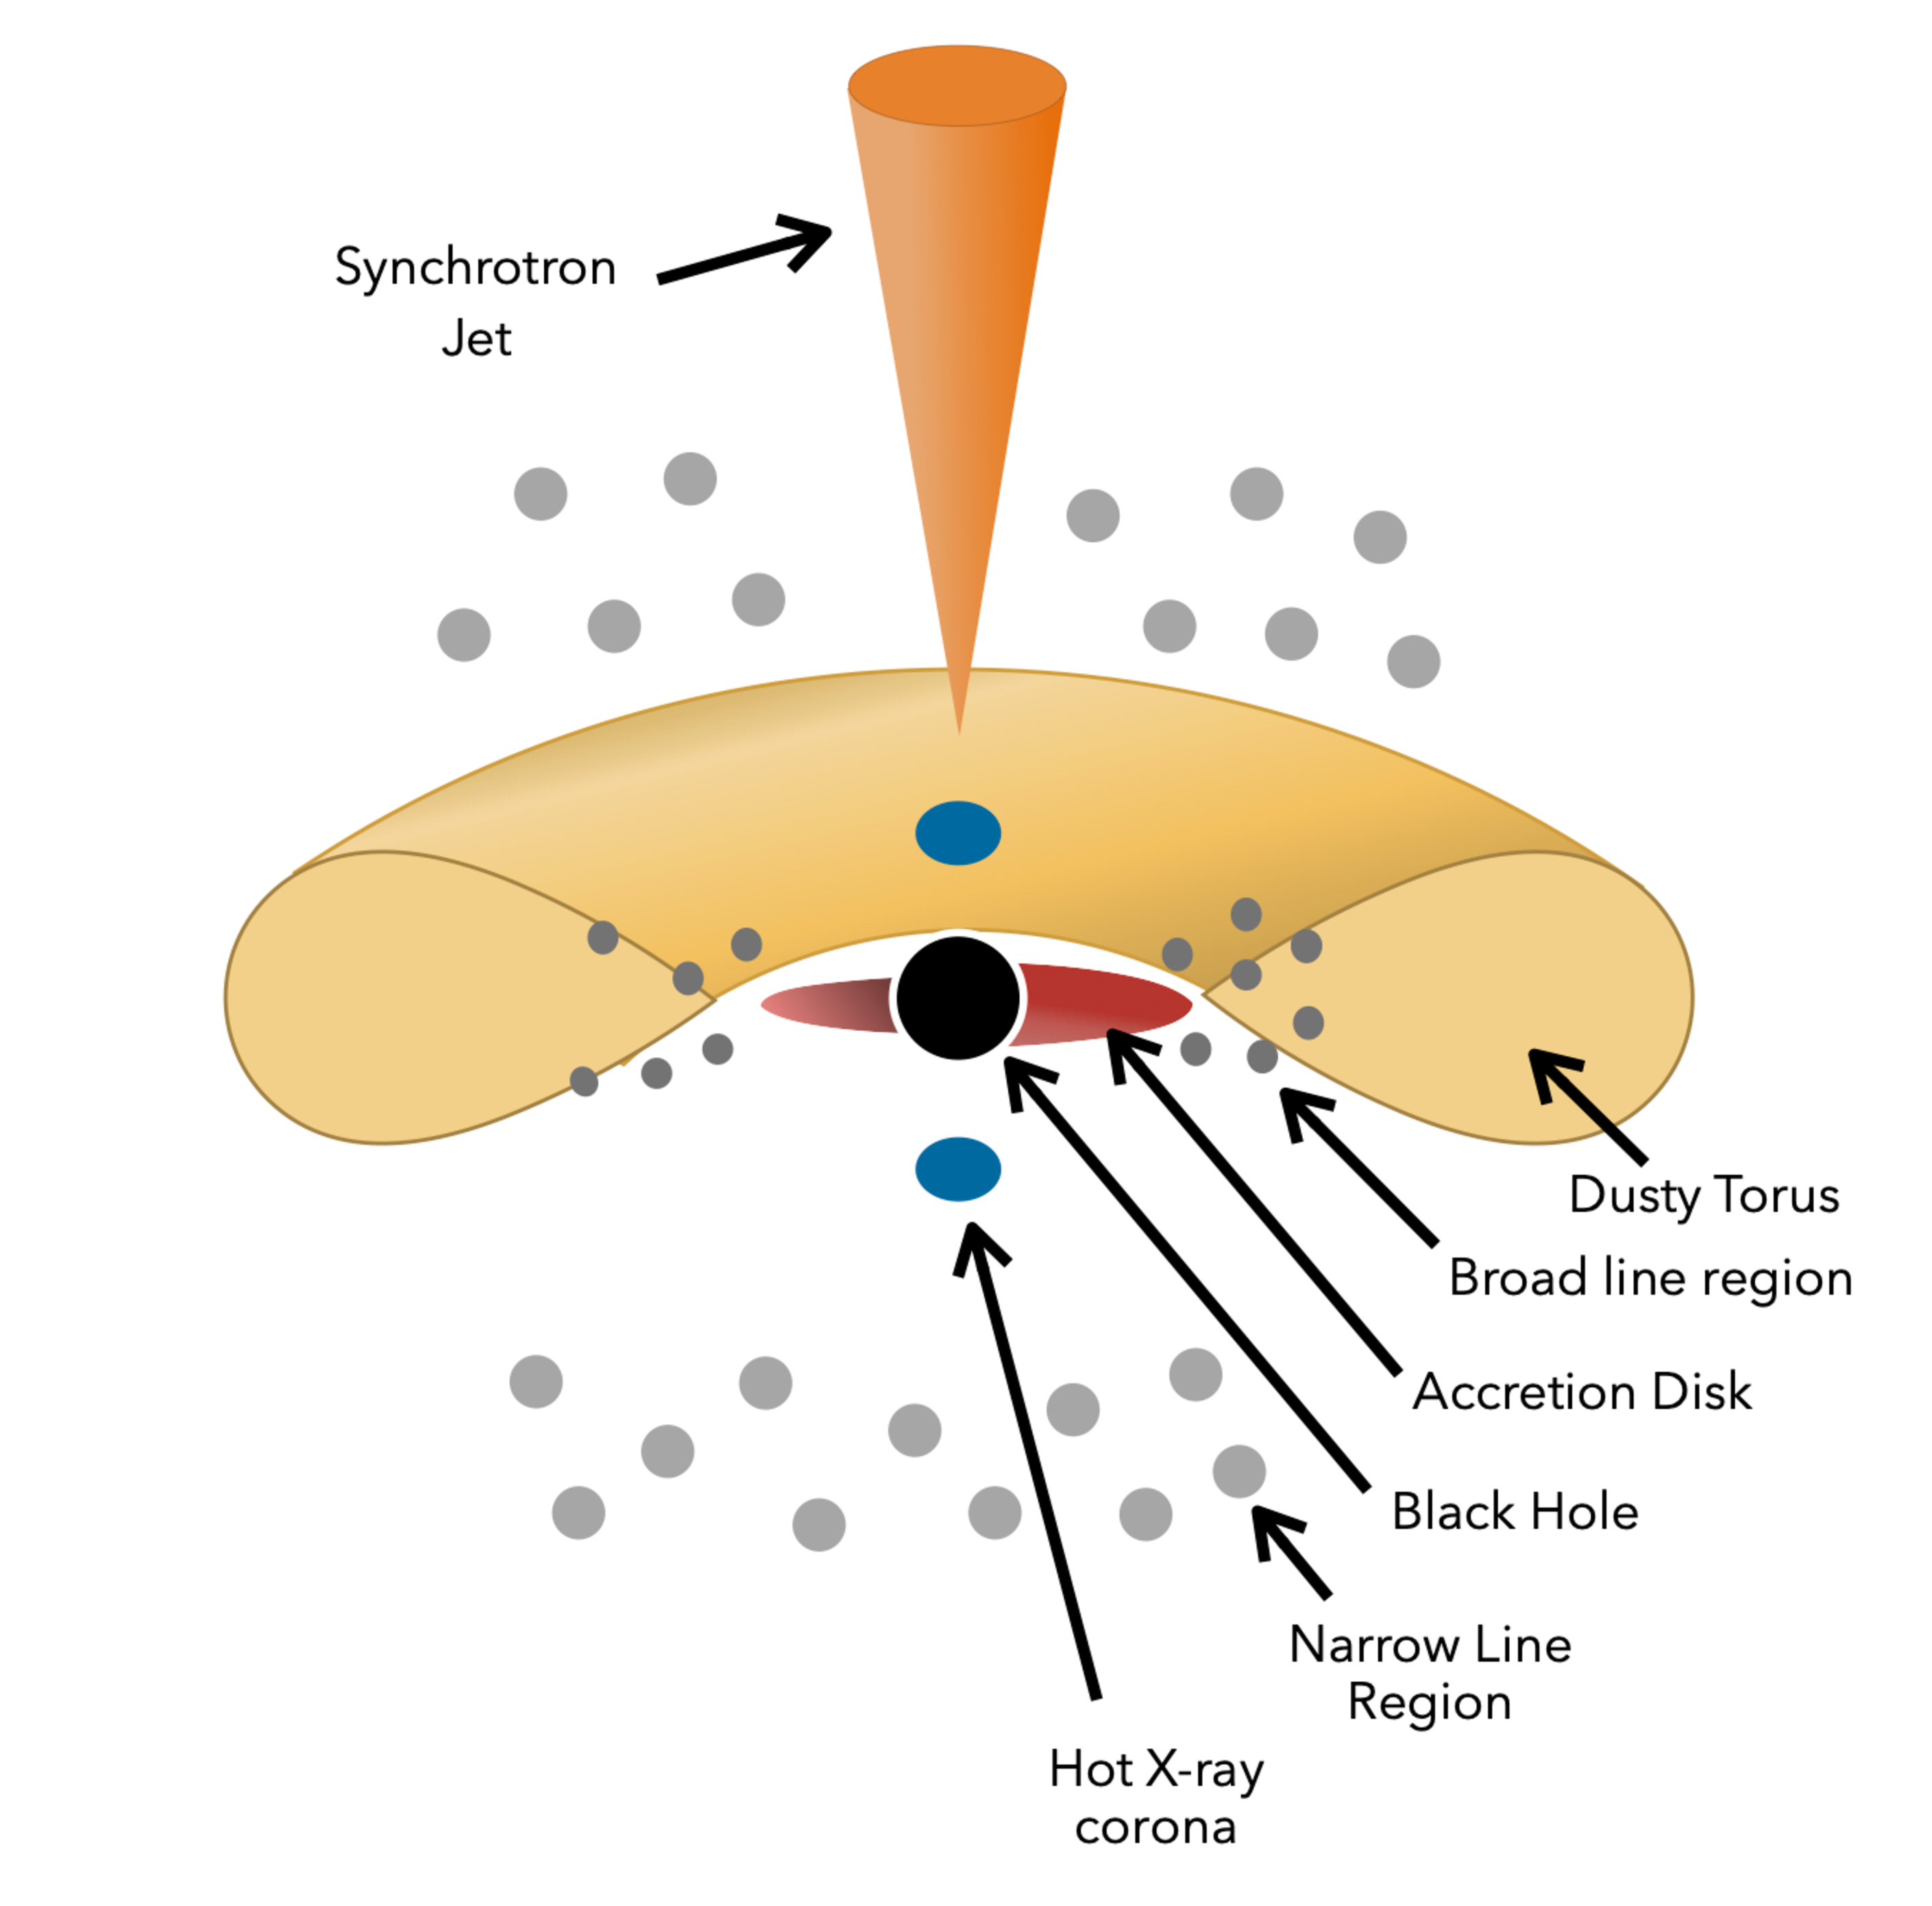
\includegraphics[width=1\textwidth]{intro_figs/AGNUnificationSteps_AGNComponents.pdf}
\caption[Components of an Active Galactic Nucleus]{Cartoon showing the various components of and AGN that affect observations.
The SMBH, accretion disk, and NSC (not shown) are of primary importance here.
Image credit: \citet{Thorne22}.}
\label{fig:agn-components}
\end{figure}



With such a high density of stars and BH in the vicinity of the SMBH, a fraction of the orbits will be embedded in the accretion disk, while others will have disk-crossing orbits.
Furthermore, AGN disks can quickly capture stars from the inclined population \citep{Fabj+20,MacLeodLin20}.
In addition to those stars initially embedded in the disk when it forms, self-gravitating AGN disks can naturally fragment and form new stars, particularly at large radii \citep{ShlosmanBegelman89, CollinZahn08}, though magnetic fields \citep{Gerling-Dunsmore+25, Tsung+25} and feedback from embedded objects \citep{HanklaJiangArmitage20} may inhibit collapse.
A hypothesis has been suggested that the disk may generate chains of hierarchical mergers between stellar-mass black holes that produce intermediate-mass black hole (IMBH) remnants \citep{McKernan+12,McKernan+14, Bartos+17, Stone+17, FordMcKernan25, Abbott+20-GW190521, LVK+25-GW231123}, much like the collisional growth model for planet formation in circumstellar disks \citep{Pollack+96}.
\Fig{fig:sbhcapture} shows a cartoon of this scenario.

\begin{figure}
\centering
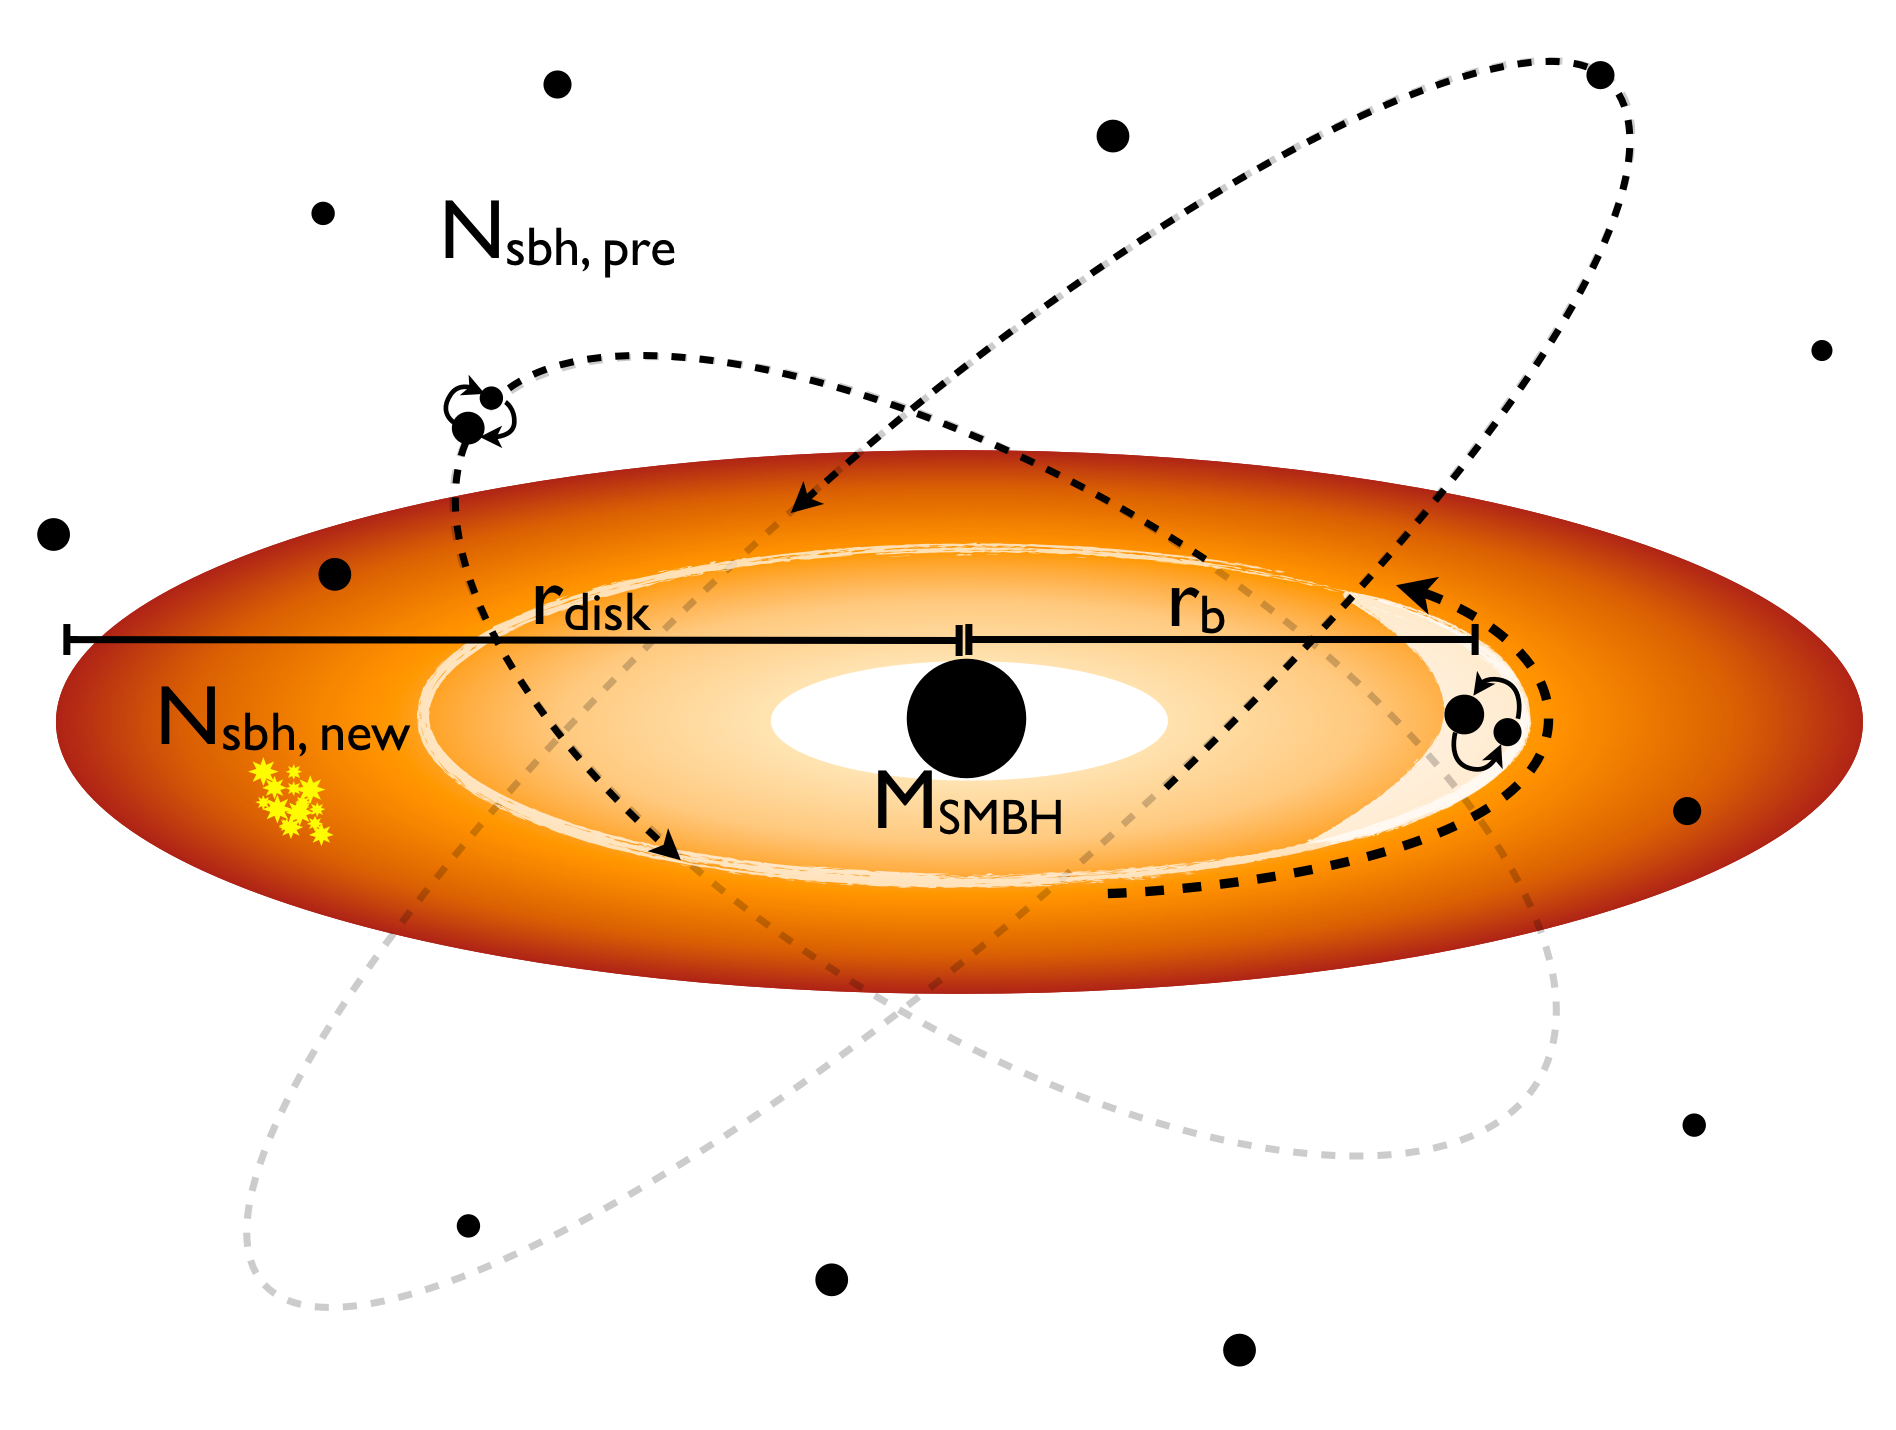
\includegraphics[width=1\textwidth]{intro_figs/sbhcapture2.png}
\caption[Interactions between an AGN disk and NSC]{Cartoon showing an AGN disk capturing BHs, forming binaries, and star formation.
Image credit: \citet{Ford+19}.}
\label{fig:sbhcapture}
\end{figure}


\subsection{The Sirens -- Multi-Messenger Probes of AGN Disks}
\subsubsection{Gravitational Waves}
Prior to 2015 the field of multi-messenger astronomy was restricted to three sources: EM radiation, cosmic rays, and neutrinos.
But on the 14th of September 2015, the first gravitational wave (GW) detection was made (called GW150914) by the Laser Interferometer Gravitational-Wave Observatory (LIGO) that was caused by the merging of two stellar mass black holes with masses $M=35_{-3}^{+5}\,\Msun$ and $30_{-4}^{+4}\,\Msun$ in the source frame \citep{GW150914}.
Two years later the first merger between two neutron stars (NS) was detected on the 17th of August 2017 \citep[GW170817,][]{nsGW170817}.
Though unknown at the time of detection, since the progenitor objects were not BHs, it was possible for the merger event to emit other forms of radiation.
The first such detection was gamma ray burst (GRB) named GRB 170817A observed by \emph{Fermi} and \emph{INTEGRAL}.
Then, an EM counterpart, named kilonova AT2017gfo, was observed in the galaxy NGC 4993 \citep{emGW170817} sparking a new age of multi-messenger astronomy.


\begin{figure}
\centering
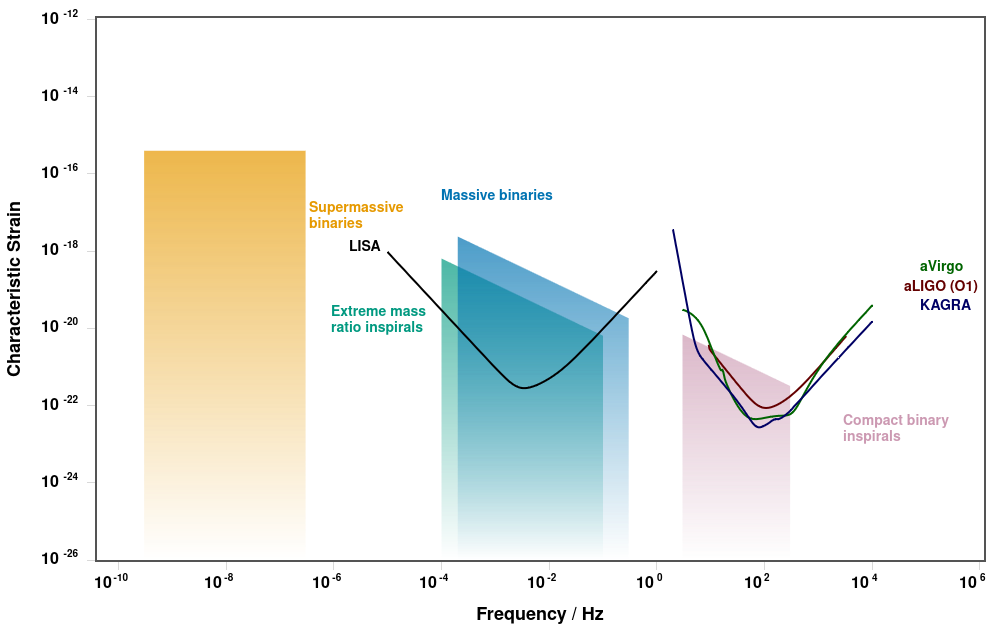
\includegraphics[width=1\linewidth]{intro_figs/gw-spectrum-detectors.png}
\caption[Gravitational wave source spectrum]{Categories of gravitational wave emitters and detector limits for LISA, aLIGO, aVirgo, and KAGRA.
Image credit: gwplotter.com \citep{Moore+15}.}
\label{fig:gwspectrum}
\end{figure}

LIGO and sister detectors Virgo and the Kamioka Gravitational Wave Detector (KAGRA) measure gravitational waves in the $\sim10-100$~Hz range that covers the final few moments of compact binary inspirals (see \Fig{fig:gwspectrum} that shows GW sources and detector limits).
In the future, the Laser Interferometer Space Antenna \citep[LISA,][]{LISA17,LISA23} will enable observations of extreme-mass ratio inspirals (EMRIs) and intermediate-mass ratio inspirals \citep[IMRIs,][]{Speri+26}.
These GW sources are comprised of single stellar mass BHs that emit long-lived GWs as they approach the event horizon of a SMBH and emit in the $\sim10^{-4}-10^{-1}$~Hz range.

Binary black hole (BBH) mergers are observed at an increasing rate as LIGO-Virgo-KAGRA (LVK) improve detector sensitivities \citep[e.g.][ see also \footnote{https://gracedb.ligo.org/superevents/public/O4/}]{Abbott+20-GW190521astro}.
Observed BBH include BH with individual masses in the expected upper mass gap ($\sim 50-120M_{\odot}$) where BHs are not expected from stellar evolution \citep{Belcynzski+16,RenzoSmith24} due to the pulsational pair instability.
A natural explanation for such BHs is via a series of hierarchical mergers that may occur in a dynamical environment, such as globular clusters \citep{Rodriguez+18}, NSC \citep{Antonini&Rasio16,Hoang+18,Fragione+19} and AGN accretion disks \citep{McKernan+12,McKernan+14,Bartos+17,StoneMetzgerHaiman17, ArcaSedda23,FordMcKernan25}.
Among hierarchical merger models, AGN are notable for both the efficiency of BBH formation as well as for retaining most post-merger products since even strong kicks from mergers correspond to small orbital perturbations in such a deep potential well.
This hypothesis is supported by the possibility that GW231123 is consistent with a merger between fourth and third generation BHs through the AGN channel \citep{Delfavero+25-GW231123}.

\subsubsection{Forming Binary Black Holes in Active Galactic Nuclear Accretion Disks}
Action of gas as a dynamical coolant and dynamical encounters drive BBH formation \citep[e.g.][]{Rowan+23,QianLiLai24,DodiciTremaine24}.
BHs embedded in AGN disks experience gas torques and can migrate \citep[e.g.][]{Syer+91,Levin07,McKernan+12}, where differential migration between BHs of different mass leads to encounters with other BH (as well as neutron stars and stars) and binary formation.
Binaries in AGN can be hardened or softened via dynamical encounters \citep[e.g.][]{Leigh+18,Samsing+20,Wang+21} or gas torques  \citep[e.g.][]{Tiede+20,Derdzinski+21,YapingLi+21}, resulting in a high rate of IMBH formation relative to other channels \citep{McKernan+12,Bellovary+16,Secunda+21,Yang+19,McKernan+20a,TagawaHaimanKocsis20,Vaccaro+24}.
Such mergers can occur at migration traps \citep[e.g.][]{Lyra+10,Sandor+11,Horn+12,Bellovary+16,Yang+19,Secunda+20}, in the bulk disk \citep[e.g.][]{Tagawa+20spin,McKernan+20a} and kicked outside the disk itself \citep{Tagawa+20b}.
However, if gap formation by IMBHs occurs, their presence may disrupt migration traps \citep{Gilbaum+25} but could also promote binary formation between nearby BHs through orbital resonances \citep{Horn+12} and at the gap edges \citep{KuchnerLecar02,Masset+06}.
The rate of BBH mergers from AGN is also expected to be significantly higher than from quiescent NSCs \citep{FordMcKernan22}.

These mergers in AGN disks should be detectable with gravitational waves \citep{McKernan+14,Bartos+17,Stone+17,Secunda+19} and could produce measurable EM counterparts from interactions with the AGN gas which would be otherwise absent for two black holes merging in the field \citep{McKernan+19,Perna+21}.

When BHs merge, we can retrieve the mass-weighted spin vector of the component BHs $\chi_i$ projected onto the binary's orbital angular momentum vector $\Lbin$ called the effective spin $\Xeff$.
This value ranges from -1 (both BH spins anti-aligned with $\Lbin$) to +1 (all vectors aligned; more about this in Ch.~\ref{sec:qXeff}, including a diagram shown in \Fig{fig:xeff-cartoon}).
The observed population of BBH mergers exhibits a bias towards $\Xeff>1$ \citep{Abbott+23-O3b}, implying they originate from formation channels that bias spin directions towards alignment with BBH orbital angular momentum.
This is not expected from gas-free hierarchical merger channels, but can occur in the AGN channel as BHs are torqued towards alignment with the gas disk over time \citep{Tagawa+20spin,Vajpeyi+22,McKernanFord24}.

Additionally, there is a possible anti-correlation observed in the mass ratio $q$ and effective spin $\Xeff$ distribution of BBH mergers \citep{Callister+21}.
This anit-correlation seems difficult to achieve in standard variants of other dynamical merger channels (e.g. globular clusters and NSC), although see \citet{Su25} for a discussion of how such an anti-correlation might arise in a dynamical triple channel.
In the isolated binary channel, \citet{Olejak+24,BanerjeeOlejak24} demonstrate the possibility of generating a $q$--$\Xeff$ anti-correlation via stable mass transfer.
In the AGN channel, an anti-correlation can arise due to several physical biases \citep{McKernan+22:q-Xeff,Santini+23, DittmannDempseyLi24}.
\citet{Vaccaro+24} show that if gas hardening is efficient in AGN, then the $q$--$\Xeff$ distribution should extend to significantly smaller values of $q$ and high $\Xeff$.
Thus, LVK O4 results can directly test gas hardening efficiency in AGN channel models, and through population studies, we can explore disk and NSC paramter space and binary formation mechanisms to give context for those GW observations.

Note that the AGN channel accounts for a still-uncertain fraction $f_{\rm AGN,BBH}$ of the observed LVK GW events.
We will learn considerably about the average properties of AGN and NSCs out to $z \sim 1$ by constraining $f_{\rm AGN, BBH}$, \emph{regardless of its actual value} (see \citealt{FordMcKernan25} for a more detailed discussion of this point).
Thus, in presenting distributions of AGN channel events in $q$--$\Xeff$ as a function of model choices, we are not claiming that AGN are responsible for all (or any) of the observed events.
Rather, we are demonstrating areas of AGN parameter space that might be ruled out by comparing with LVK O4 (O5) results that in turn hopefully allows us to constrain $f_{\rm AGN,BBH}$.




\subsubsection{Electromagnetic Waves}

As our detectors become more sensitive and the detection algorithms become more accurate, EM follow-up campaigns will become easier and more targeted.
Also, the expansion of transient surveys like the Legacy Survey through Space and Time (LSST) conducted by the Vera Rubin Telescope will allow archival searches for counterparts that could not be targeted in real time.
Yet, such a dynamic environment has the potential to produce many transient signals that must be distinguishable from one another to ensure we accurately identify counterparts to GW sources.
Among these are phenomena known as quasi-periodic oscillations (QPOs), quasi-periodic eruptions (QPEs), tidal disruption events (TDEs), changing-look AGN, supernovae (SNe) from the NSC, and anomalous flares.
These potential sources of noise must be studied to enable the search for potential EM counterparts to BBH mergers.

The first candidate EM counterpart to a gravitational wave detected binary black hole (BBH) merger was reportedly observed as a flare in AGN J124942.3+344929 by the Zwicky Transient Facility (ZTF) that was designated as ZTF19abanrhr \citep[][see \Fig{fig:counterpart-flare}]{Graham+20}.
Since the flare was inside the source volume of the gravitational wave detection GW190521 \citep{Abbott+20-GW190521} the authors suggest it could have been produced by the recoiling remnant black hole if the merger had occurred within the AGN accretion disk and experienced ram-pressure stripping of the gas bound within its Hill sphere by the disk \citep{McKernan+19}.
Using this model \citet{Graham+20} predicted a black hole mass $M\approx150\,\Msun$ which was later confirmed by the LIGO Scientific Collaboration and the Virgo Collaboration \citep{Abbott+20-GW190521}.

\begin{figure}
\centering
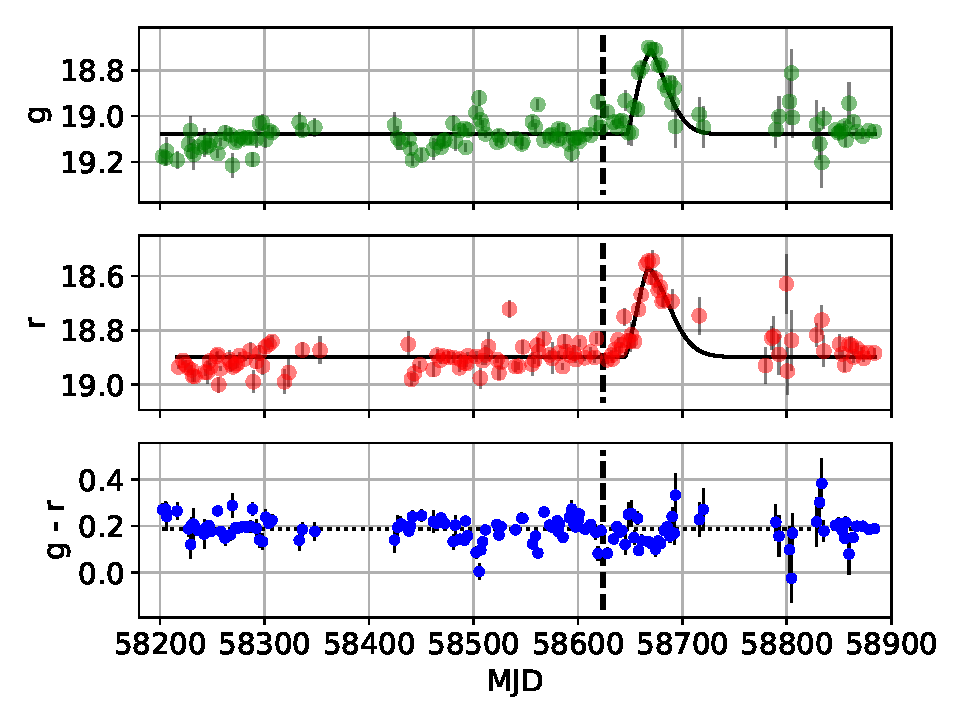
\includegraphics[width=1\textwidth]{intro_figs/counterpart-flare.pdf}
\caption[Proposed counterpart flare to GW190521]{ZTF $g$ and $r$ magnitudes and $g-r$ color for flare ZTF19abanrhr that has been proposed as an EM counterpart to GW190521 detected on the date marked by the dashed line.
Image credit: \citet{Graham+20}.}
\label{fig:counterpart-flare}
\end{figure}

They dismissed a SN as the source of the flare because it did not show any color evolution as is typical of SNe light curves \citep{Hueichapan+25}.
However, the integrated energy of the flare was $\sim10^{51}$ erg s$^{-1}$, which is conspicuously the typical energy budget of a core-collapse SN (or Type II).
A class of observed SNe are denoted as superluminous SNe (SLSNe) since their light curves peak above $\sim 10^{44}\,\text{erg s}^{-1}$ \citep{Gal-Yam12}.
One possible origin of these SLSNe is from stars that experienced extensive mass loss during their final years pre-SN \citep{Moriya+13}.
The amount of radiated energy increases with the envelope mass until the mass is similar to the ejecta mass, and the width of the light curve increases with the envelope size \citep{GinzburgBalberg12}.
If embedded SNe interact with a dense AGN disk in a similar way, their radiation may likely also be larger than their ``naked" cousins whereby the disk reprocesses much of their mechanical energy into radiation as the shock heats the disk, possibly making them observable against the bright AGN disk.
SNe in the dusty outskirts of AGN disks may have already been detected as bright optical and infrared flares \citep[e.g.][]{Assef+18}.

%We are motivated to explore the evolution of SNe embedded in an AGN disk due to the possibility that AGN flares could be EM counterparts to the gravitational wave detections from binary black hole (BBH) merger events, one particular case to underscore being GW190521 \citet{Abbott+20-GW190521}.
%While the observed flare \citep{Graham+20} did not resemble a standard SN light curve, embedded SNe could behave differently than SNe occurring in the ISM. 

%Galactic nuclei contain stars, some of which, if embedded in an active galactic nucleus (AGN) disk could detonate as embedded supernovae (SNe).
Any massive embedded stars may detonate as SNe within the disk confines, though stellar evolution in AGN disks may proceed very differently than in the interstellar medium \citep[ISM,][]{CantielloJermynLin21}.
Even in this case, SNe may yet result from stellar evolution \citep{Jermyn+21} or collisions and contribute to disk turbulence \citep{Moranchel+21}.

Whether the radiation from SNe escapes from an AGN disk is a separate matter from the mechanical breakout of the shockwave.
The non-uniform density and variable disk thickness have large impacts on a SN shock's morphological evolution in comparison to their galactic counterparts \citep{MacLowMcCray88}.
The right combination may slow down a SN shock significantly or prevent it from escaping entirely, thus depositing their kinetic energy in the disk.
These muffled SNe may not excavate the disk but could still be a contributing energy source for driving turbulence and maintaining pressure support in disks that would otherwise collapse under self-gravity \citep{Rozyczka+95,Moranchel+21}.

Characterizing light curves and color evolution from these embedded SNe is crucial for accurately distinguishing between potential transient events present in AGN disks during archival searches and live rapid-response follow-up campaigns for counterparts to gravitational wave events.
Furthermore, by understanding how SNe appear in AGN, we can rule out false positive counterparts to black hole mergers as well as constrain the rate of SNe in AGN.
Looking forward, detections of embedded SNe (or other transients in AGN disks) will allow us to constrain the composition, evolution, and dynamics of nuclear star clusters that coexist with an AGN disk, as well as to probe the disk properties.


\subsection{Primary Science Questions}

AGN are complex, dynamic systems that produce highly energetic events that impart large amounts of feedback on their environments.
It is possible that AGN disks are places to easily form and merge BBHs.
Since observing physical conditions in AGN disks and galactic nuclei in general is difficult, we can use population studies of GW detections from AGN with varying parameters to isolate parameters that reproduce the existing GW observations thereby constraining the physical conditions of the environment.
The presence of the gas provides a potential for EM counterparts to these mergers that would be impossible otherwise.
In order to accurately tie EM flares to BBH mergers, we must rule out other transients as potential sources of confusion.

\noindent To address these issues, we set out to investigate the following questions:

\begin{itemize}
\item \emph{Question 1:} What do the properties of binary black hole mergers in active galactic nucleus accretion disks reveal about the nuclear star cluster and disk properties?

\item \emph{Question 2:} What are the distinguishing characteristics of core-collapse supernovae that occur in accretion disks, and are they observable?
\end{itemize}




\subsection{Modeling Techniques}

We employ the following tools and methods to investigate the interactions between and the observational signatures of BBH mergers and SNe in AGN disks.

\subsubsection{Monte Carlo Simulations}

We use Monte Carlo simulations to explore the myriad process and vast parameter space involved with understanding how BBH form and merge in AGN disks.
Monte Carlo simulations are a numerical technique that randomly draws samples from a distribution of values that are assigned a probability of being selected.
Common probability distributions are uniform (the same probability everywhere) and Gaussian (with some characteristic mean and width), but they can be more sophisticated depending on the prior knowledge of the distribution being sampled.
Using this method, we draw random samples of parameters such as mass, orbital parameters, or spatial distributions to generate a representative subpopulation of quantities that evolve in time according to analytical expressions for physical processes.
This allows us to test different models for parameters and processes (e.g., accretion mechanism, orbital evolution, and mass functions) to compare their effects on the resulting merger population relative to each other.

The groundwork for this technique applied to mergers in AGN disks was laid out in \citet{McKernan+20a,McKernan+20b}.
The work presented details the effort to expand on it with a new code that is more robust, flexible, and user-friendly \citep{McKernan+25-mcfactsI,Cook+25,Delfavero+25-mcfactsIII,McPike+26-mcfactsIV}.

\subsubsection{Hydrodynamic Codes}

Hydrodynamics is the study of the physics of fluids.
For SNe embedded in AGN disks, the ejected material must expand into the dense disk.
Codes that solve the equations of hydrodynamics allow us to follow the strong shock interactions that occur between these two fluids.
\citet{Grishin+21} performed two-dimensional hydrodynamic simulations in the $r$-$z$ plane of SNe occurring in a flat slab of gas at the midplane and with a vertical offset, finding the shock breaks free from the disk above and below the midplane for both cases.
\citet{Moranchel+21} ran three-dimensional simulations in spherical coordinates for the upper half of the disk and find agreement that shocks from SNe at the midplane broke free from the disk.
We expand upon this work by estimating where SNe may break free from two AGN disk models using analytical expressions.
We verify these predictions with three-dimensional hydrodynamic simulations of a SN embedded in a vertically stratified shearing disk by exploring multiple radial and vertical locations in the disk with the \code{Athena} code \citep{Stone+08,StoneGardiner10}.

\subsubsection{Post-processing Radiative Transfer Methods}
Radiative transfer is one of the core tools at disposal to astronomers, since, until relatively recently, EM radiation was the sole mechanism by which to observe the Universe.
When properly considered, radiation can influence the temperature of a hydrodynamic system, so it would be best to include it as a component of the system of equations to solve for the hydrodynamic evolution.
However, solving radiation hydrodynamics in its full generality, by coupling the hydrodynamic equations with the equation of radiative transfer, is a formidable problem and computationally expensive, though some codes are making strides towards that end \citep[e.g.,][]{Jiang+14,White+23}.
An alternative is to apply post-processing radiative transfer algorithms to the output snapshots from a hydrodynamic code.

Existing codes were either proprietary \citep[\code{PHOENIX/3D},][]{Jack+09,HauschildtBaron10}, or we had difficulty modifying them to incorporate our hydrodynamic models \citep[\code{Sedona},][]{Kasen+06}.
We also looked into \code{RADMC-3D,} \citep{Dullemond+12-RADMC-3D}, which uses a Monte Carlo algorithm to solve the propagation of photon packets to converge on a temperature, but, there were concerns over whether it would converge in situations where non-thermodynamic equilibrium exist such as the AGN disk, SN ejecta, and nebular gas phases outside the disk.
We tried directly integrating the radiative transfer equation with AGN opacities, but that approach suffered from poor flux conservation.
We found instead that an implicit algorithm, the Feautrier method, afforded us greater accuracy, and developed our own code to implement this approach, that we called \ocotillo (we thank Shane Davis for suggesting this method).
\ocotillo simultaneously calculates the wavelength-dependent mean intensity, flux, and continuous opacity and applies it to the output from our SN models to retrieve integrated light curves and color evolutions.




We proceed to answer the questions posed above using these methods throughout the following chapters.

  % Introduction

%% Repeat as many chapters as you need with
% \clearpage
% \resetcounters
% \input{chapterX}

%\clearpage
%\resetcounters
%
\section{\texorpdfstring{\MakeUppercase{exploring active galactic nuclei with gravitational waves}}{exploring active galactic nuclei with gravitational waves}}
\label{sec:chapter-agnbbh}

\counterwithin{figure}{section}
\counterwithin{table}{section}

\par The model and results described in this chapter were published in the \textit{Astrophysical Journal} \citep{McKernan+25-mcfactsI}.
As such, the main text of this chapter is directly informed by the content of our publication.
To cite this chapter, please use \citet{McKernan+25-mcfactsI}.

\subsection{Motivation}

AGN are a promising source of the BBH mergers observed in gravitational waves with LVK.
Constraining the AGN channel allows us to limit AGN parameter space (disk density, size, average lifetime) and NSC parameter space.
Constraints on AGN and NSCs have implications for $\Lambda$CDM models of AGN feedback and models of AGN-driven SMBH merger and growth.
Here we present several qualitative studies of the AGN channel using a public, open-source, fast, reproducible code \code{McFACTS}\footnote{https://github.com/mcfacts/mcfacts}:Monte Carlo for AGN channel Testing \& Simulation.
We demonstrate several important features for testing the AGN channel, including:
i) growth to large mass IMBH is helped by the presence of migration traps or swamps,
ii) flat BH initial mass functions highlight hierarchical merger features in the mass spectrum,
iii) the $q$--$\Xeff$ anti-correlation is a strong test of the bias to prograde mergers in the AGN channel,
iv) spheroid encounters can drive a fraction of mergers with high in-plane spin components ($\chi_{\rm p}$),
v) a high rate of EMRIs are driven by an initial population of embedded retrograde BH, and
vi) both LVK and LISA are powerful probes of models of AGN disks and their embedded populations.


\subsection{Default Model Assumptions}
\label{sec:mcfacts-assumptions}

In the results that follow, default model parameters (also in \code{p1_model_default.ini}) are listed in Table~\ref{tab:default_model}. Unless otherwise specified, we assume a \citet[][hereafter SG]{SirkoGoodman03} disk model as interpolated from the \code{pAGN} package \citep{Gangardt+24-pAGN} around a $10^{8}\,M_{\odot}$ SMBH, spanning $[6,50000]\,\Rg$, with disk viscosity parameter $\alpha=0.01$ and lasting $0.5$ Myr. Average disk aspect ratio for this model is assumed to be $\sim 0.03$ and EMRIs are tracked within $50\,\Rg$ of the SMBH. A migration trap is assumed to live at $700\,\Rg$ (\citealt{Bellovary+16}, although see also \citealt{Grishin+23}). 

Following \citet{Generozov+18}, a NSC is assumed to fill the inner galactic nucleus out to $5$pc, with an inner number density profile $n\propto r^{-7/4}$ within $r\sim 0.25$pc and $n \propto r^{-2.5}$ outside that. The BH population of the NSC is normalized at $10^{4}$ inside the central ${\rm pc}^{3}$, matching inferences of the population in our own Galactic nucleus. The BH population mass distribution has a Pareto form with index $M^{-2}$, $M_{\rm BH, min}=10\,M_{\odot}$, $M_{\rm BH,max}=40\,M_{\odot}$. BH drawn from this distribution above $M_{\rm BH,max}$ are randomly assigned masses in a Gaussian pile-up centered on $35\,M_{\odot}$ of width $2.3\,M_{\odot}$, mimicking the observed pile-up in the LVK mass spectrum \citep{Abbott+23-massbump}. The initial BH spin distribution is assumed to be drawn from a Gaussian centered on dimensionless spin parameter $=0$ and of width $0.1$. Assuming an average scale height across the \citet{SirkoGoodman03} disk model, the fraction of BH with orbits coincident with the disk volume is calculated and the corresponding radial BH locations are generated from a distribution reflecting the user choice of NSC density.


Our default accretion rate assumptions for determining the change in mass, spin magnitude, and spin angle of each embedded black hole is that they accrete at Eddington, and must accrete $0.01$ of their own mass (while on a circular, prograde orbit) in order to have their spin aligned with the disk orbital angular momentum.
 
Our default assumption is a uniform distribution of eccentricity, i.e. sub-thermal, allowing for e.g. only partial recovery from a previous AGN episode that might have dynamically cooled these orbits. The uniform distribution is capped at some initial eccentricity value $e_{\rm max}$ to test the likely rate of relaxation from a previous AGN episode.
A full range of initial eccentricity distributions is tested in \citet{Cook+25} (presented in the next chapter).

 We assume that gas hardening of BBH follows the prescription in \citet{Baruteau11}. Our default model allows for dynamical interaction between the circularized population of BH in the AGN disk and the eccentric population (i.e. dynamics flag is on). 

Finally, we estimate the approximate merger rate corresponding to a particular simulation, by assuming a number density of AGN $n_{\rm AGN} \sim 10^{-3} \,{\rm Mpc^{-3}} \sim 10^{6} \,{\rm Gpc^{-3}}$. This yields the very useful approximation~\footnote{ Dong Lai, private communication} that $\mathcal{R}=1$ merger/AGN/Myr in these simulations is equivalent to a rate of $\mathcal{R}=1\,{\rm Gpc^{-3} yr^{-1}}$. We caution this is only an approximate rate estimate, as we are not accounting for the variation in merger rates or the distribution of merger parameters that may occur with variations in SMBH mass, NSC mass and AGN disk model. Such complications are explored in \citet{Delfavero+25-mcfactsIII}, where we attempt to simulate the AGN channel for the universe, with a distribution of galaxy properties.

\subsection{Testing Models with McFACTS}
\label{sec:mcfacts-testing}

\subsection{Testing nuclear star cluster models}
Using the default values outlined above, Fig.~\ref{fig:mf2} (left panel) shows the number of BBH mergers as a function of remnant mass.
In Fig.~\ref{fig:mf2} (left panel), the mass function of merged BH peaks between $[20,30]\,M_{\odot}$, with a secondary peak at $\sim [40,50]\,M_{\odot}$. The dominant, lower-mass peak is driven by mergers among the most numerous low mass BH in the initial mass function (IMF, $\sim [10,15]M_{\odot}+[10,15]\,M_{\odot}$). The second peak is driven by mergers between masses in the pile-up and the low masses ($\sim [35]\,M_{\odot} + [10-15]\,M_{\odot}$), since the former are the fastest migrators and the latter are the most common BH. The equivalent mean merger rate is $\mathcal{R}\sim 22.0\,{\rm Gpc}^{-3}{\rm yr}^{-1}$.

By contrast, Fig.~\ref{fig:mf2} (right panel) shows the same quantities, for the same BH minimum and maximum mass and toy-model pile-up but with $M_{\rm BH} \propto M^{-1}$. Qualitatively we can see that a flatter IMF drives more numerous and more massive mergers typically, with a longer tail to high mass and a significant number of IMBH ($>100\,M_{\odot}$) produced. The equivalent mean merger rate is $\mathcal{R}\sim 40.0\,{\rm Gpc}^{-3}{\rm yr}^{-1}$. Here, a flatter IMF reverses the magnitudes of the two peaks in Fig.~\ref{fig:mf2} (left panel), with the peak between $\sim [45,55]\,M_{\odot}$ dominating the merger spectrum. We also observe the emergence of a third peak at $\sim [65,75]\,M_{\odot}$, followed by a long hierarchical tail to higher masses. The toy model pile-up between $[35,40]\,M_{\odot}$ is relatively more prominent for a $M^{-1}$ IMF so both this feature and mergers among BH in this feature (at $[70,75]\,M_{\odot}$) are significantly more prominent than in the left panel. The new, third peak is an echo of the pile-up in the IMF yielding BH around $\sim 70\,M_{\odot}$ due to $\sim 35\,M_{\odot}+35\,M_{\odot}$ mergers since the relatively numerous massive BHs ($\sim 35\,M_{\odot}$) migrate fastest and tend to find each other more quickly. This picture is confirmed in Fig.~\ref{fig:m1m2} where we see an excess merger rate among the 1g-1g (gold) population in the right panel at $30-40$ in $M_{1}$ and indeed at ($M_{1},M_{2}$)$\sim 30-40\,M_{\odot}$ compared to the left panel. Intriguingly, there may be hints of an echo of the $35\,M_{\odot}$ peak in LVK's third observing run (O3) data at $\sim 70\,M_{\odot}$ which, if true, are suggestive of hierarchical mass mergers in a deep potential well \citep{Ignacio24}.  Observations of a relatively faint echo feature around $\sim 70\,M_{\odot}$ implies an IMF $\propto M^{[-1.5,-2]}$ for the AGN channel, but also requires a lower fraction of low mass BH to minimize intermediate features. Possibly a broken powerlaw IMF may be required as an input to AGN channel models. Or kicks may be important in segregation of generations between short-lived AGN phases. The relative positions and strengths of such peaks may be key in disentangling different BBH formation pathways in LVK data. For example, if in O4-O5, higher mass peaks are observed among $70M_{\odot}+70_{\odot}$ and $140_{\odot}+70_{\odot}$ BBH, these would be extremely suggestive of mergers retained in a very deep potential well, since such high generation and high spin mergers are very unlikely to be retained in clusters \citep[see also][]{FordMcKernan25}. The magnitude and relative sizes of such echo features in the mass spectrum will be explored more thoroughly in future work. 

\begin{figure*}
    \centering
    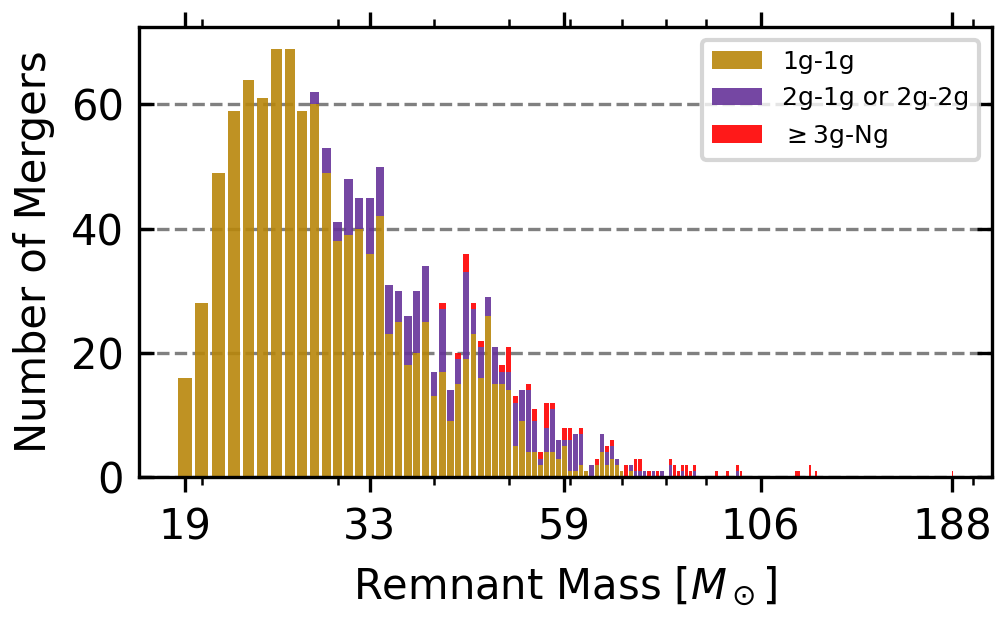
\includegraphics[width=0.5\textwidth]{ch_agnbbh_figs/default_merger_remnant_mass.png}
      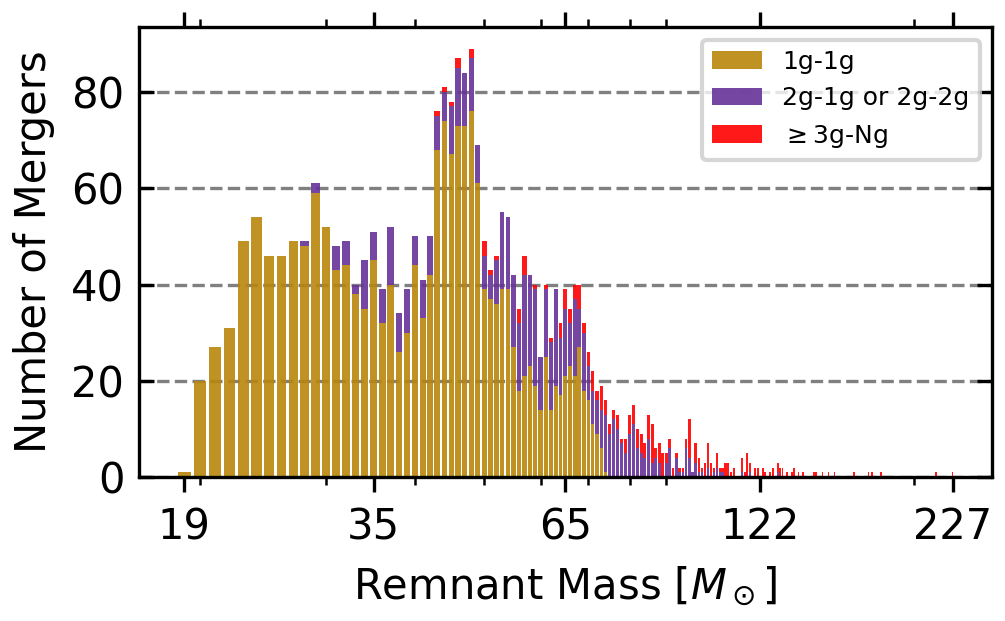
\includegraphics[width=0.5\textwidth]{ch_agnbbh_figs/p123_m1_merger_remnant_mass.png}
	\caption[Number of BBH mergers per generation of BH as a function of merged mass]{\textbf{Number of BBH mergers per generation of BH as a function of merged mass} ($M_\odot$) for different BH initial mass functions (IMFs). Left panel corresponds to a BH IMF of $M^{-2}$ with minimum $M_{\rm BH}=10\,M_{\odot}$, maximum initial mass $M_{\rm BH, max}=40\,M_{\odot}$ and simple pile-up model between $[35,40]\,M_{\odot}$ for a 0.5Myr, \citet{SirkoGoodman03} disk model around a $M_{\rm SMBH}=10^{8}\,M_{\odot}$ (see text). Gold denotes 1g-1g mergers, purple denotes 2g-mg ($m\leq 2$)and red denotes 3g-ng ($n \leq 3$) and higher, where 1g is first generation BH (not previously involved in a merger), 2g is second generation (the result of 1 merger) etc. Right panel is as left panel but with BH IMF of $M^{-1}$. Input file is \texttt{model\_choice\_old.ini} with \texttt{nsc\_imf\_bh\_powerlaw\_index = 2.(1.)} left (right), \texttt{galaxy\_num = 100} and \code{seed = 3456789018}. Equivalent merger rates correspond to $\mathcal{R}\sim 22.0(40.0) \,{\rm Gpc}^{-3} \rm {yr}^{-1}$ in left (right) panelin .
   }
    \label{fig:mf2}
\end{figure*}

\begin{figure*}
    \centering
    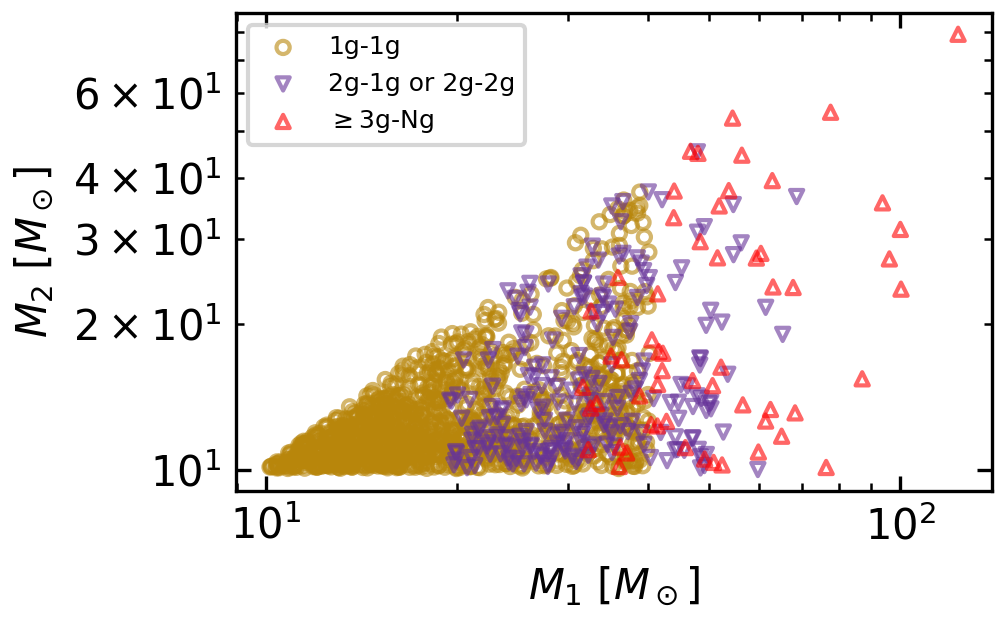
\includegraphics[width=0.5\textwidth]{ch_agnbbh_figs/default_m1m2.png}
      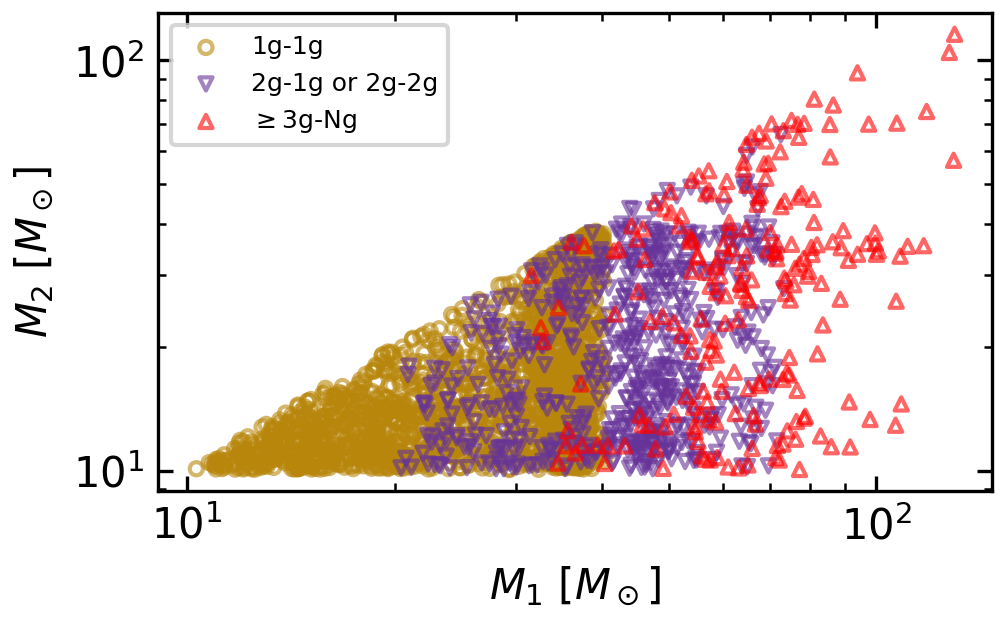
\includegraphics[width=0.5\textwidth]{ch_agnbbh_figs/p123_m1_m1m2.png}
	\caption[Distribution of merger BH masses]{Distribution of BH masses ($M_{1},M_{2}$) involved in the mergers in Fig.~\ref{fig:mf2}.
   }
    \label{fig:m1m2}
\end{figure*}

\subsection{The effect of orbital eccentricity damping}
AGN disks damp the orbital eccentricity of prograde orbiters over time \citep[e.g.][]{McKernan+12} but if the surface density increases with radius (as is the case in the inner region of the \citet{SirkoGoodman03} disk model) orbital eccentricities of retrograde orbits can be pumped \citep{Secunda+21}.

Since $t_{\rm damp} \propto h^{4}$, orbital eccentricity damping is fastest in thin parts of disk models ( e.g. $\sim [10^{2},10^{4}]\,\Rg$ in \citealt{SirkoGoodman03}). Therefore we expect BH orbits to circularize fastest in the thinnest parts of the disk. Since BBH formation is predominantly drawn from the population that have already circularized, we expect the BBH population to tend to form in the thinner parts of the disk model first.
 
If we assume an initially thermal distribution of orbital eccentricities, we expect an orbital distribution function 
\begin{equation}
    f(e){de} = 2e \;{de}
\end{equation}
such that the median orbital eccentricity is $e \sim 1/\sqrt{2} \sim 0.7$ and there is a uniform probability distribution of $e^{2}$. For initially thermal eccentricity distributions, we draw from a uniform distribution [0,1] to obtain $e^{2}$ at $t=0$. However, such a distribution is the limiting case where orbits have had sufficient time to relax and will only apply where there is a very long interval between AGN episodes. Instead, for our default case, which involves a short (0.5Myr) AGN lifetime, we introduce a maximum initial eccentricity ($e_{\rm max}$), capping the uniform distribution, corresponding to a relatively short period of relaxation between AGN episodes.

We expect new BBH to form mostly from the circularized population. The subsequent migration of such BBH either inwards or outwards, away from this disk region, will make dynamical encounters with eccentric orbiters more likely. Such encounters will be capable of either hardening, softening/ionizing the BBH, depending on the details of the encounter \citep[e.g.][]{Leigh+18,WangZhuLin24}. Note also $a \sim 10^{3}\,\Rg$ is a plausible location for a migration trap \citep{Bellovary+16} in such a disk, although \citet{Grishin+23} suggest that such traps can occur at radii $\times 3-5$ further out in the disk.

\begin{figure*}
    \centering
    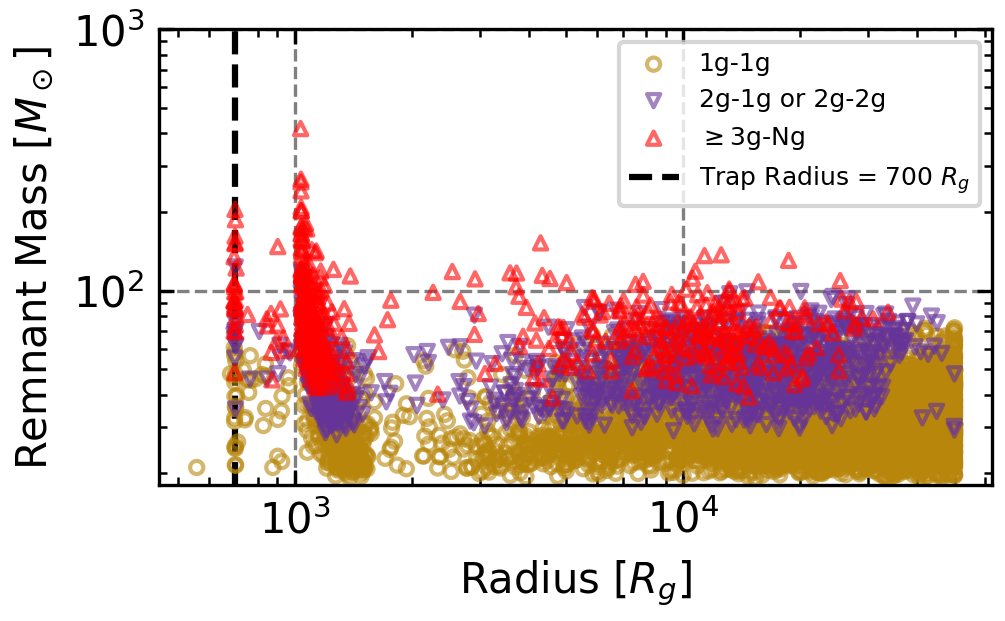
\includegraphics[width=0.5\textwidth]{ch_agnbbh_figs/p123_circ_merger_mass_v_radius.png}
      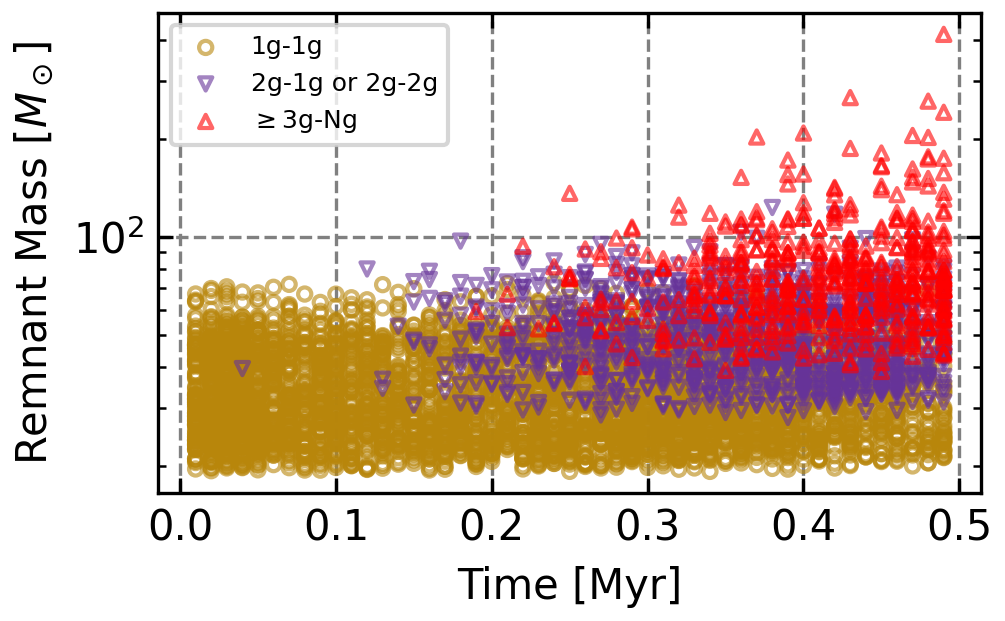
\includegraphics[width=0.5\textwidth]{ch_agnbbh_figs/p123_circ_time_of_merger.png}
	\caption[BBH merger mass as a function of disk radius and time]{\textbf{BBH merger mass as a function of disk radius (left panel) and time (right panel).} All BH are assumed initially circularized and no dynamical encounters occur. Input file is \texttt{model\_choice\_old.ini} with \texttt{flag\_orb\_ecc\_damping = 0}, \texttt{flag\_dynamic\_enc = 0}, \texttt{nsc\_spheroid\_normalization = 0.0}, \texttt{galaxy\_num = 100} and \texttt{seed = 3456789018}. Equivalent merger rate is ${\mathcal{R}} \sim 95.4\, {\rm Gpc}^{-3} {\rm yr}^{-1}.$
   }
    \label{fig:circ}
\end{figure*}





Fig.~\ref{fig:circ} shows the BBH merger masses as a function of disk radius (left panel) and time (right panel) for the setup as in Fig.~\ref{fig:mf2}, except all the BH are assumed to be initially circularized and we do not allow dynamical interactions. Feedback is on, so migration develops an outward component in the outer disk (driving a small pile-up near the outer disk edge). The equivalent merger rate is very high $\mathcal{R} \sim 95.4\,{\rm Gpc}^{-3} {\rm yr}^{-1}$ as BBH mergers start straightaway ($t=0$, right panel) and high generation mergers (2g,3g) quickly appear in $<0.1$ Myr. There is a divergence in the mass distribution of mergers in the right panel with IMBH-building mergers ($>100M_{\odot}$) starting in the first $\sim 0.2$ Myr, and growing larger over time. These  IMBH mergers occur preferentially at both the migration trap \citep{Bellovary+16}, and the migration swamp in front of the trap around $\sim 10^{3}\Rg$, where the Paardekooper migration torque drops by $\sim 30\%$ for $M_{\rm SMBH} \sim 10^{8}M_{\odot}$, leading to a pile-up at this region (see e.g. Fig.2 in \citep{Grishin+23} for an approximate illustration). The bulk of mergers are at lower mass, which was also the pattern we found in \citet{McKernan+20a} where we assumed all the BH are on circularized orbits at $t=0$. 

The largest mass IMBH occur at or near the migration trap or at the disk outer boundary. Some IMBH-producing mergers (up to $\sim 150\,M_{\odot}$) occur far from the trap, in regions of the disk where the size of the BBH Hill sphere radius is large. 

\begin{figure*}
    \centering
    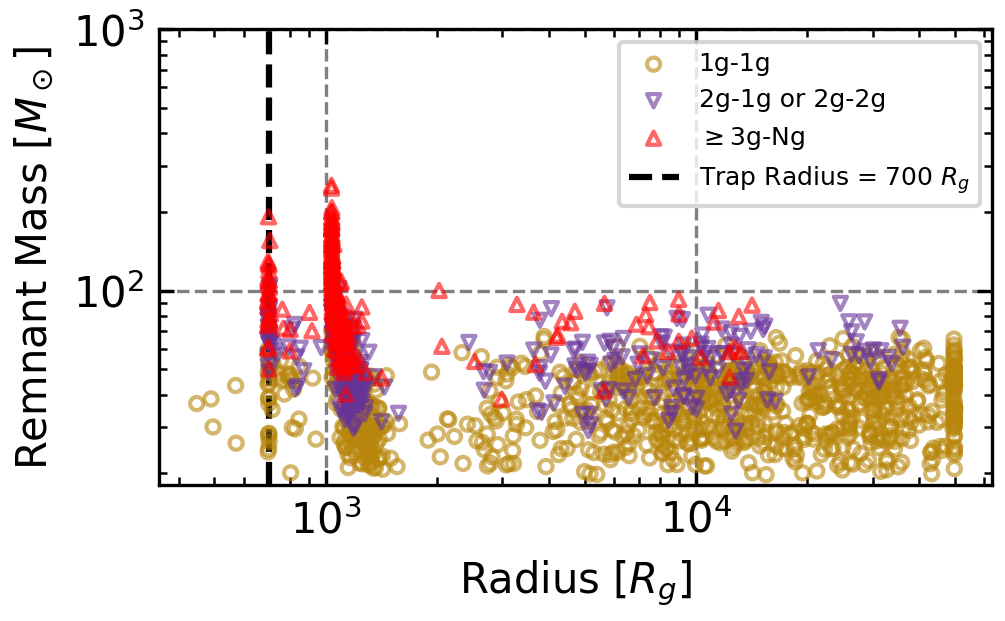
\includegraphics[width=0.5\textwidth]{ch_agnbbh_figs/p123_ec9_merger_mass_v_radius.png}
      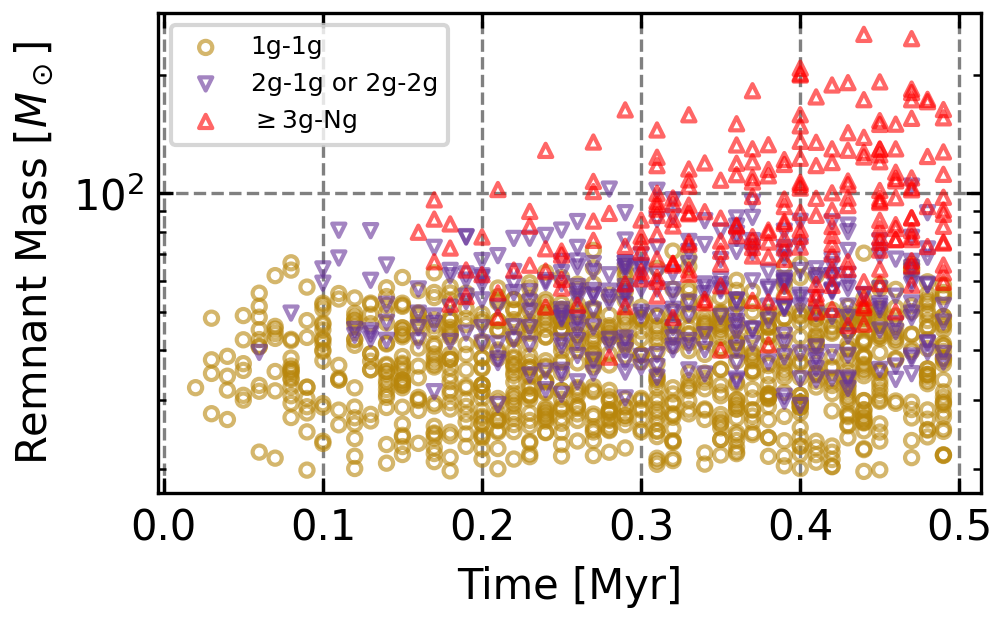
\includegraphics[width=0.5\textwidth]{ch_agnbbh_figs/p123_ec9_time_of_merger.png}
	\caption[BBH merger mass for e=[0.0,0.9]]{\textbf{BBH merger mass for e=[0.0,0.9]}As Fig.~\ref{fig:circ} except all BH are assumed to be drawn from an initial uniform distribution of orbital eccentricities between [$0.0,0.9$] and no dynamical encounters occur. Input file is as Fig.~\ref{fig:circ}, except \texttt{flag\_orb\_ecc\_damping = 1} and \texttt{disk\_bh\_orb\_ecc\_max\_init = 0.9}. Equivalent merger rate is ${\mathcal{R}} \sim 26.8 \,{\rm Gpc}^{-3} {\rm yr}^{-1}.$
   }
    \label{fig:ecc}
\end{figure*}

\begin{figure*}
    \centering
    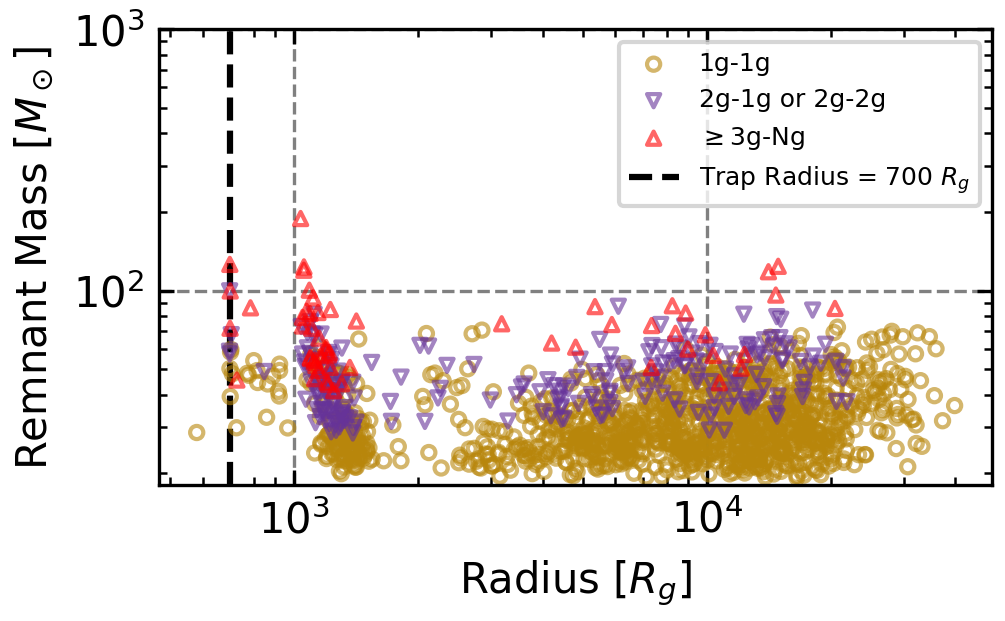
\includegraphics[width=0.5\textwidth]{ch_agnbbh_figs/default_merger_mass_v_radius.png}
      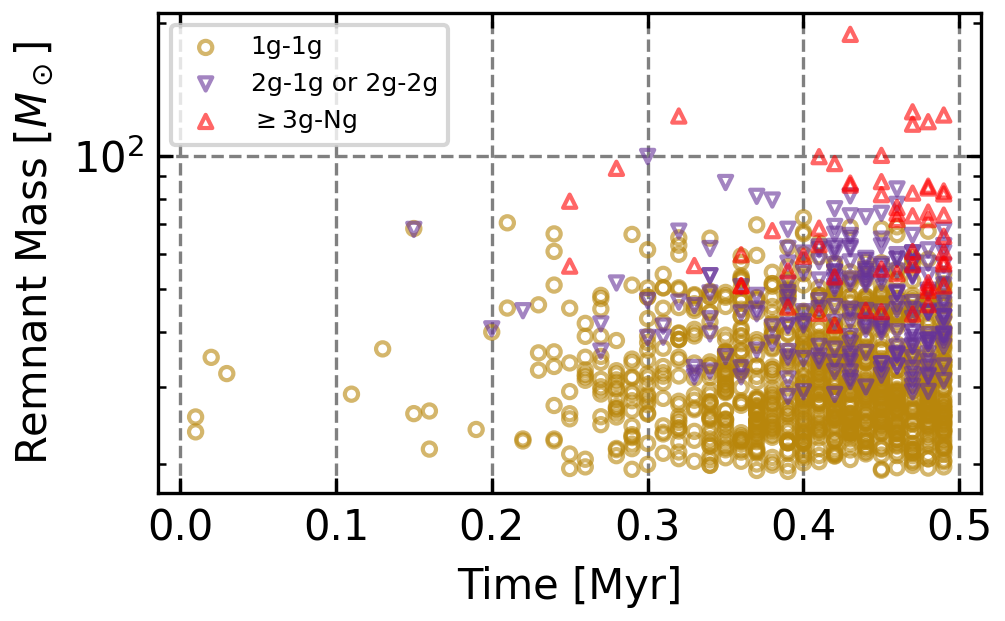
\includegraphics[width=0.5\textwidth]{ch_agnbbh_figs/default_time_of_merger.png}
	\caption[BBH merger mass for e=[0.0,0.3]]{\textbf{BBH merger mass for e=[0.0,0.3]}As Fig.~\ref{fig:ecc} except all BH are assumed to be drawn from an initial uniform distribution of orbital eccentricities between [$0.0,0.3$] and dynamical encounters are allowed. Input file is \texttt{model\_choice\_old.ini} with \texttt{flag\_orb\_ecc\_damping = 1}, \texttt{flag\_dynamic\_enc = 1}, \texttt{nsc\_spheroid\_normalization = 1.0}, \texttt{disk\_bh\_orb\_ecc\_max\_init = 0.3}, \texttt{galaxy\_num = 100} and \texttt{seed = 3456789018}. Equivalent merger rate is ${\mathcal{R}} \sim 22.0 \,{\rm Gpc}^{-3} {\rm yr}^{-1}.$
   }
    \label{fig:dyn-ecc}
\end{figure*}

\begin{figure*}
    \centering
    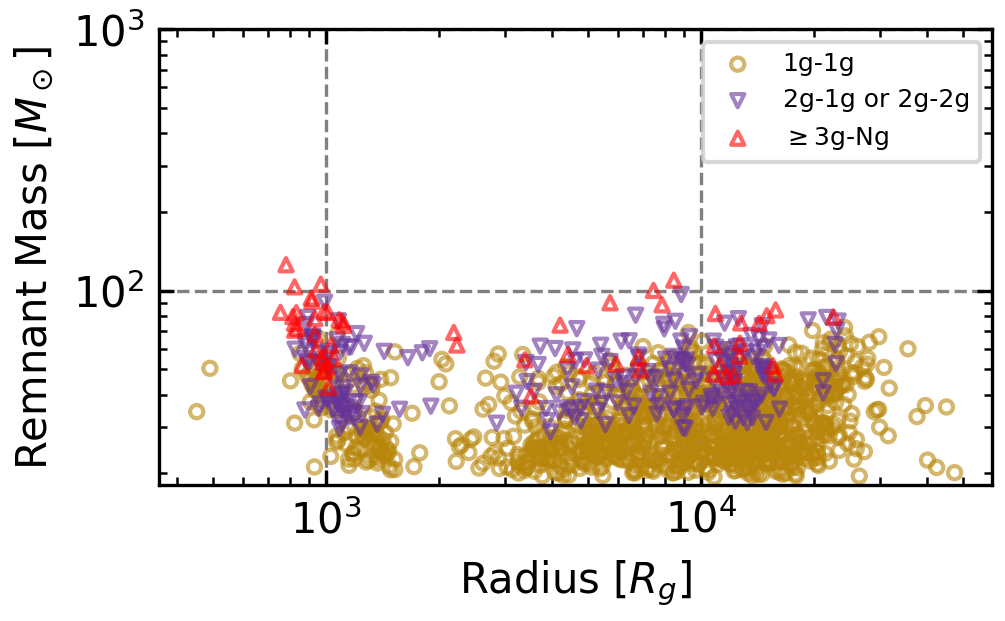
\includegraphics[width=0.5\textwidth]{ch_agnbbh_figs/jm17_m_rad_vf.png}
      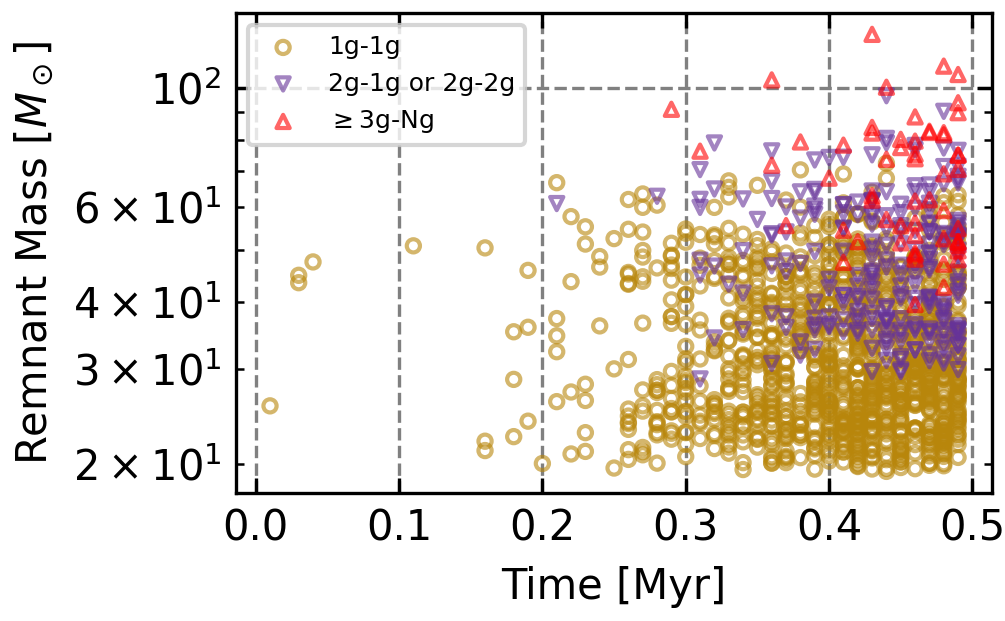
\includegraphics[width=0.5\textwidth]{ch_agnbbh_figs/jm17_time_vf.png}
	\caption[Jimenez \& Masset torque prescription]{\textbf{Jimenez \& Masset torque prescription}As Fig.~\ref{fig:dyn-ecc}, except \texttt{torque\_prescription = jimenez\_masset}. Equivalent merger rate is ${\mathcal{R}} \sim 21.2\ {\rm Gpc}^{-3} {\rm yr}^{-1}$.
   }
    \label{fig:jm}
\end{figure*}


By contrast, Fig.~\ref{fig:ecc} shows what happens if we assume an initially eccentric population (\code{flag_eccentricity_damping = 1} with a uniform eccentricity distribution), with maximum initial eccentricity = 0.9, with otherwise identical input parameters as in Fig.~\ref{fig:circ}. The merger rate drops dramatically to $\mathcal{R}\sim 26.8\, {\rm Gpc}^{-3}{\rm yr}^{-1}$ as a delay time ($\sim 0.03$ Myr) is introduced since it takes time for gas damping to begin building up the circularized BH population. This population will also preferentially occur at thinner regions of the AGN disk, so the migration swamp/trap region remains important but fewer (less massive) IMBH are now produced. 


\subsection{Testing dynamics}
Among a disk BH population where dynamics is ignored, BBHs will tend to form in regions where there is crowding (e.g. near migration traps), as in Fig.~\ref{fig:ecc}. However, things can change once we allow dynamical interactions to occur.

First, we introduce interactions between the embedded BH in the disk. Circularized BH are dynamically heated by close encounters with the eccentric population. This introduces an additional delay time ($\sim 0.3$Myr, excluding a handful of very close initial BH) before BBH can merge in addition to the gas circularization delay time seen in Fig.~\ref{fig:ecc}. The average rate of dynamical encounters among an eccentric BH population is highest in the inner disk and so the circularized population build-up near the migration trap/swamp is inhibited initially, leading to a delay in higher generation mergers. This is clear from Fig.~\ref{fig:dyn-ecc}
 where we assume $e_{\rm max}=0.3$ and the BH populations within the disk (eccentric and circularized) are allowed to interact with each other. Dynamical destruction of inner disk BBH leads to a delay in 3g-ng mergers, which first appear after $\sim 0.4$Myr vs $\sim 0.2$Myr in Fig.\ref{fig:ecc}). As we increase $e_{\rm max}$, the delay-time increases and the AGN needs to run for longer to drive a higher merger rate. Fig.~\ref{fig:jm} shows the effect of choosing a different torque prescription but all else as in Fig.~\ref{fig:dyn-ecc}. The \citet{JimenezMassset17} prescription leads to a lower torque magnitude by $\sim 30\%$ across the outer disk, delaying mergers and inhibiting higher generation mergers for an AGN of the same lifetime (again see Fig.2 of \citep{Grishin+23} for an approximate illustration).

\begin{figure}
    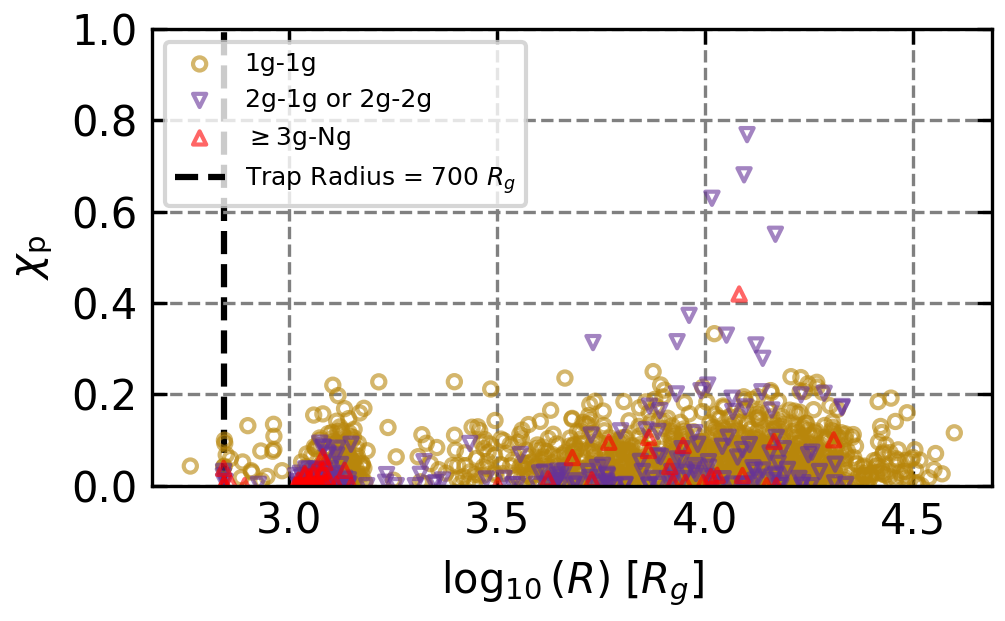
\includegraphics[width=0.5\textwidth]{ch_agnbbh_figs/default_r_chi_p.png}
    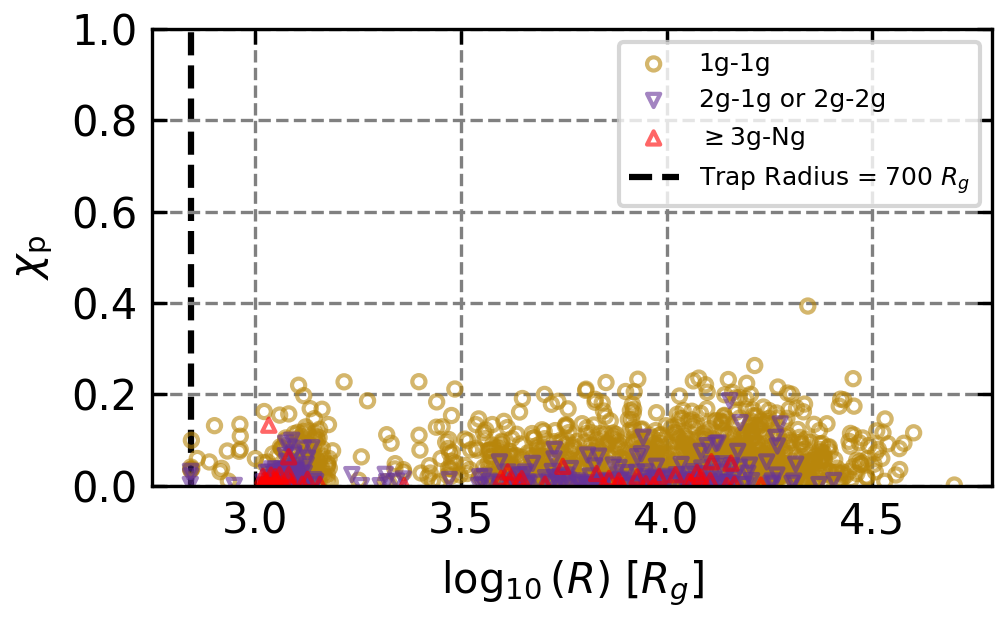
\includegraphics[width=0.5\textwidth]{ch_agnbbh_figs/p123_sphoff_r_chi_p.png}
	\caption[In-plane spin for BBH mergers as a function of disk radius]{\textbf{$\chi_{\rm p}$ for BBH mergers as a function of disk radius} where spheroid encounters are on (top panel) and spheroid encounters are off (bottom panel). Input file and parameters (top panel) are as in Fig.~\ref{fig:dyn-ecc}, and in bottom panel except \texttt{nsc\_spheroid\_normalization = 0.0}. Equivalent merger rate is ${\mathcal{R}} \sim 22.0(22.7) \,{\rm Gpc}^{-3} {\rm yr}^{-1}$ top (bottom) panel.
   }
    \label{fig:chi_p}
\end{figure}


\begin{figure}
    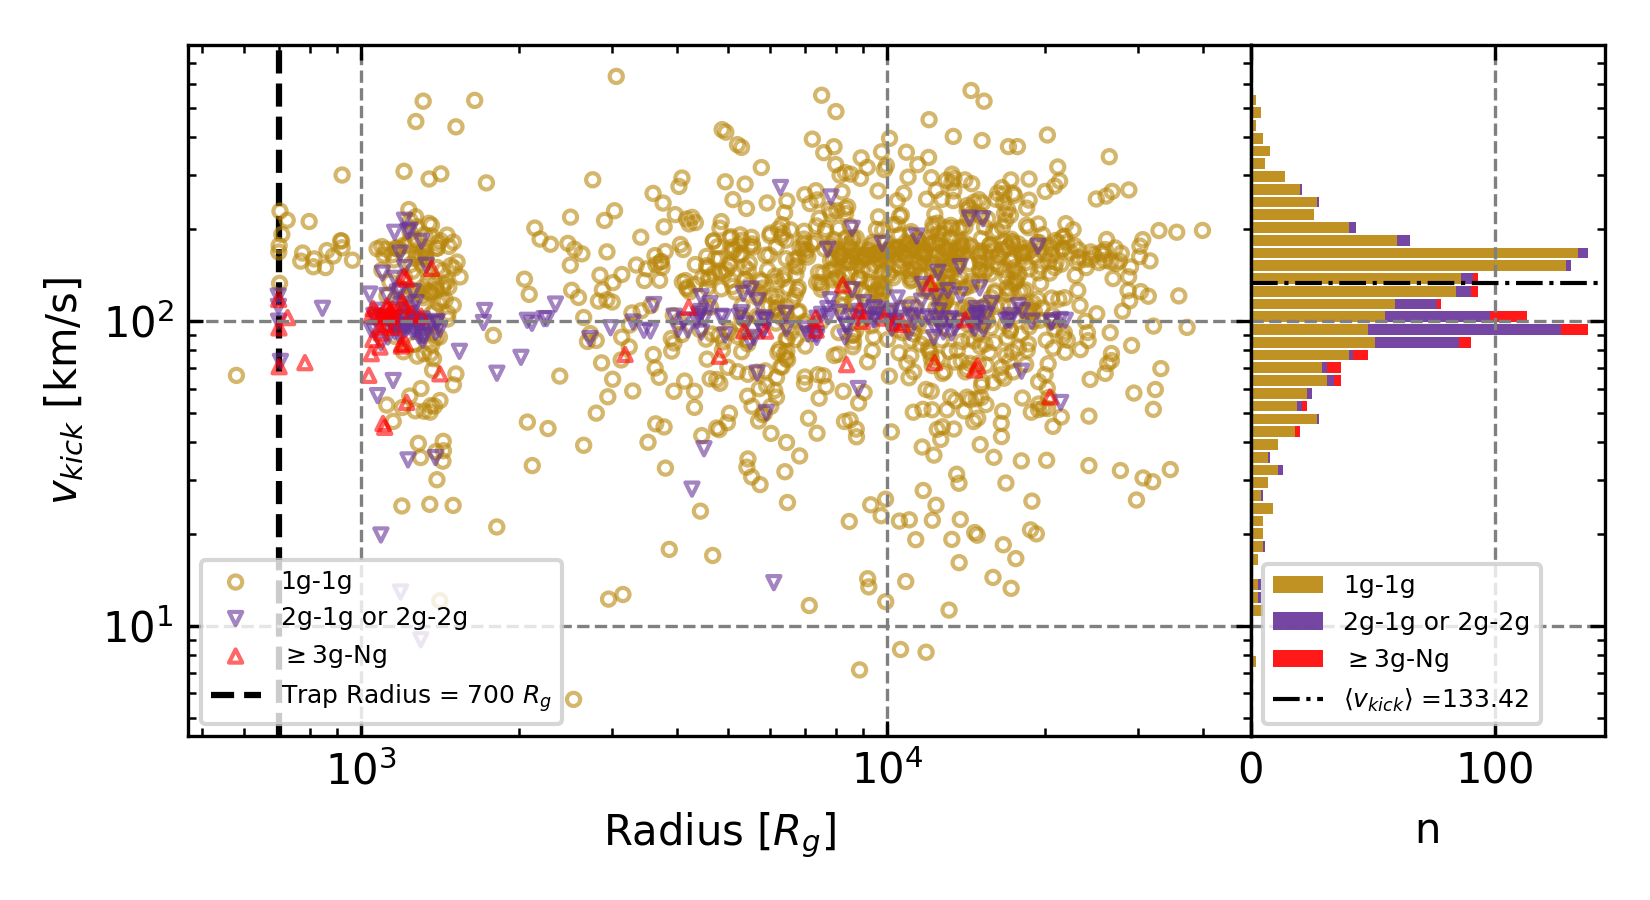
\includegraphics[width=0.5\textwidth]{ch_agnbbh_figs/default_v_kick_vs_radius.png}
	\caption[Velocity kicks vs. radius]{\textbf{Velocity kicks vs. radius.} (\emph{Left panel:})  Velocity kicks as a function of disk radius and generation associated with mergers for the model in Fig.~\ref{fig:mf2}(a). (\emph{Right panel:}) Number and generation of mergers as a function of kick velocity. Dash-dot line corresponds to mean kick velocity of $\sim 133{\rm km/s}$.
    }
    \label{fig:v_kick}
\end{figure}
Dynamically we also introduce encounters between the spheroid NSC population and the embedded BBH population in the disk. Spheroid encounter rates are highest in the inner disk, but with disk dynamics on, the overall effect on the merger rate is small (few $\%$ change). 
Spheroid encounters have a significant effect in generating a in-plane spin component ($\chi_{\rm p}$). Conservation of orbital angular momentum in moderately close interactions between disk BBH and spheroid stars will pop BBH out of the AGN disk with a new orbital angular momentum ($L_{\rm BBH}$) orientation, but individual BH spin alignments do not change, yielding a significant spin component in the plane of $L_{\rm BBH}$ \citep{Tagawa+20spin,Samsing+22,McKernanFord24}. Fig.~\ref{fig:chi_p} shows $\chi_{\rm p}$ as a function of BBH merger location in the disk with spheroid encounters on/off (left/right panel respectively) (\code{nsc_spheroid_normalization=1/0}). The highest values of $\chi_{\rm p}$ are overwhelmingly driven by higher generation (higher mass) mergers. Higher mass BBH have a larger cross-section for spheroid encounters (larger $R_\mathrm{H}$), but higher mass makes them harder to ionize via spheroid stellar encounters. This feature of the AGN channel should be directly testable in O4 by LVK.

Fig.~\ref{fig:v_kick} shows the distribution of merger kick velocities as a function of disk radius, calculated from eqn.~\ref{eq:v_kick}. First generation BH mergers (in gold) peak strongly around $\sim 200{\rm km/s}$ as we expect \citep{Varma+22}. However, higher generation BH have smaller kick magnitudes ($\sim 100{\rm km/s}$) with this prescription. We caution that this is an \emph{underestimate} of the kicks to be expected among higher generation mergers. In particular, including the relativistic evolution of the BBH allows for much higher values of the merger kick (up to $\sim 2000{\rm km/s}$) among the higher generation mergers. This will be very important for potential mass segregation between AGN phases \citep[e.g.][]{Gilbaum+25} (see also Ray et al. 2026, in prep.).

\subsection{The $q$--$\Xeff$ anti-correlation}
\label{sec:qXeff-agnbbh}
LVK observations suggest an intruiging anti-correlation between the BBH mass ratio ($q$) and the effective spin ($\Xeff$) of mergers \citep{Callister21}. The anti-correlation is consistent with greater alignment between spin and BBH orbital angular momentum for the primary BH component ($\chi_{1}$) when BBH masses are less equal. The only reason for such a anti-correlation to arise in a dynamical channel is if there is a bias towards alignment of the primary BH spin with the BBH orbital angular momentum. AGN disks can naturally provide such a bias \citep[e.g.][]{McKernan+22:q-Xeff, Santini+23}. This bias alone (via spin-up and spin torquing) is insufficient however; a bias \emph{against} retrograde BBH mergers is also required. In the AGN channel, such a bias might occur because: (i) Retrograde disk BBH are flipped to prograde over time due to gas accretion \citep{DittmannJermynCantiello23} or, (ii) retrograde BBH experience orbital eccentricity pumping \citep{Calcino+23}, so retrograde BBH should spend more time at wider separations than prograde BBH with similar semi-major axes around their center of mass \citep{WangZhuLin24}, or (iii) spheroid encounters with in-plane retrograde BBH will drive the BBH away from retrograde \citep{Samsing+22} and gas torquing tends to drive the BBH towards $\Xeff>0$. 

\begin{figure*}
    \centering
    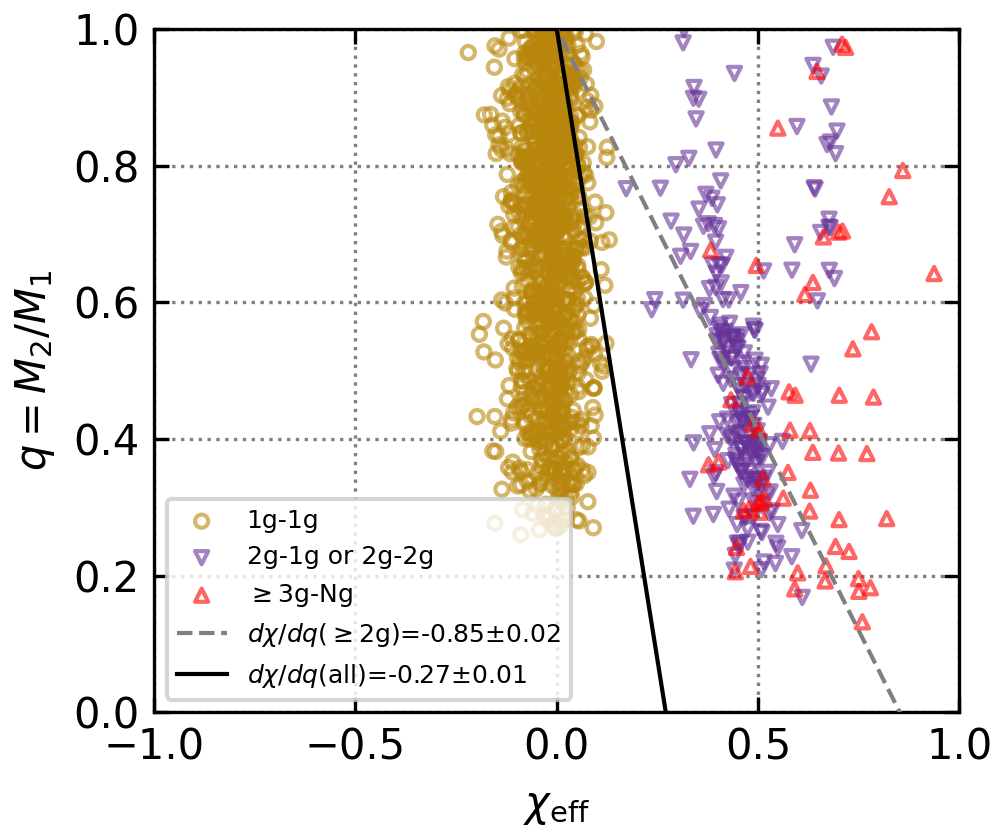
\includegraphics[width=0.5\textwidth]{ch_agnbbh_figs/default_q_chi_eff.png}
    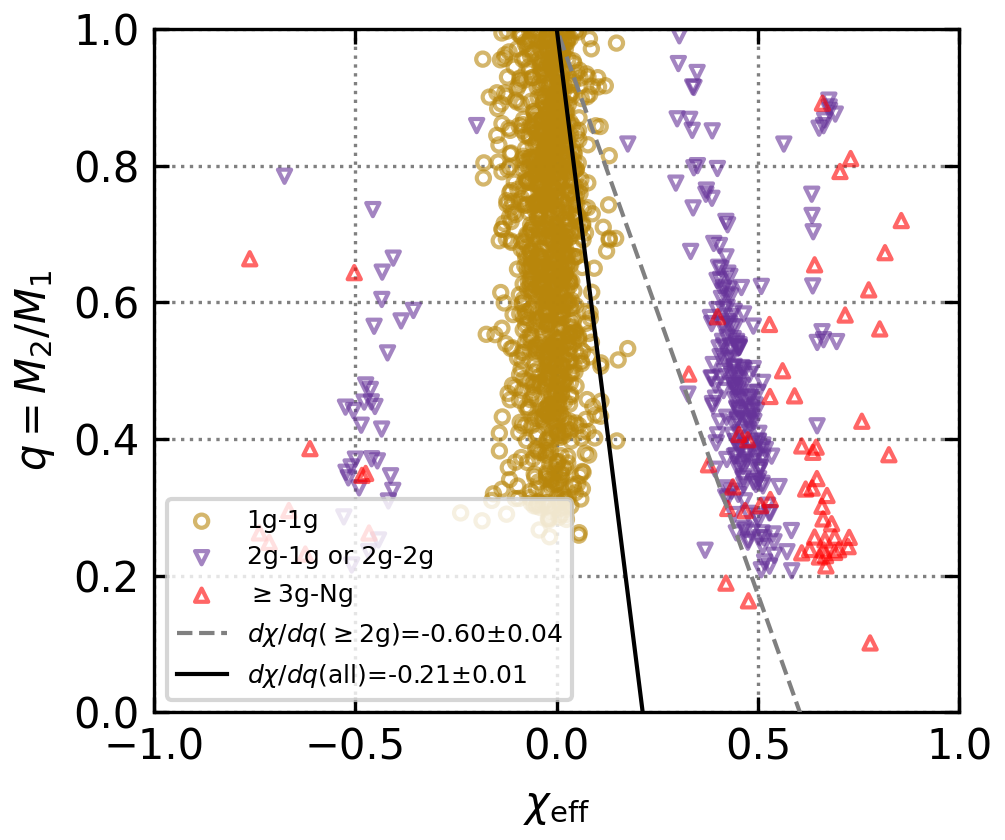
\includegraphics[width=0.5\textwidth]{ch_agnbbh_figs/p123_ret1_q_chi_eff.png}
	\caption[$q$ vs. $\Xeff$]{\textbf{Mass ratio ($q$) distribution as a function of $\Xeff$.} Left panel assumes all BBH are biased to form prograde  and right panel assumes $10\%$ form retrograde. Input file is \texttt{model\_choice\_old.ini} as for Fig.~\ref{fig:dyn-ecc} left panel and in the right panel we assume \texttt{fraction\_bin\_retro=0.1}.  Equivalent merger rates are ${\mathcal{R}} \sim 22.0(22.2) {\rm Gpc}^{-3} {\rm yr}^{-1}.$
   }
    \label{fig:qX}
\end{figure*}

\begin{figure*}
    \centering
    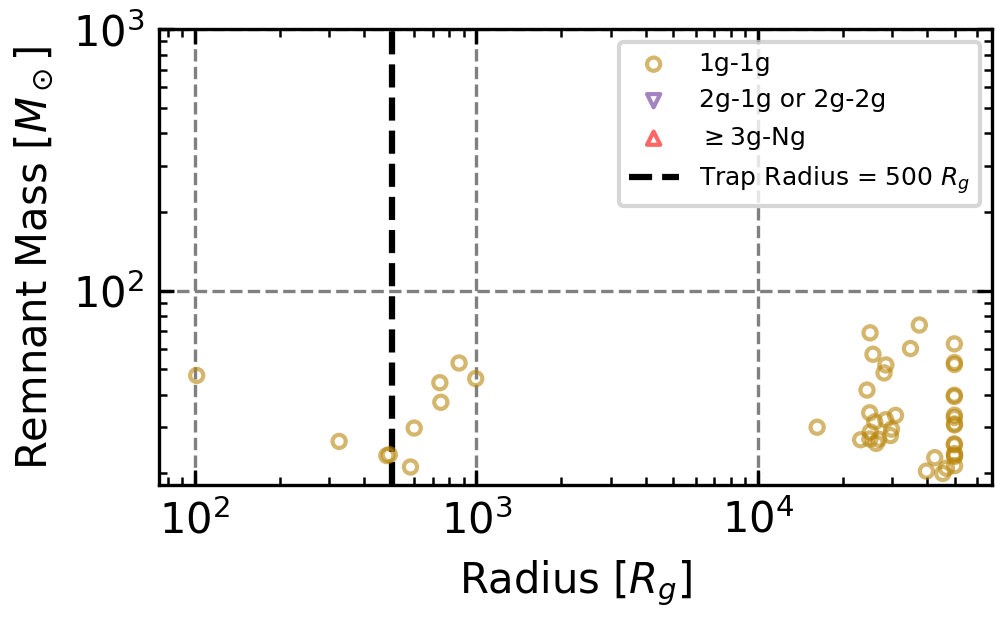
\includegraphics[width=0.5\textwidth]{ch_agnbbh_figs/p123_tqm_merger_mass_v_radius.png}
      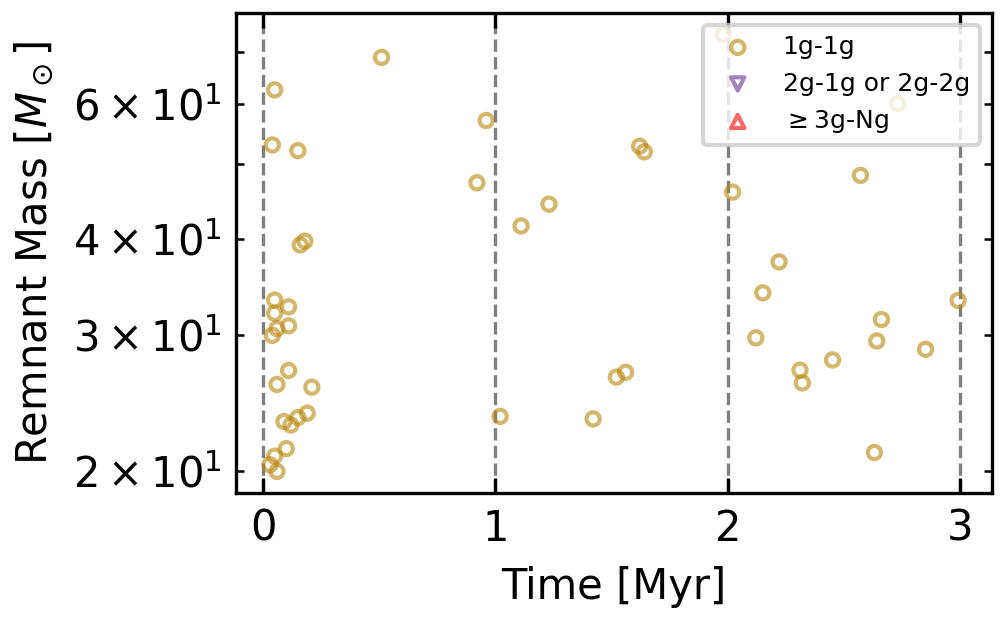
\includegraphics[width=0.5\textwidth]{ch_agnbbh_figs/p123_tqm_time_of_merger.png}
	\caption[Using \code{pAGN} TQM model]{\textbf{Using \code{pAGN} TQM Model.} As Fig.~\ref{fig:dyn-ecc} except uses a \texttt{pAGN} supplied \citet{ThompsonQuataertMurray05} disk model for 3Myr. Input file is as in Fig.~\ref{fig:dyn-ecc} except \texttt{disk\_model\_name = 'thompson\_etal'}. Equivalent merger rate is ${\mathcal{R}} \sim 0.1  {\rm Gpc}^{-3} {\rm yr}^{-1}.$
   }
    \label{fig:tqm_default}
\end{figure*}

\begin{figure*}
    \centering
    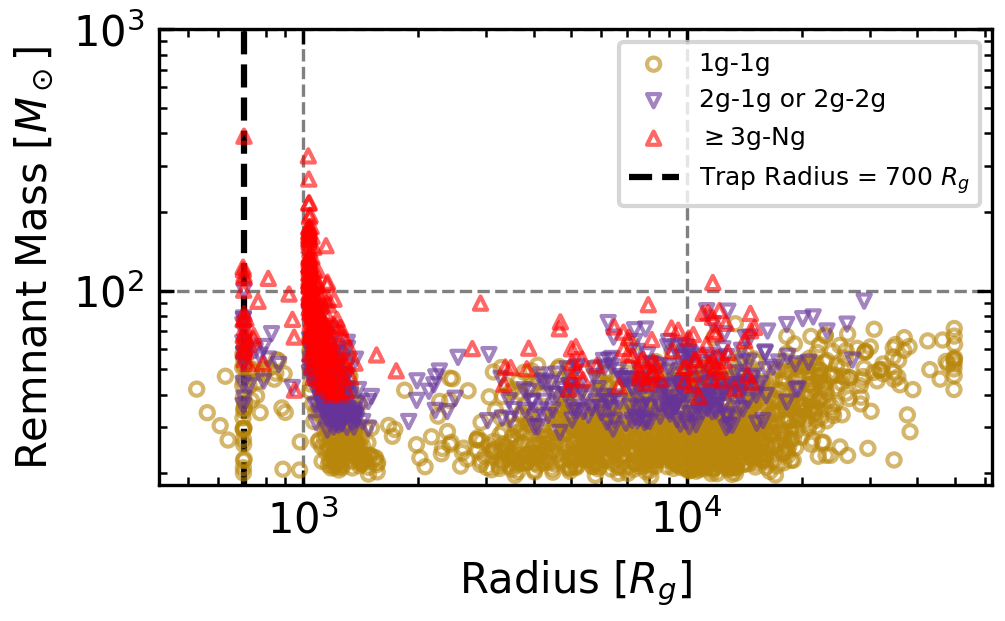
\includegraphics[width=0.5\textwidth]{ch_agnbbh_figs/p123_1Myr_ec9_merger_mass_v_radius.png}
      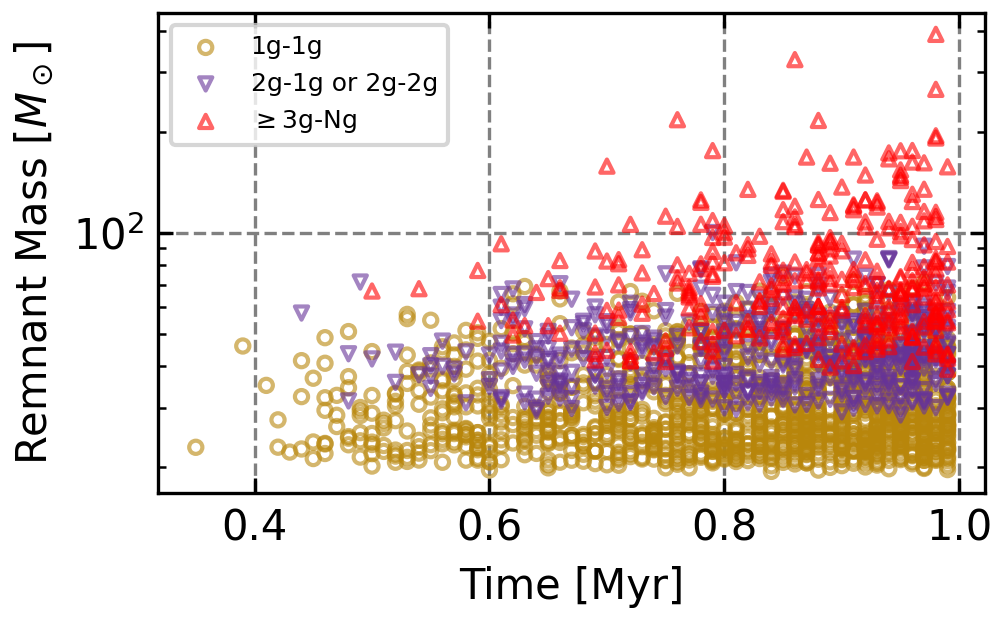
\includegraphics[width=0.5\textwidth]{ch_agnbbh_figs/p123_1Myr_ec9_time_of_merger.png}
	\caption[Disk lifetime of 1 Myr]{\textbf{Disk lifetime of 1 Myr.} As Fig.~\ref{fig:dyn-ecc} except disk runs for 1Myr. Input file and parameters are as in Fig.~\ref{fig:dyn-ecc} except \texttt{timestep\_num = 100}. Equivalent merger rate is ${\mathcal{R}} \sim 41.2 {\rm Gpc}^{-3} {\rm yr}^{-1}.$
   }
    \label{fig:sg_dyn_on_5Myr_time}
\end{figure*}


Fig.~\ref{fig:qX} illustrates the $q$--$\Xeff$ distribution for our default model, assuming the retrograde:prograde fraction of BBH mergers is $0(0.1)$ in the left(right) panel. Most mergers are 1g-1g and center around $\Xeff=0$. Higher generation mergers ($ng-mg$) ($n\geq 2,m \geq 1$) are mostly displaced to $|\Xeff| \sim [0.3,0.7]$ with more massive primaries typically having a spin that dominates the $\Xeff$ calculation. The width of the 1g-1g distribution depends on the choice of initial BH spin magnitude distribution and the extent of the 1g-1g distribution in $q$ is a function of the BH IMF ($M_{\rm BH,min/max}$). Thus, the $q$--$\Xeff$ distribution is an effective test of the BH IMF and spin distribution in galactic nuclei.
A full parameter space study can be found in \citep{Cook+25}.


\subsection{Testing AGN disk models}
\label{sec:disks}
We picked two AGN disk models to test, namely \citet{SirkoGoodman03} and \citet{ThompsonQuataertMurray05}.
Our default model is \citet{SirkoGoodman03} since this tends to give a better fit to the UV `big blue bump' in quasar spectral energy distributions and we expect that dense quasar disks are more efficient at coagulating embedded populations. In the case of \citet[][hereafter TQM]{ThompsonQuataertMurray05}, this disk model is less dense, less optically thick and at least nominally allowed to have a migration trap at $500\Rg$ \citep{Bellovary+16}, although this is likely due to an incorrect modelling of opacities \citep{DittmannMiller20}.

For reference, \Fig{fig:sg-disk} from the \citet{SirkoGoodman03} shows their disk radial profiles for an SMBH mass $\Mbh=10^8\,\Msun$ and Eddington ratio $l_\text{E}=L_0/L_\text{E}=0.5$ where the Eddington luminosity $L_\text{E} = \epsilon\dot{M}c^2$ for a non-self-gravitating disk with mass accretion rate $\dot{M}$ and $\epsilon=0.1$.
In comparison, \Fig{fig:tqm-disk} from \citet{ThompsonQuataertMurray05} shows their disk radial profiles for $\Mbh=10^9\,\Msun$, the mass accretion rate feeding the outer edge of the disk $\dot{M}_\text{out}=320\,\Msun\ \text{yr}^{-1}$ at $R_\text{out}=200$ pc, and a mach number $\text{Ma}=v/\cs=0.2$.

\begin{figure}
\centering
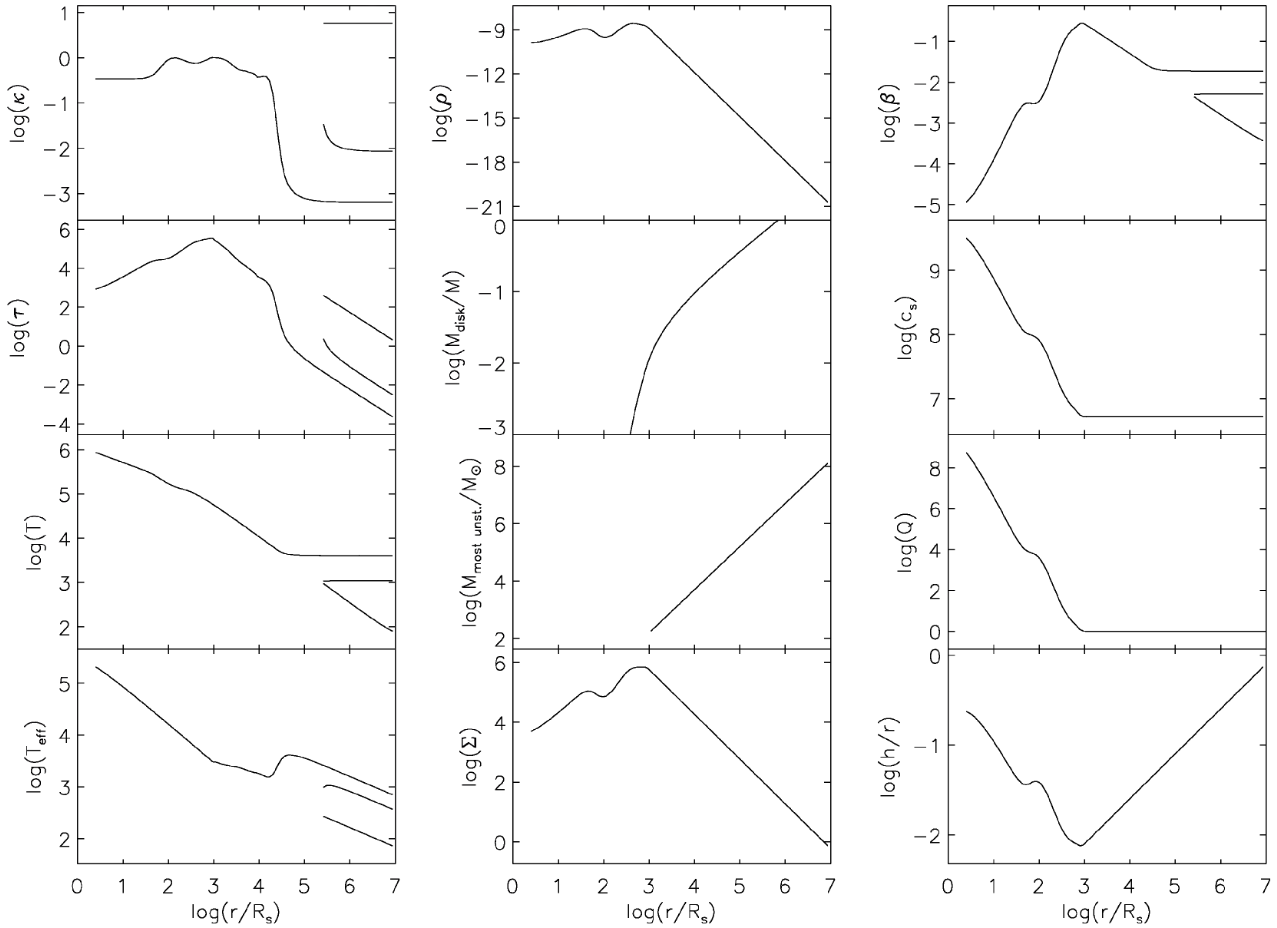
\includegraphics[width=1\textwidth]{ch_agnbbh_figs/sg_disk.png}
	\caption[Sirko and Goodman disk model]{\textbf{Sirko and Goodman disk model.} Radial AGN disk profiles for $\Mbh=10^8\,\Msun$ and $l_\text{E}=0.5$.
Reproduced from \citet{SirkoGoodman03}.}
\label{fig:sg-disk}
\end{figure}

\begin{figure}
\centering
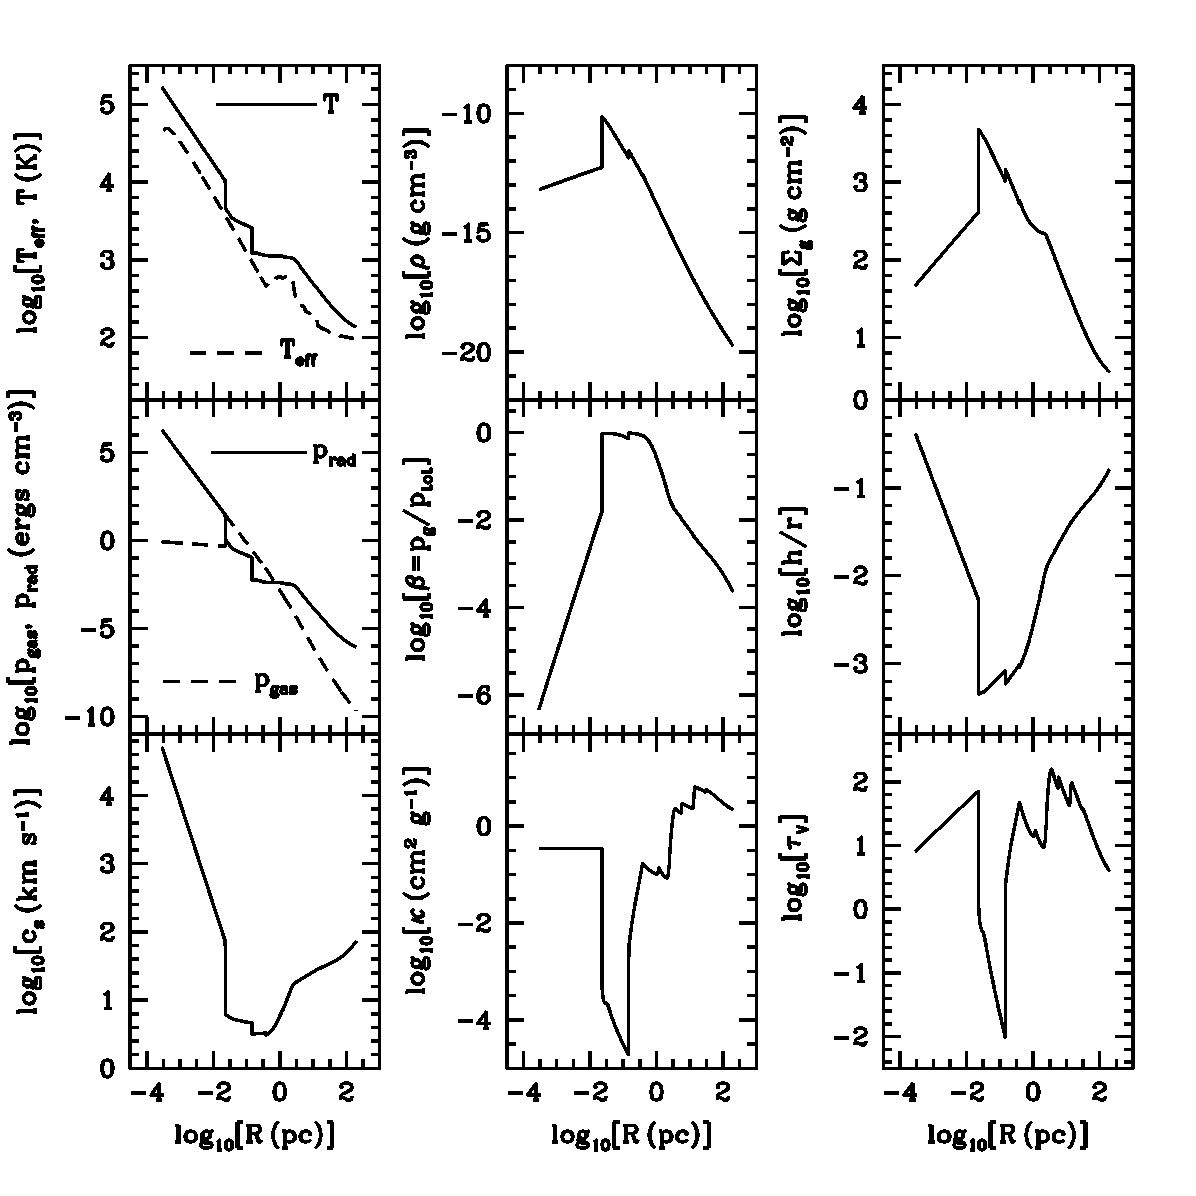
\includegraphics[width=1\textwidth]{ch_agnbbh_figs/tqm_disk.pdf}
	\caption[Thompson, Quataert \& Murray disk model]{\textbf{Thompson, Quataert \& Murray disk model.} Radial AGN disk profiles for $\Mbh=10^9\,\Msun$, $\dot{M}_\text{out}=320\,\Msun\,\text{yr}^{-1}$, $R_\text{out}=200$ pc, and $\text{Ma}=0.2$.
Reproduced from \citet{ThompsonQuataertMurray05}.}
\label{fig:tqm-disk}
\end{figure}


Fig.~\ref{fig:tqm_default} shows the distribution of BBH masses as a function of disk radius (left panel) and merger time (right panel) for our default \citet{ThompsonQuataertMurray05} model. Evidently, a less dense disk drives a significantly lower average merger rate ($\sim 0.1 \,{\rm Gpc}^{-3}{\rm yr}^{-1}$) than the \citet{SirkoGoodman03} model and the formation of new BBH becomes more difficult. The LVK AGN channel is likely filled with contributions from both high and low density disks.  Thus, in future work, we will introduce a prior spheroid binary fraction, which could be hardened towards merger, even in very low density AGN disks and which might dominate their contribution to the observed rate.

\subsection{Towards constraints on AGN lifetime}
\label{sec:time}
Fig.~\ref{fig:sg_dyn_on_5Myr_time} shows BBH merger masses as a function of location in disk and time for our default model run for 1Myr with $\rm{e}_{\rm max}=0.9$. The patterns observed in the shorter lived disk model Fig.~\ref{fig:dyn-ecc} persist (left panel) and mergers are delayed by $\sim 0.4{\rm Myr}$ by damping from a higher average initial eccentricity (right panel). The average equivalent merger rate is $\mathcal{R} \sim 41.2\,{\rm Gpc^{-3} yr^{-1}}$. As we limit the AGN fraction of LVK mergers, we will gain strong constraints on the average $\tau_{\rm AGN}$ and we will explore this in future work.


\subsection{Testing GW multi-wavelength models}
\label{sec:gw}
BBH that merge in AGN will be detectable across multiple GW frequencies ($\nu_{\rm GW}$) given by
\begin{equation}
    \nu_{\rm GW} = \frac{G^{1/2}M_{\rm BBH}^{1/2}}{\pi a_{\rm BBH}^{3/2}}
\end{equation}
where $G$ is the universal gravitational constant, $M_{\rm BBH}$ is the BBH total mass and $a_{\rm BBH}$ is the semi-major axis of the BBH around its own center of mass. The resulting gravitational wave strain is
\begin{equation}
    h = \sqrt{\frac{32}{5}} \frac{G^{2}}{c^{4}}\frac{M_{\rm BBH}\mu_{\rm BBH}}{D a_{\rm BBH}}
\end{equation}
with $c$ the speed of light, $\mu_{\rm BBH}=M_{1}M_{2}/M_{\rm BBH}$ is the BBH reduced mass, where $M_{1,2}$ are the masses of the individual BBH components and $D$ is the distance to the BBH. Importantly, in AGN, binary black holes (BBH) can form between two stellar mass BH, but also between individual stellar mass BH and the central SMBH. The latter (SMBH-BH binaries) will be detectable at low GW frequencies as extreme mass ratio inspirals (EMRIs) with LISA \citep{LISA23}.

As BBH evolve (due to gas hardening/softening, binary softening/hardening or GW emission) they change their GW frequency. A useful parameter, the characteristic strain, averaged over all polarizations is
given by $h_{\rm char} = (N/8)h$ where $N = \sqrt{2\nu_{\rm GW}^{2}/\dot{\nu}_{\rm GW}}$ and $\dot{\nu}_{\rm GW}=\mathcal{M}_{\rm ch}^{5/3}\nu_{\rm GW}^{11/3}$ where the binary chirp mass $\mathcal{M}_{\rm ch}=(M_{1}M_{2})^{3/5}/M_{\rm BBH}^{1/5}$ if $\nu_{\rm GW}>10^{-6}\,{\rm Hz}$. 

Fig.~\ref{fig:gw_strain} shows the characteristic strain  ($h_{\rm char}$) as a function of gravitational wave frequency ($\nu_{\rm GW}$) assuming all AGN are located at $z=0.1$ by default. For detailed simulations and predictions of redshift dependency of the outputs produced by \code{McFACTS} as a function of $M_{\rm SMBH}$ and NSC properties see \citet{Delfavero+25-mcfactsIII}. Curves in blue (orange) correspond to the LISA (LIGO Hanford O3) sensitivity curves respectively. Note that the LIGO curve is appropriate for $h_{0}$ rather than $h_{\rm char}$. Points in blue correspond to snapshots at the end of each default timestep of EMRIs from 100 iterations of the default model (see Ford et al. 2026 in prep.). Points in gold, purple, red correspond to snapshots of 1g,2g and $\geq 3$g BBH at the end of each timestep of individual BBH with $\nu_{\rm GW}>10^{-7}\,{\rm Hz}$. 

On average $2-3$ points are associated with each BBH, since our default gas hardening prescription \citep{Baruteau11} drives rapid mergers of hard binaries. Once a BBH shrinks to a point where it will merge within the next timestep ($\mathcal{O}(10^{-3}{\rm Hz})$ for default), $\dot{\nu}_{\rm GW}$ in $N$ above is switched from gas-hardening to GW hardening \citep{Peters64}, leading to the break in $h_{\rm char}$ around $\sim 10^{-3}{\rm Hz}$  The first BBH point is arrival in the LISA frequency band on a single timestep, a second BBH point is the evolved BBH in the next timestep, which could correspond to a merger in the LIGO band, or a dynamically hardened/softened BBH (see Postiglione et al. 2026 for a detailed study, and for an illustration of the range of possible BBH merger tracks). BBH that enter the LISA band, but are then ionized, are typically represented by a single point on this plot.  The band of gold, red and purple points correspond to snapshots of BBH mostly gas-hardening towards merger with typical value of $h_{\rm char} \approx \mathcal{O}(10^{-22})$. 
Since binary hardening or softening in the code is either gas-driven or dynamics driven, we have not yet combined gas and dynamics hardening in a given timestep. More sophisticated treatment of both gas and dynamical hardening will be treated in future work ({Postiglione et al. 2026 in prep.}), particularly with a view to testing LISA detectability of gas and dynamically hardened AGN channel BBH. 

\begin{figure}   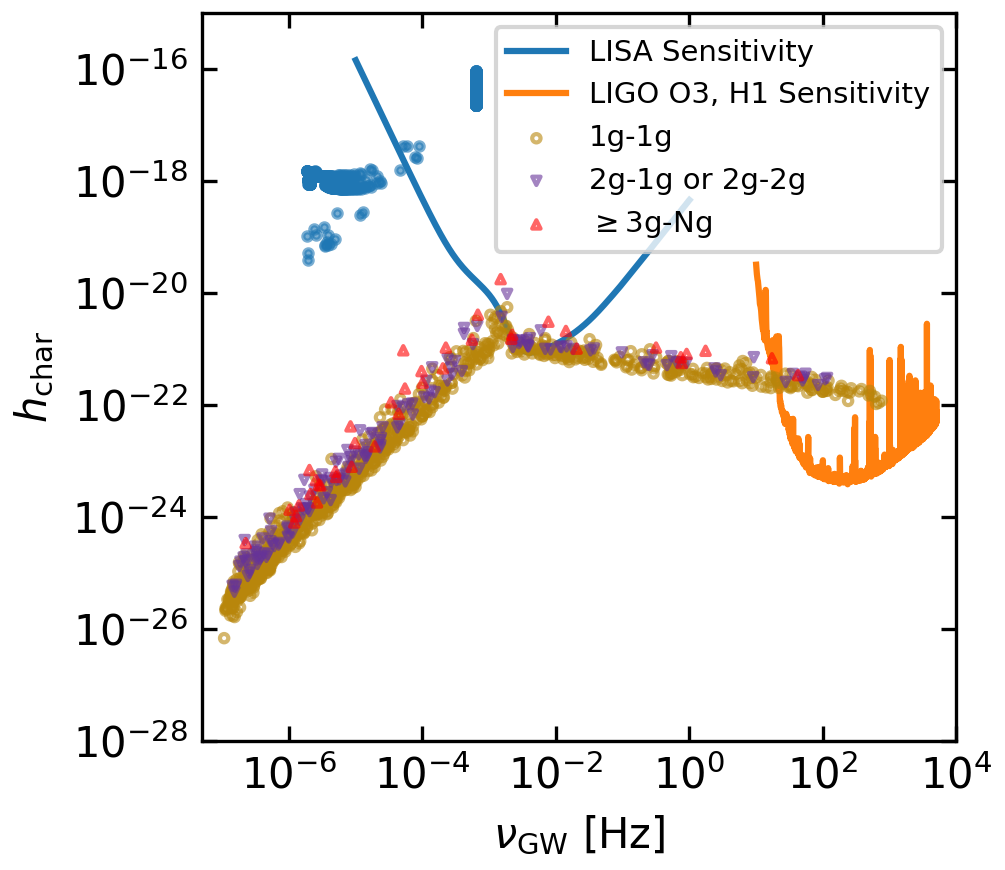
\includegraphics[width=1\textwidth]{ch_agnbbh_figs/gw_strain.png}
	\caption[Characteristic strain vs. frequency]{\textbf{Characteristic strain ($h_{\rm char}$) as a function of GW frequency ($\nu_{\rm GW}$)} after a 0.5Myr episode with default AGN model assumed to lie at $z=0.1$. Note that the LVK sensitivity curve is appropriate for $h_{0}$ rather than $h_{\rm char}$ (see Postiglione et al. 2026 in prep. for a more accurate treatment). Input file and parameters are as in Fig.~\ref{fig:dyn-ecc}.
    }
    \label{fig:gw_strain}
\end{figure}

In \code{McFACTS}, EMRIs form when a BH arrives within $a<50\,\Rg(M_{\rm SMBH}/10^{8}\,M_{\odot})^{-1}$ of the SMBH. The rate at which BH appear at such small disk radii is strongly effected by two factors: first, the number of retrograde embedded BH initially in the disk and second, the rate of disk capture and the range of allowed capture radii. 

When an AGN disk arrives in a relaxed galactic nucleus population, around half of the initial population of orbiters embedded in the disk will have orbits that are retrograde with respect to the disk gas. Depending on their semi-major axis and the disk surface density profile, the gas can excite the orbital eccentricity of embedded retrograde BH to large values, potentially generating a population of BH at small disk radii \citep{Secunda+21}. However, perturbations of orbital inclination of embedded retrograde orbiters, due to e.g. turbulence, or interactions with spheroid orbiters, will tend to drive the retrograde orbiters out of the disk and tend to rapidly flip them to prograde \citep{WangZhuLin24}. This initially retrograde population in a turning-on AGN will tend to drive a high EMRI rate (these correspond to the vertical line of blue points at $\nu_{\rm GW} \sim 10^{-3}{\rm Hz}$ in Fig.~\ref{fig:gw_strain} and see {Ford et al. 2026 in prep.}). After multiple short-lived AGN episodes in the same nucleus, the retrograde fraction in the disk should become very small, so the LISA EMRI rate should be highest in new AGN episodes in relatively relaxed galactic nuclei (Ford et al. 2026 in prep.).

Under default models, the disk captures BH uniformly at radii $a<2\times 10^{3}\,\Rg$ every 0.1Myr, so there is a $2.5\%$ chance of an EMRI every disk capture under default assumptions. EMRIs are considered to only evolve under the evolution of GW emission (gas effects are ignored for now). So in Fig.~\ref{fig:gw_strain} the characteristic strain per frequency (equivalently the amount of time at a monochromatic 
 GW frequency) decreases as the EMRI shrinks (as $\nu_{\rm GW}$ increases). The exception occurs during the chirp at merger where $h$ increases dramatically. Some EMRIs form late in a run or at large enough distance ($\sim 50\,\Rg$) and do not chirp within the 0.5Myr lifetime. These correspond to the population at lower characteristic strain ($h_{\rm char}/\nu_{\rm GW} \sim 10^{-19}$ in Fig.~\ref{fig:gw_strain}).
 
\subsection{Conclusions}
\label{sec:mcfacts-conclusions}

We demonstrate the new, public, open source, fast and reproducible code $\code{McFACTS}$ , the Monte Carlo For AGN channel Testing and Simulation. \code{McFACTS} allows rapid testing of BBH merger properties across AGN and NSC parameter space. Users can choose their own AGN disk model or NSC model and quickly get population statistics and distributions of parameters. The code as released (\code{v.0.3.0}) makes multiple simplifying assumptions but is intended to be a living, developing code (see \sect{sec:chapter-future} for planned near-future additions).

We illustrate the code and demonstrate its performance by varying AGN and NSC parameter inputs and show that a high average rate ($\mathcal{R}$) of BBH mergers in the AGN channel is generally associated with relatively dynamically cool populations of BBH in short-lived AGN.
This may imply a strong contribution to the LVK AGN channel from AGN fuelled by pulses of low angular momentum gas in the same plane from a fuel reservoir.
For a study of mergers in AGN as a function of NSC model, Galaxy mass and redshift, see \citet{Delfavero+25-mcfactsIII}.
The next chapter will present a detailed studies of the AGN channel in $q$--$\Xeff$ parameter space published in \citet{Cook+25}.



\clearpage
\resetcounters
\addtocontents{toc}{\protect}
\section{\texorpdfstring{\MakeUppercase{active galactic nuclear accretion disk influence on the mass ratio and effective spin plane}}{active galactic nuclear accretion disk influence on the mass ratio and effective spin plane}}
\label{sec:qXeff}

\counterwithin{figure}{section}
\counterwithin{table}{section}

\par The model and results described in this chapter were produced using the \mcfacts code that was initially published in a series of papers \mcfacts \code{I}
\citep{McKernan+25-mcfactsI}, \mcfacts \code{II} \citep{Cook+25}, and \mcfacts \code{III} \citep{Delfavero+25-mcfactsIII} in the \textit{Astrophysical Journal}.
The bulk of this chapter is directly informed by the content of \citet{Cook+25}, my primary scientific contribution, with my contributions to the other papers mixed in.
I will also briefly summarize the first paper in the series, \citet{McKernan+25-mcfactsI}, for algorithmic reasons and in the capacity that pertains to my work.
Please refer to \citet{McKernan+25-mcfactsI} for specific model details and \citet{Delfavero+25-mcfactsIII} for results related to a cosmologically informed galaxy population.

\subsection{Motivation}

Here we present a study using the \mcfacts code \citep{McKernan+25-mcfactsI, Cook+25, Delfavero+25-mcfactsIII} to test the predictions of the AGN channel for the $q$--$\Xeff$ distribution across a wide range of parameter space in both AGN disk and NSC models, with a view to tightly constraining requirements on the AGN channel.
The assumptions we vary include the BH initial mass function (IMF), disk model, disk size, disk lifetime, NSC model, and the prograde-to-retrograde fraction of newly formed black hole binaries.
\mcfacts features substantial improvements to the Monte Carlo code used in \citet{McKernan+20a} to explore $\Xeff$ of mergers in AGN and \citet{McKernan+22:q-Xeff} who explored the $q$--$\Xeff$ anti-correlation.
The greater flexibility for exploring parameter space includes many improved models for disk-NSC interactions such as dynamical encounters, orbital migration, and binary evolution.
Broadly we find that dense, moderately short-lived AGN disks are preferred for producing an anti-correlation between the mass ratio $q$ and effective spin $\Xeff$ like has been identified from existing GW observations.
Additionally, when populating the disk with BHs from the IMF, the likelihood of drawing a given BH with mass $M$, we find a preference for $p(M) \propto M^{-2}$ over a more top-heavy IMF ($M^{-1}$).
The preferred fraction of prograde-to-retrograde is $>90\%$, to produce results consistent with observations.



\subsection{Background}
\label{sec:background-qxeff}
GW observations provide information about each component mass and spin for a given BBH merger.
In this work, we will focus on two specific BBH parameters: the binary mass ratio $q=M_2/M_1\ (M_1>M_2)$, where $M_{1}$ and $M_{2}$ are the primary and secondary BH masses; and effective spin of the BBH as given by 
\begin{equation}
\label{eqn:Xeff}
	\Xeff = \frac{M_{1}\vec{\chi}_{1} + M_{2} \vec{\chi}_{2}}{M_{1}+M_{2}}\cdot \hat{\vec{L}}_\text{bin}
\end{equation}
where $\vec{\chi}_{1,2}$ are the dimensionless spin parameters associated with $M_{1},M_{2}$ respectively and $\hat{\vec{L}}_\text{bin}$ is the direction of the orbital angular momentum vector of the BBH.

\begin{figure}
	\centering
	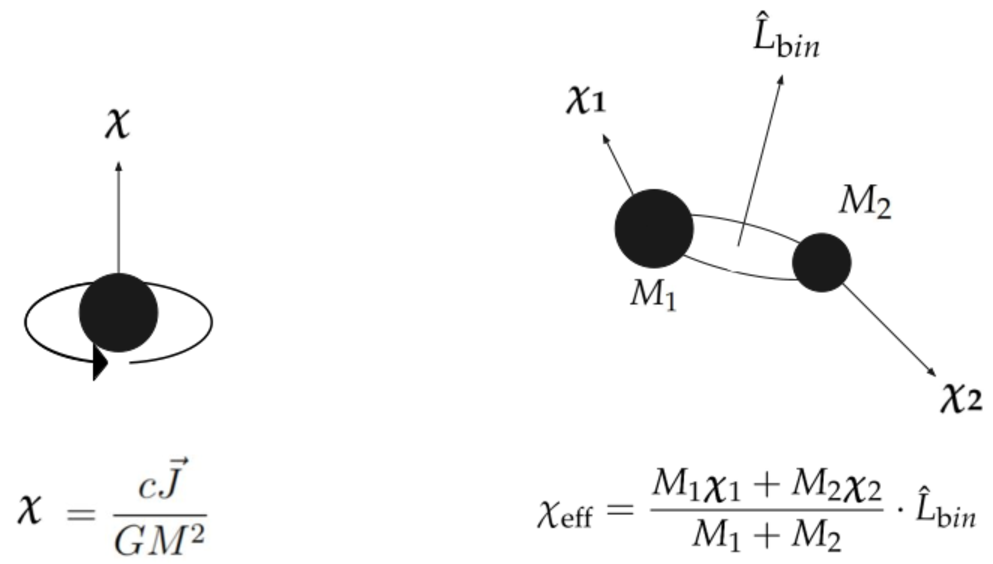
\includegraphics[width=1\textwidth]{ch_qxeff_figs/xeff-diagram-eqns.pdf}
	\caption[Effective Spin Diagram]{Diagram of the components in Eq.~\ref{eqn:Xeff} needed to calculate the effective spin $\Xeff$ measured for a merger event.}
	\label{fig:xeff-cartoon}
\end{figure}


\begin{figure}
	\centering
	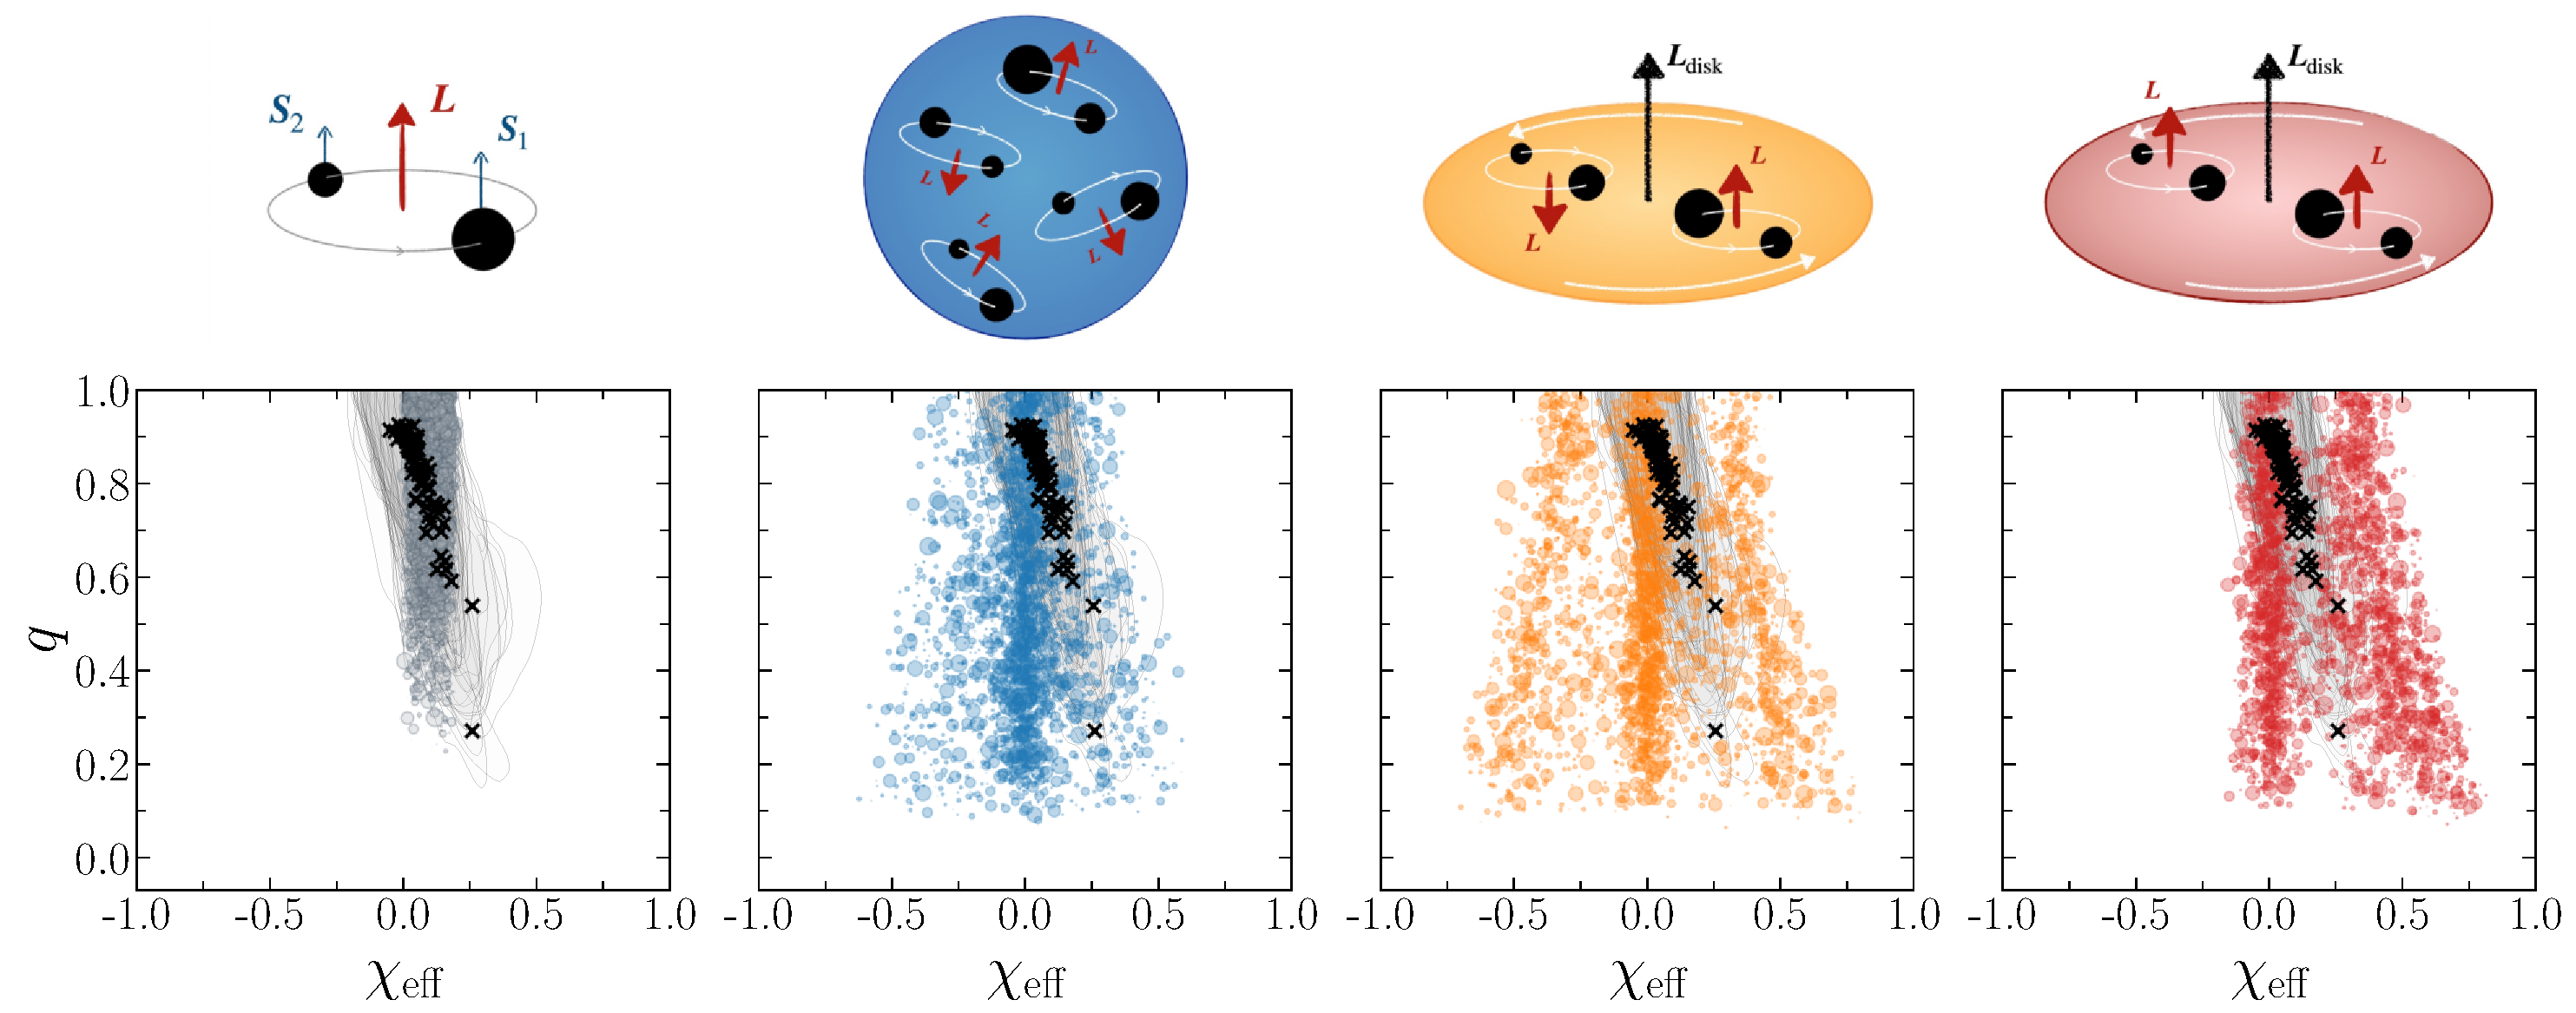
\includegraphics[width=1\textwidth]{ch_qxeff_figs/santini+23_qxeff_channels.pdf}
	\caption[The $q$--$\Xeff$ plane for different formation channels]{The $q$--$\Xeff$ distributions for BBH mergers originating in various binary formation channels.
	\emph{Left:} Isolated field binary stars.
	\emph{Left of center:} Globular clusters.
	\emph{Right of center:} AGN disks with retrograde and prograde binary angular momenta.
	\emph{Right:} AGN disks with only prograde binary angular momenta.
	Figure taken from \citet{Santini+23}.
	}
	\label{fig:qxeff-channels}
\end{figure}

There are several formation channels for forming BBH.
\citet{Santini+23} explored how the $q$--$\Xeff$ plane would appear like for three possible formation scenarios shown in \Fig{fig:qxeff-channels}, which is reproduced from their paper.
The left panel shows this for binary stellar companions whose orbits are close enough to experience periods of common-envelope evolution, that cause their orbits to shrink enough for GW radiation to shrink their orbits further.
In this scenario it is most likely that both stars formed from the same molecular cloud and have parallel rotational angular momentum which restricts $\Xeff$ to be positive.
Another common pathway for BBH formation is through dynamical interactions in globular clusters and NSCs shown in the left-of-center panel.
In these environments stars and black holes frequently encounter each other, exchanging partners, and shrinking their orbits, again, until GW radiation takes over.
Binaries formed here will have randomly oriented spins, and $\Xeff$ can be either negative or positive but will be evenly distributed about $\Xeff=0$.
As discussed in the previous chapter, the presence of an accretion disk will align orbits of NSC objects to be fully embedded within its confines over time \citep{Fabj+20,Nasim+22}.
Thus, when binaries form due to encounters along similar trajectories, $\hat{\vec{L}}_\text{bin}$ will preferentially align with the disk orbital angular momentum, causing $\Xeff$ to be more restricted than when no disk is present despite the fact that $\vec{\chi}_i$ for any newly captured BH will be randomly oriented, as shown in the right panels.
Since merger remnants primarily inherit their spins from $\hat{\vec{L}}_\text{bin}$, $\Xeff$ becomes progressively more aligned or anti-aligned with the disk depending on whether both prograde $\hat{\vec{L}}_\text{bin} \cdot \hat{\vec{L}}_\text{disk} = +1$ and retrograde $\hat{\vec{L}}_\text{bin} \cdot \hat{\vec{L}}_\text{disk} = -1$ or only prograde binaries form.
Merger remnants in dynamical channels are more likely to merge again in what is called a hierarchical merger scenario, each time increasing their mass and spin, which is reflected in the wider distribution in $\Xeff$ at low $q$ since more massive BHs are more likely to capture less massive companions.


Throughout this chapter we will refer to a BH that formed through stellar evolution processes as a first generation, or a 1g, BH.
Each merger event increases the generation of the highest generation component by one such that a 2g$-$4g merger event produces a 5g remnant.
We categorize merger events into three groups based on the generations of the BH involved: (1) 1g mergers between first generation BH (1g-1g), (2) 2g mergers involving second generation BH (2g-1g and 2g-2g), and (3) $\geq$3g mergers involving a third generation BH or higher (3g-Ng).

For intuition in what follows, the range of $q$ among first generation (1g; BH produced via stellar evolution) mergers will depend on the range of the IMF (e.g., $10\leq M/\Msun \leq 40$) as well as the power-law of the mass distribution ($\propto M^{-\gamma}$).
A steeper mass function with $\gamma = 2$ biases the distribution towards lower mass BH and therefore implies a bias towards $q \sim 1$ as binaries are more likely to form between similar mass BH.
A shallower mass function with $\gamma = 1$ permits a higher relative fraction of high mass BH and by extension pairings between a broader range of masses, driving $q$ lower.

Drawing spins ($\vec{\chi}_{1,2}$) from a uniform distribution between those that are aligned and anti-aligned with $\hat{\vec{L}}_\text{bin}$ means that the resulting $\Xeff$ distribution should be centered on $\Xeff \sim 0$, with the width of that distribution a function of the initial spin magnitudes $|\vec{\chi}_{1,2}|$; see, e.g., \cite{Callister21} for details.
However, a bias towards prograde BBH formation in the AGN channel would favor positive $\Xeff$ values in general.
Such a bias might be due to orbital inclination flipping \citep{DittmannDempseyLi24} of an inclined BBH, preferential ionization of retrograde BBHs as they spend more time at wider separation \citep[on average,][]{Wang+21,Calcino+23}, or some other mechanism.
Additionally, once BBH merge, most of their orbital angular momentum as they coalesce will go into natal spin of the newly merged BH, typically $\chi \sim 0.7$ \citep{TichyMarronetti08}.
Thus, hierarchical mergers containing higher generation (2g or higher) BH that have inherited these large positive spins will therefore strongly favor positive $\Xeff$.

\subsection{Major contributions to \mcfacts}

\mcfacts is developed by a large team, and I was present from the beginning and involved with many design decisions and development.
While I made many contributions, I will highlight two of them here: the Monte Carlo method and a broken power-law distribution for assigning BH locations in the NSC.

The core purpose of \mcfacts is to generate statistical populations of BH mergers produced through an algorithm replicating the physical processes present in the AGN formation channel.
This requires the ability to repeatedly simulate those processes under slightly varying conditions to understand individual and cumulative effects of those variations.
Monte Carlo methods are used for this purpose because they allow repeated random sampling of quantities from a range of possible values that are assigned a probability of being drawn from the population, i.e. a probability distribution.
After we established the algorithm for evolving BHs in an AGN disk for a single galaxy, I implemented a pseudo-random number generator (PRNG) that allows us to set an initial random state using a unique seed.
The generator is not truly random because this seed introduces a deterministic sequence that means the randomness is not unpredictable.
This is a fundamental issue in cybersecurity but our code does not encrypt data or contain sensitive information.
The pseudo-randomness is necessary for the work since the seed gives us the ability to start the generator at the same state for each run. 
Then, each time we need to draw a number to assign a BH its mass or to select the orbital parameters after a dynamical encounter we invoke the same random number generator which advances its state with each draw.
This functionality is a core aspect of scientific reproducibility that allows us to control experimental setups with better understanding of the outcomes.

One of the probability distributions we use assigns the initial location of a BH in the AGN disk.
I implemented a mechanism to draw these values by selecting one of the following probability distributions: 1) uniform distribution 2) broken power-law distribution.
A uniform distribution assumes BHs have equal probability of existing at every radius in the disk, but it is only included as an optional setting for cases a user may find it useful and is not appropriate for determining BH distributions across large regions of the NSC.
Our NSC model is defined with a broken power-law number density profile that goes as $n\propto R^{-7/4}$ out to a critical radius at $R\sim 0.25$ pc where the index changes to $n\propto R^{-2.5}$ out to $5$ pc and contains $10^4$ BHs within the central $\text{pc}^3$ \citep{Generozov+18}.
If implemented directly, this distribution inaccurately allocates a greater probability density to the inner disk that, if used, would artificially over-crowd it with BHs.
To correct for this, we normalize the radial grid by the critical radius as
\begin{equation}
	p(R) = \left( \frac{R}{\Rcrit} \right)^\eta
\end{equation}
using the correct power-law index $\eta$ as is appropriate relative to $\Rcrit$.
Then, we scale the probability in each bin of the radial grid by its corresponding shell volume
\begin{equation}
	p(R) = \frac{p(R)}{\pi R^2 \Delta R}
\end{equation}
where $\Delta R$ is the width of the radial bin.
The final probability density distribution is shown in \Fig{fig:nsc-loc-sampling} by the purple shaded region alongside those for the uniform distribution (red) and unscaled broken power-law distribution (teal).
Also plotted are histograms of the resulting draws for 100 galaxies where the disk radius is $\Rout=10^6\,\Rs$, replicating the initial samples for a typical run in \mcfacts.
The radius is extended here beyond $\Rout$ used in this work to demonstrate the shape of the broken power-law distribution and the BH populations in comparison with the uniform distribution.
Importantly, a uniform distribution under-populates the region near $\Rcrit$ and over-populates in the outer disk.
The population generated with the unscaled power-law probability distribution is so concentrated in the first bin that only $\sim1200$ BHs get initialized beyond it.
The $y$-axis is trimmed to ignore most of these to highlight the complexity in the outer disk.




\subsection{Methods}
\label{sec:methods-qxeff}

Here we introduce the assumptions, models, and parameters that we vary in the \mcfacts code relevant for testing the $q$--$\Xeff$ distribution.
We run each of the following setups 100 times to build a statistically significant sample.
In each run, our code evaluates the following physical processes:

We begin by generating a disk model using the \code{pAGN} code \citep{Gangardt+24-pAGN} using the default parameters for a SMBH with mass $\Mbh=10^8\,\Msun$.
The default extent is $5 \leq R/\Rg \leq 5\times10^5$ with the alpha viscosity parameter $\alpha=0.01$, and a lifetime depending on the disk model (see below).

The next step is to populate the disk with BHs using a broken power-law distribution dependent on the power-law indices of the number density profiles as defined by \citet{Generozov+18}.

We draw masses for each BH from a Pareto distribution IMF with index $M^{-2}$ over the range $10<M/\Msun<40$.
To replicate the slight over density observed at $35\,\Msun$ \citep{Abbott+23-massbump}, we redraw for any BHs that would be assigned a mass above this range from a Gaussian with width $2.3\,\Msun$ centered at $35\,\Msun$.
The initial BH spins are drawn from a Gaussian centered on dimensionless spin parameter $\chi=0$ and width $0.2$, and the radial locations are drawn from a volume-normalized probability distribution according to the NSC power-law structure.
Finally, the orbital eccentricity is drawn from a uniform distribution in $e^2$ over the range $0<e<\emax$ and randomly assigned as a prograde or retrograde orbit according to a uniform distribution with the retrograde fraction set by $0<\fret<1$.
BHs on retrograde orbits around the SMBH are more challenging to consider, and at the time of this work they are populated in the initial conditions but they are not allowed to interact with the prograde population and the equations governing their orbital evolution are not fully implemented.

\begin{figure}
\centering
	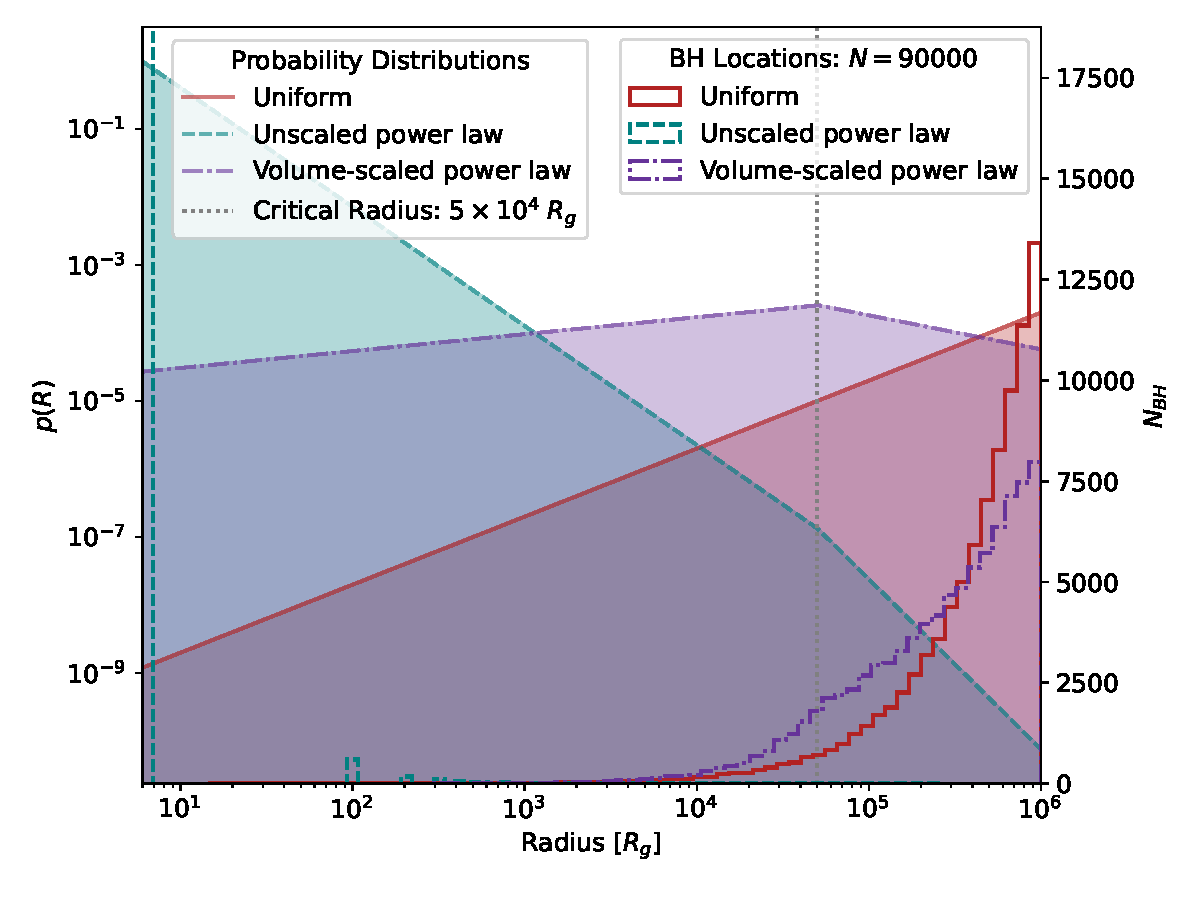
\includegraphics[width=1\textwidth]{ch_qxeff_figs/probability_and_histogram_900bh_100gal_1e+06Rg.pdf}
	\caption[Sampling black holes from a nuclear star cluster]{Probability densities and resulting population of BH drawn from a NSC for a uniform distribution (red, solid line), a broken power-law (teal, dashed line), and the same broken power-law with proper volume scaling (purple, dash-dotted line).}
\label{fig:nsc-loc-sampling}
\end{figure}

AGN disk gas can circularize eccentric orbits \citep{McKernan+12} over time or pump eccentricity if the density increases with radius \citep{Secunda+21}. 
Once orbits become circular, radial migration can occur both inward and outward depending on the disk conditions, at which point BHs may encounter each other to form BBHs, which we set to occur when their separations are within one Hill's radius of the more massive BH.
While most binaries will likely form from the circularized population, they can still interact with BHs on elliptical or inclined orbits.
Gas effects and dynamical encounters with a third BH can cause the binary to lose energy (harden) or gain energy (soften).
Once BBHs are sufficiently hardened, further energy loss due to GW radiation becomes poss until they merge \citep{Peters64}.
Merger recoils put BH remnants on eccentric orbits where the process continues or removes them from the disk.
Finally, gas torque acting on disk-crossing BH orbits replenishes the embedded BH population from the NSC \citep{Fabj+20,Nasim+22}.

\subsubsection{Disk Models}
As we cannot yet observationally resolve them, the physical conditions of AGN disks are poorly constrained.
Instead we rely on model fits to spectroscopic and multi-wavelength variability data.
We use two common one-dimensional radial models, namely, SG \citep{SirkoGoodman03} and TQM \citep{ThompsonQuataertMurray05}.
The inner regions of the SG disk are likely to be more accurate than the outer regions where assumptions are made to prevent the disk from collapsing due to gravitational instability.
In contrast, the star formation models supporting the outer regions of the TQM model are more accurately implemented, but the model's opacity for inner disk annuli are likely too low.
For both models we truncate the disk at some outer value $R_{\rm out}$, assume the disk lives in a steady state for time $\tauAGN$, and use the \code{pAGN} code to construct our disk models \citep{Gangardt+24-pAGN}.

Analogous to protoplanetary disks, migration traps and anti-traps may form between regions of outward and inward migration \citep{Lyra+10}.
We calculate migration torques for circular BH orbiters (singles and binaries) and change their semi-major axes depending on their location relative to user-defined traps according to \citet{Paardekooper+10} as implemented in \citet{GrishinGilbaumStone24}.
We consider the additional influence of radiative feedback from accretion \citep{HanklaJiangArmitage20} that reduces the strength of inward migration torques and can even turn them outward.
Following \citet{Bellovary+16}, we set migration traps at 700 $\Rg$ in SG disks and 500 $\Rg$ in TQM disks.
In practice, mergers also aggregate near $R\sim10^3\,\Rg$ (for $\Mbh = 10^8\,\Msun$) when using migration prescriptions described by \citet{GrishinGilbaumStone24} as BH enter the region of lower migration speeds as they approach the trap.

The choice of migration torque model may be important for disk structures around SMBH of different mass, and \mcfacts provides the user with two options: a two-dimensional model from \citet{Paardekooper+10} and a three-dimensional (3D) model from \citet{JimenezMassset17}.
In general, the Jim\'enez-Masset 3D torques are weaker across the bulk disk by up to $\sim$30\%.
This tends to drop the overall merger rate in disks (including at the trap if present).
Likewise migration traps move radially outward in units of $\Rg$ as the SMBH mass drops well below $\Mbh=10^8\,\Msun$, but in \citet{McKernan+25-mcfactsI} we compared these models and found little change for $\Mbh = 10^8\,\Msun$ \citep[see Fig. 6 \& 7 of][]{McKernan+25-mcfactsI}, which is also the SMBH mass we find that produces the most mergers \citep{Delfavero+25-mcfactsIII}.
Thus, we choose the simpler \citet{Paardekooper+10} torque model here and confine our study to disks around SMBH with mass $\Mbh = 10^8\,\Msun$.

\subsubsection{Initial Black Hole Properties}
We draw the initial BH masses from a Pareto distribution with $P(M) \propto M^{-\gamma}$ for $10\leq M/\Msun \leq40$, with an additional Gaussian component centered on $35M_{\odot}$ \citep[see][]{McKernan+25-mcfactsI}.
We use $\gamma=2$ as the default throughout this paper and vary it to $\gamma=1$.
We draw the initial BH spin directions $\hat{\chi}$ from a uniform distribution over the interval $[0,\pi]$ and the spin magnitudes from a Gaussian distribution centered at $\mu_\chi=0$ with standard deviation $\sigma_{\chi} = 0.1$ as the default and test variations to $\sigma_{\chi}=0.02$ and $0.2$.

\subsubsection{Disk Lifetimes}
AGN lifetimes ($\tauAGN$) are thought to lie in the range $\sim 0.1$ Myr \citep{Schawinski+15,Khrykin+19} to 10s of Myr \citep{Hopkins+05,Khrykin+21}.
The lifetime is important for regulating how long each disk process operates on the nuclear system.
We choose a default lifetime for SG disk models of $\tauAGN=0.5$ Myr and study variations of $\tauAGN = 0.25$ and 0.75 Myr.
Since the TQM disk is generally less dense which reduces the effectiveness of gas interaction processes, we increase the default lifetime to $\tauAGN = 3$ Myr with variations of $\tauAGN = 2.5$ and 5 Myr.

\subsubsection{Disk Size}
The disk outer radius $R_{\rm out}$ determines what portion of the NSC will interact with the AGN disk; thus it dictates how many BH will be embedded in the disk at the start of an AGN episode and how many NSC objects can be captured over the AGN disk lifetime.
Since opacity drives most of the processes affecting embedded BH, we use it to set $R_{\rm out}$.
The opacity of an SG disk roughly increases in the inner disk before dropping off significantly in the outskirts.
We set $R_{\rm out}$ to the radius at which the opacity decreases back to the value at the innermost disk radius, leading to a default disk size of $5\times10^4\,\Rg$, where $\Rg = G\Mbh/c^2$ is the gravitational radius with $\Mbh=10^{8}\Msun$ -- see Sec.~\ref{sec:smbh-mass}).
We adopt this value for the TQM disk since it also reaches a similar value as found at the innermost edge at $5\times10^4\,\Rg$, though the opacity behaves inversely with radius as compared to the SG model.
We expect larger disk sizes that intersect with a larger portion of the NSC to produce more mergers, although this depends on the NSC radial density profile.
Additionally, the initial pool of BH in a larger disk has greater distances through which to migrate and encounter possible companions that are unavailable in a smaller disk, possibly increasing the overall number of mergers.
As such, since larger objects migrate faster, they encounter more objects, so we might expect larger disk sizes to drive lower $q$ encounters.

\subsubsection{Orbital Eccentricity}
Gas drag induced by dynamical friction caused by Lindblad resonance torques \citep[referred to as Type I migration][]{GoldreichTremaine79,Ward97} can damp or pump orbital eccentricity $e$ of an embedded BH depending on the local conditions of the disk \citep{McKernan+12, Secunda+21, McKernanFord24, SzolgyenMacLeodLoeb22}.
Radiation from accreting objects can cause an additional eccentricity pumping term \citep{Cornejo+23}.
We compute the damping timescale according to \citet{TanakaWard04} via \citet{McKernanFord24} and apply \citet{PapaloizouLarwood00} exponential decay when $e<2H$ -- where $H$ is the pressure scale height -- and the characteristic decay timescale when $e>2H$ \citep{BitschKley10, Horn+12}.
Once the orbital eccentricity is sufficiently small, BH migration and BBH formation become efficient.
A relaxed (thermal) NSC has median eccentricity of $e=0.7$, but this requires a long duty cycle between AGN phases.
SMBH spins observed in the local Universe are predominantly high spin with $\chi>0.9$ for half of SMBH \citep{Reynolds19}, indicating they preferentially accrete along a consistent plane rather than randomly \citep{Volonteri+05}.
If AGN consist of short-timescale accretion episodes \citep{Schawinski+15,Shen21}, delivered from a fuel source in the same plane (possibly the dusty torus), this could drive consistent SMBH spin up over many AGN episodes.
In this case, the NSC populations would have little time to relax between episodes, keeping eccentricities relatively damped (low).

We draw initial orbital eccentricities $e_0$ from a uniform distribution between 0 and $e_{0,max}$ representing the maximum eccentricity achieved during the prior quiescent state.
Thus, a smaller value of $e_{0,max}$ implies a shorter relaxation time between accretion episodes according to the previously mentioned scenario.
We choose fiducial values for the maximum in SG disks to be $e_{0,max}=0.5$ and in TQM disk to be $e_{0,max}=0.05$.
The latter compensates for the lower density in TQM and correspondingly longer circularization timescales.
This choice assumes the NSC has insufficient time to fully relax between AGN disk episodes and that each such episode occurs in the same plane.
We also explore setting $e_0=0$ in the low density TQM model to bypass the long eccentricity damping time.

\subsubsection{Binary Formation}
We form BBH from the circularized BH population when the separation between adjacent orbits reaches one Hill radius ($\Rhill$) at the beginning of the time step, i.e. $\Delta a = |a_1-a_2| \leq 1\Rhill$, where $a$ is the semi-major axis, $\Rhill = a_1 \left( M_1/3\Mbh \right)^{1/3}$, $M_1$ is the more massive candidate, and $\Mbh$ is the mass of the supermassive black hole.
Recent analytic \citep{QianLiLai24, DodiciTremaine24} and hydrodynamical work \citep{DeLaurentiis+23, Whitehead+24} shows gas interactions complicate this process and allow BBH to form with a wide range of impact parameters and even between eccentric orbiters.
Our simple model does not capture this rich complexity.

\subsubsection{Nuclear Star Cluster}
BH with disk-crossing orbits will align to and become fully embedded in the disk over time \citep{Fabj+20,Nasim+22,McKernan+22-starfall,WangZhuLin24}.
We use an NSC model with an outer radius of 5 pc and total mass $M_{\rm NSC}=3 \times 10^7\,\Msun$.
The number of BH to stars is $N_{\rm BH}/N_{*} = 10^{-3}$ according to \citet{Generozov+18} and the typical mass ratio is $M_{\rm BH}/M_{*} = 0.1$.
We draw locations from a broken power-law distribution for the radial BH number density $n$ representing a ``cored'' type cluster where the radial number density index changes at a critical radius $\Rcrit=0.25$ pc or $5\times10^4\,\Rg$ when $\Mbh=10^8\,\Msun$.
When $r<\Rcrit$, $n\propto r^{-7/4}\,{\rm pc}^{-3}$ and $n\propto r^{-2.5}\,{\rm pc}^{-3}$ elsewhere \citep{BachallWolf76,Generozov+18}.

\subsubsection{SMBH Mass}
\label{sec:smbh-mass}
The mass of the central SMBH determines the profiles for a variety of important disk properties, including the density, scale height, and opacity, that vary with radius.
It also influences the NSC mass and outer disk radius.
For this study we restricted ourselves to a single SMBH mass of $10^8~\Msun$.
We note that the standard TQM model uses an SMBH mass of $10^9~\Msun$, but \citet{Delfavero+25-mcfactsIII} find $\sim 10^{8}\Msun$ is likely to be the dominant contributor to AGN channel merger rates.

\subsubsection{Retrograde Binary Fraction}
We choose the BBH angular momentum by drawing from a distribution biased by the user-chosen fraction $\fret$.
BBH  are expected to form with prograde orbital angular momenta, i.e., aligned with the disk orbital angular momentum ($\vec{L}_{\rm bin}\,||\,\vec{L}_{\rm disk}$), because retrograde binaries may experience extreme eccentricity pumping \citep{Wang+21} or be flipped to prograde due to dynamical encounters \citep{Samsing+22,McKernanFord24}.
For these reasons we choose $\fret=0$ as our default, but we  experiment with $\fret=0.1, 0.5$ to understand the impact of retrograde binaries on $q$--$\Xeff$ space.

%\subsubsection{AGN Duty Cycle}
% disk model, lifetimes, BH population, what happens during down time (e.g., relaxation, eccentricity pumping)?


\subsubsection{Analysis Techniques}
% sub-population statistics
Understanding how efficiently various AGN systems produce high $\Xeff$ events is crucial for understanding the underlying fraction of AGN events contributing to the observed population.
Using the definitions for the generation of merger previously defined, sub-populations two and three are hierarchical mergers since they contain BH produced via prior merger events.

% slope of line
\citet{Callister+21} report an anti-correlation between $(q,\Xeff)$ with mean expectation values for the slopes of their ``observed" and ``predicted" samples of $d\chi/dq = -0.46$ and $-0.49$, respectively.
We measure the influence of hierarchical mergers using a non-linear least squares method to fit a line passing through the point $(q,\Xeff)=(1,0)$ to all mergers.
Shallower slopes (less negative) indicate a preference for larger $q$ and lower $\Xeff$ or simply a lack of high $\Xeff$ mergers.
Steeper slopes (more negative) can indicate a few possibilities: many large $\Xeff$ low $q$ events, many large $\Xeff$ large $q$ events, or both.
We anchor our line of best fit at ($q=1,\Xeff=0$) where $q=1$ is the upper bound to $q=M_{2}/M_{1}$.

In principle $\Xeff$ at $q=1$ is not bound.
However the weight of the numerically dominant 1g population consistently sits at $\Xeff=0$ (as shown below).
An unbound linear regression on the data in Fig.~\ref{fig:default-imf} decreases $d\chi/dq$ by $0.1$, and has a larger uncertainty of $\pm0.03$.
The value $R^2=0.12$ indicates a poor fit.
Thus, by fixing our line of best fit at $(q,\Xeff)=(1,0)$, we add a systematic uncertainty of $d\chi/dq=+0.1$, but obtain a better weighted fit overall.


\subsection{Results}
\label{sec:results-qxeff}
Here we first explain the $q$--$\Xeff$ distribution of mergers from our fiducial models.
Then, we demonstrate the effects of changing various input parameters on $q$--$\Xeff$ space.

\subsubsection{Reproducibility}
Data used in each panel of the figures in this paper can be reproduced using the correct seed and input parameters.
In the \code{Makefile}, change the \code{SEED} parameter to the value listed in Table~\ref{tab:run-parameters}.
For random seeds using \code{Makefile}, add an empty line above \code{--seed}, comment out the \code{--seed} line and save the file.
If a parameter needs to be changed, in each case, use the \code{model_choice_old.ini} file and change the appropriate parameter there.
The default time step is set to $10^4$ yrs.
Set the corresponding number of time steps with \code{timestep_num} to achieve the desired disk lifetime.
Set migration trap locations using \code{disk_radius_trap} in $\Rg$.
\code{disk_bh_orb_ecc_max_init} sets the maximum initial orbital eccentricity allowed for orbits of BH initially embedded in the disk.
Use \code{nsc_imf_powerlaw_index} to control the slope of the probability distribution function used for mass draws.
\code{disk_radius_outer} controls the location of the outer edge of the disk in $\Rg$.
The parameter \code{nsc_bh_spin_dist_sigma} controls the width of the normal distribution from which initial BH spins are drawn.
The parameter \code{fraction_bin_retro} controls the fraction of retrograde binaries allowed to form with angular momenta pointing opposite to the disk's.

\renewcommand{\arraystretch}{1}
\begin{table}[htbp]
\centering
{\footnotesize
\begin{tabular}{rcc}
    Parameter & Default value & Units \\
    \hline\hline
    \code{smbh_mass} & $10^{8}$ & $M_{\odot}$ \\
    \hline
    \code{disk_model_name} & \code{sirko_goodman} & \\
    \code{flag_use_pagn} & 1 & \\
    \code{disk_radius_trap} & 700 & $\Rg$ \\
    \code{disk_radius_outer} & $5\times 10^{4}$ & $\Rg$ \\
    \code{disk_radius_max_pc} & 0 & \\
    \code{disk_alpha_viscosity} & 0.01 & \\
    \code{inner_disk_outer_radius} & $50$ & $\Rg$ \\
    \code{disk_inner_stable_circ_orb} & $6$ & $\Rg$ \\
    \code{disk_aspect_ratio_avg} & $0.03$ &  \\
    \hline
    \code{nsc_radius_outer} & 5 & pc\\
    \code{nsc_radius_crit} & 0.25 & pc\\
    \code{nsc_mass} & $3 \times 10^{7}$ & $M_{\odot}$ \\
    \code{nsc_ratio_bh_num_star_num} & $10^{-3}$ &  \\
    \code{nsc_ratio_bh_mass_star_mass} & 10 &  \\
    \code{nsc_density_index_inner} & 1.75 & \\
    \code{nsc_density_index_outer} & 2.5 & \\
    \code{nsc_spheroid_normalization} & 1 &  \\
    \code{nsc_imf_bh_mode} & 10 & $M_{\odot}$ \\
    \code{nsc_imf_bh_max} & 40 & $M_{\odot}$ \\
    \code{nsc_imf_powerlaw_index} & 2 & \\
    \code{nsc_bh_spin_dist_mu} & 0 & \\
    \code{nsc_bh_spin_dist_sigma} & 0.1 & \\
    \code{nsc_imf_powerlaw_index} & 2 & \\
    \hline
    \code{disk_bh_torque_condition} & 0.1 & \\
    \code{disk_bh_eddington_ratio} & 1.0 & \\
    \code{disk_bh_orb_ecc_max_init} & 0.3 & \\
    \code{disk_radius_capture_outer} & $10^{3}$ & $\Rg$ \\
    \code{disk_bh_pro_orb_ecc_crit} & 0.01 & \\
    \code{mass_pile_up} & 35 & $M_{\odot}$\\
    \code{timestep_duration_yr} & $10^{4}$ & yr\\
    \code{timestep_num} & 100 & \\
    \code{capture_time_yr} & $10^{5}$ & yr\\
    \code{galaxy_num} & 100 & \\
    \code{delta_energy_strong} & 0.1 & \\
    \code{fraction_bin_retro} & 0.0 & \\
    \code{flag_thermal_feedback} & 1 & \\
    \code{flag_orb_ecc_damping} & 1 & \\
    \code{flag_dynamic_enc} & 1 & \\
    \code{flag_torque_prescription} & \code{paardekooper} & \\
    \code{mean_harden_energy_delta} & 0.9 & \\
    \code{var_harden_energy_delta} & 0.025 & \\
    \hline
    \code{flag_add_stars} & 0 & \\
\end{tabular}
}
\caption[Default \mcfacts input parameters]{Default input parameters for the SMBH, AGN disk and NSC as well as physics choices in \texttt{p1\_model\_default.ini}.
	Published in \citet{McKernan+25-mcfactsI}.}
\label{tab:default_model}
\end{table}

\begin{table}[htbp]
\centering
{\footnotesize
\begin{tabular}{lclc}
    Run & Seed & Parameter & Value \\
    \hline\hline
    \code{sg_default} & 482821398 & \code{disk_model_name} & \code{sirko_goodman} \\
    &  & \code{timestep_num} & 50 \\
    \code{tqm_default} & 783822028 & \code{disk_model_name} & \code{thompson_etal} \\
    &  & \code{timestep_num} & 300 \\
    &  & \code{disk_radius_trap} & 500 \\
    &  & \code{disk_bh_orb_ecc_max_init} & 0.05 \\
    \hline
    \code{sg_g1} & 40310999 & \code{nsc_imf_powerlaw_index} & 1 \\
    \code{tqm_g1} & 63434937 & \code{nsc_imf_powerlaw_index} & 1 \\
    \hline
    \code{sg_t0p25} & 27228638 & \code{timestep_num} & 25 \\
    \code{sg_t0p75} & 46249919 & \code{timestep_num} & 75 \\
    \code{tqm_t2p5} & 75904298 & \code{timestep_num} & 250 \\
    \code{tqm_t5} & 43913681 & \code{timestep_num} & 500 \\
    \hline
    \code{sg_r2e4} & 61693043 & \code{disk_radius_outer} & $2\times10^4$ \\
    \code{sg_r7e4} & 572938 & \code{disk_radius_outer} & $7\times10^4$ \\
    \code{tqm_r2e4} & 37960990 & \code{disk_radius_outer} & $2\times10^4$ \\
    \code{tqm_r7e4} & 2039485 & \code{disk_radius_outer} & $7\times10^4$ \\
    \hline
    \code{sg_s0p02} & 13555771 & \code{nsc_bh_spin_dist_sigma} & 0.02 \\
    \code{sg_s0p20} & 33286099 & \code{nsc_bh_spin_dist_sigma} & 0.20 \\
    \code{tqm_s0p02} & 74447390 & \code{nsc_bh_spin_dist_sigma} & 0.02 \\
    \code{tqm_s0p20} & 10409162 & \code{nsc_bh_spin_dist_sigma} & 0.20 \\
    \hline
    \code{sg_fr0p1} & 38049133 & \code{fraction_bin_retro} & 0.1 \\
    \code{sg_fr0p5} & 28559955 & \code{fraction_bin_retro} & 0.5 \\
    \code{tqm_fr0p1} & 10171242 & \code{fraction_bin_retro} & 0.1 \\
    \code{tqm_fr0p5} & 59253870 & \code{fraction_bin_retro} & 0.5 \\
    \hline
    \code{sg_e0p1} & 60447293 & \code{disk_bh_orb_ecc_max_init} & 0.1 \\
    \code{sg_e0p5} & 33885262 & \code{disk_bh_orb_ecc_max_init} & 0.5 \\
    \hline
    \code{sg_e0p7} & 36123383 & \code{disk_bh_orb_ecc_max_init} & 0.7 \\
    \code{sg_e0p7_t0p75} & 48962233 & \code{disk_bh_orb_ecc_max_init} & 0.7 \\
    &  & \code{timestep_num} & 150 \\
    \hline
    \code{tqm_e0p015} & 85532667 & \code{disk_bh_orb_ecc_max_init} & 0.015 \\
    \code{tqm_e0p1} & 20803120 & \code{disk_bh_orb_ecc_max_init} & 0.1 \\
    \hline
    \code{tqm_e0_t1} & 60471184 & \code{disk_bh_orb_ecc_max_init} & 0.0 \\
    &  & \code{timestep_num} & 100 \\
    \code{tqm_e0} & 92269440 & \code{disk_bh_orb_ecc_max_init} & 0.0
\end{tabular}
}
\caption[Parameter choices for \mcfacts runs]{Unique parameters choices and random number generator seeds for each run.
	All other parameters are unchanged from those in the default models, which are otherwise identical to those in Table~\ref{tab:default_model}.}
\label{tab:run-parameters}
\end{table}


\subsubsection{Default Models}
The top left panel of \Fig{fig:default-imf} shows the mass ratio ($q$) versus effective spin ($\Xeff$) phase space for our default model consisting of 100 galaxies using an SG disk with lifetime $\tauAGN = 0.5$ Myr, radius $R_{\rm out} = 5\times 10^4\,\Rg$, and migration trap at 700$\,\Rg$.
We refer to this model as \code{sg_default} and set the quantities using these \mcfacts parameters: \code{timestep_num}, \code{disk_radius_outer}, and \code{disk_radius_trap}.
The initial BH population is drawn from a mass distribution of index $\gamma=2$ (\code{nsc_imf_powerlaw_index}) with a maximum initial orbital eccentricity $e_{\rm 0,max}=0.5$ (\code{disk_bh_orb_ecc_max_init}).
We only allow prograde BH orbiters to form BBH and do not allow the retrograde orbiters to interact in any way.
We restrict BBH to form from BH orbiting in a prograde orientation with the same sense of direction as the disk ($\vec{L}_{\rm BH}\,||\,\vec{L}_{\rm disk}$) and bias the resulting binaries towards a prograde direction (i.e., $\vec{L}_{\rm bin}\,||\,\vec{L}_{\rm disk}$, and see an exploration of $\fret$ below).
Retrograde BH orbiters do exist but presently are not allowed to form BBH or interact with the prograde BH population, although they can (and do) flip to prograde over time \citep{McKernan+25-mcfactsI}.

Gold points correspond to mergers among the first BH generation (1g-1g; hereafter 1g mergers).
Inverted purple triangles are mergers involving at least one 2g BH, i.e. either 2g-1g or 2g-2g (hereafter 2g mergers).
Red triangles indicate mergers involving at least one 3g or higher BH ($\geq$3g-Ng; hereafter $\geq$3g mergers).
The mean and standard deviation among the gold, purple, and red distributions, respectively, are $(\barq,\barXeff)=\{[0.67\pm 0.19,\ -0.02\pm 0.05], [0.51\pm 0.18,\ 0.44\pm 0.08], [0.45\pm 0.22,\ 0.61\pm 0.13]\}$ (see also Table~\ref{tab:popstats}).

The points lie in roughly two distributions: 1g mergers stay clustered around $\Xeff \sim 0$, whereas 2g and $\geq$3g tend to have larger, positive $\Xeff$ values and trend towards smaller $q$ values.
Since $10\,M_{\odot}$ BH are the most common from the IMF, then those in the 2g population will tend to be $\sim 20\,M_{\odot}$ leading to 2g-1g mergers concentrating around $q \sim 0.5$.
Similarly, a given 3g-1g merger will typically concentrate at $q \sim 1/3$.

We quantify the anti-correlation between $\Xeff$ and $q$ (larger $\Xeff$ values are measured for lower $q$) using the slope of a line fit to the data and passing through $(q,\Xeff)=(1,0)$.
In the top left panel of \Fig{fig:default-imf} the black solid line (fit to all points) has a slope of $d\chi/dq=-0.28\pm0.01$.

The bottom left panel of \Fig{fig:default-imf} shows the results from our default TQM setup ($\tqmdefault$).
All parameters are identical to those in the $\sgdefault$ setup except the TQM disk model, a longer lifetime at $\tauAGN=3$ Myr, and lower maximum initial orbital eccentricity $e_{\rm 0,max}=0.05$.
The 1g population is qualitatively similar as those occurring in the SG disk and concentrate around $\Xeff=0$, though spread over a wider range of $\Xeff$, and the hierarchical mergers still shift towards positive $\Xeff$, but only seven 2g events and zero $\geq3g$ events occurred compared to the 606 1g mergers.
The low density TQM disk produces drastically fewer mergers than a more dense SG disk despite a lifetime three times longer.
Additionally, low disk opacity results in radiative feedback torques \citep{HanklaJiangArmitage20} that dominate over inward migration torques causing a net outward migration for more massive objects that increases time between encounters.

The mean mass ratio $\barq=0.68\pm0.20$ for 1g mergers (gold points) in the TQM default run is similar to the SG default.
The spins are centered on zero but with larger standard deviation, $\barXeff({\rm 1g})=-0.01\pm-0.07$.
The wider spread in $\Xeff$ in TQM comes from a combination of (i) a lower surface density, leading to a longer damping time (allowing more eccentric 1g BH to spin down to more negative $\Xeff$ for longer) as well as (ii) a longer overall disk lifetime (3 Myr) allowing more circularized 1g BH to spin up for longer.


The 2g sample (purple triangles) has a mean mass ratio of $\barq({\rm 2g})=0.55\pm0.14$ and $\barXeff({\rm 2g})=0.44\pm0.14$, though these statistics are for only seven events.
The paucity of hierarchical mergers results in an essentially flat $d\chi/dq=-0.03\pm0.01$ slope.

Qualitatively, both plots tell us populations of higher generation mergers tend to have higher \textit{positive} $\Xeff$.
This trend is visible in $\overline{\Xeff}$ (see Table~\ref{tab:popstats}), reflecting what was seen in \citet{McKernan+22:q-Xeff}.
Because we initialized BH spin orientations randomly, we expect $\Xeff\sim0$ for 1g events.
However, their remnants receive a natal spin of $\chi \sim 0.7$ directed along the progenitor binary's angular momentum $\vec{L}_{\rm bin}$.
Since we limit BBH to form prograde by default, $\vec{\chi}$ tends to point parallel to the disk angular momentum (positive).
A BH's mass and spin magnitude increase with generation, so we expect the hierarchical component of BBH mergers to be both more massive and have a higher spin, dominating \eq{eqn:Xeff} and leading low $q$ events to have high $\Xeff$ values matching our findings (but see \sect{sec:retro-results} for what happens when some fraction $\fret$ of BBH form retrograde).

We include a selection of GW sources in the left column of Fig.~\ref{fig:default-imf} as teal data points: GW190412, GW190521, GW190814, GW200115\_042309, GW200208\_222617, GW200210\_092254, 
and finally the location of the recent event  GW231123, is marked with a red-orange ``x"
\citep{Abbott+20-GW190521astro,Abbott+20-GW190521,Abbott+23-O3b,Abbott+24:GWTC-2.1,LVK+25-GW231123}.
We use reported mass ranges to calculate the estimated errors in the mass ratio.
The central point near $q=0.6$ is GW190521 and overlaps mostly with the 1g population.

However, the error in $\Xeff$ is great enough for this source to lie in the 2g-2g population of hierarchical mergers, supporting the claim that the progenitors reached masses $98.4_{-21.7}^{+33.6}\,\Msun$ and $57.2_{-30.1}^{+27.1}\,\Msun$ via prior mergers.
Alternatively, if $\Xeff<0$ for GW190521, this might indicate an origin in AGN with $f_{\rm ret}>0$ (see discussion below).
The point at $\Xeff=-0.15$ and $q=0.24$ (masses $5.9_{-2.5}^{+2.0}\,\Msun$ and $1.44_{+0.85}^{-0.28}\,\Msun$) is GW200115\_043209.
The progenitors of this source have masses below the minimum mass in our IMF, but the mass ratio and effective spin suggest this source belongs to the 1g-1g population.
GW190814 and GW200210\_092254, both with $q=0.1$ and centered at $\Xeff=0$, also correlate with the 1g-1g merger distribution.

Our IMF range limits the mass ratio range of 1g-1g mergers to $q>$0.25, but see \citet{Delfavero+25-mcfactsIII} for a study producing mergers down to $q \sim 0.1$.
GW190412 falls between the 1g and hierarchical populations, but their masses ($27.7_{-6.0}^{+6.0}\,\Msun$ and $9.0_{-1.4}^{+2.0}\,\Msun$) make it difficult to distinguish between these possible progenitor populations.
GW200208\_222616 lies at  $\Xeff=0.45$ and $q=0.24$ (masses $51_{-30}^{+103}\,\Msun$ and $12.3_{-5.5}^{+9.2}\,\Msun$).
Though the data point overlaps with the low-$q$ end of the hierarchical population we produced, the large error bars, especially on the primary mass, suggest a 1g-1g or hierarchical merger are both possible explanations.
Finally, the red-orange ``x" marks GW231123 \citep{LVK+25-GW231123} which lies directly in the 2g population island.
GW231123 overlaps with the high-$\Xeff$ and high-$q$ region primarily populated by $\geq$3g events that results from components with large, aligned spins of similar masses.
This suggests that GW231123 is a hierarchical merger between progenitors that previously merged in a similar plane (see Delfavero et al. 2025 in prep.)
 
\begin{figure}[htbp]
    \centering
    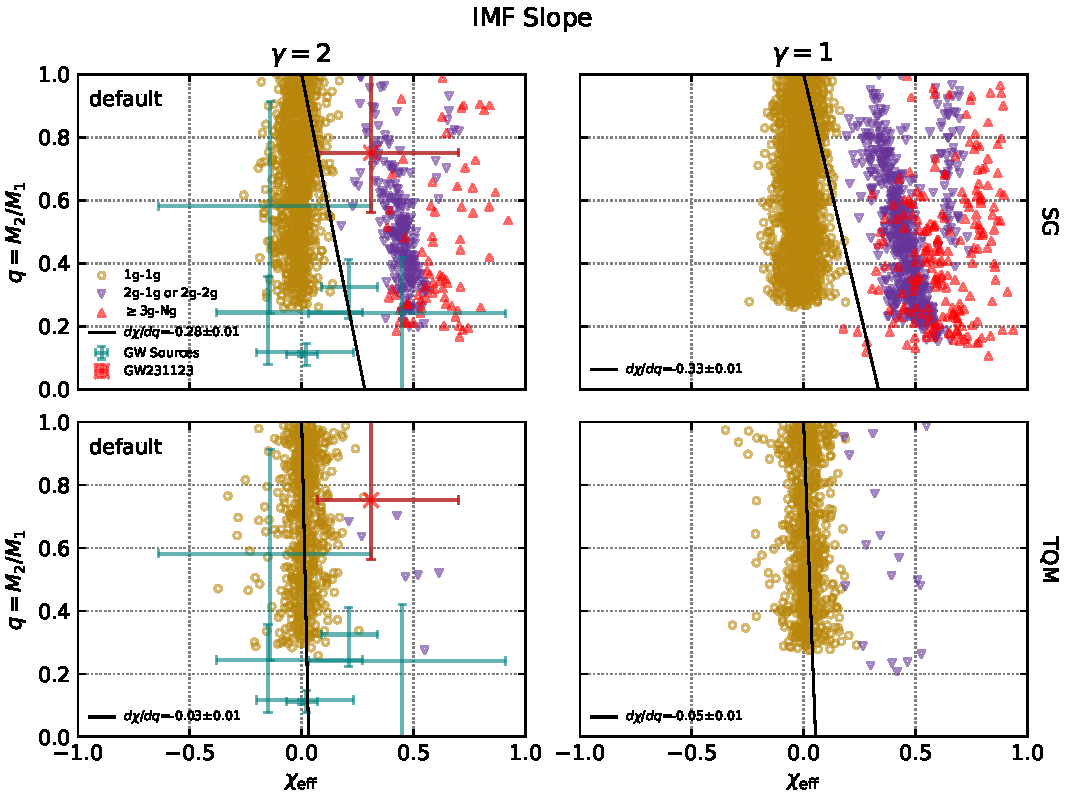
\includegraphics[width=\textwidth]{ch_qxeff_figs/p2_default_imf.pdf}
    \caption[Mass ratio ($q$) distribution as a function of effective spin ($\Xeff$)]{\textbf{Mass ratio ($q$) distribution as a function of $\Xeff$}.
    \textit{Top left:} results from our default setup for a \citet{SirkoGoodman03} disk with BH mass distribution power-law index $\gamma=2$, run \code{sg_default}.
    Gold points represent 1g-1g mergers (see text).
    Inverted purple triangles indicate either 2g-1g or 2g-2g mergers.
    Red triangles indicate $\geq$3g-Ng mergers.
    The solid and dashed lines are fit through ($\Xeff,q)=(0,1)$ and entire and $\geq$2g populations, respectively.
    Teal points with error bars are a representative sample of GW sources chosen to avoid cluttering and provide context for our results: GW190412, GW190521, GW190814, GW200115\_042309, GW200208\_222617, GW200210\_092254.
    The red orange data point with an ``x" represents GW231123.
    \textit{Bottom left:} default setup for a \citet{ThompsonQuataertMurray05} disk, run \code{tqm_default}.
    \textit{Right column:} same as SG and TQM defaults but with shallower IMF index of $\gamma=1$ that increases the probability for high-mass BH.
    Each experiment was performed for 100 galaxies.
    See Table~\ref{tab:run-parameters} for setup parameters and Table~\ref{tab:popstats} for population statistics.}
    \label{fig:default-imf}
\end{figure}

We show the final masses as a function of radius in the left column and time in the right column in  \Fig{fig:default-radius-time}.
In an SG disk (top row), mergers between all generations occur beyond $3\times10^3\,\Rg$, though 1g-1g mergers dominate this region.
As migration torques drive the embedded population inwards, a reduced torque at $\lesssim 10^{3}\,\Rg$ causes a traffic jam as they approach the trap set at $\sim 700\,\Rg$ \citep[also the vertical dashed line]{Bellovary+16}.
For our relatively short-lived default $\sim 0.5$Myr disk, most hierarchical mergers occur in this 'swamp' outside of the trap .
The dense inner disk population here as a result of migration and disk capture, drives the majority of $\geq$2g mergers and produces all remnants with mass $>90\,\Msun$, reinforcing the importance of traps in SG disks for producing BH with masses in the upper mass gap.
The circularization, migration, binary formation, and binary hardening processes take roughly $\sim 0.2$ Myr at which point 1g mergers occur,
consistent with realignment timescales of inclined binaries at migration traps  \citep{Gilbaum+25}.
After $\sim 0.25$Myr, 2g mergers appear, and $\geq$3g mergers start around $\sim 0.33$ Myr.
In each population, the final mass attainable increases with time.

In a TQM disk (bottom row of \Fig{fig:default-radius-time}) torques from radiative feedback combined with low disk opacity cause outward migration towards the disk edge at $5\times10^4\,\Rg$, while inside $10^3\,\Rg$, the torques are more balanced, leading to mergers down to $10^2\,\Rg$.
The TQM disk produces a burst of mergers in the first 0.25 Myr from BH on initially nearly circular orbits.
Then, the rate settles to a steady-state sustained by BH captured from the NSC by the disk.
The much weaker migration torques in TQM disks are unable to concentrate BH as densely as SG disks near migration traps suppressing hierarchical mergers to 3g remnants up to $\sim70\,\Msun$.

\begin{figure}[htbp]
    \centering
    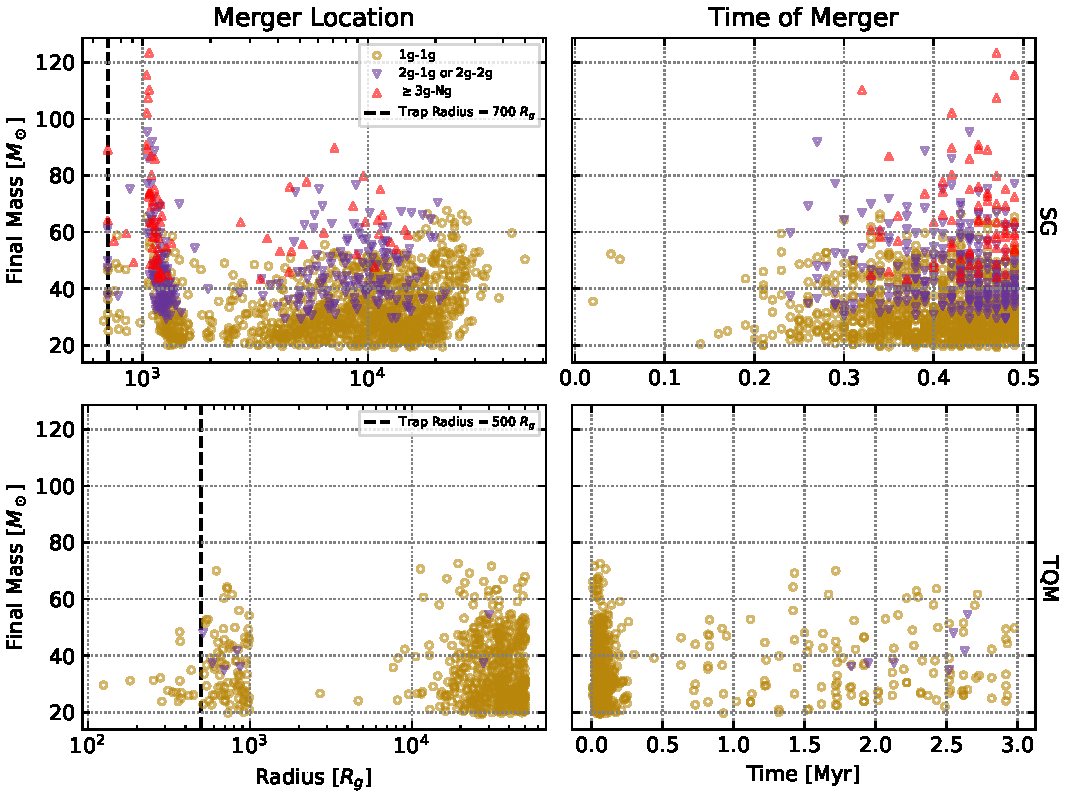
\includegraphics[width=\textwidth]{ch_qxeff_figs/p2_default_radius_time.pdf}
    \caption[Final masses of merger remnants vs. radius and time]{Final masses of merger remnants versus radius (left column) and time (right column) in SG disks (top row) and TQM disks (bottom row).
    Strong migration torques and traps in SG disks near $10^3\,\Rg$ accelerate hierarchical mergers whereas weaker torques in the TQM disk cause traps to be less important leading to a maximum of 3g remnants and lower masses.
    SG disks take $\sim0.2$ Myr to regularly produce 1g mergers with 2g mergers starting at 0.25 Myr and 3g+ mergers at 0.33 Myr, while final mass increases steadily with time and reaches $\sim 120\,\Msun$.
    TQM disks quickly merge the initial embedded BH population in the first 0.25 Myr and reach a steady state as the disk captures more BH.
    The mass range of remnants stays relatively even between 20 and 70 $\Msun$ throughout time.
    Markers are as in \Fig{fig:default-imf}.}
    \label{fig:default-radius-time}
\end{figure}

\begin{figure}
    \centering
    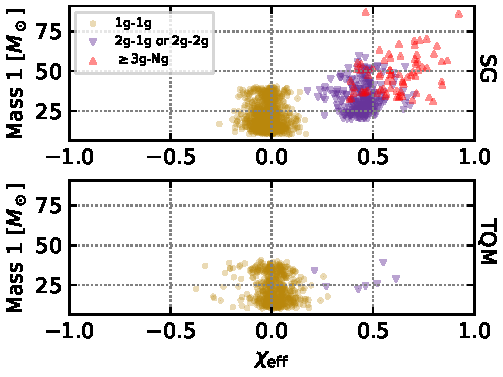
\includegraphics[width=\textwidth]{ch_qxeff_figs/p2_default_mass_v_chieff.pdf}
    \caption[Primary mass vs. $\Xeff$]{\textbf{Primary Mass vs. $\Xeff$.}
    Hierarchical mergers drive primary masses higher and produce mergers with larger values of $\Xeff$.
    Markers are as in \Fig{fig:default-imf}.}
    \label{fig:default-primarymass-xeff}
\end{figure}

Fig.~\ref{fig:default-primarymass-xeff} shows the primary mass of mergers as a function $\Xeff$.
Hierarchical mergers drive up the primary mass of subsequent events which tend to have larger $\Xeff$.
In high generation mergers whose primaries are more likely to have higher mass, randomly oriented spins of companions have less effect on $\Xeff$ since the primaries are remnants that have inherited their spin from the orbital angular momentum of their progenitor BBH, and we have restricted BBH to form with angular momenta aligned with the disk in this setup.

Below we explore the effects of a series of parameters on the intrinsic $q$--$\Xeff$ distributions produced by galaxies hosting a SG or TQM AGN disk model.


\subsubsection{Changing the Mass Function}
First, we test the effect of flattening the BH initial mass function (IMF) by changing the power-law index from a steeper $\gamma=2$ (our default) to $\gamma=1$ (\code{nsc_imf_powerlaw_index} in \mcfacts).
NSCs may have a shallower-than-Salpeter IMF, and indeed a shallow IMF is observed in our own Galactic nucleus \citep[][]{Lu+2013}.

The top right panel of \Fig{fig:default-imf} shows the results from run \code{sg_g1} and is qualitatively similar to $\sgdefault$.
We see the same population islands: a 1g merger population centered on $\Xeff \sim 0$, as well as hierarchical populations at larger $\Xeff$.
However, given a shallower mass function or equivalently a heavier IMF, the typical mass ratio shifts to smaller values, as expected (see Table~\ref{tab:popstats}).
Thus, among the 1g-1g population we can see that the population is dispersed away from $q \sim 1$, evening out the slight tapering seen in the top left panel were $\gamma=2$.
From Table~\ref{tab:popstats}, among 1g mergers $\barq$ drops slightly from $\barq$(1g)$=0.67\pm0.19$ from \code{sg_default} to $\barq$(1g)$=0.63\pm0.21$ in \code{sg_g1} with double the number of mergers, while $\barXeff$(1g) remains the same ($-0.02\pm0.05$ vs. $-0.01\pm0.06$ here).
Among higher generation mergers, visually there is a slight smearing out in both $q,\Xeff$ with the large $q$ region filling in.
Although $\barq,\barXeff$ remain similar to the default within the margins of error for both hierarchical populations, the shallower IMF produces double the number of hierarchical mergers overall and a factor three more mergers of $\geq$3g (see Table~\ref{tab:popstats}).

The slope of the line measuring the anti-correlation decreases significantly from $d\chi/dq=-0.28\pm0.01$ to $d\chi/dq=-0.33\pm0.01$ with shallower IMF.
The change in slope seems mainly driven by the ability for more hierarchical mergers to form, given the larger Hill radius of heavier BH, which increases the likelihood of BBH formation.

As we flatten the BH IMF from $\gamma=2$ in the $\tqmdefault$ setup to $\gamma=1$ for setup \code{tqm_g1}, we do not see any visual difference comparing the two panels in the bottom row in \Fig{fig:default-imf}.
The 1g population shifts slightly down to $\barq({\rm 1g})=0.65\pm0.23$ while $\barXeff$ is identical despite 10\% more mergers.
The 2g population keeps the same $\barq$(2g) but doubling the number of events and increasing the number of low $q$ mergers drives $\barXeff$(2g) to $0.37\pm0.12$.
As for $\gamma=2$, zero $\geq$3g mergers occurred.
The line fit slope does not significantly change between $\tqmdefault$ and \code{tqm_g1}.

For denser disks like SG, hierarchical mergers occur more readily as we flatten the mass function, since migration speed depends linearly on the mass \citep{McKernan+25-mcfactsI}.
The general increase in number of large $\Xeff$ hierarchical events of $\geq$3g can most easily be seen in the steepening of the line fit to the overall population.
Notably, the only appreciable change occurs for $q$ of 2g mergers when changing IMF slope in low density, low torque disks like TQM.


\subsubsection{Accretion Disk Lifetime}
Next, we explore changes in the disk lifetime from our default models.
We consider SG disk lifetime spanning $\tauAGN=[0.25,0.75]$ Myr.
The less dense TQM disk model spans $\tauAGN=[2.5,5]$ Myr.
These adjustments are made by changing \code{timestep_num} according to \code{timestep_duration_yr} (default $10^4\,$yr).

The top row of \Fig{fig:time} shows the results for a SG disk with $\tauAGN=0.25\,$Myr (left, \code{sg_t0p25}) 0.5 Myr (center, $\sgdefault$), and 0.75 Myr (right, \code{sg_t0p75}).
Decreasing $\tauAGN$ decreases the number of 1g and produces a single 2g merger since few BH on eccentric orbits are able to circularize, migrate, form binaries, and merge in such a short $\tauAGN$.
Increasing $\tauAGN$ does not significantly change the population features, however the increased time allows $\geq$3g mergers to fill in the low $q$ and high $\Xeff$ (bottom right) corner of the space.
The island in the upper right region is populated by mergers of BBH where both components are high generations and of similar mass and therefore have spins near the natal value of $\Xeff \sim 0.7$ for merger remnants.

The bottom row of \Fig{fig:time} shows the results for a TQM disk with $\tauAGN=2.5$ Myr (left, \code{tqm_t2p5}) 3 Myr (center, $\tqmdefault$), and 5 Myr (right, \code{tqm_t5}).
Both 1g and 2g populations look very similar except for a slight increase in the number of 2g mergers and some 1g mergers with more negative $\Xeff$ when $\tauAGN=0.75$ Myr.
This latter feature is caused by eccentric BH drastically spinning down during the long circularization process required for this model, but there are no statistically significant changes to any of the diagnostic quantities that are not attributable to low numbers (see Table.~\ref{tab:popstats}).

In SG disks, $\tauAGN$ greatly affects the slope of the anti-correlation even when we exclude the case when $\tauAGN=0.25$ Myr due to the lack of mergers.
Increasing $\tauAGN$ from 0.5 Myr to 0.75 Myr moves fit from $d\chi/dq=-0.28\pm0.01$ to $-0.59\pm0.01$, caused by five times more 2g mergers and ten times more $\geq$3g mergers.
This overall steepening primarily points to a correlation between $\tauAGN$ and the number of hierarchical mergers, especially between high generation progenitors.


\begin{figure}[htbp]
    \centering
    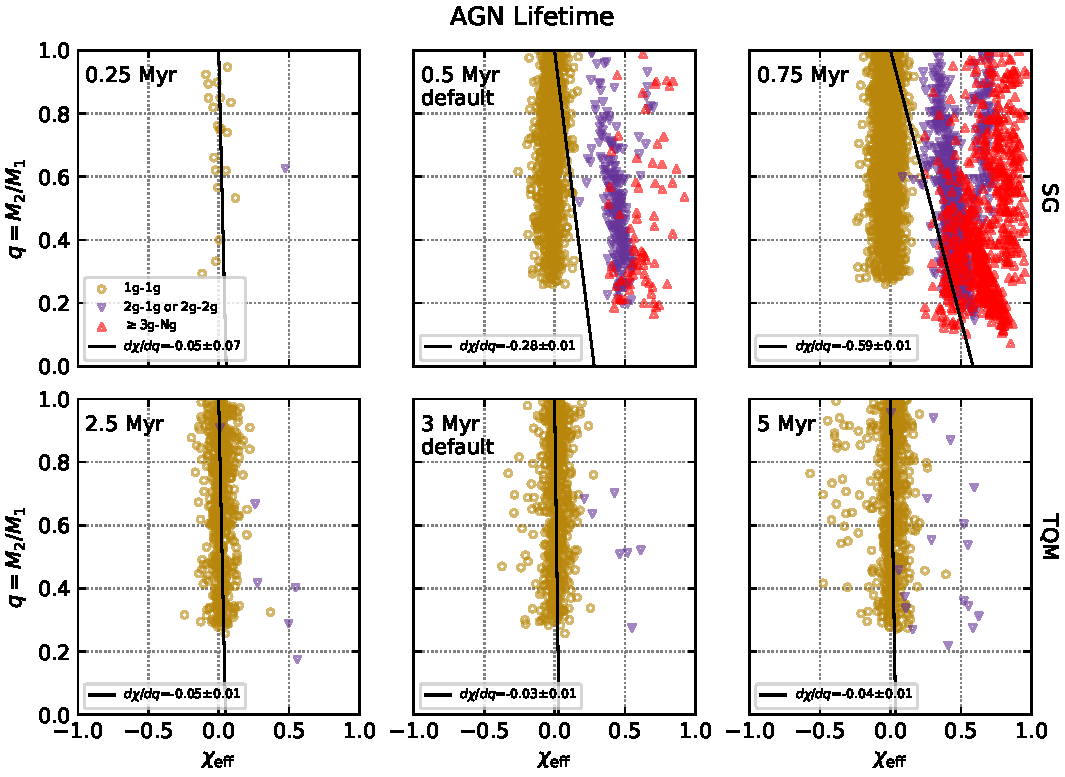
\includegraphics[width=\textwidth]{ch_qxeff_figs/p2_time.pdf}
    \caption[Varying the disk lifetime]{\textbf{Varying the disk lifetime.}
    \textit{Top row:} SG disk setups with $\tauAGN=[0.25,0.5,0.75]$ Myr.
    \textit{Bottom row:} TQM disk setups with $\tauAGN=2.5$, 3, and 5 Myr.
    The anti-correlation steepens with lifetime in dense SG disks as more hierarchical mergers with large $\Xeff$ occur, but $\tauAGN$ has little impact on low density TQM disks.
    Markers are as in \Fig{fig:default-imf}.
    See Table~\ref{tab:run-parameters} for unique setup parameters and Table~\ref{tab:popstats} for population statistics.}
    \label{fig:time}
\end{figure}

Fig.~\ref{fig:time-mass} shows the history of mergers for the runs shown in Fig.~\ref{fig:time}.
As $\tauAGN$ increases, an SG disk steadily produces higher masses via hierarchical mergers.
The $\geq$3g population builds masses up to 100$\,\Msun$ in 0.5 Myr and 200$\,\Msun$ after 0.75 Myr due to saturation at the migration traps.
In contrast, a TQM disk does not produce increasingly massive remnants via hierarchical mergers with longer lifetime.
Not shown here, the behavior in TQM disks continues as long as 10 Myr.

\begin{figure}[htbp]
    \centering
    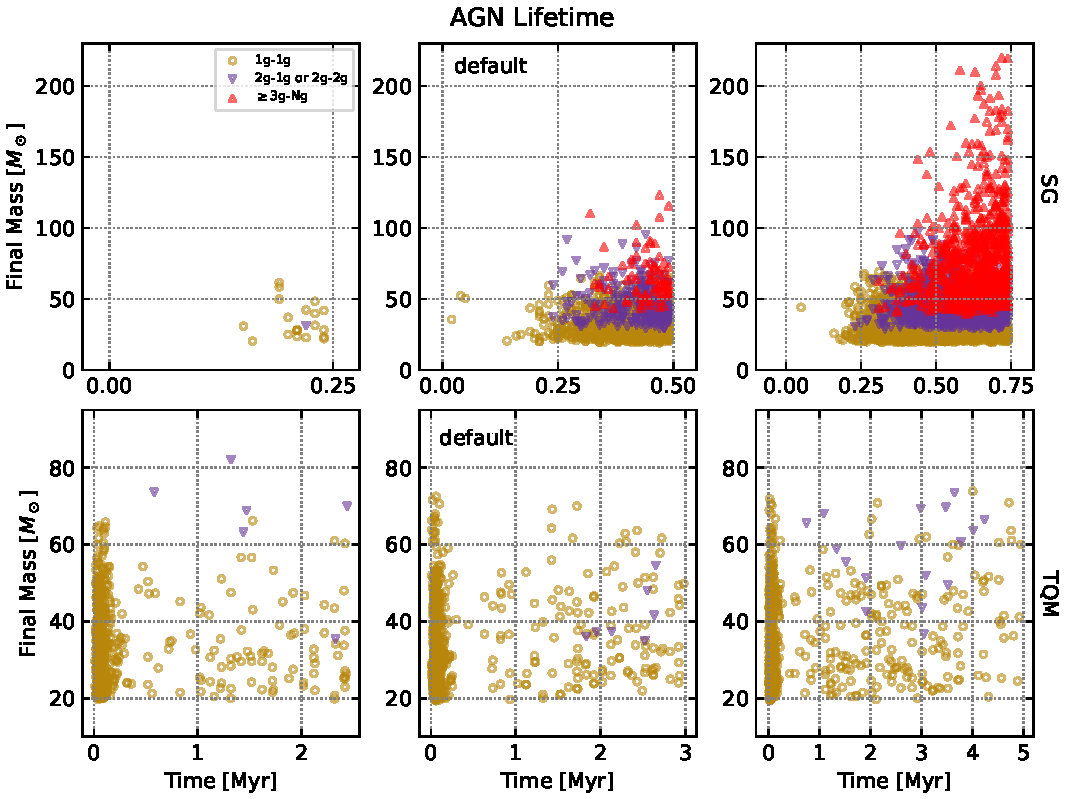
\includegraphics[width=\textwidth]{ch_qxeff_figs/p2_time_final_mass.pdf}
    \caption[Merger remnant mass versus disk lifetime]{\textbf{Merger remnant mass versus disk lifetime.}
    \textit{Top row:} SG disk setups with $\tauAGN=$ 0.25, 0.5, and 0.75 Myr.
    \textit{Bottom row:} TQM disk setups with $\tauAGN=2.5$, 3, and 5 Myr.
    Hierarchical mergers drive up the mass of remnants in SG disks with increased lifetime, whereas TQM disks quickly merge BH on near circular orbits but low migration rates suppresses subsequent interactions to increase remnant masses beyond $\sim80\,\Msun$.
    Markers are as in \Fig{fig:default-imf}.
    See Table~\ref{tab:run-parameters} for unique setup parameters and Table~\ref{tab:popstats} for population statistics.}
    \label{fig:time-mass}
\end{figure}

\subsubsection{Accretion Disk Radius}
Next, we vary the radial extent of each disk model to $R_{\rm out}=2\times10^4$ and $7\times10^4$ $\Rg$ by changing \code{disk_radius_outer}, which affects the initial number of BH in the disk.
\Fig{fig:radius} shows the relevant results.

Smaller disks have a smaller cross section with the NSC and will naturally result in a reduction in the BH merger rate.
This is reflected in the SG setup with $R_{\rm out} = 2\times10^4\,\Rg$ (top left, \code{sg_r2e4}).
Note the number of mergers \emph{also} decreases with larger disk size (top right, \code{sg_r7e4}).
In a slightly larger disk, we do not add significantly more BH.
This is because our default BH radial density function has a power-law break at $R=5 \times 10^{4}r_{g}$, with a steeper power-law index outside ($-2.5$ compared to inside $-7/4$).
As a result, even though the disk is larger, we add proportionally fewer BH and so the average spacing of BH over the range $[\code{disk_radius_inner, disk_radius_outer}]$ must \emph{increase} in our model, thus driving down the average rate.

The line fit for mergers produced in a smaller disk (\code{sg_r2e4}) \emph{increases} to $d\chi/dq=-0.45\pm0.02$ due to a more equal number of mergers in the 1g and $\geq$2g populations as compared to \sgdefault.
A larger disk in \code{sg_r7e4} disk produces a similar slope to \sgdefault\ since the number of events in each population decreased proportionally.

The already low number of mergers in the TQM disk decreases further with a smaller disk radius (bottom left, \code{tqm_r2e4}).
While the SG model saw a \emph{decrease} in mergers for larger disks, the TQM model sees a constant number of mergers when $R_{\rm out}=7\times10^4\Rg$ (bottom right, \code{tqm_r7e4}), due to more room for out-migrating BH due to thermal torques in the low opacity outer disk.

Statistical measures for 1g mergers in the TQM models do not significantly change, but the low number of hierarchical mergers causes ($\barq$(1g), $\barXeff$(1g)) to fluctuate from ($0.71\pm0.17, 0.43\pm0.09$) in \code{tqm_r2e4} to ($0.55\pm0.14, 0.44\pm0.08$) in \tqmdefault\ and ($0.65\pm0.20, 0.36\pm0.09$) in \code{tqm_r7e4}.
This has a strong influence on the measured slope which decreases as radius increases $d\chi/dq=[-0.13\pm0.02, -0.03\pm0.01, -0.05\pm0.01]$.


\begin{figure}[htbp]
    \centering
    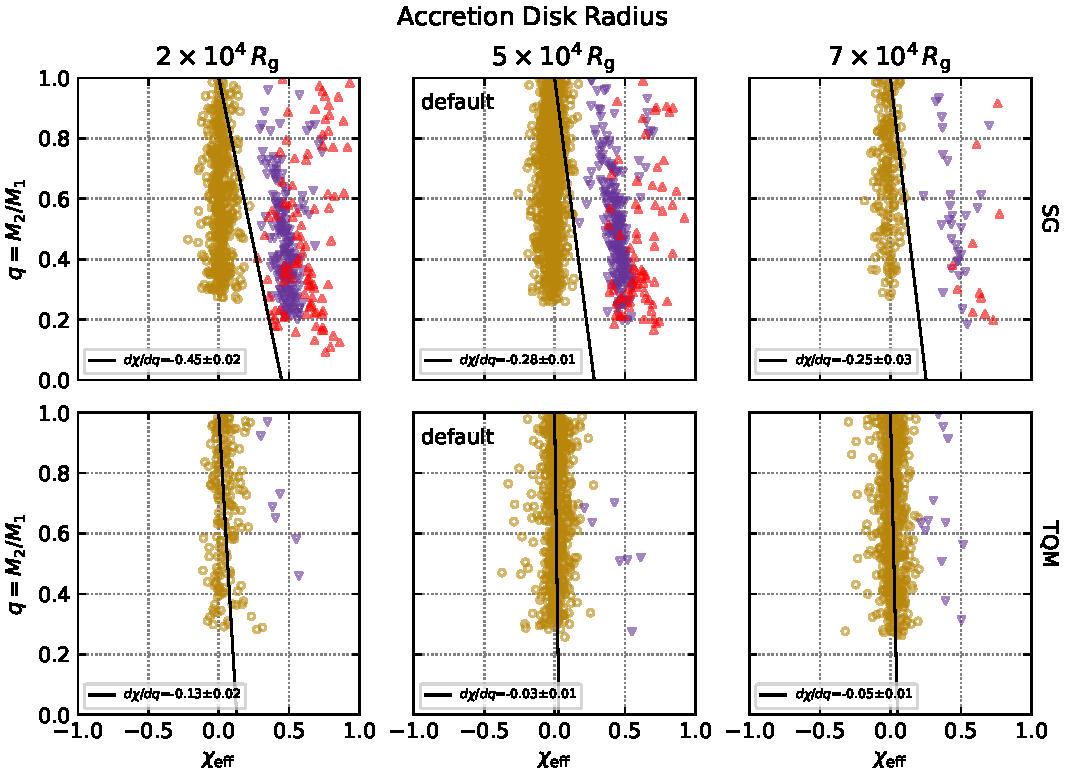
\includegraphics[width=\textwidth]{ch_qxeff_figs/p2_radius.pdf}
    \caption[Varying disk radius]{\textbf{Varying disk radius.}
    SG and TQM disks with radii $r = (2\times 10^{4}, 5\times 10^{4},\,10^{5})\ R_{\rm g}$.
    Both decreases and increases in disk radius result in fewer mergers.
    Model name left-to-right, top-to-bottom: \code{sg_r2e4}, \code{sg_default}, \code{sg_r7e4}, \code{tqm_r2e4}, \code{tqm_default}, and \code{tqm_r7e4}.
    Markers are as in \Fig{fig:default-imf}.
    See Table~\ref{tab:run-parameters} for unique setup parameters and Table~\ref{tab:popstats} for population statistics.}
    \label{fig:radius}
\end{figure}


Fig.~\ref{fig:radius-mass} shows final masses of the mergers as a function of merger location for the corresponding runs shown in Fig.~\ref{fig:radius}.
The trap at $700\,\Rg$ and migration slowdown at $10^3\,\Rg$ produce the majority of hierarchical mergers and high mass remnants in the SG disk, while the slow migration rate in the TQM disk reduces the traps' effectiveness.

For an SG disk, decreasing the radius to $2\times10^4\,\Rg$ produces roughly half the number of mergers (750) versus the default (1412) with radius set to $5\times10^4\,\Rg$, while increasing the radius to $7\times10^4\,\Rg$ significantly reduces the number (214).
As outlined above, average initial separations between BH increase, suppressing e.g. the importance of traps for a default  $\tauAGN = 0.5$ Myr.
An increase to $\tauAGN =0.6$ Myr, yields more time to migrate, producing 489 mergers and the hierarchical population reemerges near the trap.

Changing the disk size in a TQM model produces slightly different behavior for our choices of radii.
Like SG disk, smaller TQM disks overlap with less of the NSC, but the low inner disk opacity reduces the effectiveness of migration and traps and produces only 194 mergers relative to the default size that produces 615 mergers.
By contrast, the higher opacity at large radii in TQM disks drives migration to compensate for the effect of increased separation between BH in large disks described above and produces 614 mergers with the same disk lifetime.

\begin{figure}[htbp]
    \centering
    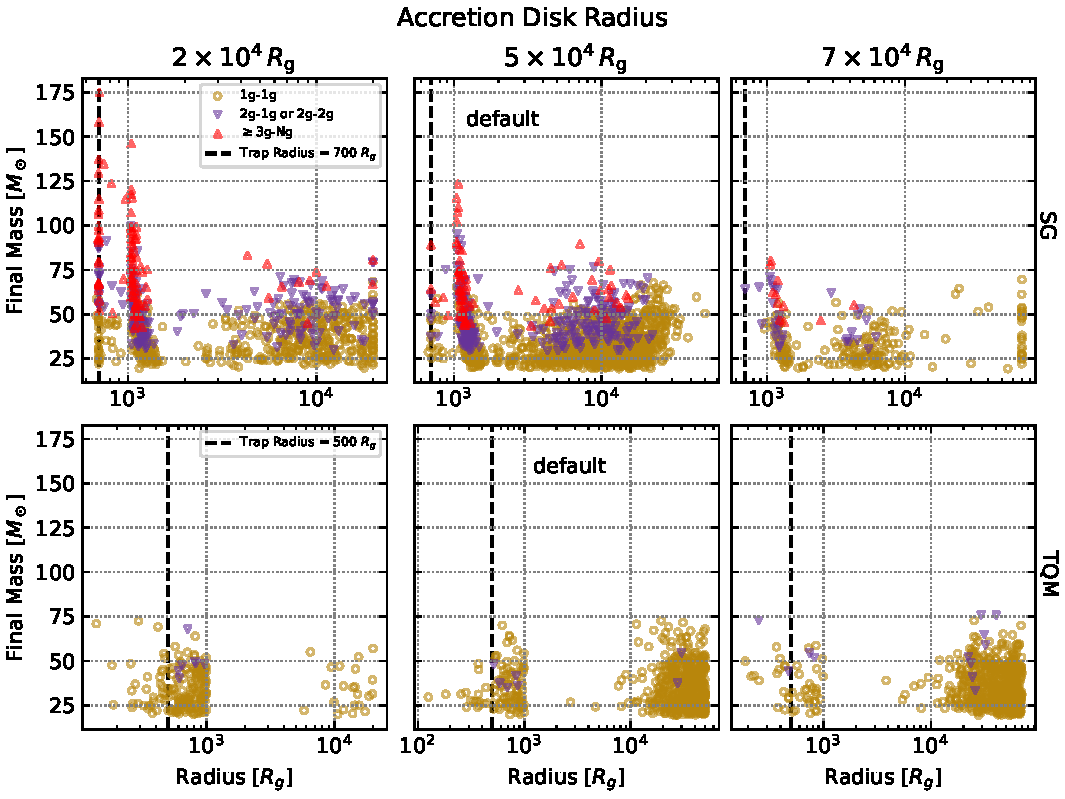
\includegraphics[width=\textwidth]{ch_qxeff_figs/p2_radius_final_mass.pdf}
    \caption[Merger remnant mass vs. disk radius]{\textbf{Merger remnant mass versus disk radius.} Left column shows outer disk radii set to $2\times10^4\,\Rg$ compared to the default $5\times10^4\,\Rg$ in the center column, and $7\times10^4\,\Rg$ in the right column.
    SG disks produces less mergers with both changes for SG (top row).
    Shrinking a TQM (bottom row) disk also produces less mergers, but extending this disk includes more of the optically thick outskirts that drives migration in this model so the number of mergers is the same as the default case.
    Markers are as in \Fig{fig:default-imf}.}
    \label{fig:radius-mass}
\end{figure}

\subsubsection{Initial Black Hole Spin Magnitude Distribution}
Here we explore the influence of the allowed initial BH spin magnitude distribution.
We vary the width of the initial Gaussian distribution between $\sigma_\chi=[0.02,0.2]$ to reflect a range of natal spin magnitudes by setting the parameter \code{nsc_bh_spin_dist_sigma}.

In \Fig{fig:spin} we see each test produces the usual population islands as the default setups.
For SG disks, no significant change occurs in $\barq$ for any of the generational subpopulations (top left: \code{sg_s0p02} and top right: \code{sg_s0p20}).
However, we see the spread in $\Xeff$ for the 1g population is greatly impacted and grows as the spin width increases from $\sigma_\chi= 0.02$ to $0.20$.
The standard deviation on $\barXeff$(1g) reflects this trend, tightening to $-0.01\pm0.02$ when $\sigma_\chi = 0.02$ and broadening to $-0.02\pm0.10$ when $\sigma_\chi = 0.20$.
While no statistically significant change is seen in $\barXeff$ for the hierarchical populations, tighter initial distributions of spin magnitude (smaller $\sigma_\chi$) cause their islands to be more concentrated, whereas a larger $\sigma_\chi$ increases their scatter.

The TQM model shows similar behavior as the SG disk when varying $\sigma_\chi$ (bottom left: \code{tqm_s0p02} and bottom right: \code{tqm_s0p20}).
The $\barq$ of 1g mergers stays the same, but the variance on $\barXeff$ is correlated with increasing $\sigma_\chi$.
For $\sigma_\chi=0.02,\ 0.10,\ 0.20$, $\barXeff$(1g)$=0.01\pm0.04,\ 0.01\pm0.07,\ 0.02\pm0.12$, respectively, but the number of hierarchical mergers is too low to make any robust claims regarding their means.

If the detected population has a component with a wide distribution of $\Xeff$ centered around $\Xeff=0$, for the AGN channel this implies 1g BH in NSCs have a broad range of initial spin values, possibly reflecting details of star formation and/or gas accretion in the galactic nucleus.
If the measured effective spins follow narrow distributions (both centered on $\Xeff \sim 0$ and at higher $\Xeff$), then 1g BH in NSCs are likely born with a very narrow range of spins (close to zero).
Constraints from future BBH catalogs (O4 and O5) on the width of the $\Xeff$ distribution will allow us to test models of BH birth and evolution in galactic nuclei.

Changing $\sigma_\chi$ does not appear to significantly impact the expectation values for either disk model.
But the intrinsic distributions in spin are likely $\sigma_\chi \leq 0.2$ in SG models since the standard deviation on $\Xeff$ for the 1g population resulting from this setting extends to negative $\Xeff$ about as far as \citet[]{Callister+21} report is observed.
TQM models produce similar results for 1g mergers, but the number of hierarchical events remains limited.

\begin{figure}[htbp]
    \centering
    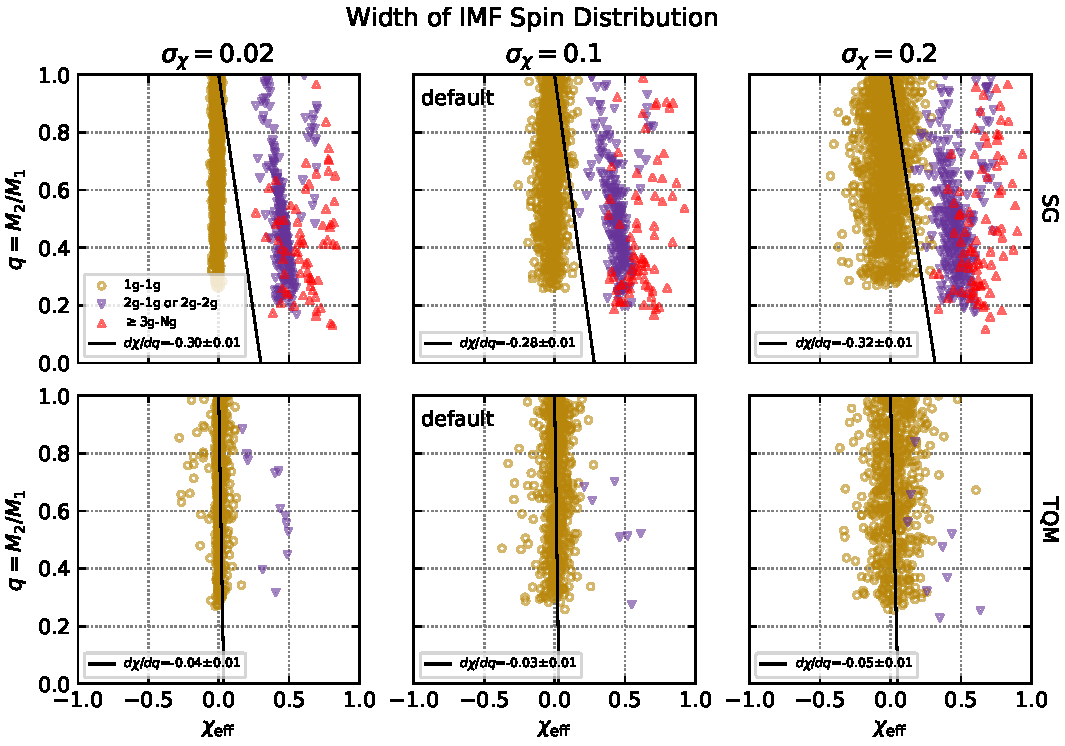
\includegraphics[width=\textwidth]{ch_qxeff_figs/p2_spin.pdf}
    \caption[Exploring impact of initial black hole spin magnitude distribution]{\textbf{Varying the width of the Gaussian distribution for initial BH spin magnitudes.}
    \textit{Top left:} SG disk with spin magnitude distribution $\sigma_\chi = 0.02$ (\code{sg_0p02}).
    \textit{Top-center:} Default SG disk with $\sigma_\chi=0.1$ (\code{sg_default}).
    \textit{Top-right:} SG disk with $\sigma_\chi = 0.2$ (\code{sg_0p2}).
    \textit{Bottom row:} Same as top row but for a TQM disk model (\code{tqm_0p02}, \code{tqm_default}, \code{tqm_0p2}).
    Narrower (wider) spin magnitude distributions primarily affect the 1g population by narrowing (widening) the distribution in $\Xeff$.
    Markers are as in \Fig{fig:default-imf}.
    See Table~\ref{tab:run-parameters} for unique setup parameters and Table~\ref{tab:popstats} for population statistics.}
    \label{fig:spin}
\end{figure}



% Retrograde binaries
\subsubsection{Impact of Retrograde Binaries}
\label{sec:retro-results}
We now relax the default requirement for prograde BBH only and test a retrograde fraction $\fret=0.1,0.5.$ Retrograde BBH orbit retrograde around their center of mass, but prograde around the SMBH.
Control this parameter in \mcfacts with \code{fraction_bin_retro}.
A perfectly symmetric  distribution in $\Xeff$ around $\Xeff \sim 0$ consistent with is a $d\chi/dq$ slope of zero.
This should by definition be the case for the $\fret=0.5$ (see \Fig{fig:retro}, where $d\chi/dq=0.0\pm0.01$).

The top row of \Fig{fig:retro} shows the results for increasing $\fret$ in a SG disk.
In each case, the 1g population remains symmetric about $\Xeff=0$ without change from the fiducial setup.
When $\vec{L}_{\rm bin}<0$ and $\chi_{1,2}>0$ for both BH, $\Xeff$ will be negative.
This is also true when $q$ is sufficiently small and the more massive BH's spin is pointed opposite to $\vec{L}_{\rm bin}$.
Increasing  $\fret=0$ (top left, $\sgdefault$) to $\fret=0.1$ (top center, \code{sg_fr0p1}), primarily affects the mean effective spin of the hierarchical population, and we see a handful of these appear on the left side of the plot for $\fret=0.1$.
For all hierarchical mergers, $\barXeff$ decreases with increasing $\fret$ as more negative $\Xeff$ events occur, but the standard deviation increases drastically as a result.
For $\fret=0$, $\barXeff$(2g)$=0.44\pm0.08$, but when $\fret=0.1$, $\barXeff$(2g)$=0.38\pm0.27$.
The $\geq$3g population sees even greater uncertainty increases with $\barXeff(\geq$3g)$=0.61\pm0.13$ changing to $0.44\pm0.42$.

The change in $d\chi/dq$ reflects these shifts by drastically shifting towards negative $\Xeff$, flattening from $-0.28\pm0.01$ to $-0.24\pm0.01$.
Even a few negative $\Xeff$ hierarchical events skew the measurement.

Increasing $\fret \rightarrow 0.5$ continues this trend (top right, \code{sg_fr0p5}).
The symmetry about $\Xeff=0$ we have seen in the 1g population now extends to the hierarchical mergers.
Effectively $\fret=0.5$ is equivalent to a gas-free hierarchical merger environment.
Since half of the hierarchical mergers now have $\Xeff<0$, the mean expectation value shifts to $\barXeff$(2g)$=-0.02\pm0.46$.
There are no underlying differences to the hierarchical mergers compared to $\sgdefault$ (top left), which can be seen by taking the absolute value of the effective spin before calculating the mean $\overline{|\Xeff|}$(2g)$=0.45\pm0.08$ -- consistent with $\barXeff=0.44\pm0.08$ seen in \sgdefault.
Similar behavior is reflected in the $\geq$3g population with $\barXeff(\geq$3g)$=0.06\pm0.63$ vs.
$\overline{|\Xeff|}(\geq$3g)$=0.61\pm0.14$ when $\fret=0.5$ (see Table.~\ref{tab:popstats}).

The symmetry in the hierarchical population flattens the slope to $d\chi/dq=-0.24\pm0.01$ when $\fret=0.1$ and $0.00\pm0.01$ when $\fret=0.5$.
Retrograde BBH are not expected to form this frequently in an AGN disk, but as one allows for more to occur by increasing $\fret$, the number of negative $\Xeff$ events increases, and the measured slope flattens.

The bottom row of \Fig{fig:retro} shows the results for the TQM model.
As in the SG model, changing $\fret$ to 0.1 (bottom center, \code{tqm_fr0p1}) produces some $\Xeff<0$ hierarchical mergers, and $\fret=0.5$ (bottom right, \code{tqm_fr0p5}) increases this number further, while $\barXeff({\rm 2g})$ decreases to $0.17\pm0.37$ for $\fret=0.1$ and to $-0.07\pm0.40$ when $\fret=0.5$.
These shifts lead to decreasing slopes: $d\chi/dq=[-0.28\pm0.01, -0.24\pm0.01, 0.00\pm0.01]$.
Though this disk model is plagued by low number statistics for hierarchical mergers, a small $\fret$ still greatly affects the measurement of $d\chi/dq$.

\begin{figure}[htbp]
    \centering
    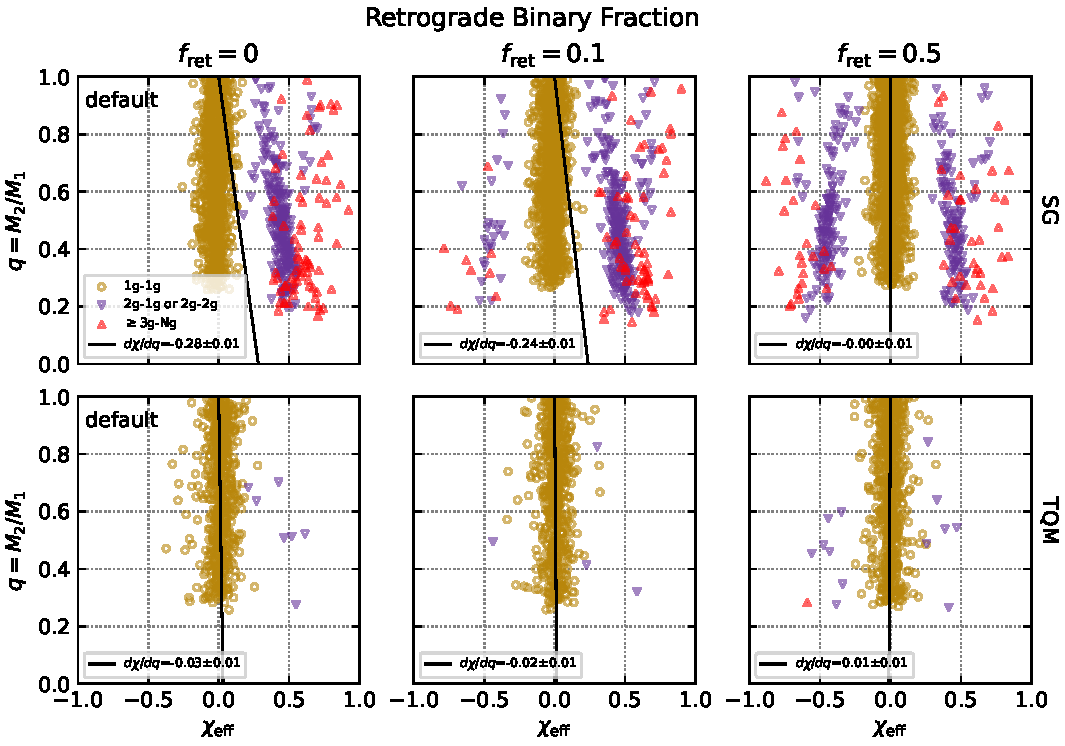
\includegraphics[width=\textwidth]{ch_qxeff_figs/p2_retro.pdf}
    \caption[Varying the retrograde binary black hole fraction]{\textbf{Varying the retrograde BBH fraction.}
    \textit{Left column:} Default SG and TQM disk setups where no retrograde BBH form ($\fret=0$, \code{sg_default}).
    \textit{Center column:}  Retrograde fraction is $\fret=0.1$ (\code{sg_fr0p1}).
    \textit{Right column:} Half of BBH are retrograde ($\fret=0.5$)  (\code{sg_fr0p5}).
    Increasing allowed retrograde fraction splits the hierarchical population to negative $\Xeff$ and flattens the slopes of the anti-correlation for SG-like disks.
    The TQM model (bottom row, \code{tqm_default}, \code{tqm_fr0p1}, \code{tqm_fr0p5}) reflects this behavior but the hierarchical population still suffers from low numbers.
    Markers are as in \Fig{fig:default-imf}.
    See Table~\ref{tab:run-parameters} for unique setup parameters and Table~\ref{tab:popstats} for population statistics.}
    \label{fig:retro}
\end{figure}




\subsubsection{Black Hole Orbital Eccentricity}

In this section we explore the effects of changing the maximum initial orbital eccentricity $\emax$ of the embedded BH.
Migration does not occur unless a BH has been circularized, defined when $e_{\rm crit}\leq0.01$.
For eccentric prograde BH, mass accretion is retrograde, spinning down embedded BH.
Thus, more eccentric BH that spend a longer time circularizing experience more spin-down before they can migrate and form BBH.
Control this parameter in \mcfacts with \code{disk_bh_orb_ecc_max_init}.

\subsubsubsection{SG disk: $\emax= 0.1, 0.3, 0.5$}

\Fig{fig:ecc-sg} shows the results from a BH population with orbits constrained to be more circular ($\emax=0.1$, left panel, \code{sg_e0p1}) or more eccentric ($\emax=0.5$, right panel, \code{sg_e0p5}).
Starting from lower $\emax$, the 1g population becomes saturated across the entire range of possible mass ratios, but no change occurs to the populations expectation values for $q$ or $\Xeff$.
The same is true for the 2g and $\geq$3g populations.
The slope does slightly steepen from $d\chi/dq=-0.28\pm0.01$ to $-0.35\pm0.01$ due to the relative increase in number of hierarchical mergers.
Conversely, the number of mergers decreases in each group for a larger $\emax$, and the suppression of hierarchical mergers flattens the slope to $-0.19\pm0.03$.

Given a fixed $\tauAGN$, starting from orbits with a lower $\emax$ reduces time spent circularizing, jump starts the migration process, and increases the pool of BH available to form BBH at early times.
Since more BH spend a longer time participating in mergers, the $\geq$3g hierarchical merger population is able to reach lower mass ratios and higher effective spins.

\begin{figure}[htbp]
    \centering
    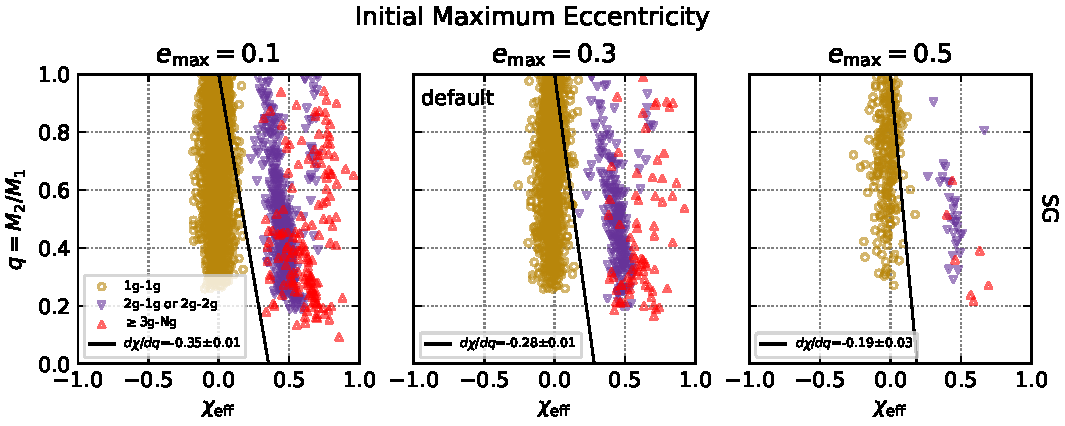
\includegraphics[width=\textwidth]{ch_qxeff_figs/p2_ecc_sg.pdf}
    \caption[Varying the initial maximum orbital eccentricity]{\textbf{Varying the initial maximum orbital eccentricity.}
    SG disk with NSC initial eccentricity capped at $e_{\rm max}=0.1$ (left, \code{sg_e0p1}), 0.3 (center, \code{sg_default}), and 0.5 (right, \code{sg_0p5}).
    The number of mergers is inversely proportional to initial eccentricity.
    Markers are as in \Fig{fig:default-imf}.
    See Table~\ref{tab:run-parameters} for unique setup parameters and Table~\ref{tab:popstats} for population statistics.}
    \label{fig:ecc-sg}
\end{figure}

\subsubsubsection{SG disk with thermal distribution: $\emax=0.7$}

A thermal NSC is either one that has not had substantial recent AGN cooling activity or one that had sufficient time between active phases for dynamical encounters to erase the circularization caused by previous AGN activity and has median orbital eccentricity $\overline{e} \sim 0.7$.
\Fig{fig:ecc-sg-thermal} shows an SG accretion disk interacting with a thermal BH population for $\tauAGN=0.5$ Myr (center panel, \code{sg_e0p7}) suppresses almost all mergers.
However, if $\tauAGN=0.7$ Myr (right panel, \code{sg_e0p7_t0p75}) there is sufficient time to damp embedded BH orbits to broadly match \sgdefault\ results.
However, the 1g population qualitatively shifts towards negative $\Xeff$ --- though less so quantitatively (left panel: $\barXeff$(1g)$= -0.01\pm0.05$, right panel: $-0.02\pm0.06$) --- since accretion-driven spin down during a lengthy circularization period leads to initially highly eccentric BHs forming BBH with spins pointing opposite to the binary orbital angular momentum.
This can be tested in LVK O4.



\begin{figure}[htbp]
    \centering
    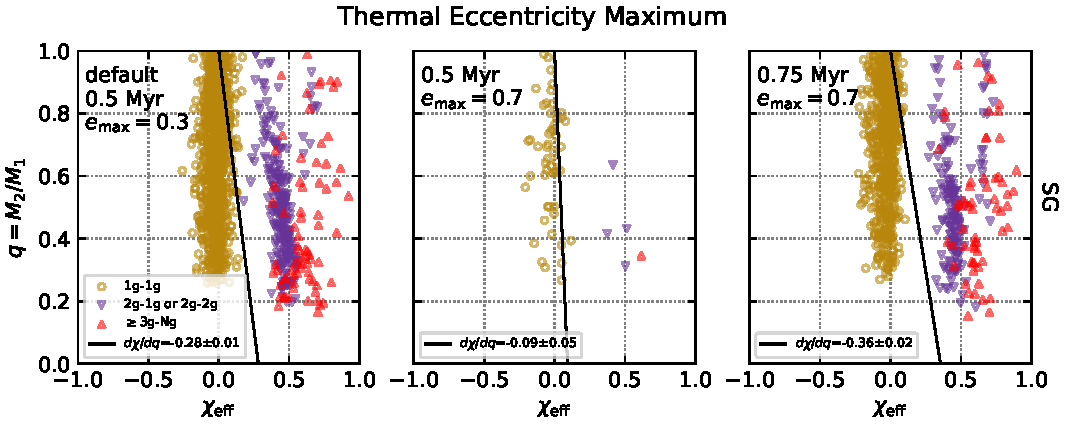
\includegraphics[width=\textwidth]{ch_qxeff_figs/p2_ecc_sg_thermal.pdf}
    \caption[Initial thermal population for varying lifetimes]{\textbf{Thermal Population with varying lifetimes.}
    \textit{Left:} Default SG disk with $\emax=0.3$ (\code{sg_default}).
    \textit{Center:} SG disk interacting with a thermal NSC with $\emax=0.7$ (\code{sg_e0p7}).
    \textit{Right:} Thermal NSC with SG disk lifetime increased to $\tauAGN=0.75$ Myr (\code{sg_e0p7_t0p75}).
    A more eccentric initial BH population takes longer to circularize which increases the time to produce mergers.
    Markers are as in \Fig{fig:default-imf}.
    See Table~\ref{tab:run-parameters} for unique setup parameters and Table~\ref{tab:popstats} for population statistics.}
    \label{fig:ecc-sg-thermal}
\end{figure}

\subsubsubsection{TQM disk: $\emax = 0.015, 0.05, 0.1$}

The default TQM setup uses a lower default eccentricity maximum $\emax = 0.05$ which we now vary between $\emax=0.015,0.1$.
Examining \Fig{fig:ecc-tqm} shows that for $\emax=0.1$ (right panel, \code{tqm_e0p1}) the hierarchical merger population is unchanged, and the 1g merger population drops by half.
Even this small $\emax$ almost significantly suppresses mergers.
Conversely, when $\emax = 0.015$ (left panel, \code{tqm_e0p015})---only $\Delta e = 0.005$ above our eccentricity criterion for treating orbits as circular---we see for the first time in any TQM set-up, a distribution of hierarchical mergers that appears remotely similar to the SG model default.
The 1g population is densely concentrated about $\Xeff=0$ with $\barXeff({\rm 1g})=0.02\pm0.06$ over the range of mass ratios $0.25 \lesssim q \leq 1$ with $\barq({\rm 1g})=0.68\pm0.21$.
The hierarchical population is finally large enough for more robust expectation values of $\barXeff({\rm 2g})=0.35\pm0.16$ and $\barq({\rm 2g})=0.59\pm0.19$.
However, there are over 60 times as many 1g mergers, and the anti-correlation's slope is flat at $d\chi/dq=-0.05\pm0.00$.

\begin{figure}[htbp]
    \centering
    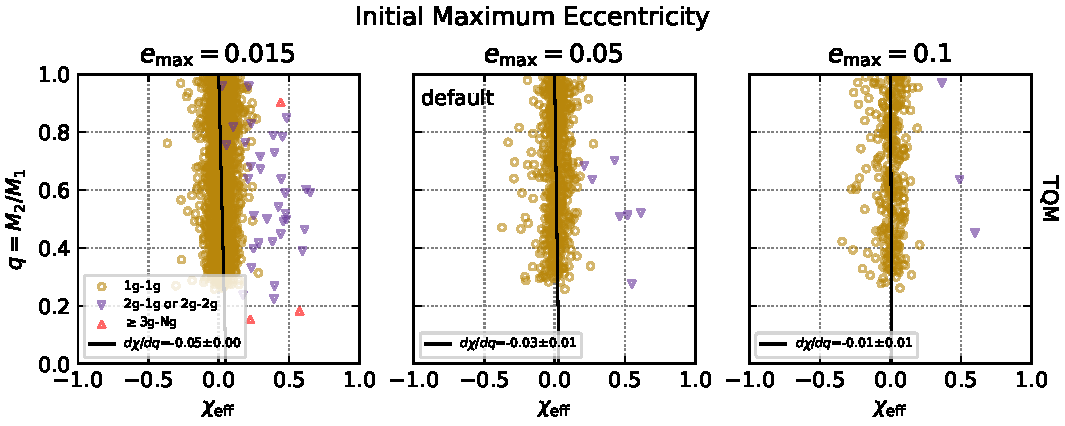
\includegraphics[width=\textwidth]{ch_qxeff_figs/p2_ecc_tqm.pdf}
    \caption[Varying the initial maximum orbital eccentricity]{\textbf{Varying the initial maximum orbital eccentricity.}
    TQM disk with NSC initial eccentricity capped at $e_{\rm max}=0.015$ (left \code{tqm_e0p015}), 0.05 (center \code{tqm_default}), and 0.1 (right, \code{tqm_e0p1}).
    The number of mergers is inversely proportional to initial eccentricity, and an extremely low eccentricity is required for the TQM model to produce an appreciable number of hierarchical mergers as opposed to the SG model.
    Markers are as in \Fig{fig:default-imf}.
    See Table~\ref{tab:run-parameters} for unique setup parameters and Table~\ref{tab:popstats} for population statistics.}
    \label{fig:ecc-tqm}
\end{figure}


\subsubsubsection{TQM disk with circular orbits: $\emax=0$}

The TQM model has been unable to produce any significant number of hierarchical mergers with a slightly eccentric initial NSC.
Here we explore how $\tauAGN$ affects the $q$--$\Xeff$ plane, when the NSC starts from circularized orbits.

\Fig{fig:ecc-tqm-circular} shows the results from evolving the circular NSC ($\emax=0$) in a TQM disk for $\tauAGN=[1,3]$ Myr compared with our default setup.
The only difference between the 3 Myr run (center panel, \code{tqm_e0}) and the default setup (right panel) is the initial maximum eccentricity, yet already within 1 Myr the $\geq$2g population begins to populate more similar to \code{tqm_e0p015}.
At 1 Myr, the 1g population is still highly concentrated in effective spin, expected at $\barXeff({\rm 1g})=0.03\pm0.08$ and $\barq({\rm 1g})=0.68\pm0.21$.
The mean effective spin for 2g hierarchical events is $\barXeff({\rm 2g})=0.53\pm0.12$, and the mean mass ratio is $\barq({\rm 2g})=0.63\pm0.20$.
The hierarchical population does not affect anti-correlation's slope because there are almost 4000 1g mergers compared to the 23 2g mergers, causing the slope to flatten $d\chi/dq=-0.07\pm0.00$.
After 3 Myr the number of 2g mergers increases to 89, and 3 $\geq$3g mergers occurred---the most in any TQM model.
$\barXeff$(2g) moves to $0.45\pm0.14$ and is slightly larger at $0.71\pm0.03$ for $\geq$3g.
The additional 69 $\geq$2g mergers and only $\sim$150 additional 1g mergers slightly shifts the slope to $d\chi/dq=-0.09\pm0.00$

By skipping the damping process for eccentric orbits, a circularized population of BH interacting within a TQM-like disk can immediately migrate, form binaries, and merge.
By jump-starting the merger process, then number of hierarchical mergers produced within 1 Myr is four times larger than when the BH have even a tiny initial eccentricity ($\emax=0.015$).
Though 3 Myr increases the hierarchical population, they primarily occur near $R=2\times10^4\,\Rg$, and far fewer higher generation ($\geq 3$g) mergers occur compared to SG disks which benefit from the trap.
This behavior suggests TQM-like disks quickly exhaust the embedded 1g population, and are unable to continue merging higher generation BBH, because of slow (inefficient) migration in the outer disk.
Thus, low density disks with dynamically cooled populations could contribute to the 1g population without significantly contributing to high mass BBH mergers.

\begin{figure}[htbp]
    \centering
    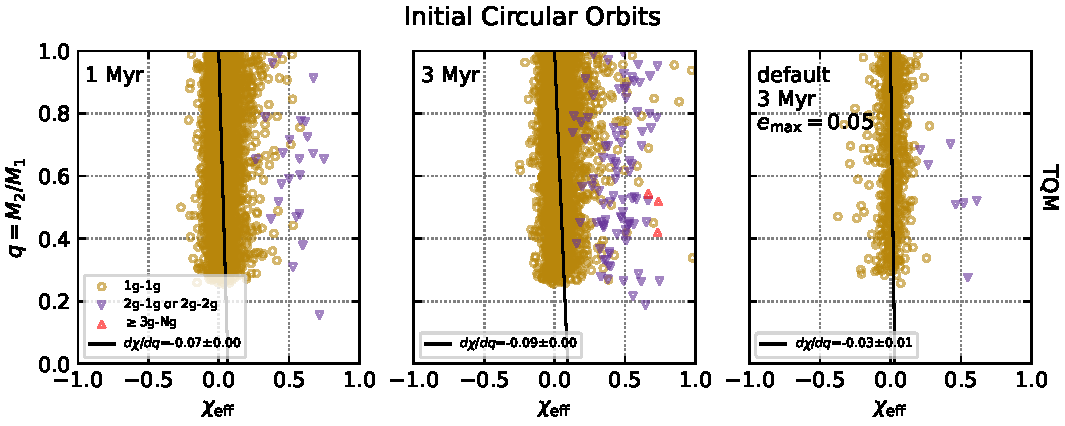
\includegraphics[width=\textwidth]{ch_qxeff_figs/p2_ecc_tqm_circular.pdf}
    \caption[Initially circular orbits for varying lifetimes]{\textbf{Initially circular orbits with varying AGN lifetimes.}
    \textit{Left:} TQM disk evolved for $\tauAGN=1$ Myr (\code{tqm_e0_t1}).
    \textit{Center:} Setup same as \tqmdefault but with circular BH orbits ($\tauAGN=3$ Myr; \code{tqm_e0}).
    \textit{Right:} Default TQM setup where $\tauAGN=3$ Myr and initial eccentricity is capped at $\emax=0.05$ (\code{tqm_default}).
    Markers are as in \Fig{fig:default-imf}.
    See Table~\ref{tab:run-parameters} for unique setup parameters and Table~\ref{tab:popstats} for population statistics.}
    \label{fig:ecc-tqm-circular}
\end{figure}


\subsection{Discussion}
\label{sec:discussion-qxeff}
One of the most intriguing results to emerge from the LVK O3 GW results was an apparent anti-correlation between BBH mass ratio ($q=M_{2}/M_{1}$) and the BBH effective spin \citep[$\Xeff$,][]{Callister+21}.
At first glance this seems unexpected from most channels.
The AGN channel was recognized as a possible source of such an anti-correlation simply because: a) the primary BH ($M_{1}$) in BBH should spend longer in the AGN disk and so, b) primary BH ($M_{1}$) spins should be biased towards alignment with the orbital angular momentum of the disk (and the BBH) \citep[e.g.][]{McKernan+22:q-Xeff,Santini+23, DittmannDempseyLi24}.
Here we have demonstrated the form of the $q$--$\Xeff$ parameter space distribution as a function of different disk and model choices for the AGN channel.

First, and most importantly, our default choice of a SG disk run for 0.5 Myr with a $\gamma=2$ IMF seems to be a reasonable fit to the observed $q$--$\Xeff$ distribution (see \Fig{fig:default-imf} top left panel).
\citet{Callister+21} find an overall anti-correlation fit of $d\chi/dq \sim -0.46^{+0.29}_{-0.28}$ for their distribution when they exclude GW190814.
However, when they \emph{include} GW190814, they find $d\chi/dq=-0.28^{+0.31}_{-0.28}$ which matches $d\chi/dq=-0.28\pm0.01$ from our default SG model.
This highlights an important point: GW190814 is difficult to reproduce commonly in any other channel, however in AGN (depending on choice of IMF) such low $q \sim 0.1$ events can occur at the few percent level \citep{Secunda+19, McKernan+20b,TagawaHaimanKocsis20}.

Second, it is clear that the AGN channel produces islands of population in $q$--$\Xeff$ parameter space.
Evidently the 1g mergers tend (at least in dense SG-like disks) to be concentrated around $\Xeff \sim 0$.
Higher generation hierarchical mergers ($\geq$2g) tend to live in islands at higher $\Xeff$.
Indeed, the structure, location, and density of these population islands is what drives the $d\chi/dq$ in the AGN channel.
For example, a steep IMF ($\gamma=2$) tends to drive $q \sim 0.5$ mergers, whereas a flatter IMF ($\gamma=1$) drives lower q mergers and drives the average ($d\chi/dq$) slope to more negative values (compare Fig.~\ref{fig:default-imf} top panels).
Future LVK results (e.g.
from O4) can constrain the presence (or not) of such islands.

Third, while higher-density SG disks can reproduce the $d\chi/dq$ correlation, we find that low-density AGN disk models can only approach this correlation if the initial BH population has been dynamically cooled (compare e.g.
Fig.~\ref{fig:default-imf} bottom panels and Fig.~\ref{fig:ecc-tqm-circular}).
Indeed some level of dynamical cooling is also preferred in denser SG-like disks (see Fig.~\ref{fig:ecc-sg}).
Only very small initial eccentricities for BH embedded in TQM-like disk models can reproduce the observed $d\chi/dq$ anti-correlation  \citep{Callister+21}.
Lower surface density disk models like TQM take longer to circularize and migrate embedded BH, leading to lower merger rates than SG-like models.
If we extend the disk lifetime ($\tauAGN$), we can drive a higher BBH merger rate, but at the expense of spin down due to retrograde accretion from the gas disk for an initially eccentric population (see Fig.~\ref{fig:time} bottom panels).
So it is unlikely that low density disks are a significant contributor to the observed LVK rate among higher mass mergers unless their initial populations are dynamically cold (low $e$).

Fourth, as the width of BH initial spin distribution $\sigma_\chi$ increases, the width of the islands in $q$--$\Xeff$ parameter space increases (see gold, purple and red populations in  Fig.~\ref{fig:spin}).
Larger values of $\sigma_\chi$ lead to a larger weighting of the 1g population to negative $\Xeff$.
We constrain $\sigma_\chi \leq 0.2$ in the AGN channel from LVK observations.

Fifth, the gradient ($d\chi/dq$) in the AGN channel is also driven by the ratio ($\fret$) of retrograde/prograde BBH mergers.
For $\fret=[0,0.1,5]$, the gradient $d\chi/dq=[-0.28\pm0.01,\ -0.24\pm0.01,\ 0.00\pm0.01]$ for our default model in an SG disk.
As \citet{Callister+21} find $d\chi/dq = -0.28^{+0.31}_{-0.28}$ from O3, a low value of $\fret$ is preferred, but we cannot exclude $\fret \sim 0.5$.
The value of $\fret$ for mergers in AGN disks remains an unsolved problem.
The change in separation between BBH formation and merger is 6-7 orders of magnitude and the details of what happens during hardening in AGN remain unclear.
BBH formation via GW capture in gas disks can be either prograde or retrograde \citep[e.g.][]{DeLaurentiis+23,Whitehead+24,QianLiLai24}.
However, retrograde BBH may have their eccentricity pumped \citep{Li+22-bbh-evo,Calcino+23}, and may therefore harden quickly towards merger.
However, there is much debate as to whether retrograde BBH are preferentially separated as their eccentricity is pumped \citep{Wang+21}, or whether they are flipped to prograde due to dynamical encounters \citep{Samsing+22,McKernanFord24}.
The slope of the ($d\chi/dq$) anti-correlation that emerges from larger data sets (O4, O5) will allow us to directly test models of the retrograde fraction of BBH in the AGN channel.

Sixth, disk size impacts both the overall rate of BBH mergers and the $q$--$\Xeff$ distribution (see \Fig{fig:radius}).
A small average disk size generates a plausible $q$--$\Xeff$ distribution but a far lower merger rate.

Seventh, more massive primaries tend to produce mergers with higher $\Xeff$ (see Fig.~\ref{fig:default-primarymass-xeff}) since they are more likely to be 2g or $\geq$3g and thus had their spins aligned with the disk.

\subsection{Conclusion}
The observed LVK BBH rate of $\mathcal{R} \sim 25\,{\rm Gpc}^{-3} {\rm yr}^{-1}$ \citep{Abbott+23-O3b} originates from a variety of formation channels, potentially including some fraction from AGN.
From \citet{McKernan+25-mcfactsI} the merger rates for our default SG disk is $\mathcal{R} \sim 20\,{\rm Gpc}^{-3} \rm{yr}^{-1}$, whereas the default TQM rate is only $\mathcal{R} \sim 0.1\,{\rm Gpc}^{-3} \rm{yr}^{-1}$.
SG-like AGN are efficient at making IMBH, driving low $q$ and high $\Xeff$ mergers, whereas low density/opacity, TQM-like disks are far less efficient producers of hierarchical merger events.
As demonstrated, features in the $q$--$\Xeff$ plane due to AGN channel BBH mergers depend strongly on the disk model, so LVK O4 results will allow us to constrain possible AGN disk models.

 

\begin{sidewaystable}
\centering
{\footnotesize
\begin{tabular}{r|c|c|ccc|ccc|ccc}
\hline\hline
Run & Fig. & $d\chi/dq$ & \multicolumn{3}{c}{1g-1g Mergers} & \multicolumn{3}{c}{2g-[1,2]g Mergers} & \multicolumn{3}{c}{$\geq$3g-Ng Mergers} \\
 &  &  & N & $\barq$ & $\barXeff$ & N & $\barq$ & $\barXeff$ & N & $\barq$ & $\barXeff$ \\
    \hline
    \code{sg_default} & \ref{fig:default-imf},\ref{fig:default-radius-time},\ref{fig:default-primarymass-xeff} & $-0.28\pm0.01$ & 1093 & $ 0.67\pm0.19$ & $-0.02\pm0.05$ & 244 & $ 0.51\pm0.18$ & $ 0.44\pm0.08$ & 73 & $ 0.45\pm0.22$ & $ 0.61\pm0.13$ \\
    \code{tqm_default} & \ref{fig:default-imf},\ref{fig:default-radius-time},\ref{fig:default-primarymass-xeff} & $-0.03\pm0.01$ & 606 & $ 0.68\pm0.20$ & $ 0.01\pm0.07$ & 7 & $ 0.55\pm0.14$ & $ 0.44\pm0.14$ & 0 & --- & --- \\
    \hline
    \code{sg_g1} & \ref{fig:default-imf} & $-0.33\pm0.01$ & 1925 & $ 0.63\pm0.21$ & $-0.01\pm0.06$ & 556 & $ 0.50\pm0.21$ & $ 0.46\pm0.10$ & 207 & $ 0.44\pm0.22$ & $ 0.63\pm0.16$ \\
    \code{tqm_g1} & \ref{fig:default-imf} & $-0.05\pm0.01$ & 683 & $ 0.65\pm0.23$ & $ 0.01\pm0.07$ & 18 & $ 0.55\pm0.27$ & $ 0.37\pm0.12$ & 0 & --- & --- \\
    \hline
    \code{sg_t0p25} & \ref{fig:time},\ref{fig:time-mass} & $-0.05\pm0.07$ & 20 & $ 0.70\pm0.19$ & $-0.00\pm0.06$ & 1 & $ 0.63\pm0.00$ & $ 0.47\pm0.00$ & 0 & --- & --- \\
    \code{sg_t0p75} & \ref{fig:time},\ref{fig:time-mass} & $-0.59\pm0.01$ & 2246 & $ 0.69\pm0.19$ & $-0.02\pm0.05$ & 1004 & $ 0.51\pm0.18$ & $ 0.47\pm0.09$ & 756 & $ 0.44\pm0.22$ & $ 0.67\pm0.15$ \\
    \code{tqm_t2p5} & \ref{fig:time},\ref{fig:time-mass} & $-0.05\pm0.01$ & 572 & $ 0.67\pm0.21$ & $ 0.02\pm0.06$ & 6 & $ 0.48\pm0.24$ & $ 0.36\pm0.20$ & 0 & --- & --- \\
    \code{tqm_t5} & \ref{fig:time},\ref{fig:time-mass} & $-0.04\pm0.01$ & 620 & $ 0.67\pm0.21$ & $ 0.00\pm0.10$ & 17 & $ 0.52\pm0.23$ & $ 0.36\pm0.21$ & 0 & --- & --- \\
    \hline
    \code{sg_r2e4} & \ref{fig:radius},\ref{fig:radius-mass} & $-0.45\pm0.02$ & 465 & $ 0.60\pm0.19$ & $ 0.02\pm0.06$ & 187 & $ 0.46\pm0.17$ & $ 0.48\pm0.08$ & 96 & $ 0.47\pm0.25$ & $ 0.62\pm0.15$ \\
    \code{sg_r7e4} & \ref{fig:radius},\ref{fig:radius-mass} & $-0.25\pm0.03$ & 198 & $ 0.70\pm0.19$ & $-0.02\pm0.05$ & 30 & $ 0.54\pm0.20$ & $ 0.45\pm0.10$ & 11 & $ 0.42\pm0.23$ & $ 0.63\pm0.10$ \\
    \code{tqm_r2e4} & \ref{fig:radius},\ref{fig:radius-mass} & $-0.13\pm0.02$ & 185 & $ 0.70\pm0.21$ & $ 0.04\pm0.07$ & 7 & $ 0.71\pm0.17$ & $ 0.43\pm0.09$ & 0 & --- & --- \\
    \code{tqm_r7e4} & \ref{fig:radius},\ref{fig:radius-mass} & $-0.05\pm0.01$ & 600 & $ 0.66\pm0.21$ & $ 0.01\pm0.07$ & 12 & $ 0.65\pm0.20$ & $ 0.36\pm0.09$ & 0 & --- & --- \\
    \hline
    \code{sg_s0p02} & \ref{fig:spin} & $-0.30\pm0.01$ & 1234 & $ 0.68\pm0.20$ & $-0.01\pm0.02$ & 262 & $ 0.50\pm0.19$ & $ 0.46\pm0.07$ & 67 & $ 0.42\pm0.18$ & $ 0.62\pm0.14$ \\
    \code{sg_s0p20} & \ref{fig:spin} & $-0.32\pm0.01$ & 1263 & $ 0.69\pm0.19$ & $-0.02\pm0.10$ & 299 & $ 0.50\pm0.19$ & $ 0.47\pm0.10$ & 87 & $ 0.47\pm0.22$ & $ 0.64\pm0.13$ \\
    \code{tqm_s0p02} & \ref{fig:spin} & $-0.04\pm0.01$ & 595 & $ 0.70\pm0.20$ & $ 0.01\pm0.04$ & 12 & $ 0.61\pm0.17$ & $ 0.37\pm0.12$ & 0 & --- & --- \\
    \code{tqm_s0p20} & \ref{fig:spin} & $-0.05\pm0.01$ & 586 & $ 0.67\pm0.21$ & $ 0.02\pm0.12$ & 9 & $ 0.47\pm0.19$ & $ 0.32\pm0.16$ & 0 & --- & --- \\
    \hline
    \code{sg_fr0p1} & \ref{fig:retro} & $-0.24\pm0.01$ & 1144 & $ 0.68\pm0.19$ & $-0.01\pm0.05$ & 265 & $ 0.50\pm0.19$ & $ 0.38\pm0.27$ & 69 & $ 0.43\pm0.22$ & $ 0.44\pm0.42$ \\
    \code{sg_fr0p5} & \ref{fig:retro} & $0.00\pm0.01$ & 1177 & $ 0.70\pm0.19$ & $ 0.00\pm0.06$ & 255 & $ 0.51\pm0.19$ & $-0.02\pm0.46$ & 61 & $ 0.46\pm0.20$ & $ 0.06\pm0.63$ \\
    \code{tqm_fr0p1} & \ref{fig:retro} & $-0.02\pm0.01$ & 580 & $ 0.67\pm0.21$ & $ 0.01\pm0.07$ & 4 & $ 0.51\pm0.19$ & $ 0.17\pm0.37$ & 0 & --- & --- \\
    \code{tqm_fr0p5} & \ref{fig:retro} & $ 0.01\pm0.01$ & 601 & $ 0.67\pm0.21$ & $0.00\pm0.07$ & 13 & $ 0.50\pm0.15$ & $-0.07\pm0.40$ & 1 & $ 0.28\pm0.00$ & $-0.59\pm0.00$ \\
    \hline
    \code{sg_e0p1} & \ref{fig:ecc-sg} & $-0.35\pm0.01$ & 1778 & $ 0.68\pm0.20$ & $-0.01\pm0.05$ & 464 & $ 0.50\pm0.19$ & $ 0.46\pm0.08$ & 156 & $ 0.45\pm0.22$ & $ 0.62\pm0.14$ \\
    \code{sg_e0p5} & \ref{fig:ecc-sg} & $-0.19\pm0.03$ & 231 & $ 0.71\pm0.17$ & $-0.02\pm0.06$ & 30 & $ 0.53\pm0.14$ & $ 0.44\pm0.07$ & 7 & $ 0.37\pm0.14$ & $ 0.54\pm0.10$ \\
    \code{sg_e0p7} & \ref{fig:ecc-sg-thermal} & $-0.09\pm0.05$ & 51 & $ 0.65\pm0.18$ & $-0.03\pm0.07$ & 4 & $ 0.45\pm0.12$ & $ 0.45\pm0.06$ & 1 & $ 0.35\pm0.00$ & $ 0.62\pm0.00$ \\
    \code{sg_e0p7_t0p75} & \ref{fig:ecc-sg-thermal} & $-0.36\pm0.02$ & 631 & $ 0.71\pm0.18$ & $-0.03\pm0.06$ & 161 & $ 0.52\pm0.18$ & $ 0.46\pm0.09$ & 61 & $ 0.50\pm0.20$ & $ 0.63\pm0.13$ \\
    \hline
    \code{tqm_e0p015} & \ref{fig:ecc-tqm} & $-0.05\pm0.00$ & 2041 & $ 0.68\pm0.21$ & $ 0.02\pm0.06$ & 34 & $ 0.59\pm0.19$ & $ 0.35\pm0.16$ & 3 & $ 0.41\pm0.35$ & $ 0.41\pm0.14$ \\
    \code{tqm_e0p1} & \ref{fig:ecc-tqm} & $-0.01\pm0.01$ & 300 & $ 0.66\pm0.21$ & $ 0.00\pm0.08$ & 3 & $ 0.69\pm0.21$ & $ 0.49\pm0.10$ & 0 & --- & --- \\
    \code{tqm_e0_t1} & \ref{fig:ecc-tqm-circular} & $-0.07\pm0.00$ & 3901 & $ 0.68\pm0.21$ & $ 0.03\pm0.08$ & 23 & $ 0.63\pm0.20$ & $ 0.53\pm0.12$ & 0 & --- & --- \\
    \code{tqm_e0} & \ref{fig:ecc-tqm-circular} & $-0.09\pm0.00$ & 4066 & $ 0.68\pm0.21$ & $ 0.03\pm0.09$ & 89 & $ 0.59\pm0.21$ & $ 0.45\pm0.14$ & 3 & $ 0.49\pm0.05$ & $ 0.71\pm0.03$ \\
\end{tabular}
}
\caption[Statistical estimates of the merger events]{We report the $d\chi/dq$ slope of a line fit to all mergers anchored through the point $(\Xeff,q)=(0,1)$, the number of mergers, the mean mass ratio $\barq$, mean effective spin $\barXeff$, and relevant standard deviations, for 1g-1g, 2g-Ng (2g-1g and 2g-2g), and $\geq$3g-Ng merger events in the associated figure.}
\label{tab:popstats}

\end{sidewaystable}




\clearpage
\resetcounters
\addtocontents{toc}{\protect}
\section{\texorpdfstring{\MakeUppercase{supernova shock breakout from active galactic nuclear accretion disks}}{supernova shock breakout from active galactic nuclear accretion disks}}
\label{sec:sn-hydrodynamics}

\counterwithin{figure}{section}
\counterwithin{table}{section}

\par The models and corresponding results developed in this chapter are currently under review for publication in the \textit{Astrophysical Journal}.
As such, the main text of this chapter is directly informed by the content of that publication.
To cite this chapter, please use Cook et al. (2026a) when possible.

\subsection{Abstract}
\label{sec:motivation-snhydro}
We aim to assess how shocks evolve in the dense stratified medium of AGN disks and understand where the kinetic energy injected by SN explosions from embedded stars is absorbed, or \emph{muffled}, as opposed to where they are able to break free from the disk.
We generate midplane radial profiles using the SG and TQM one-dimensional AGN disk models with the help of the \code{pAGN} code.
We compare the disk pressure as a function of radius to the energy of a standard core-collapse SN ($10^{51}\,{\rm erg}$) to find locations where shock-breakout can occur.
For verification, we evolve three-dimensional hydrodynamic shearing box simulations of disks with Gaussian stratification constructed from select midplane values and inject energy and mass from SNe using the \code{Athena} code to explore several radial and vertical placements.
We find SNe shocks in SG disks around black holes with mass $\Mbh=10^6\,\Msun$ become muffled beyond $R\sim10^6\,\Rs$, and that this muffling radius is inversely proportional to SMBH mass such that the muffling radius moves inward to $R\sim10^2\,\Rs$ for $\Mbh=10^9\,\Msun$.
Around TQM disks, the muffling radius occurs at $R\sim10^6\,\Rs$, independent of $\Mbh$.
We find the largest determining factor for muffling a SN shock is the local scale height of the AGN disk.
In conclusion, we developed a predictive analytic criterion to identify where AGN disks can muffle SNe shocks depending on their density and vertical scale.

% ======================
% ======================

\subsection{Methods}
\label{sec:methods-snhydro}




\citet{MacLowMcCray88} showed repeated SNe from star clusters can inflate superbubbles in disk galaxies.
These bubbles can break free from the disk when the internal mechanical wind luminosity exceeds a characteristic luminosity scale set by local intensive thermodynamic quantities.
Using their formalism, we can analytically compute where SNe are expected (or not expected) to break out from the AGN disk with further implications for observability dependent on the disk opacity.

Whether a SN explosion occurring at an AGN disk's midplane will break free from the disk or be muffled, can be roughly determined by comparing the ram pressure of the SN, or, equivalently, its energy density
\begin{equation}
    \varepsilon_{\rm SN} \equiv \frac{\Esn}{V_{\rm SN}}\ {\rm erg\ cm^{-3}}
\end{equation}
to the gas pressure of the disk at the explosion site
\begin{equation}
    P_D(r) = n k T.
\end{equation}
$\Esn$ is the total kinetic energy released by the SN (typically, $10^{51}$ erg), $V_{\rm SN}$ is the volume bound by the SN shock wave, number density $n$ and temperature $T$ are those of the disk at the SN site given its radius from the SMBH, and $k$ is Boltzmann's constant.
The relative influence of the two is determined by their ratio
\begin{equation}
    \C \equiv \frac{\varepsilon_{\rm SN}}{P_{\rm D}}.
\end{equation}

At early stages of the SN evolution, the shock will remain quasi-spherical.
Its volume after expanding to a radius $\Rsn$ is thus $V_{\rm SN} = (4\pi/3) \Rsn^3$, leading to
\begin{equation}
    \C = \frac{\Esn}{V_{\rm SN}P_{\rm D}} = \frac{3}{4\pi k} \frac{\Esn}{n T R_{\rm SN}^3}.
\end{equation}
We set the SN radius at breakout to be one disk scale height $\Rsn=H$, assume a pure hydrogen gas (proton mass $\mProt$), and substitute the gas volume density $\rho=n\mProt$. The criterion for breakout becomes 
\begin{equation} \label{eqn:C}
    \C = \frac{3\mProt}{4\pi k}\frac{\Esn}{\rho \,T\,H^3}.
\end{equation}
Though the vertical structure is Gaussian, we set $\rho$ and $T$ to the midplane quantities as conservative estimates.

When $\C > 1$, the pressure in the SN shock exceeds the disk's gas pressure, and the SN will break free from the disk.
Since the path of least resistance lies perpendicular to the disk midplane, most of the expansion will be directed along the $z$-direction, temporarily excavating a column of the disk until the disk shear elongates and fills the cavity \citep{Rozyczka+95, Moranchel+21}. 
When $\C < 1$, the SN lacks the pressure to break free from the disk, leading to a \emph{muffled} SN.
Because they do not completely perforate the disk, these SNe impart a significant portion of $\Esn$ as heat into the disk, modifying the local temperature and disk structure.
In fact, \citet{SirkoGoodman03} cite this as a possible mechanism to prevent gravitational collapse in the outer disk.
In the left column of Fig.~\ref{fig:disk-models} we show radial profiles of midplane density, midplane temperature, scale height, and optical depth for SG disks orbiting SMBHs with masses $M_{\rm BH}=\{10^6, 10^7, 10^8, 10^9\}\,\msun$ as calculated with the \code{pAGN} package \citep{Gangardt+24-pAGN}.

For a SN explosion with $\Esn=10^{51}$ erg orbiting a $10^8\,\msun$ SMBH at 1000 Schwarzschild radii $\Rs$ in an SG disk, the midplane temperature, density, and local scale height are $T\sim 10^5$ K, $\rho\sim10^{-9}\ \gcmcube$, and $H \sim 10$ AU, respectively.
We find $\C \sim 2600$, indicating a strong breakout is expected.
Substituting these values into \eq{eqn:C}, we can rewrite $\mathcal{C}$ as a scaling relation

\begin{equation}
    \C \approx 2600 \ \left(\frac{\Esn}{10^{51}\,{\rm erg}} \right) \ \left({\frac{\rho_0}{10^{-9}\,\rm{g\,cm^{-3}}}}\right)^{-1} \
	\left({\frac{T}{10^5\,{\rm K}}}\right)^{-1} \
    \left({\frac{H}{10\,{\rm AU}}}\right)^{-3} \ 
    \exp\left( \frac{z^2}{2H^2}\right)
    \label{eqn:C-parameterized}
\end{equation}
where we have also introduced the midplane density $\rho_0$ and the exponential vertical profile in terms of $H$ to accommodate SNe on inclined orbits (see Sec.~\ref{sec:disk-model} for more details).

\begin{figure}
    \centering
    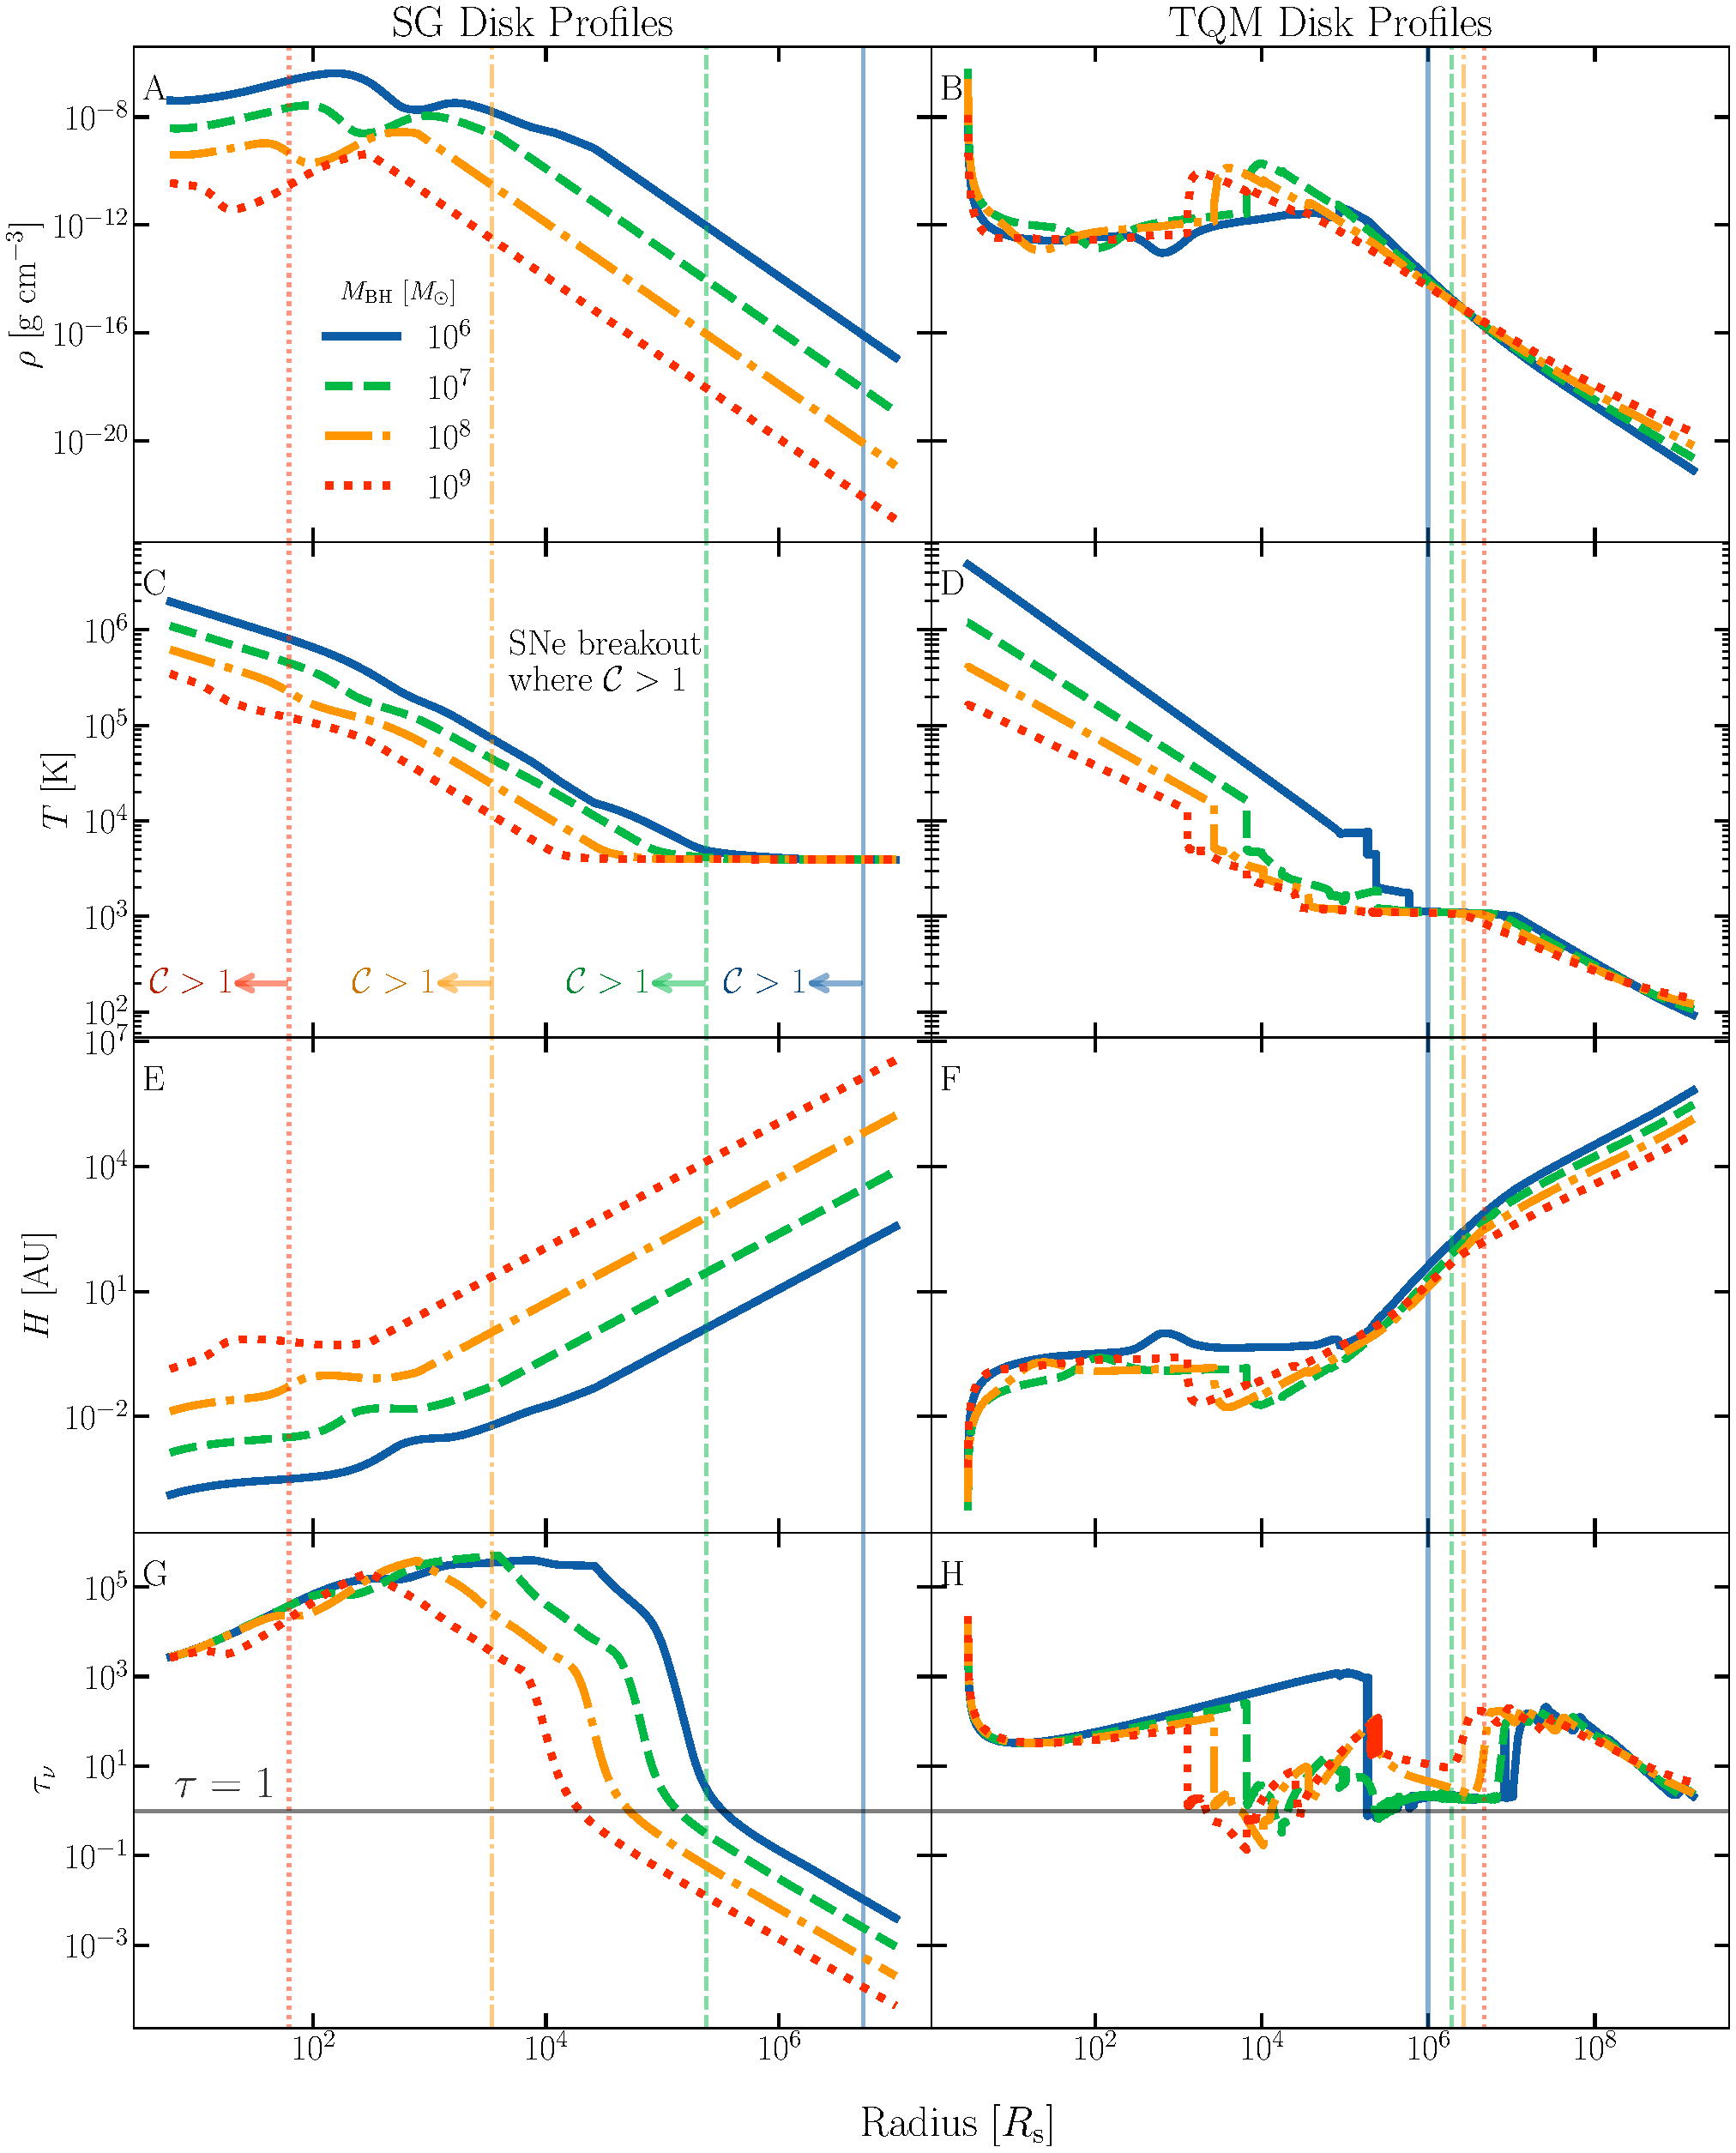
\includegraphics[width=0.9\linewidth]{ch_snhydro_figs/disk_profiles_columns.pdf}
	\caption[Accretion disk midplane models]{\citet[][left column]{SirkoGoodman03} and \citet[][right column]{ThompsonQuataertMurray05} accretion disk models of midplane density (A, B), midplane temperature (C, D), local scale height (E, F), and optical depth (G, H) as functions of radius for disks orbiting various SMBH masses.
    Vertical lines indicate where $\C=1$ for accretion disk models corresponding to SMBH with the same line style.
    In each case, $\C>1$ to the left of these lines.}
    \label{fig:disk-models}
\end{figure}

Profiles for the TQM disk model in the right column of Fig.~\ref{fig:disk-models} tell a different story, resulting in a drastically altered landscape for $\C$, as discussed in \sect{sec:results-snhydro}.
For all SMBH masses, the inner TQM disk is less dense while the opposite is true in the outer torus.
The temperatures are similar to the SG model in the inner disk, but where SG bottoms out at $\sim 4 \times 10^3\,\rm{K}$ and holds that temperature until the disk edge, the TQM model extends down to $100\,\rm{K}$.
The density differences are reflected in the local scale height, which are elevated in the inner regions, while suppressed beyond $R>10^5\,\Rs$.
The optical depths behave much differently, with SG disks typically transitioning from being optically thick to thin at $R=10^5\,\Rs$ whereas TQM remain entirely optically thick except near $R=10^4\,\Rs$ for $\Mbh<10^7\,\msun$.
The vertical lines mark where $\mathcal{C}=1$ for disk models corresponding to the same line styles indicating the SMBH mass.


\subsubsection{Hydrodynamic Models}
\label{sec:hydro}

We test the validity of Eq.\,(\ref{eqn:C-parameterized}) using three-dimensional shearing box hydrodynamic simulations with the publicly available \code{Athena} code, a finite-volume code for compressible hydrodynamics problems \citep{Stone+08, StoneGardiner10}.
The code solves the Riemann problem at each cell interface to determine the flux of quantities over time.
We find the Harten-Lax-van Leer-Einfeldt (HLLE) solver \citep{Einfeldt+91} achieved the most robust numerical stability across the strong shocks we produce and is employed for all our models.

\subsection{Dynamical Equations} \label{sec:dyn-eq}
\code{Athena} solves the equations of motion in the standard Cartesian shearing box approximation in the following form
\begin{align}
    &\ptderiv{\rho} + \Div{\left(\rho\vec{}{v}\right)} = 0
    \label{eqn:cons_mass} \\
    &\ptderiv{\rho \vec{v}} + \Div{\left(\rho \vec{v} : \vec{v}\right)} + \nabla P =
    \rho \Omega_{0}^{2}(2qx{\bf \hat{i}} - z{\bf \hat{k}}) - 2\Omega_{0} {\bf \hat{k}} \times \rho \vec{v}
    \label{eqn:cons_momentum} \\
    &\ptderiv{E} + \Div{\left[\vec{v}\left(E + P\right)\right]} =
    \Omega_{0}^{2}\rho\vec{v} \cdot (2qx{\bf \hat{i}} - z{\bf \hat{k}}).
    \label{eqn:cons_energy}
\end{align}
where $\rho$ is the gas density, $t$ is time, $\vec{v}$ the gas velocity, $P$ is the gas pressure, and $\Omega(r) = (GM_{\rm BH}/r^3)^{1/2}$ is the Keplerian orbital frequency evaluated at the radial location corresponding to the center of the shearing box.
The logarithmic shearing parameter $q_\text{shear}$ is related to the orbital frequency by
\begin{equation}
    q_\text{shear} \equiv -\frac{d\ln\Omega(r)}{d\ln r}.
\end{equation}
We set $q=3/2$ for a Keplerian flow.
The variables $x$, $y$, and $z$ represent the local radial, azimuthal, and vertical coordinates within the domain, respectively.
The total energy density is the sum of the internal and kinetic energy densities
\begin{equation}
    E = \frac{P}{1-\gamma} + \frac{1}{2}\rho v^2,
\end{equation}
where $v \equiv \sqrt{ \vec{v} \cdot \vec{v} }$ is the speed.


\subsubsection{Hydrodynamic Initial Conditions} \label{sec:ICs}

\subsubsubsection{AGN Disk Model} \label{sec:disk-model}

We assume an initial state of hydrostatic equilibrium resulting in a vertical disk density profile with the form
\begin{equation} \label{eqn:disk-z-profile}
    \rho_{\rm D} (z) = \rho_0 \, \exp\left[-\frac{\gamma}{2} \left(\frac{\Omega_0 z}{\cs}\right)^2 \right]
\end{equation}
where $\rho_0$ is the disk midplane density at our domain's radial location in the SG disk. We use the disk aspect ratio $h=H/r$ at the selected radius to find the scale height $H$ and thus the sound speed $\cs=\Omega H$, which we set to be constant throughout the domain in the initial conditions.
For the purposes of this work, we only adopt values from the SG disk model for our hydrodynamic models.


\subsubsubsection{Initializing the Supernova}

We model the SN as a symmetric three-dimensional Gaussian perturbation in density and energy centered on coordinates $(x_0, y_0, z_0)$.
In our models, $(x, y, z) = (0, 0, 0)$ is the center of the shearing box domain, and $z=0$ corresponds to the disk midplane.
We set $z_0=H$ when exploring SNe detonating away from the disk midplane.
We distribute the additional density perturbation from the ejecta mass $\rhoej$ into each zone with
\begin{eqnarray}
    &\Delta r^2 = (x-x_0)^2 + (y-y_0)^2 + (z-z_0)^2, \label{eqn:sn-radius}\\
    &\rhoej (x, y, z) = \rho_{\rm a}\,  {\rm exp}\left(-\frac{\Delta r^2}{2 \Rsn^2}\right). \label{eqn:ejecta-gauss}
\end{eqnarray}
The density amplitude is set by
\begin{equation} \label{eqn:ejecta-amplitude}
    \rho_{\rm a} = \frac{\Mej}{(2 \pi)^{3/2} \Rsn^3}. 
\end{equation}
The total ejecta mass $\Mej$, which we set to $10\,\msun$, is normalized by integrating \eq{eqn:ejecta-gauss} with \eq{eqn:sn-radius} and \eq{eqn:ejecta-amplitude} over all space.

We distribute the SN perturbation in energy density in the same manner with
\begin{equation} \label{eqn:energy-gauss}
    \esn (x, y, z) = \varepsilon_{\rm a}\, \exp\left(-\frac{\Delta r^2}{2 \Rsn^2}\right)
\end{equation}
and amplitude
\begin{equation} \label{eqn:energy-amplitude}
    \varepsilon_{\rm a} = \frac{ \Esn }{ (2 \pi)^{3/2} \Rsn^3 }. 
\end{equation}
Here $\Esn = 10^{51}$ erg is the total initial kinetic energy budget of a core-collapse SN.
During testing of isolated SNe, we find source regions smaller than 6 zones cause the grid to imprint a cubic shape onto the shock rather than allowing it to expand spherically symmetrically.
Thus, we set the initial SN's radius $\Rsn = 3\Delta x$ in \eq{eqn:ejecta-gauss} where $\Delta x$ is the local cell size.

\citet{Simpson+15} showed one must consider the time $\tpds$ and radius $\Rpds$ at which the transition from the Sedov-Taylor phase to the pressure-driven snowplow (PDS) phase occurs when adding the SN's energy to the domain.
This transition depends on a combination of the density of the ambient gas and the local cell size and informs the fraction $\fkinetic$ of the total initial kinetic energy budget of the SN that remains in the kinetic phase $\varepsilon_{\rm K} = \fkinetic\,\esn$ and the fraction that has been converted to internal energy $\varepsilon_{\rm I} = (1-\fkinetic)\,\esn$.
If $\Rpds < \Delta x$, the transition is unresolved and the SN can be added entirely as internal energy (i.e., $\fkinetic = 0$).
But if $\Delta x < \Rpds$, the transition is resolved and some fraction of the energy must be added as kinetic energy (i.e., $0\leq\fkinetic\leq1$), which we calculate according to \citet{Simpson+15}.
In practice, we find an upper limit of $\fkinetic \leq 0.16$ is necessary to avoid the so-called carbuncle instability \citep{PeeryImlay88, Robinet+00} that leads to numerical problems that eventually terminate the simulation.


\subsubsection{Computational Domain} \label{sec:HydroDomains}

The shearing box domain is characterized by shear-periodic boundaries in the $x$ (radial) and $y$ (azimuthal) dimensions.
In addition, we use outflow boundary conditions for the $z$ (vertical) direction.
The azimuthal flows leave and re-enter the periodic boundaries representing the flow of a continuous disk.
Any shocks that enter the domain after passing through these periodic boundaries would have been emitted by adjacent SNe and produce effects in our domain no longer consistent with an isolated SN.
As such, we stop the calculations when any material ejected from the disk reaches these boundaries, and the shocks expanding through the midplane never approach the periodic boundaries during our models.
For calculations performed at $R=10^3\,\Rs$, our domains span 96x96x128$\,H$ with a resolution of 960x960x1280 zones in the $x$, $y$, and $z$ dimensions, respectively.
At $R=10^5\,\Rs$, the SN does not significantly expand in $z$, so we use a cubic domain that spans $24^3\,H$ at a resolution of 960x960x960.
As demonstrated later, the vertical disk profile shown in \eq{eqn:disk-z-profile} causes the shock to expand much more rapidly in the vertical direction than horizontally.
Thus, our domains are constructed such that breakout from the disk occurs well before horizontal flows through the midplane could cross the $x$ or $y$ boundaries and break the assumption of an isolated SN for the run.


% ======================
% ======================

\subsection{Results} \label{sec:results-snhydro}

\subsubsection{Breakout Parameter}
\Fig{fig:breakout-sg} shows the range of values for $\C$ using SG disk models and \Fig{fig:breakout-tqm} shows the same for TQM disk models generated with the \code{pAGN} code for 100 SMBH mass bins logarithmically spaced over the range $10^6 \leq \Mbh \leq 10^9\,\Msun$.
We start the TQM models at $\Mbh=10^{6.14}\,\Msun$ due to mass accretion rate limitations in this model for low-mass SMBHs.
The orange region indicates where $\log_{10}\C>0$, meaning SNe with $10^{51}$ erg of energy will break free from the disk.
The purple region indicates where $\log_{10}\C<0$ and where SNe will be muffled.
We refer to the boundary between these two regions as the muffling radius $\Rm$.
The stars in the figure indicate the locations of our hydrodynamic models in this phase space whose results we describe in the next section.
Overplotted are muffling radii as calculated by \citet{Moranchel+21} for scenarios when radiative cooling decreases the SN remnant's internal pressure ($\Rm^{(B)}$) and when it is not ($\Rm^{(A)}$, renamed from $R_b$ for use here).

Around an SMBH with $M_{\rm BH}=10^6\,\msun$, the shock will break free from the disk at all radii out to $5\times10^6\,\Rs$.
Shocks from SNe beyond this radius out to the disk edge at $10^7\,\Rs$ will be muffled and will not break free.
The radius of this muffling boundary is inversely proportional to SMBH mass, decreasing to $\sim 6\times10^2\,\rs$ for $\Mbh=10^9\,\msun$.
For SG disks around SMBHs with mass $10^9\,\Msun$, $H$ is consistently $10^3$ to $10^4$ times larger at all radii than for disks around those with masses of $10^6\,\Msun$ (c.f., Fig.~\ref{fig:disk-models}).
That's important, because the dependence of $\rho$ and $T$ on radius drastically decreases instead.
Thus, Eq.\,(\ref{eqn:C}) most strongly depends on the scale height ($\propto H^{-3}$), meaning thicker disks are more likely to obscure embedded SNe than thin disks.

Beyond $R=10^3\,\Rs$ for disks around $\Mbh=10^8\,\Msun$, the SG model is unstable to collapse since Toomre's stability parameter $Q\approx\Omega^2/(2\pi G\rho) < 1$.
To counteract this, the SG model artificially sets $Q=1$ by invoking some unknown source of energy that is possibly tied to in-disk star formation that makes the disk beyond this radius critically stable against gravitational collapse but could be attributed to SNe as well.
For most SMBH masses the entire disk will allow SNe with $\mathbb{E}_{\rm SN}\geq10^{51}$\,erg to break free.
But above $\Mbh \sim 10^8\,\Msun$, the muffling radius moves inward, reaching $\Rm\approx100\,\Rs$ when $\Mbh=10^9\,\Msun$.
Since much of these disks will muffle SNe, they could be an additional component for maintaining pressure support.

The results for the TQM disk (bottom panel of Fig.~\ref{fig:breakout-tqm}) demonstrate a different behavior.
The muffling radius has no dependence on the SMBH mass such that $\C(10^6\,\Rs)=1$ for all masses.
The range of values for $\C$ is more confined than the SG disk and ranges over $10^{-4}\leq \C \leq 10^5$.
Additionally, the TQM disk model produces a peak in the breakout zone around $\Rm=10^4\,\rs$ where $\C$ briefly reaches a local maximum before dropping off again at larger radii.
Furthermore, for $\Mbh>10^7\,\msun$, this peak reaches $\log_{10}\C>5$, which decreases for lower SMBH masses.
Finally, TQM disks around $\Mbh\sim10^6$ have relatively constant $\C$ at $10^2$ up to about $R\sim10^5\,\Rs$ before dropping towards the muffling radius at $\Rm=10^6\,\Rs$, congruent with the general behavior.
This feature corresponds to a trough in the scale height in the TQM disk model due to sudden drops in temperature at this radius (right column of Fig.~\ref{fig:disk-models}), a feature missing from the SG disk model.

Stars can be on inclined orbits meaning they need not lie precisely at the midplane when a SN occurs.
Fig.~\ref{fig:breakout-sg-z1h} shows the breakout value $\C$ for SNe detonating in SG disks at a height $z=1\,H$.
The muffling radius, where $\log_{10}\C=0$, shifts outwards in comparison to midplane SNe.
The reduced density away from the midplane offers less resistance, so shock breakout away from the midplane occurs more easily.

\begin{figure}
    \centering
        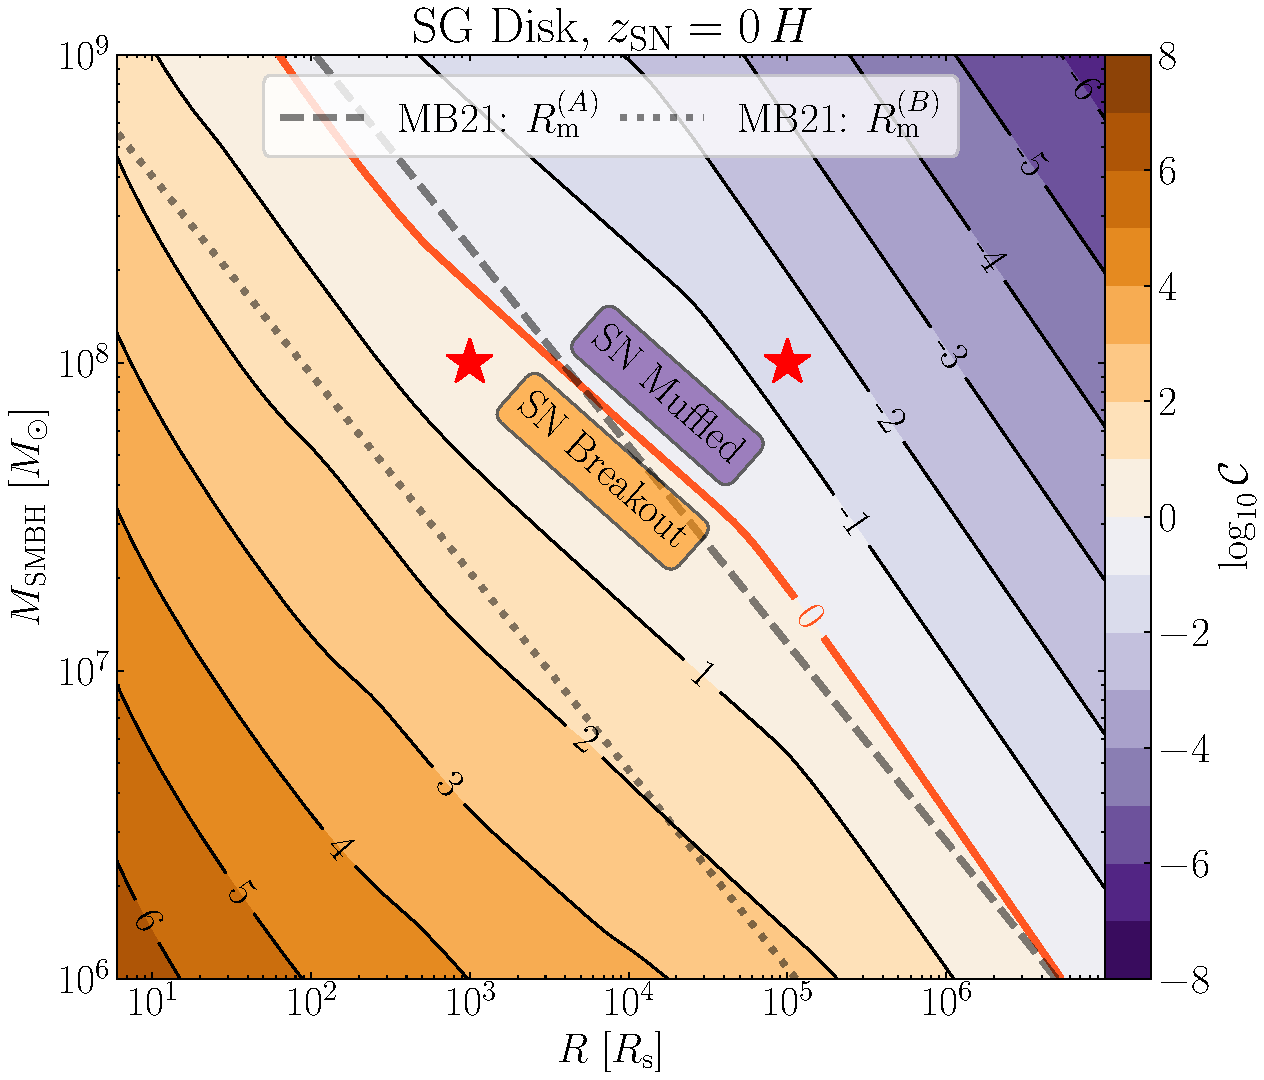
\includegraphics[width=1\linewidth]{ch_snhydro_figs/breakout_sg_midplane.pdf}
    \caption[Breakout parameter $\C$ at height $z=0\,H$ in a SG disk]{Breakout parameter $\C$ versus SMBH mass and radius in an SG accretion disk for SNe detonating at the disk midplane.
    In disks around SMBH with mass $10^6\,\msun$, SNe with energy $10^{51}\,{\rm erg\ s}^{-1}$ will strongly break free from all radii $\leq5\times10^6\,\Rs$.
    The muffling radius decreases in $\Rs$ as SMBH mass increases, reaching $10^2\Rs$ for those with $M=10^9\,\Msun$.
    Stars indicate the $\Mbh$ and radial locations we use to set up our hydrodynamic shearing box simulations to test this prediction.
    The dashed line marks where \citet{Moranchel+21} calculated the muffling radius for SNe when radiative cooling is not important (their scenario A) which closely matches the line for $\C=1$.
    The dotted line marks their scenario B in which radiative cooling becomes important by the free expansion phase, reducing the pressure interior to the shell.}
	\label{fig:breakout-sg}
\end{figure}

\begin{figure}
    \centering
        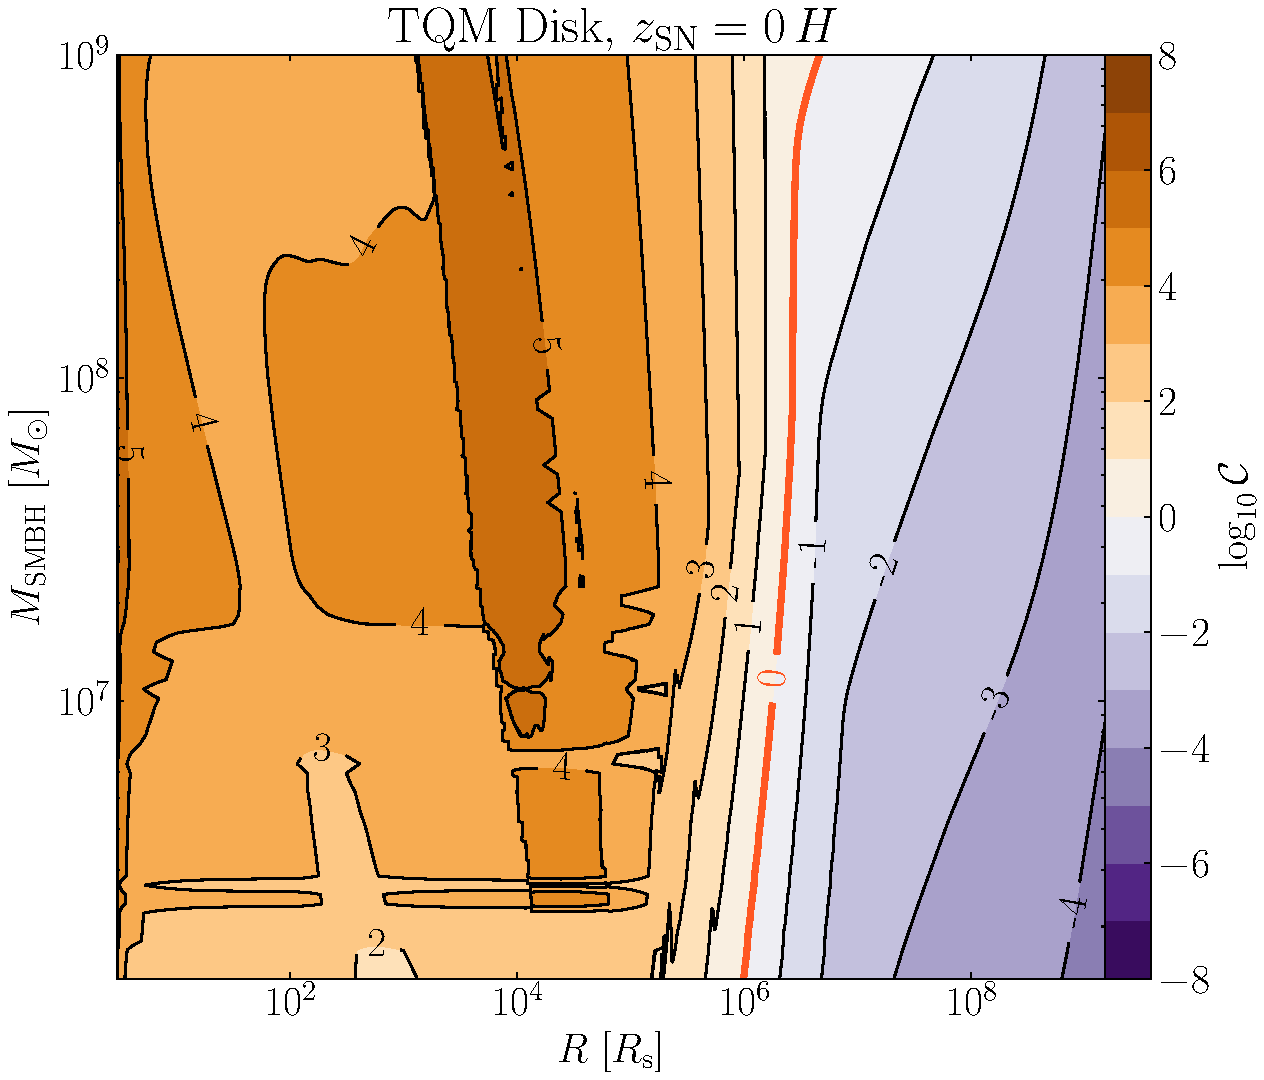
\includegraphics[width=1\linewidth]{ch_snhydro_figs/breakout_tqm_midplane.pdf}
	\caption[Breakout parameter $\C$ at height $z=0\,H$ in a TQM disk]{
	The same as \Fig{fig:breakout-sg} for TQM disks. The location of the muffling radius is located at $\Rm=10^6\,\Rs$ for all SMBH masses.}
    \label{fig:breakout-tqm}
\end{figure}

\begin{figure}
    \centering
    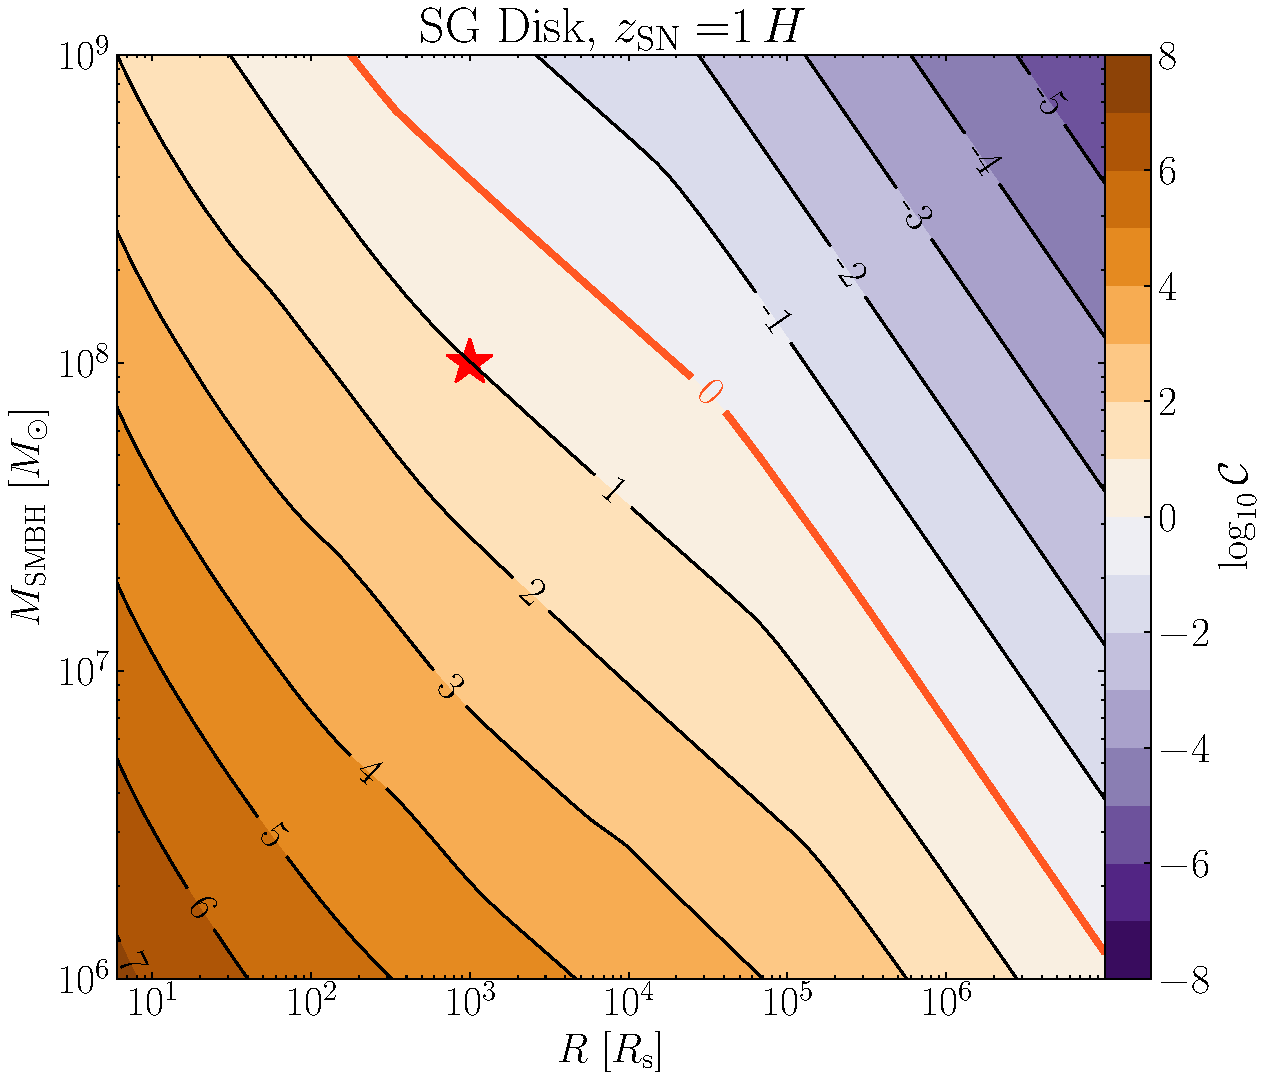
\includegraphics[width=1\linewidth]{ch_snhydro_figs/breakout_sg_z1H.pdf}
    \caption[Breakout parameter $\C$ at height $z=1\,H$]{Breakout parameter $\C$ for SNe at height $z=1\,H$ for an SG disk.
    The lower density offers less resistance to the shock expansion, making breakout easier, and pushing the muffling boundary outward compared to midplane detonations in Fig.~\ref{fig:breakout-sg}.
    The star marks the location that our off-midplane run samples this analytic prediction.}
    \label{fig:breakout-sg-z1h}
\end{figure}


\subsubsection{Hydrodynamics}

We test the muffling radius $\Rm$ marked in red in Fig.~\ref{fig:breakout-sg} for a disk orbiting a $10^8\,\msun$ SMBH by placing our hydrodynamic shearing boxes at $R=[10^3, 10^5]\,\rs$, which have breakout parameters $\C=[2.6, 0.04]$, respectively.
These parameters correspond to the stars in that figure.
The top row of Fig.~\ref{fig:timeseries-composite-xz} shows a time series for a SN at $R=10^3\,\Rs$ and the disk midplane $z_0=0$.
In early times, the shock descends the pressure gradient of the disk and primarily expands vertically until it reaches $z=5\,H$ after 30 days where it is free to expand horizontally along the disk surface.
At this point, the hemispheric expansion evolves symmetrically about the midplane and reaches our domain boundaries at $z=\pm65\,H$ in $\sim80$ days.
The middle row of Fig.~\ref{fig:timeseries-composite-xz} shows the SN placed at $R=10^5\,\rs$ and at the disk midplane.
In contrast to the SN at $10^3\,\rs$, this one remains muffled, only reaching $z\sim1\,H$ over the 1200 years' evolution.
While the SN shock is physically contained at $R=10^5\,\Rs$, the SG disk model is optically thin at this location for $\Mbh \geq 10^7\,\msun$ leaving the possibility that the emitted photons still escape.
The disks' radial ranges in each setup span the same number of scale heights $H$ but the full domains encompass drastically different volumes since $H=10$ AU at $R=10^3\,\Rs$ vs. 16,000 AU $R=10^5\,\Rs$, respectively.
Stellar winds from massive SNe progenitors can carve cavities in the low density gas in the outer disk \citep{Fu-Lin+23}, but the large scale height at $R=10^5\,\Rs$ leaves them unresolved in our models.

The SNe in these two runs occurred directly at the disk midplanes, but in practice the dynamical nature of the AGN system means a star's orbit can be inclined relative to the accretion disk.
The bottom row of Fig.~\ref{fig:timeseries-composite-xz} shows a time series for a setup identical to the top row except we offset the SN initialization vertically to $z_0=1\,H$.
With such a large head start, the upward propagating shock reaches the disk surface in half the time as the midplane case; likewise for the time to reach the boundary.
The plume is slightly more spherical than the midplane case, which directs more of the energy perpendicular to the disk.
The downward shock eventually crosses the midplane and exits the far side of the disk, but the additional material between the SN and midplane slows down the flow which becomes subsonic by the time it reaches the midplane.
We have extended the time series for this run beyond shock-boundary interaction in order to show the flow traveling through the disk.
By allowing the flow to exit the horizontal periodic boundaries, the assumption of a single SN in the disk breaks, but the shock interactions remain at those boundaries and do not affect the source region.

 

\begin{figure*}
    \centering
    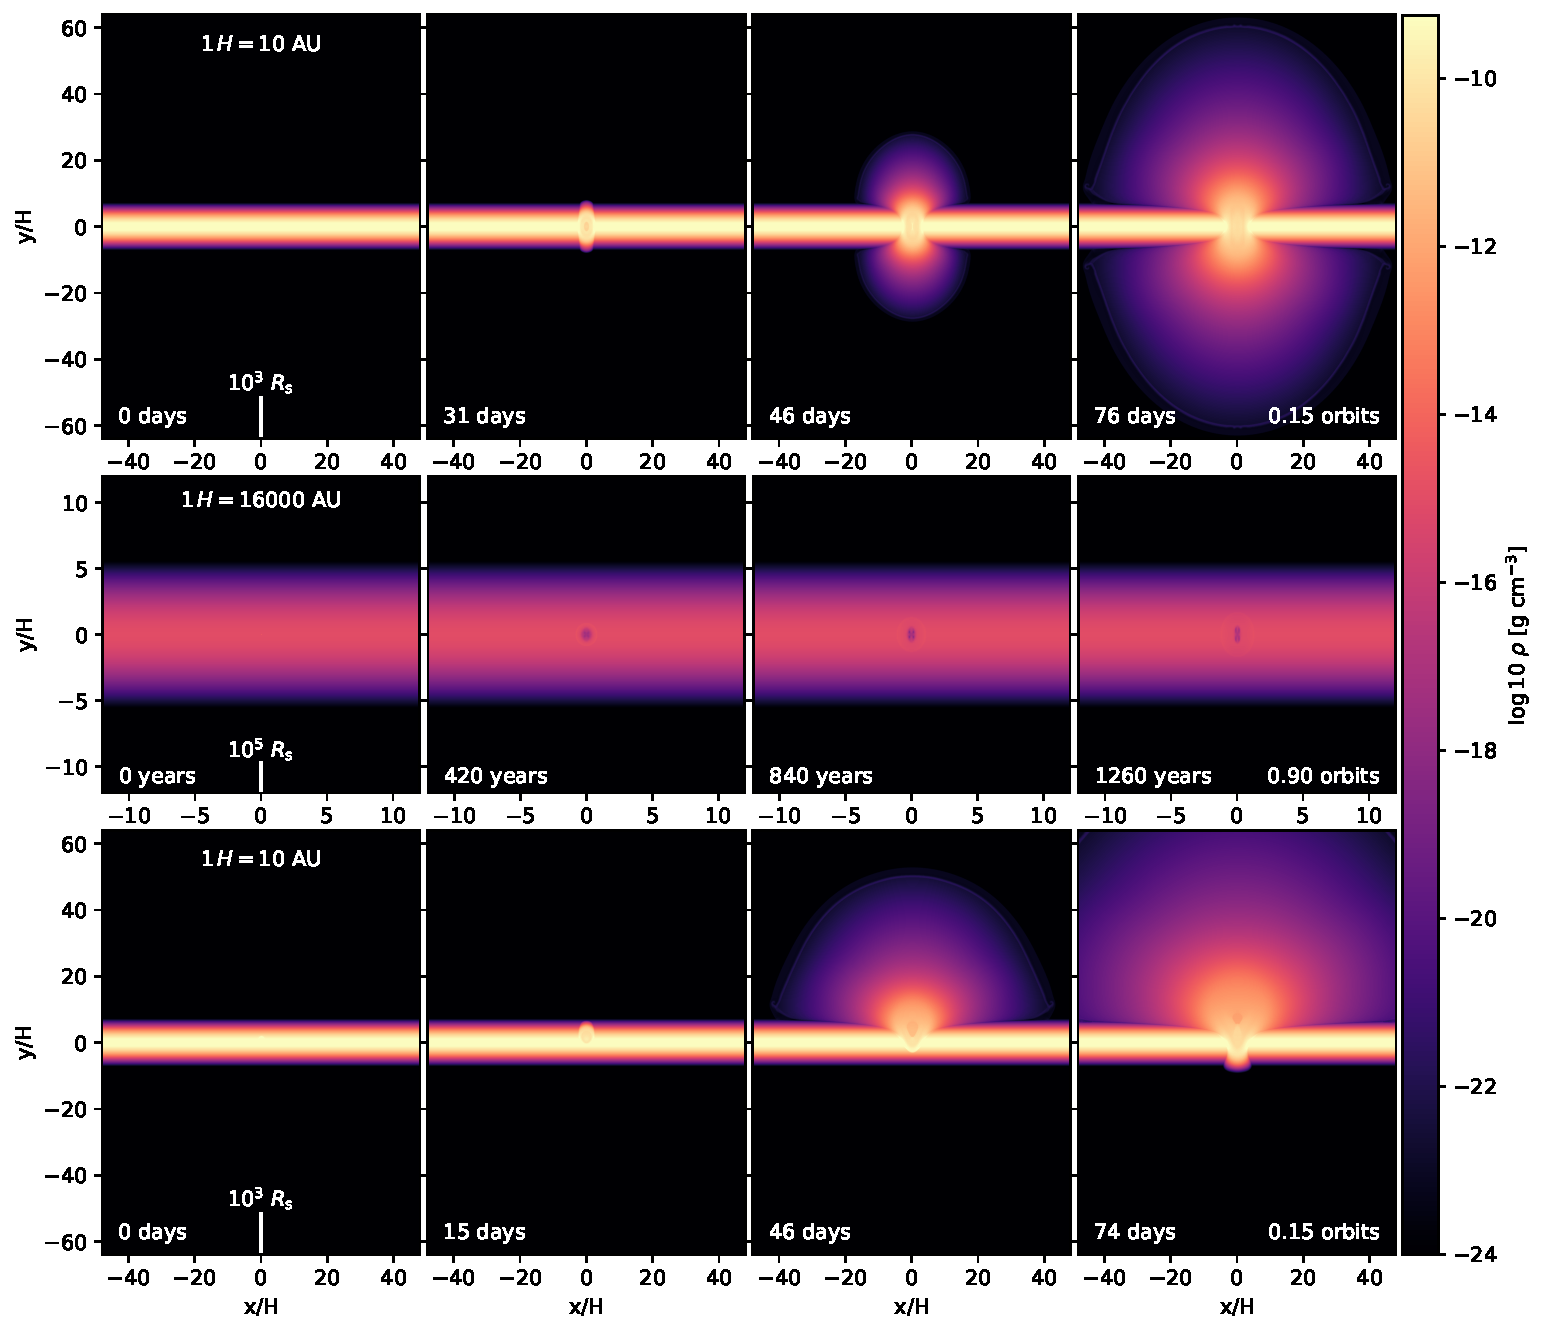
\includegraphics[width=1.0\textwidth]{ch_snhydro_figs/density_xz_timeseries.pdf}
    \caption[$x-z$ gas density time series]{Timeseries of vertical slices ($x-z$) showing the gas volume density evolution for SNe embedded in accretion disks around an SMBH with mass $M=10^8\,\msun$.
    \emph{Top row}: Midplane detonation at $R=10^3\,\Rs$.
    \emph{Middle row}: Midplane detonation at $R=10^5\,\Rs$.
    \emph{Bottom row}: Offset detonation ($z=1H$) at $R=10^3\,\Rs$.}
    \label{fig:timeseries-composite-xz}
\end{figure*}

Fig.~\ref{fig:timeseries-composite-xy} shows the midplane density fields normalized by their respective initial densities.
The main figures in each panel are plotted using the same snapshots and in their native scales (960x960 zones) matching Fig.~\ref{fig:timeseries-composite-xz}, but they have been shifted down and to the left here to accommodate the insets which zoom in on the SNe.
For the midplane run at $R=10^3\,\Rs$ (top row), the shock expands symmetrically until the disk's shear begins to take affect by 0.15 orbits, causing it to elongate slightly along the $y$-direction.
The muffled midplane run at $R=10^5\,\Rs$ (middle row) runs for 0.9 orbits.
Over this longer timescale, the shear effects become more pronounced.
The shock moving leftward towards the SMBH encounters annuli of gas moving at faster orbital velocities which sweep up the shock in a tail wind and pull it forward.
Similarly, the rightward moving shock encounters slower moving gas and conversely lags behind.
Over time, this shearing elongates the cavity made by the SN enough to close it, and shrinks its width almost entirely after 420 years.
The final row shows the SN at $z=1\,H$ reaches the midplane within 15 days, which shears accordingly over the next 60 days.
Recall, the downward flow is subsonic by this point, indicating material that pierces the midplane from an offset SN is not guaranteed to break through as a shock.

\begin{figure*}
    \centering
    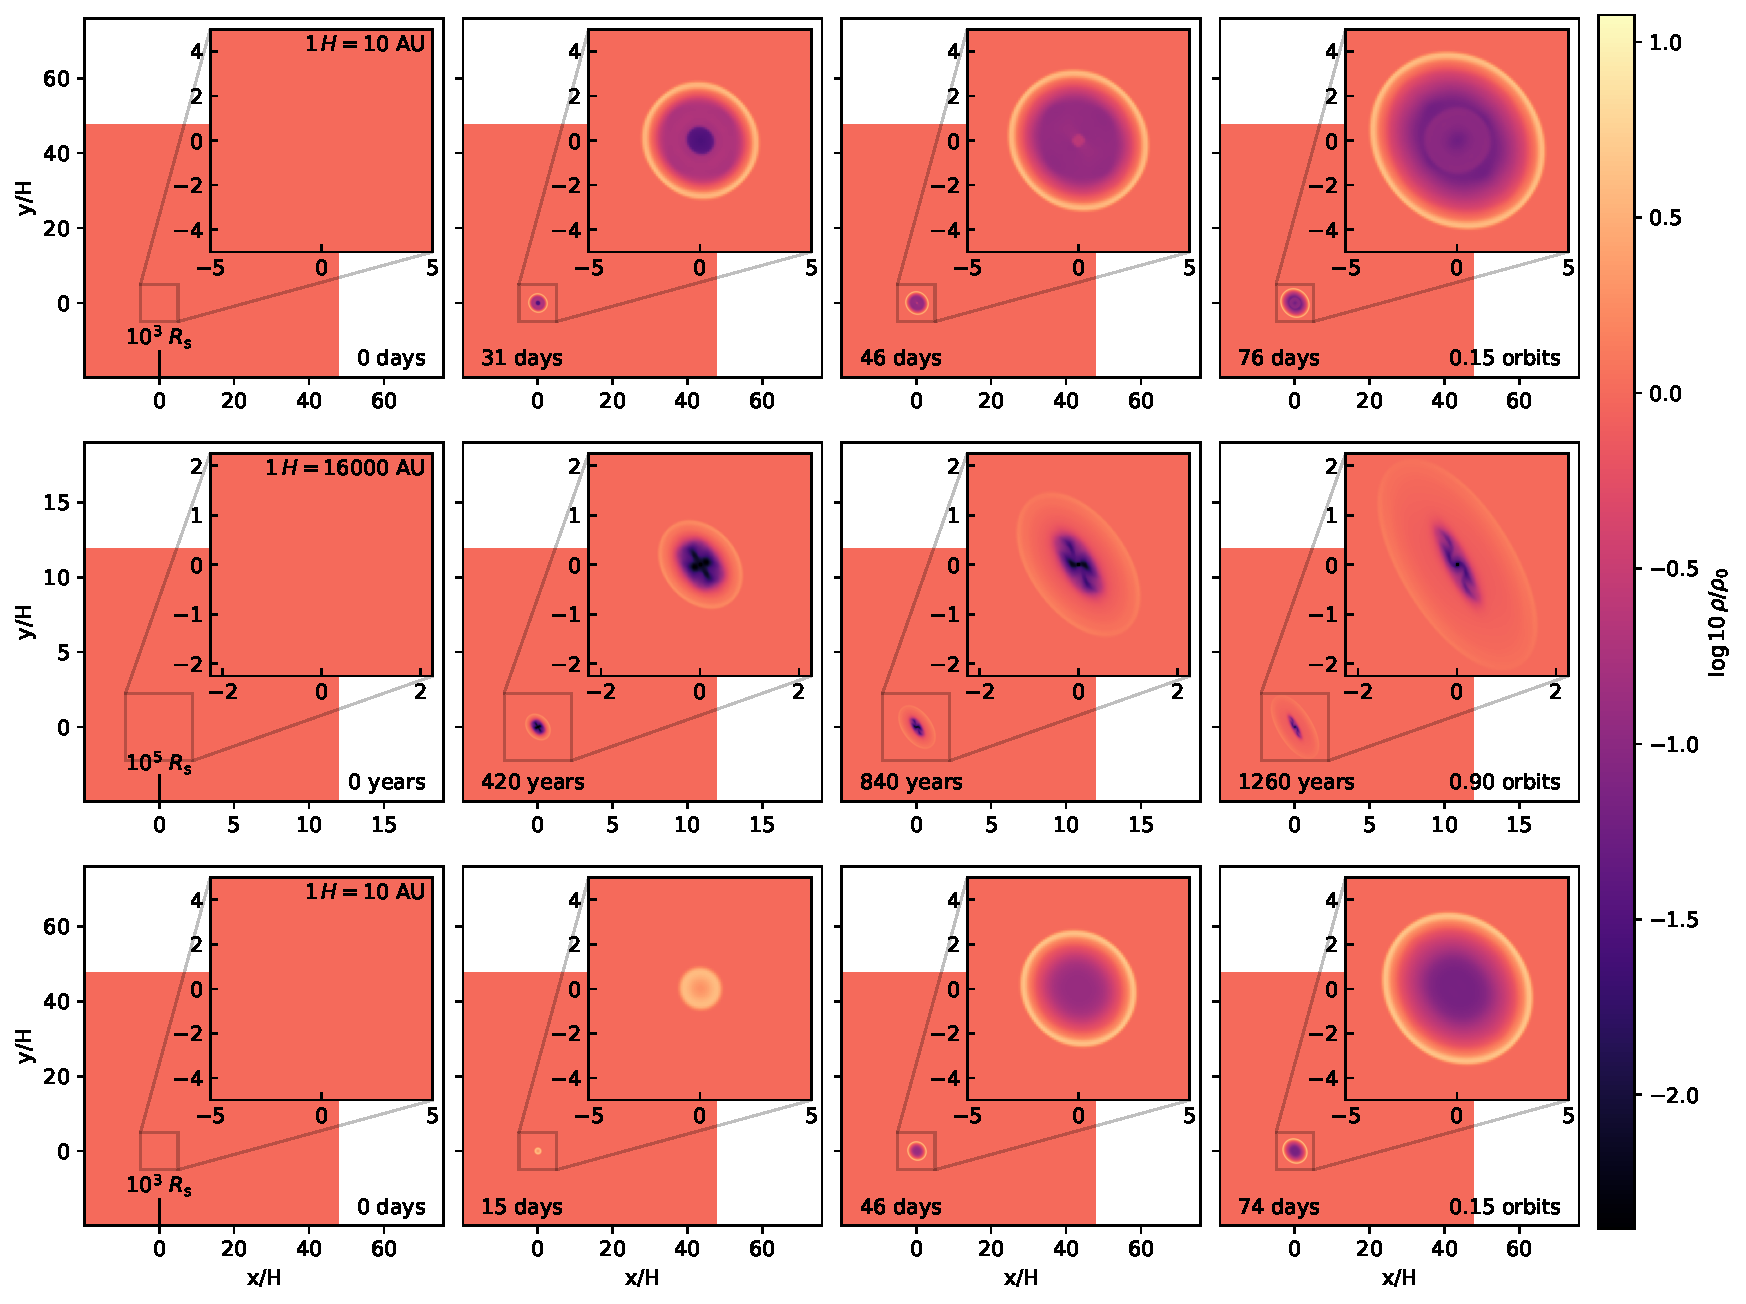
\includegraphics[width=1.0\textwidth]{ch_snhydro_figs/density_xy_timeseries.pdf}
    \caption[$x-y$ gas density time series]{Timeseries of midplane slices ($x-y$) showing the gas volume density evolution for SNe embedded in accretion disks around an SMBH with mass $M=10^8\,\msun$.
    \emph{Top row}: Midplane detonation at $R=10^3\,\Rs$.
    \emph{Middle row}: Midplane detonation at $R=10^5\,\Rs$.
    \emph{Bottom row}: Offset detonation ($z=1H$) at $R=10^3\,\Rs$.}
    \label{fig:timeseries-composite-xy}
\end{figure*}

% ======================
% ======================

\subsection{Discussion} \label{sec:discussion-snhydro}


Whether a SN that occurs at the midplane of an AGN disk breaks free or is muffled depends on its radial location, the mass of the SMBH, and the disk model -- chiefly the local density, temperature, and scale height.

When a SN occurs away from the midplane, the ambient density is lower and the distance the shock must travel in order to break out is smaller than for a midplane detonation at a given radius with the same energy.
This results in shock breakout occurring sooner and retaining more of its initial kinetic energy.
Conversely, the shock propagating towards the far side of the disk must climb the density and pressure gradient of the disk in order to reach the midplane.
In a relatively low density disk, the flow may remain supersonic as it exits the opposite side, but if the disk is dense enough, or the path length to the other side is long enough, the flow may become subsonic well beforehand.
The exact nature of this asymmetrically propagating shock has strong implications for whether radiation reaches two observers located on opposite sides of the disk.
Similar evolution is seen in \citet{Grishin+21}.

As the disk captures stars \citep{MacLeodLin20,Nasim+22} some orbits will begin relatively aligned with it while others will start on highly inclined orbits.
By nature of the geometry, the star will always be embedded at the disk at the nodes where the star's and disk's orbits intersect, and for circular orbits the star will be outside of the disk 90 degrees from the nodes when the inclination is large enough relative to the disk scale height.
Thus, the inclination at which the entire orbit becomes embedded in the disk depends on its semi-major axis and the disk's local scale height, but as the orbit aligns, the star will progressively spend more time embedded within the disk and closer to the midplane.
Our models show that the upward shock from an offset SN on an inclined orbit evolves more rapidly than a midplane SN in the same disk at the same radius.
This holds for midplane a SN in a disk with a midplane density equal to the local density of an inclined SN.

To verify this, we placed a SN at the midplane of a disk with a midplane density equal to the density at $z=1H$ in the offset SN model, i.e., $\rho_0=\rho_{\rm D}(z=1H)\approx5\times10^{-10}$ g cm$^{-3}$ using Eq.\,(\ref{eqn:disk-z-profile}).
The morphology of the plumes that exit the disk are practically identical, but the horizontal expansion into the midplane is slightly larger at corresponding times owing to the lower density.
The vertical shock breakout occurs 6 days ahead of a midplane SN in the denser disk and 10 days behind the inclined SN's. Having been slowed down as it climbed out from the midplane, the flow traveling along the disk surface has a slower velocity, reaching the boundary 13 days behind the inclined SN.

Lateral shock expansion into the midplane is small, $\Delta r\approx 10\,H$ at $10^3\,\Rs$.
The relative size of this cavity to its location is $\Delta r/R = 0.05$.
The evolution time is short relative to the orbital period, so the midplane cavities remain close to circular.
Over long times, on the order of the orbital period, the horizontal shock will stall as the shear elongates the cavity until it closes.
Thus, a single SN will have minimal impact on the disk structure and the cavity will close as it stalls and the shear deforms it.

If AGN disks with structures described by the SG model are common, then for a fiducial $\Mbh=10^8\,\Msun$, any observed AGN-SN would have occurred within $10^3\,\Rs$ ($<$1000 AU), corresponding to $\sim5$ light days.
This is inside the broadline region that is a few light weeks to typically a light month in size depending on $\Mbh$ \citep{BlandfordMcKee82}.
This means that the response of the broadlines to the new SN illumination would be roughly symmetric.
Conversely, if the SN happens at large radii in a lower density disk, then the response will be infrared-bright.
Thus, the observational details allow us to use SN to infer its location and probe the disk's properties.

If the SN occurs in the inner disk, the orbital time can be short.
The top row of Fig.~\ref{fig:timeseries-composite-xz} occurs in about 15\% of the orbital period ($\sim3$ years $\sim1000$ days) at $R=10^3\,\Rs$ for $\Mbh=10^8\,\Msun$.
SNe occurring here should lead to redshifted or blueshifted asymmetries in the lines due to the Doppler effect since the orbital speed is of the order $10^4$ km s$^{-1}$.
Similar asymmetries have been observed in AGN broadline profiles that are possibly caused by localized inconsistencies in the disk structure \citep[e.g., spiral arms,][]{Schimoia+17}.
An inner-disk SN may be ruled out as the catalyst for an AGN flare if the spectrum does not exhibit these features.

AGN disks are observed to have elevated metallicities across redshift \citep{Dors+14,Onoue+2020}.
Muffled SNe may be a contributing source by infusing the disk with localized pockets of metals.
SNe in the breakout region will similarly enhance the midplane metallicity, but the plume that emerges from the disk will neither expand into the steady-state, uniform medium as we have modeled nor retain the quasi-hemispheric shape we see in Fig.~\ref{fig:timeseries-composite-xz}.
Rather, it will encounter an intense radiation field emitted by the hot corona of the BH that drives outflows along the disk surface, blowing the plume to larger radii \citep{CrenshawKraemerGeorge03,ProgaKallman04}.
As the wind drives the SN ejecta at speeds of $10^2-10^5$ km s$^{-1}$ \citep{Parker+17,Mehdipour+17}, it will spiral outward, scattering nucleosynthetically enriched material across the outer disk.
If SNe are a significant contributor to AGN metal fractions, that likely indicates a top-heavy stellar mass function \citep{FanWu23} and that embedded stars evolve off the main sequence during the AGN's active phase \citep{HuangLinShields23} as opposed to doing so after the disk fully accretes \citep{CantielloJermynLin21}.

The SG disk model may only represent one phase of the accretion process over the course of an AGN lifetime.
Disks in lower states of accretion will be more tenuous like the TQM model, allowing the SN to expand further into the midplane, excavate a larger portion of the disk atmosphere, and cause more disruption.
Neither of these models consider magnetic fields that are carried into the disk by parcels of gas as they accrete from the torus.
As magnetic fields build, the additional pressure becomes an important component of the overall disk pressure.
Even fields that produce a plasma $\beta \equiv P_{\rm gas} / P_{\rm mag} = 10^{2.5}$ in the midplane can become magnetically dominated away from the midplane and effectively increase the scale height relative to disks with much weaker fields at $\beta=10^4$ \citep{Gerling-Dunsmore+25}.
Since $H$ is the primary characteristic of an AGN disk for determining shock breakout, the magnetic fields could move the muffling radius inwards if the gas density remains similar to cases with no magnetic fields.
In extreme cases, disk models following gas flows in cosmological simulations down to within a few Schwarzschild radii demonstrate buildup of strong magnetic fields reaching $\beta \sim 10^{-6} - 10^{-2} \ll 1$ \citep{Hopkins+25}.
These flux-frozen disks suppress star formation entirely, implying the progenitors of any AGN-SNe must be captured by the disk from the nuclear star cluster \citep{Fabj+20,Nasim+22}.

In the case where star formation can occur in the disk, the AGN-SN rate is estimated to be $\dot{N}_{\rm SN}\sim10^{-2}\,{\rm yr}^{-1}$ for $\Mbh=10^8\,\Msun$ \citep{HuangLinShields23}.
If the density of AGN in the Universe is $n_{\rm AGN}=10^6$ Gpc$^{-3}$ \citep{OsterbrockFerland06}, the rate density of AGN-SNe is $\mathcal{R_{\rm SN}} \sim 10^4$ yr$^{-1}$ Gpc$^{-3}$.
Phenomena related to AGN activity may be visible for a range timescales spanning $10^4$ yr \citep{Morganti17} to $10^6$--$10^8$ yr \citep{Biava+21} depending on the specific mechanism being probed, but some modeling suggests the dense disks we consider here have a lifetime on the order of $\tau_{\rm AGN}=10^6$ yr \citep{Angles-Alcazar+21}.
Given $\dot{N}_{\rm SN}$ over that lifetime, the number of SNe that occur within the disk for a typical AGN is $\mathcal{N}_{\rm SN}=10^4$ AGN$^{-1}$.

However, not all SNe will break free from the disk as we have shown.
If we assume SNe occur evenly throughout a disk with outer radius of $10^7\,\Rs$ and a muffling radius at $\Rm\sim10^4\,\Rs$, then we need to scale by the fraction of the disk area that allows breakout $f_{\rm b} = (\Rm / R_{\rm disk})^{2} = 10^{-6}$.
Thus, the breakout rate per AGN becomes
\begin{equation}
    \mathcal{N_{\rm b,SN}} \sim 10^{-2} \left( \frac{f_{\rm b}}{10^{-6}} \right) \left( \frac{\dot{N}_{\rm SN}}{\rm 10^{-2}\ \frac{SN}{yr\ AGN}} \right) \left( \frac{\tau_{\rm AGN}}{\rm 10^6\ yr} \right) \mathrm{AGN^{-1}},
\end{equation}
and the volume rate similarly reduces to
\begin{equation}
    \mathcal{R_{\rm b,SN}} \sim 10^{-2} \left( \frac{f_{\rm b}}{10^{-6}} \right) \left( \frac{\dot{N}_{\rm SN}}{\rm 10^{-2}\ \frac{SN}{yr\ AGN}} \right) \left( \frac{n_{\rm AGN}}{\rm 10^6\ \frac{AGN}{Gpc^3}} \right) \mathrm{Gpc^{-3}\ yr^{-1}}
\end{equation}

This chapter explored the possibility of SN shocks breaking free from the disk.
\citet{Moranchel+21} and \citet{Grishin+21} approached this question with different methods yet achieved similar results for midplane and off-set scenarios.
Whether radiation emitted by a SNe can be observed against the bright AGN disk is a separate matter and depends on the optical depth through the disk to the detonation site.
For example, even though the shock in the model placed at $R=10^5\,\Rs$ was muffled, the SG disk model is optically thin at that radius when $\Mbh=10^8\,\Msun$, and photons directly emitted by a SN may still escape.
We will present detailed post-processing radiative transfer calculations to derive light curves for our shearing box simulations in the following chapter.

As large surveys like the LSST generate baselines for substantially more AGN \citep{Kovacevic+22}, if we are able to constrain the rates of observable and non-observable AGN-SN, we will also have constraints on AGN disk properties such as their sizes and densities.
If the rate is small, then either most SNe are muffled in a geometrically thick, low-density AGN disk or the disk is typically small.
In contrast, a large rate suggests AGN disks are likely large, geometrically thin, dense, and thus able to capture or produce stars at a high rate.

Though we have considered Type II SNe ejecting $10\,\msun$ envelopes, AGN-embedded stars may not evolve like stars in the field, changing our rate estimates and details of the explosions such as the ejecta mass and energy of the SN \citep{CantielloJermynLin21, DittmannJermynCantiello23}.
Similarly, Type Ia supernovae from accreting white dwarfs and kilonovae from binary neutron stars formed by the disk, also possible sources of AGN transients, likely evolve differently when embedded in an AGN disk.

% ======================
% ======================

\subsection{Conclusions}
\label{sec:conclusions-snhydro}
Massive stars in nuclear star clusters on orbits embedded in AGN accretion disks may detonate as SNe from within the disk.
The shock can break free from the disk if its internal pressure exceeds the ambient disk pressure and is muffled otherwise.
The exact outcome depends on the radial and vertical location of the detonation as described by Eq.\,(\ref{eqn:C-parameterized}).
We performed hydrodynamic three-dimensional shearing box simulations at two locations on either side of the muffling boundary of embedded SNe and found agreement with the analytic prediction for shock breakout from an SG-type AGN disk orbiting a black hole of mass $\Mbh=10^8\,\Msun$.
Specifically, we found:

\begin{itemize}
    \item In general, SNe break free from the inner disk, whereas the outskirts of AGN disks muffle them,
    \item In SG disks, when $\mbh=10^6\,\msun$, the muffling boundary occurs at $R_{\rm m}=5\times10^6\,\rs$ ($\sim10^6$ AU) and moves inward to $R_{\rm m}=100\,\Rs$ ($\sim100$ AU) in disks around $\mbh=10^9\,\msun$,
    \item In TQM disks, the muffling radius lies at $R_{\rm m}=10^6\,\Rs$, regardless of the SMBH's mass,
    \item The muffling radius for SNe that occur at $z>1\,H$ shifts outwards by approximately one order of magnitude in comparison with midplane detonations,
    \item When SNe detonate away from the midplane the ejecta traveling to the far side of the disk may remain shocked or emerge as subsonic flows depending on the gas density and scale height, where the optical thickness will determine whether photons do the same,
    % Shocks from SNe detonating away from the midplane at heights $z>1\,H$ may not break through to the other side of the disk \textbf{or may do so as a subsonic }, 
    \item When the SN occurs away from the midplane, the shock propagating away from the disk expands rapidly in comparison to the shock propagating towards (and possibly through) the midplane, slowing down as it climbs the density and pressure gradients,
    \item Considering a lifetime of $\tau_{\rm AGN}=1$ Myr and a SN rate in the disk of $\dot{N}_{\rm SN} \sim 10^{-2}$, we estimate a rate of $\mathcal{R}_{\rm b} \sim 10$ SN AGN$^{-1}$ yr$^{-1}$ breaking free from the disk and estimate a volumetric rate density of $\mathcal{R}_{\rm SN} \sim 10$ Gpc$^{-3}$ yr$^{-1}$ for the local Universe.
\end{itemize}


As Vera Rubin Observatory and LSST expand our transient catalogs, automated search algorithms may identify light curves with previously unobserved characteristics or features.
One potential source of these new transients could be AGN-embedded SNe whose light curves are altered by an AGN disk.
In the following chapter we will describe results from our radiative transfer analysis of the models presented here.
Combining radiative and kinematic SNe muffling may reveal information about an average disk's structure, leading to a broader understanding of AGN accretion physics and galactic nuclei in general.






% \end{document}


\clearpage
\resetcounters
\addtocontents{toc}{\protect}
\section{\texorpdfstring{\MakeUppercase{radiative transfer models and observables of supernovae in active galactic nuclear accretion disks}}{radiative transfer models and observables of supernovae in active galactic nuclear accretion disks}}
\label{sec:sn-rt}

\counterwithin{figure}{section}
\counterwithin{table}{section}


Here we describe the radiative transfer models we apply as post-processing to the three-dimensional hydrodynamic models described in the previous chapter.
The content will be submitted to the \textit{Astrophysical Journal} for publication.
Please cite Cook et al. (2026b) when possible.


\subsection{Methods} \label{sec:methods}

% ======================
% ======================

\subsubsection{Vertical Temperature Profile} \label{subsec:temperature-profile}

The disk models in Ch.~\ref{sec:sn-hydrodynamics} were initialized isothermally by setting the sound speed according to the midplane temperature $\Tmid$ at the SN's radius in a \citet{SirkoGoodman03} disk.
In hydrostatic equilibrium an isothermal disk has a vertical density profile that is Gaussian, which is a good approximation for the temperature in passive disks (those heated by an external source).
Active disks (those internally heated) are much hotter in the midplane and have much more complicated vertical structures, and determining the $T(z)$ dependence is non-trivial.
For this study, we apply a temperature mask over the entire domain for each snapshot of the form
\begin{equation}
\label{eqn:temp-profile}
    T(z) =
    \begin{cases}
	\Tiso & T>\Tmid \\
	\Tmid e^{- \frac{z^2}{2 H_T^2}} & \Tfloor < T < \Tmid \\
	\Tfloor & T<\Tfloor
    \end{cases}
\end{equation}
where $\Tfloor=2000$ K.
We could use simply $\Tiso = \Tmid$, but in practice we find that we need to allow for some flexibility in regions modified by the SN Gaussian in the initial conditions.
As such, we set $\Tiso = (1+\epsilon) \Tmid$, and find empirically that $\epsilon=10^{-2}$ gives acceptable results.
We find the temperature scale height $H_T=1.7\,H$ by root-solving for the profile from the midplane temperature to the effective temperature $\Teff$ using the Eddington approximation
\begin{equation}
	T = \left( \frac{3}{8} \tau + \frac{1}{2} + \frac{1}{4\tau} \right)^{1/4}\ \Teff.
\end{equation}
where we calculate $\tau$ using the Rosseland mean opacity given the vertical disk density profile.
This formulation allows us to bypass regions modified by the SN and only apply the disk profile to zones where the disk is unchanged.


% ======================
% ======================

%
%  Section on Light Curves
%
\subsubsection{Radiative Transfer Post-Processing} \label{subsec:rad-transfer}


We calculate the wavelength-dependent continuum intensity emerging from the hydrodynamic models via post-processing including attenuation from absorption and scattering processes along each column.
The cooling timescale is long compared to the dynamical timescale for our setup, so we can consider the gas to be adiabatic since radiative losses are small.
We solve the following form of the radiative transfer equation,
\begin{equation}\label{eqn:RadTrans}
    \cos\theta \frac{1}{(\kappa_\lambda + \sigma_\lambda)\rho} \frac{dI_\lambda}{dz} = -I_\lambda + S_\lambda,
\end{equation}
where $\theta$ is the direction of propagation, $\kappa_\lambda$ is the opacity due to true absorption, $\sigma_\lambda$ is the scattering opacity, $\rho$ is the volumetric gas density, $I_\lambda$ is the radiation field's intensity, and $S_\lambda$ is the source function.
The presence of scattering calls for an effective source function that depends on the Planck function $B_\lambda$ and the mean intensity $J_\lambda$,
\begin{align}
    S_\lambda &= \frac{\kappa_\lambda B_\lambda + \sigma_\lambda J_\lambda}{\kappa_\lambda + \sigma_\lambda}  \nonumber\\
              &= (1-\omega_\lambda) B_{\lambda} + \omega_\lambda J_\lambda \label{eqn:effective_source}
\end{align}
where $\omega_\lambda = \sigma_\lambda / (\kappa_\lambda + \sigma_\lambda)$ is the single-scattering albedo.
The subscript $\lambda$ indicates quantities with wavelength dependence.
By restricting $\theta$ to be either 0 or $\pi$, we adopt the two-stream approximation which allows the radiation field to travel only upwards ($\Iplus$) or downwards ($\Iminus$), respectively, along the $z$-axis through independent columns of cells located at a given $(x, y)$ position.
First, we tried direct integration like in \citet{Godines+26}, but unlike a protoplanetary disk, an AGN disk is not isothermal and does not allow for this crude integration which lost too much flux in the non-conservative direct integration due to exponentially changing intensities.
Therefore, each column is treated as an isolated stream and is solved using the Feautrier method \citep{Feautrier64,Cannon70}, an implicit method which calculates the mean intensity at each point simultaneously.
%See Appendix \ref{sec:Apdx-Feautrier} for our modification of the method to include scattering and our boundary conditions.
It is appropriate for the general case where extinction occurs via absorption and scattering processes.

This method outlined below forms the core of the \ocotillo code, a multi-wavelength post-processing radiative transfer calculation that we developed for this purpose.

\subsubsubsection{Feautrier method}
\label{sec:Feautrier-method}

To begin, we adopt the two stream Eddington approximation for the radiation field by taking $\theta = 0$ (along z) and $\pi$ (opposite to z) in \eq{eqn:RadTrans}.
This leads to a set of two equations for each stream: $\Iplus_\lambda$ upwards and $\Iminus_\lambda$ downwards, respectively.
With $\alpha_\lambda = \rho(\kappa_\lambda + \sigma_\lambda)$,
\begin{align} 
    \frac{1}{\alpha_\lambda}\frac{d\Iplus_\lambda}{dz} &= -\Iplus_\lambda + S_\lambda \label{eqn:dIpdz}, \\
    -\frac{1}{\alpha_\lambda}\frac{d\Iminus_\lambda}{dz} &= -\Iminus_\lambda + S_\lambda. \label{eqn:dImdz}
\end{align}
The effective source function $S_\lambda$ defined in \eq{eqn:effective_source} is composed of the Planck function
\begin{equation}
    B_{\lambda}(T) = \frac{2hc^2/\lambda^5}{\exp(hc/\lambda k T) - 1},
\end{equation}
and the mean intensity
\begin{equation}
    J_\lambda = \frac{1}{4\pi}\int I_\lambda d\Omega.
\end{equation}
We now drop the subscript $\lambda$ for clarity.
Adding \eq{eqn:dIpdz} to \eq{eqn:dImdz}
\begin{equation}\label{eqn:dIdz}
    \frac{1}{\alpha}\frac{d(\Iplus + \Iminus)}{dz} = - (\Iplus - \Iminus).
\end{equation}
Dividing by two and defining the mean intensity as 
\begin{equation}
    U = \frac{\Iplus + \Iminus}{2}
\end{equation}
and the flux as
\begin{equation}
    V = \frac{\Iplus - \Iminus}{2},
\end{equation}
\eq{eqn:dIdz} simplifies to
\begin{equation}\label{eqn:dUdz=-V}
    \frac{1}{\alpha}\frac{dU}{dz} = -V.
\end{equation}
Subtracting \eq{eqn:dImdz} from \eq{eqn:dIpdz}
\begin{equation}
    \frac{1}{\alpha}\frac{d(\Iplus - \Iminus)}{dz} = - (\Iplus + \Iminus) + 2S.
\end{equation}
Again, dividing by two with the same substitutions and remembering the effective source function \eqp{eqn:effective_source},
\begin{equation}
    \frac{1}{\alpha}\frac{dV}{dz} = -U + (1-\omega) B + \omega J.
\end{equation}
In the two-stream approximation $J=U$ simplifying the previous equation further to
\begin{equation}
    \frac{1}{\alpha}\frac{dV}{dz} = -(1-\omega) U + (1-\omega) B. \\
\end{equation}

Now, we have two equations for the mean intensity $U$ and flux $V$
\begin{align}
    \frac{1}{\alpha}\frac{dU}{dz} =& -V; \label{eqn:dUdz} \\
    \frac{1}{\alpha}\frac{dV}{dz} =& (1-\omega)(B-U). \label{eqn:dVdz}
\end{align}
Substituting $V$ into the second leaves one equation in $U$,
\begin{equation}\label{eqn:ddU/ddz}
    \frac{d}{dz} \left( \frac{1}{\alpha} \frac{dU}{dz} \right) = -\alpha(1-\omega)(B-U).
\end{equation}

Next, we discretize $U$ onto a uniform grid (i.e., $\Delta z =$ const).
To evaluate the point $i$ using centered derivatives, we define the fluxes $\phi$ at the half-grid points
\begin{equation}\label{eqn:U_i-discrete}
    \frac{\Delta}{\Delta z} \left( \frac{1}{\alpha_i}\frac{\Delta U_i}{\Delta z} \right) = \frac{\phi_{i+\sfrac{1}{2}} - \phi_{i-\sfrac{1}{2}}}{\Delta z}
\end{equation}
where the fluxes at the cell interfaces $i\pm\sfrac{1}{2}$ are calculated using the forward and backward points
\begin{eqnarray}
    \phi_{i+\sfrac{1}{2}} = \frac{1}{\alpha_{i+\sfrac{1}{2}}} \frac{(\Uipone - \Ui)}{\Delta z}, \\
    \phi_{i-\sfrac{1}{2}} = \frac{1}{\alpha_{i-\sfrac{1}{2}}} \frac{(\Ui - \Uimone)}{\Delta z}.
\end{eqnarray}

Using \eq{eqn:U_i-discrete} to replace the left-hand side of \eq{eqn:ddU/ddz}
\begin{equation}
      \frac{1}{\alpha_{i+\sfrac{1}{2}}} \frac{(\Uipone - \Ui)}{\Delta z} 
    - \frac{1}{\alpha_{i-\sfrac{1}{2}}} \frac{(\Ui - \Uimone)}{\Delta z}  
    = - \alpha_i (1 - \omega_i)(B_i - \Ui) \Delta z
\end{equation}
and collecting terms in $U$
\begin{equation}
    \frac{1}{\alpha_{i+\sfrac{1}{2}}} \Uipone - \left[ \frac{1}{\alpha_{i+\sfrac{1}{2}}}+ \frac{1}{\alpha_{i-\sfrac{1}{2}}} + \xi_i  \right] \Ui + \frac{1}{\alpha_{i-\sfrac{1}{2}}} \Uimone  = - \xi_i B_i,
\end{equation}
where $\xi_i = \alpha_i (1 - \omega_i) \Delta z^2$, we arrive at a form that can be constructed as a system of equations for each $i$ in matrix form with $\Ui$ along the diagonal and the $\Uimone$ and $\Uipone$ terms falling along the left and right off-diagonals, respectively, 
\begin{equation}
    a_i \Uipone + b_i \Ui + c_i \Uimone = d_i, \label{eqn:system-in-U_i}
\end{equation}
where
\begin{eqnarray}
    a_i &=& 1/\alpha_{i+\sfrac{1}{2}} \\
    c_i &=& 1/\alpha_{i-\sfrac{1}{2}} \\
    b_i &=& -a_i - c_i - \xi_i \\
    d_i &=& - \xi_i B_i
\end{eqnarray}
This tridiagonal matrix can be solved using standard methods for the mean intensity at each point.
Then, using \eq{eqn:dUdz=-V} we can solve for the flux $V$ and upwards $\Iplus$ and downwards $\Iminus$ intensities using the definitions for $U = \Iplus + \Iminus$ and $V = \Iplus - \Iminus$.

The quantities at the domain boundaries represent the observable radiation field.
The flux defined in the two-stream approximation is converted into the flux density by $F_\lambda = 2 \pi V_\lambda$.

\subsubsection{Boundary Conditions}
We set the radiation field at the vertical boundaries to be outflow only.
Considering $U = (\Iplus + \Iminus) / 2$ and $V = (\Iplus + \Iminus) / 2$, outflow boundaries imply the lower boundary at $z=-L/2$ has an upward intensity $\Iplus=0$, such that $U(z=0) = \Iminus/2$ and $V(z=0)=-\Iminus/2$, and thus $U=-V$.

In order to match the second order in $\Delta z$ we expand $U$ close to the boundary in a Taylor series
\begin{equation}
    U_{\sfrac{1}{2}} = U_0 + \frac{\Delta \tau}{2} \left. \frac{dU}{d\tau} \right|_0 + \frac{\Delta \tau^2}{8} \left. \frac{d^2U}{d\tau^2}\right|_0
\end{equation}
Substituting $U_{\sfrac{1}{2}} = (U_0 + U_1)/2$,
\begin{equation}
    \frac{U_1 + U_2}{2} = U_0 + \frac{\Delta \tau}{2} \left. \frac{dU}{d\tau} \right|_0 + \frac{\Delta \tau^2}{8} \left. \frac{d^2U}{d\tau^2}\right|_0.
\end{equation}
Using \eq{eqn:dUdz} -- \eq{eqn:ddU/ddz}, we have the first and second derivatives of $U$ in $\tau$.
Evaluating these at $z=0$
\begin{align}
    \left. \frac{dU}{d\tau} \right|_0 &= U_0 \text{  (since}\ U_0=-V_0 \text{ for } \Iplus=0), \\
    \left. \frac{d^2U}{d\tau^2}\right|_0 &= (1-\omega_0)(U_0-B_0),
\end{align}
and the expression for $U_{\sfrac{1}{2}}$ becomes
\begin{equation}
    \frac{U_0 + U_1}{2} = U_0 + \frac{\Delta \tau}{2} U_0 + \frac{\Delta \tau^2}{8} (1-\omega_0)(U_0-B_0).
\end{equation}
Collecting terms in $U_i$
\begin{equation}
    U_0 \left[ -1-\Delta \tau - \frac{\Delta \tau^2}{4}(1-\omega_0) \right] + U_1 = - \frac{\Delta \tau^2}{4}(1-\omega_0)B_0.
\end{equation}
Reintroducing $\Delta \tau =\alpha \Delta z$,
\begin{equation}
    U_0 \left[ -1-\alpha_0\Delta z - \frac{\alpha_0^2\Delta z^2}{4}(1-\omega_0) \right] + U_1 = - \frac{\alpha_0^2\Delta z^2}{4}(1-\omega_0)B_0.
\end{equation}
Dividing by $\alpha_0$, the coefficients as defined in \eq{eqn:system-in-U_i} have the quantities
\begin{eqnarray}
    a_0 &=& 0, \\
    b_0 &=& -1\left[ \frac{1}{\alpha_0} + \Delta z + \frac{\alpha_0 \Delta z^2}{4}(1-\omega_0) \right], \\
    c_0 &=& 1/\alpha_{0}, \\
    d_0 &=& - \frac{\alpha_0 \Delta z^2}{4}(1-\omega_0) B_0.
\end{eqnarray}
At the upper boundary $z=L/2$, the downward intensity $\Iminus=0$ leading to $U_N=V_N$.
The same exercise as above results in the coefficients
\begin{eqnarray}
    a_N &=& 1/\alpha_N, \\
    b_N &=& -1\left[ \frac{1}{\alpha_N} + \Delta z + \frac{\alpha_N \Delta z^2}{4}(1-\omega_N) \right], \\
    c_N &=& 0, \\
    d_N &=& - \frac{\alpha_N \Delta z^2}{4}(1-\omega_N) B_N.
\end{eqnarray}
We call attention here to an important subtlety, that the Taylor expansion near the boundary gives the coefficients the same order in $\alpha$ and $\Delta z$ as those for the rest of the domain.

\subsubsection{Opacities}
Given the density and temperature of a zone, we solve for the populations of neutral hydrogen H, ionized hydrogen $\Hplus$, the negative hydrogen ion $\Hminus$, and free electrons.
The neutral and negative ion species absorb radiation when an electron is stripped away through the bound-free (bf) ionization process, $\kappa(\text{H}_\text{bf})$ and $\kappa({\Hminus_\text{bf}})$ respectively, and the positive and negative hydrogen ions absorb photons via free-free (ff), or Bremsstrahlung, interactions with free electrons, noted as $\kappa (\text{H}_\text{ff})$ and $\kappa (\Hminus_\text{ff})$.
%We calculate the combined continuous absorption from these processes, following \citet{Gray76,Gray21}, as
%\begin{align}
%       \kappa_\lambda =& \biggl\{ \bigl[ \kappa(\text{H}_\text{bf}) + \kappa(\text{H}_\text{ff}) + \kappa(\text{H}^-_\text{bf}) \bigr] (1 - 10^{-\chi \theta}) \nonumber \\
%		    &+ \kappa(\text{H}^-_\text{ff}) \biggr\} \frac{1}{1 + \Phi_\text{H}(T) / P_\text{e}}  + \kappa(\text{e}^-).
%\end{align}
%The factor $1-10^{-\chi\theta}$ accounts for the stimulated emission of H and $\Hminus$ with $\theta = 5040 / T\ \text{eV}^{-1}$ and $\chi(\lambda) = 1.2398 \times 10^4 / \lambda\ \text{eV}$ when $T$ is in Kelvin and $\lambda$ is in \r{a}ngstr\"om.
%The ionization state $\Phi_\text{H}(T)$ is given by the Saha equation, and $P_\text{e}$ is the partial pressure due to free electrons.
%Though scattering processes in general can be wavelength-dependent, the scattering coefficient for free electrons $\sigma$ is wavelength-\emph{independent}, but it is proportional to the ratio between the number densities of ionized hydrogen $n_\text{HII}$ to total hydrogen $n_\text{H}$, $\sigma = 0.6648 \times 10^{-24} \,n_\text{HII} / n_\text{H}$.
%This model ignores line opacities and only treats the continuum emission.
%See Appendix \ref{sec:Apdx-Opacities} for full descriptions of the absorption and scattering coefficients.

We calculate the continuous opacity with contributions from bound-free and free-free interactions with neutral hydrogen $\kappa({\rm H})$ and the negative hydrogen ion $\kappa({\rm H^-})$ and electron scattering $\kappa({\rm e})$ following \citet{Gray21}.
This model currently ignores line opacities and only treats the continuum emission.
We adopt their convention for representing the thermal gas energy $\theta = 5040/T\ {\rm eV}^{-1}$ where $T$ is the gas temperature.
The neutral bound-free absorption is 
\begin{equation}\label{eqn:kappaHIbf}
    \kappa({\rm H_{bf}}) = \sigma_0 \lambda^3  \left[ \sum_{n=1}^{m-1} \frac{g_{\rm bf}}{n^3}10^{-\theta \chi_n} + \frac{\rm log_{10}(e)}{2\theta I} \left(10^{-\chi_m \theta} - 10^{-I\theta} \right) \right]
\end{equation}
where $\sigma_0 = 1.0449 \times 10^{-26}$ when $\lambda$ has units \AA, $\chi_{n} = I(1-1/n^2)$ eV is the excitation potential for a bound electron in level $n$, $I=13.598$ eV is the energy required to ionize an electron from the hydrogen atom in the ground state.
The Uns\"old approximation is used for calculating contributions from levels $m=[6, \infty)$ represented by the second term in the square brackets.

The bound-free Gaunt factor $g_{\rm bf}$ is given by
\begin{equation}\label{eqn:gauntHIbf}
    g_{\rm bf} = 1 - \frac{0.3456}{(\lambda R)^{1/3}} \left( \frac{\lambda R}{n^2} - \frac{1}{2} \right)
\end{equation}
with $\lambda$ in \AA and the Rydberg constant for hydrogen $R = 1.09678 \times 10^{-3} / \lambda \ {\text{\AA}^{-1}}$ such that the product $\lambda R$ is dimensionless. Neutral hydrogen free-free absorption is
\begin{equation}\label{eqn:kappaHIff}
    \kappa({\rm H_{ff}}) = \sigma_0 \lambda^3 g_{\rm ff} \frac{\rm log_{10}(e)}{2\theta I} 10^{-I\theta}
\end{equation}
with $\lambda$ in units of \AA and where $\alpha_0$ is as above in Eqn. \ref{eqn:kappaHIbf}. The free-free Gaunt factor $g_{\rm ff}$ for hydrogen is
\begin{equation}
    g_{\rm ff} = 1 + \frac{0.3456}{(\lambda R)^{1/3}} \left( \frac{\rm log_{10}(e)}{\theta \chi_{\lambda}} + \frac{1}{2} \right)
\end{equation}
where $\chi_{\lambda} = 1.2398 \times 10^4 / \lambda$ eV, with $\lambda$ in units of \AA, is the photon energy.

Negative hydrogen ions contribute substantially to the opacity in the solar photosphere.
The photospheric temperature of the \citet{SirkoGoodman03} disk at 1000 $\Rs$ roughly matches this temperature for a disk around an SMBH with $\Mbh=10^8\,\Msun$.
We incorporate both the bound-free and free-free components to reproduce the proper disk opacities.
According to measurements by \citet{Wishart79}, the cross section to the bound-free component between 2250 \AA and 15\,000 \AA in units of $10^{-17}$ cm$^2$ per H$^-$ ion is
\begin{equation}
    \sigma_{\rm bf}(\rm H^-) = \sigma_0 + \sigma_1 \lambda + \sigma_2 \lambda^2 + \sigma_3 \lambda^3 + \sigma_4 \lambda^4 + \sigma_5 \lambda^5 + \sigma_6 \lambda^6.
\end{equation}

The stimulated emission is included and the constants have the values
\begin{align}
    \alpha_0 &= +0.1199654, \\
    \alpha_1 &= -1.18267 \times 10^{-6}, \\
    \alpha_2 &= +2.64243 \times 10^{-7}, \\
    \alpha_3 &= -4.40524 \times 10^{-11}, \\
    \alpha_4 &= +3.23992 \times 10^{-15}, \\
    \alpha_5 &= -1.39568 \times 10^{-19}, \\
    \alpha_6 &= +2.78701 \times 10^{-24}
\end{align}
when $\lambda$ is in \AA.
Then, the bound-free opacity for the negative hydrogen ion is
\begin{equation}
    \kappa({\rm H^-_{bf}}) = 4.158 \times 10^{-10} \, \sigma({\rm H^-_{bf}}) \, P_{\rm e} \, \theta^{5/2} \, 10^{I\, \theta} \\
\end{equation}
where $P_{\rm e}$ is the partial electron pressure and with $I = 0.754$ eV.
The numerical factor includes a conversion to units of cm$^{-2}$ per neutral hydrogen atom.

Absorption due to the H$^{-}$ free-free process was measured by \citet{BellBerrington87} between 2600 and 113,900 \AA{} in the range $\theta = 0.5 - 2.0$ ($T = 10\,000 - 2500 K)$ and takes the form
\begin{equation}
    \kappa({\rm H_{ff}^-}) = 10^{-26} \, P_{\rm e} \, 10^{f_0 + f_1 \, \log_{10} \theta + f_2 \, \log_{10}^2 \theta}
\end{equation}
in units of cm$^2$ per neutral hydrogen atom, which includes the stimulated emission factor. The $f_i$ components of the polynomial expression are
\begin{align}
    f_0 &= -2.2763 - 1.6850 \, \log_{10} \lambda + 0.76661 \, \log_{10}^2 \lambda - 0.0533464 \, \log_{10}^3 \lambda \\
    f_1 &= +15.2827 - 9.2846 \, \log_{10} \lambda + 1.99381 \, \log_{10}^2 \lambda - 0.142631 \, \log_{10}^3 \lambda \\
    f_2 &= -197.789 + 190.266 \, \log_{10} \lambda - 67.9775 \, \log_{10}^2 \lambda + 10.6913 \, \log_{10}^3 \lambda - 0.625151 \, \log_{10}^4 \lambda
\end{align}
when $\lambda$ is in \AA. The disk midplane and supernova are both fully ionized, and in this state electron scattering dominates.

The scattering cross-section in units of cm$^{2}$ per hydrogen atom is 
\begin{equation}
\kappa(\text{e}^-) = 0.6648 \times 10^{-24} \frac{n_{\rm e}}{n_{\rm H}}  \\
\end{equation}
where $n_{\rm e}$ and $n_{\rm H}$ are the number densities of electrons and hydrogen atoms, respectively.

Some of the expressions stated above were normalized per neutral hydrogen atom. We convert them into units of per hydrogen atom using Saha's equation to account for the ionization state. Thus, the total absorption coefficient we use in our radiative transfer calculation is 
\begin{equation}
	\label{eqn:total-kappa}
	\kappa_{\lambda} = \biggl\{ \Bigl[ \kappa({\rm H_{bf}}) + \kappa({\rm H_{ff}}) + \kappa({\rm H^-_{bf}}) \Bigr] (1-10^{\chi_\lambda \theta}) + \kappa({\rm H_{ff}^-}) \biggr\} \times \frac{1}{1-n_{\rm HII}/n_{\rm HI}} + \kappa({\rm e^-})
\end{equation}
where $\chi_\lambda = 1.2398 \times 10^4/\lambda\text{eV}$ when $\lambda$ is in \AA.

\begin{figure}
    \centering
    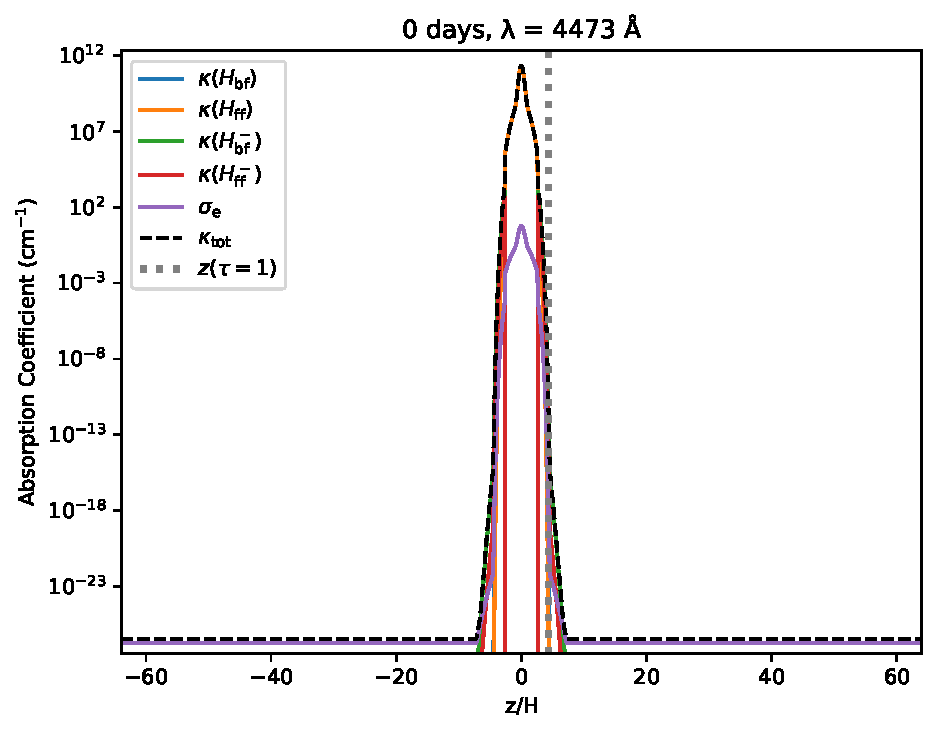
\includegraphics[width=1.0\textwidth]{ch_snrt_figs/opacity_480x480_w4473_0000.pdf}
	\caption[Vertical opacity profiles for initial conditions]{Opacity profiles from model \code{r1e3-z0h} showing contributions from each component in \eq{eqn:total-kappa} for the column passing through the center of the SN for the initial conditions.}
\label{fig:opacity-profile0}
\end{figure}

\begin{figure}
    \centering
    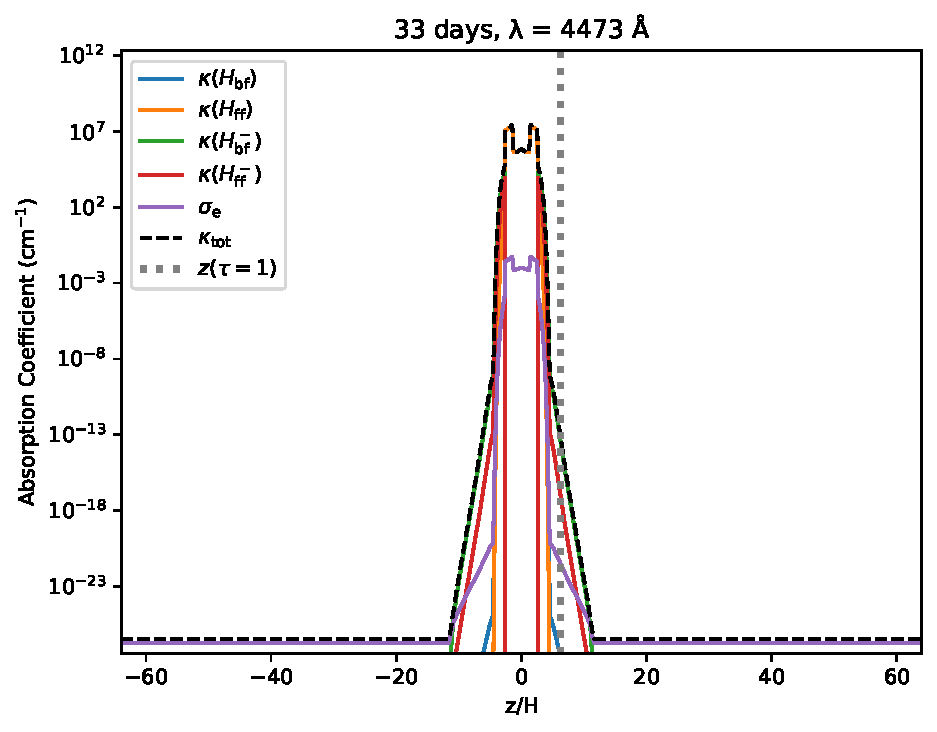
\includegraphics[width=1.0\textwidth]{ch_snrt_figs/opacity_480x480_w4473_0013.pdf}
	\caption[Vertical opacity profiles at shock breakout]{Vertical opacity profiles at shock breakout.}
	\label{fig:opacity-profile13}
\end{figure}

\begin{figure}
    \centering
    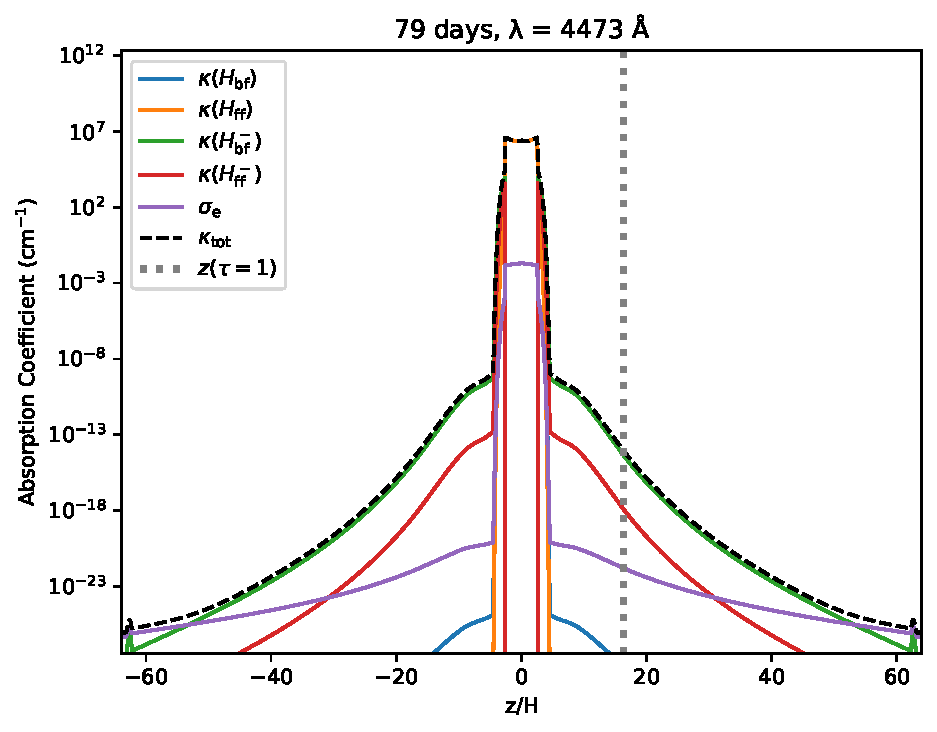
\includegraphics[width=1.0\textwidth]{ch_snrt_figs/opacity_480x480_w4473_0031.pdf}
	\caption[Vertical opacity profiles in final snapshot]{Vertical opacity profiles in the snapshot before the shock leaves the domain.}
	\label{fig:opacity-profile31}
\end{figure}

When the ionization fraction becomes large (i.e., $1 - n_\text{HII}/n_\text{HI}>10^{-2}$), we switch to using the following expression for the free-free absorption component as a function of frequency $\nu$
\begin{equation}
	\kappa_{\nu}(\text{H}_\text{ff}) \rho = \frac{4e^6}{3\, h\, c\, \me^2} \left( \frac{2\pi \me}{3kT} \right)^{1/2} \ \gff\, \nElec\, \nI\, Z^2\, \nu^{-3}\,\left[ 1 - \exp \left(-\frac{h\nu}{kT}\right) \right],
\end{equation}
where
\begin{equation}
    \gff \approx \rm{ln} \bigg( \exp \bigg\{ 5.960 - \frac{\sqrt{3}}{\pi} \ ln \bigg[ \frac{\nu}{10^9\ \rm{Hz}} \bigg( \frac{T}{10^4\ \rm{K}} \bigg)^{-3/2} \bigg] \bigg\} + e \bigg)
\end{equation}
is the Gaunt quantum mechanical correction factor, and the final term $e$ is Napier's constant.
Since this expression is for absorption with units cm$^{-1}$, we take it out of \eq{eqn:total-kappa} and add it directly to our calculation of $\alpha_\lambda$. 

\Fig{fig:opacity-profile0}, \Fig{fig:opacity-profile13}, and \Fig{fig:opacity-profile31} show the opacity profiles for our fiducial model at $R=10^3\,\Rs$ and $z=0H$ for each term in \eq{eqn:total-kappa} for the central wavelength in our range $\lambda=4473\,\text{\AA}$ at the initial conditions, shock breakout, and the snapshot before the shock leaves the $z$ boundary.
The vertical dotted line shows the photosphere ($\tau=1$) when observed from the positive $z$-direction.
At $t=0$ days, the disk midplane is dominated by $\kappa(\text{H}_\text{bf})$ and $\sigma_\text{e}$, but the disk photosphere at $z=5H$ is dominated by free-free absorption from $\kappa(\text{H}_\text{ff})$ and $\kappa(\text{H}_\text{ff}^-)$.
At $t=31$ days when the SN shock passes $z=5H$ and the light curve in \Fig{fig:all_lcs} rises, $\kappa(\text{H}_\text{bf})$ becomes the dominant opacity source.
At $t=76$ days, when the shock reaches the domain boundary, the opacity at the photosphere is still dominated by $\kappa(\Hminus_\text{bf})$ followed by $\kappa(\text{H}_\text{ff})$, which contributes a relatively small amount.

In \Fig{fig:UVIpIm-0}, \Fig{fig:UVIpIm-13}, and \Fig{fig:UVIpIm-31} we show the vertical profiles for the core values calculated with the Feautrier method in the \ocotillo code -- the mean intensity $U$, flux $V$, upward intensity $\Iplus$, and downward intensity $\Iminus$ -- for the same times and wavelength as in \Fig{fig:opacity-profile0}, \Fig{fig:opacity-profile13}, and \Fig{fig:opacity-profile31}, respectively, along the central column that passes through the SN.
The strong bump in the middle of the initial conditions for $U$, $\Iplus$, and $\Iminus$ is generated by the SN perturbation, and the small bump at the base is caused by the accretion disk.
The curve for $V$ represents the flux of energy being passed to the cells on either side of a given point, meaning an observer sees the value at the boundaries.
The center is bright due to the SN, but the flux drops quickly as the disk absorbs the radiation.
Moving further outwards, the radiation is emitted again at the disk edge and streams freely towards the boundaries.
When the shock breaks out at $t=33$ days, $V$ increases until it reaches its maximum when the shock is near the $z$-boundary at $t=79$ days.

\begin{figure}
	\centering
	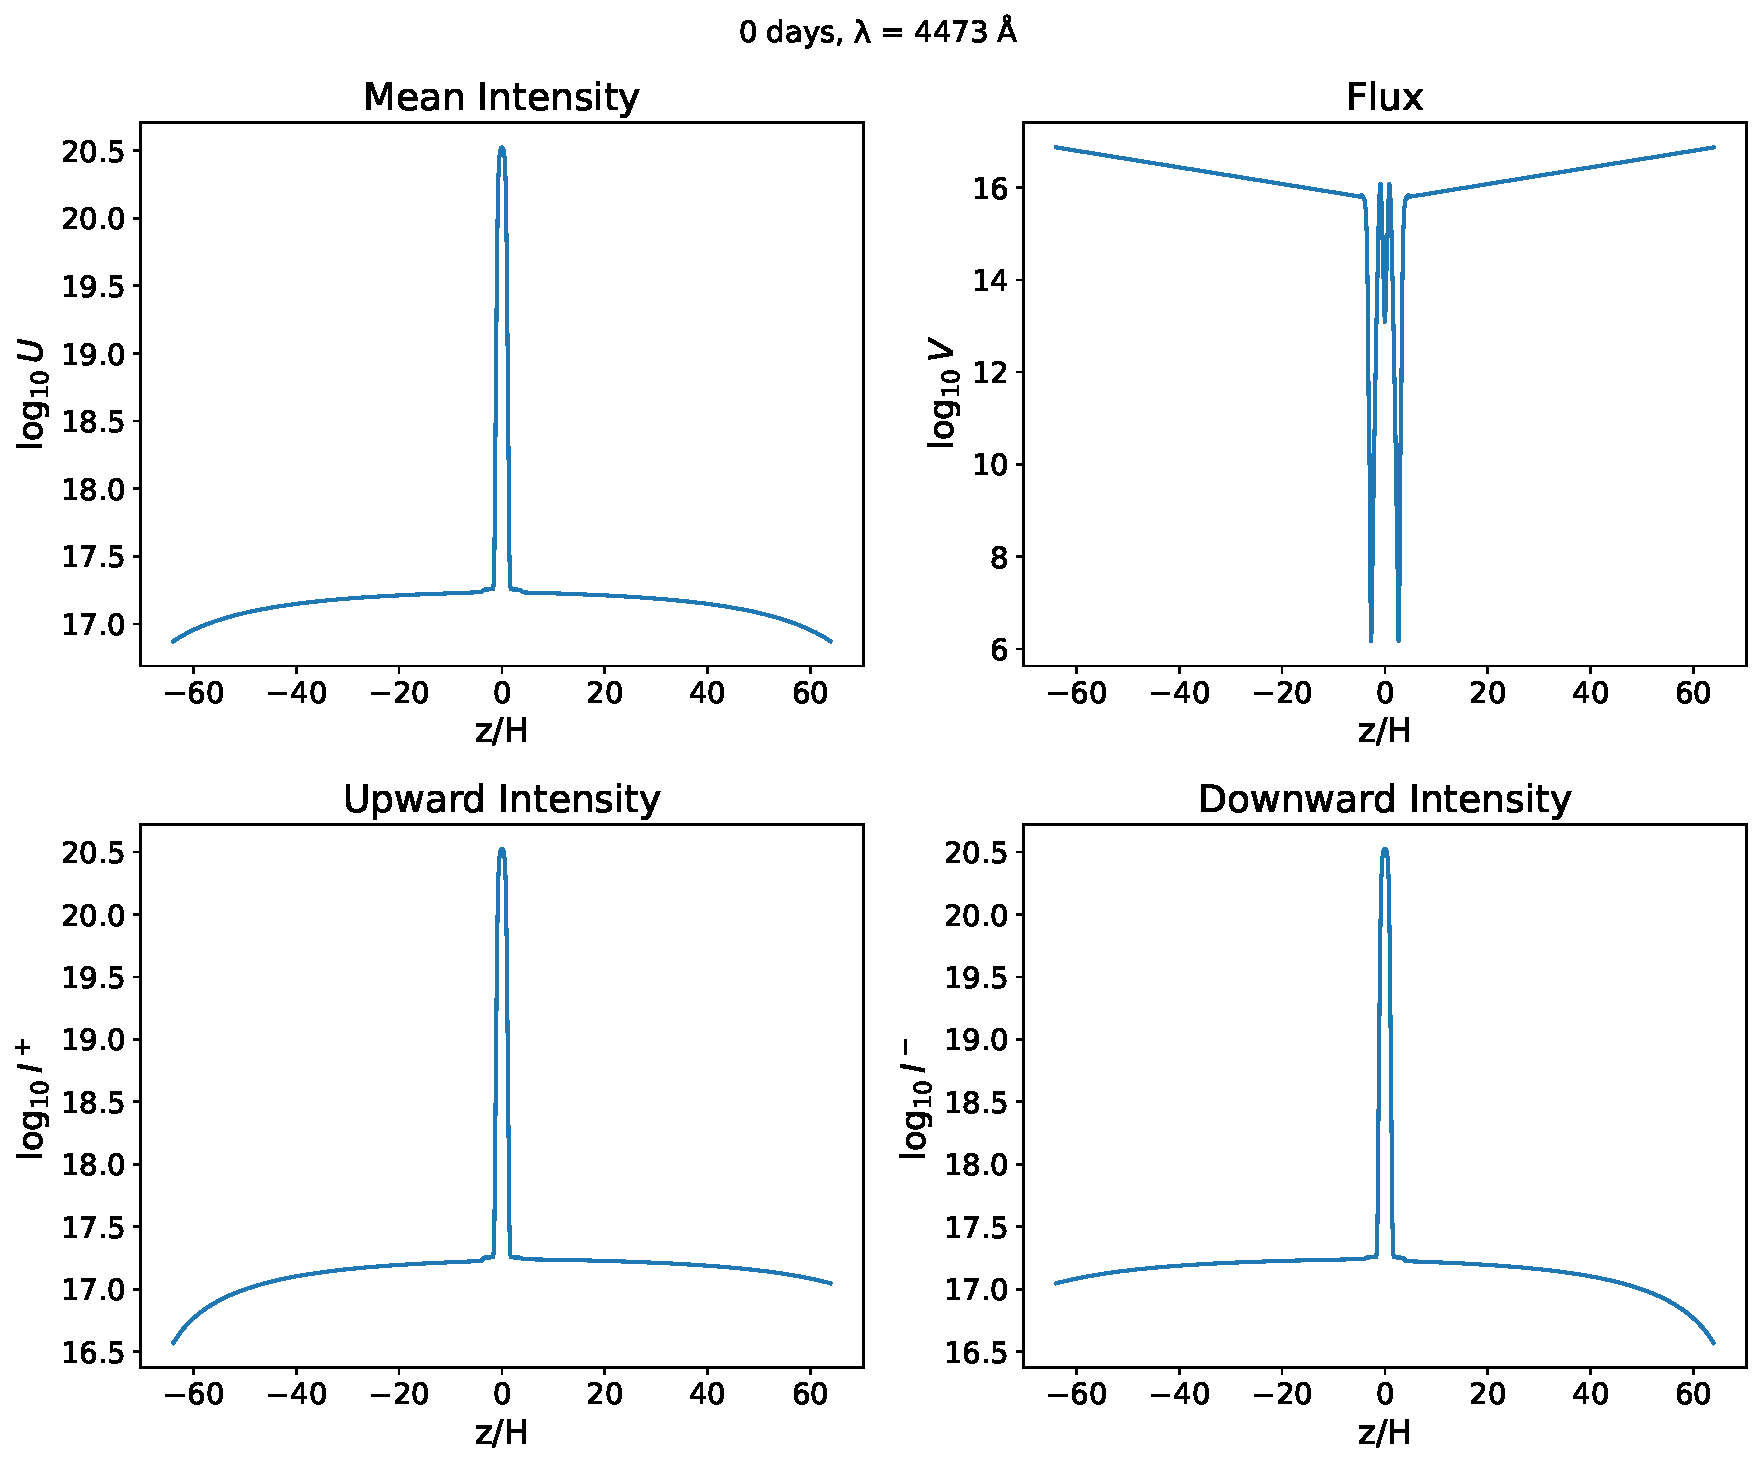
\includegraphics[width=1\textwidth]{ch_snrt_figs/intensity_480x480_w4473_0000.pdf}
	\caption[Feautrier Solutions from \ocotillo for the fiducial model \texttt{r1e3\_z0h} at 0 days]{Feautrier solutions. Mean intensity (upper left), flux (upper right), and upward intensity (lower left), and downward intensity (lower right)when applied to our density and temperature initial conditions for the central wavelength in our array $\lambda=4473\,\text{\AA}$.}
	\label{fig:UVIpIm-0}
\end{figure}

\begin{figure}
	\centering
	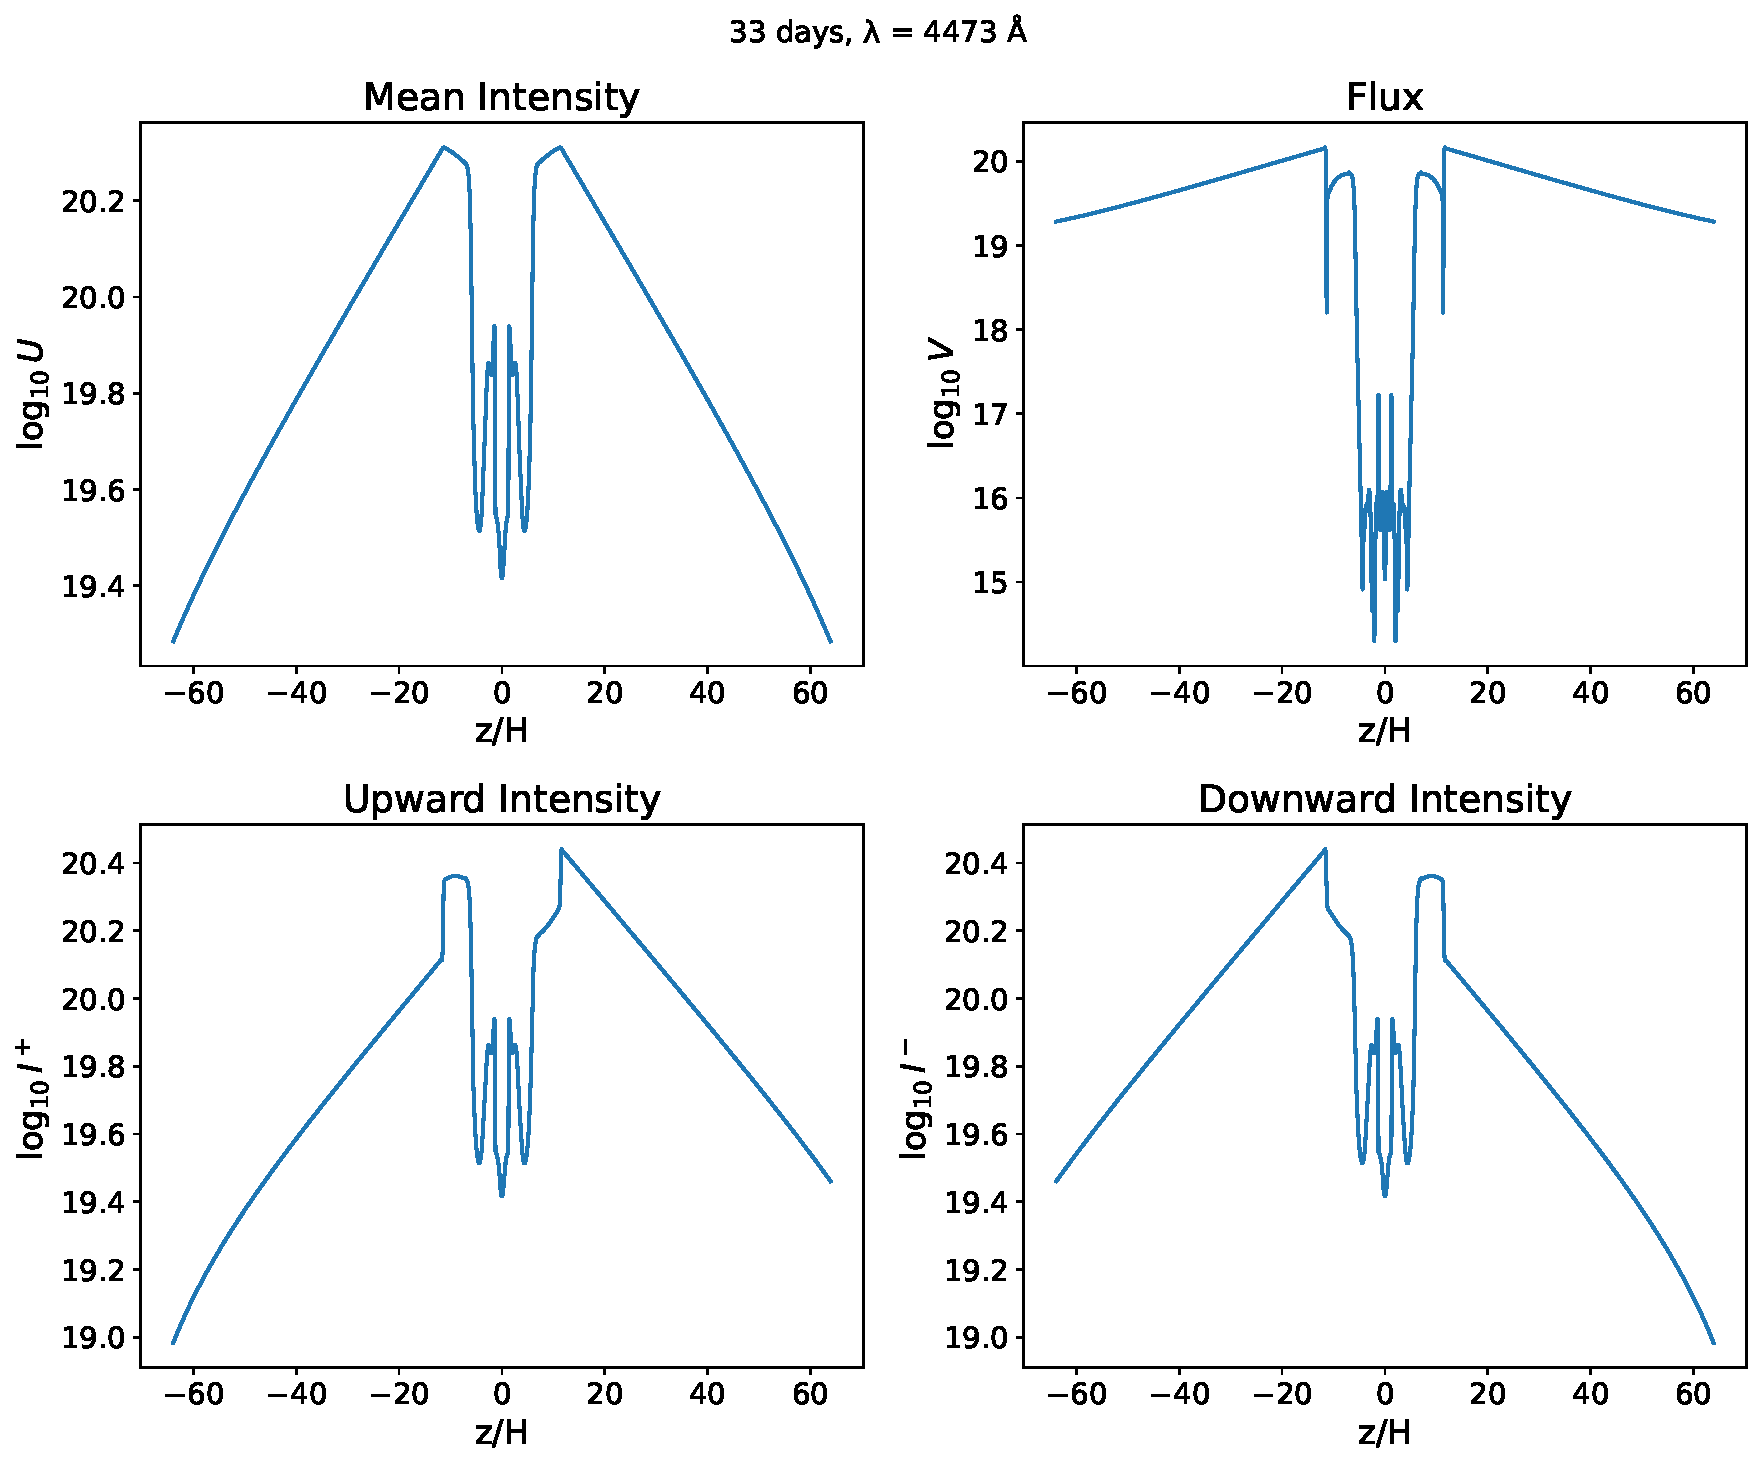
\includegraphics[width=1\textwidth]{ch_snrt_figs/intensity_480x480_w4473_0013.pdf}
	\caption[Feautrier Solutions from \ocotillo for the fiducial model \texttt{r1e3\_z0h} at 33 days]{Mean intensity, flux, and intensity results at shock breakout.}
	\label{fig:UVIpIm-13}
\end{figure}

\begin{figure}
	\centering
	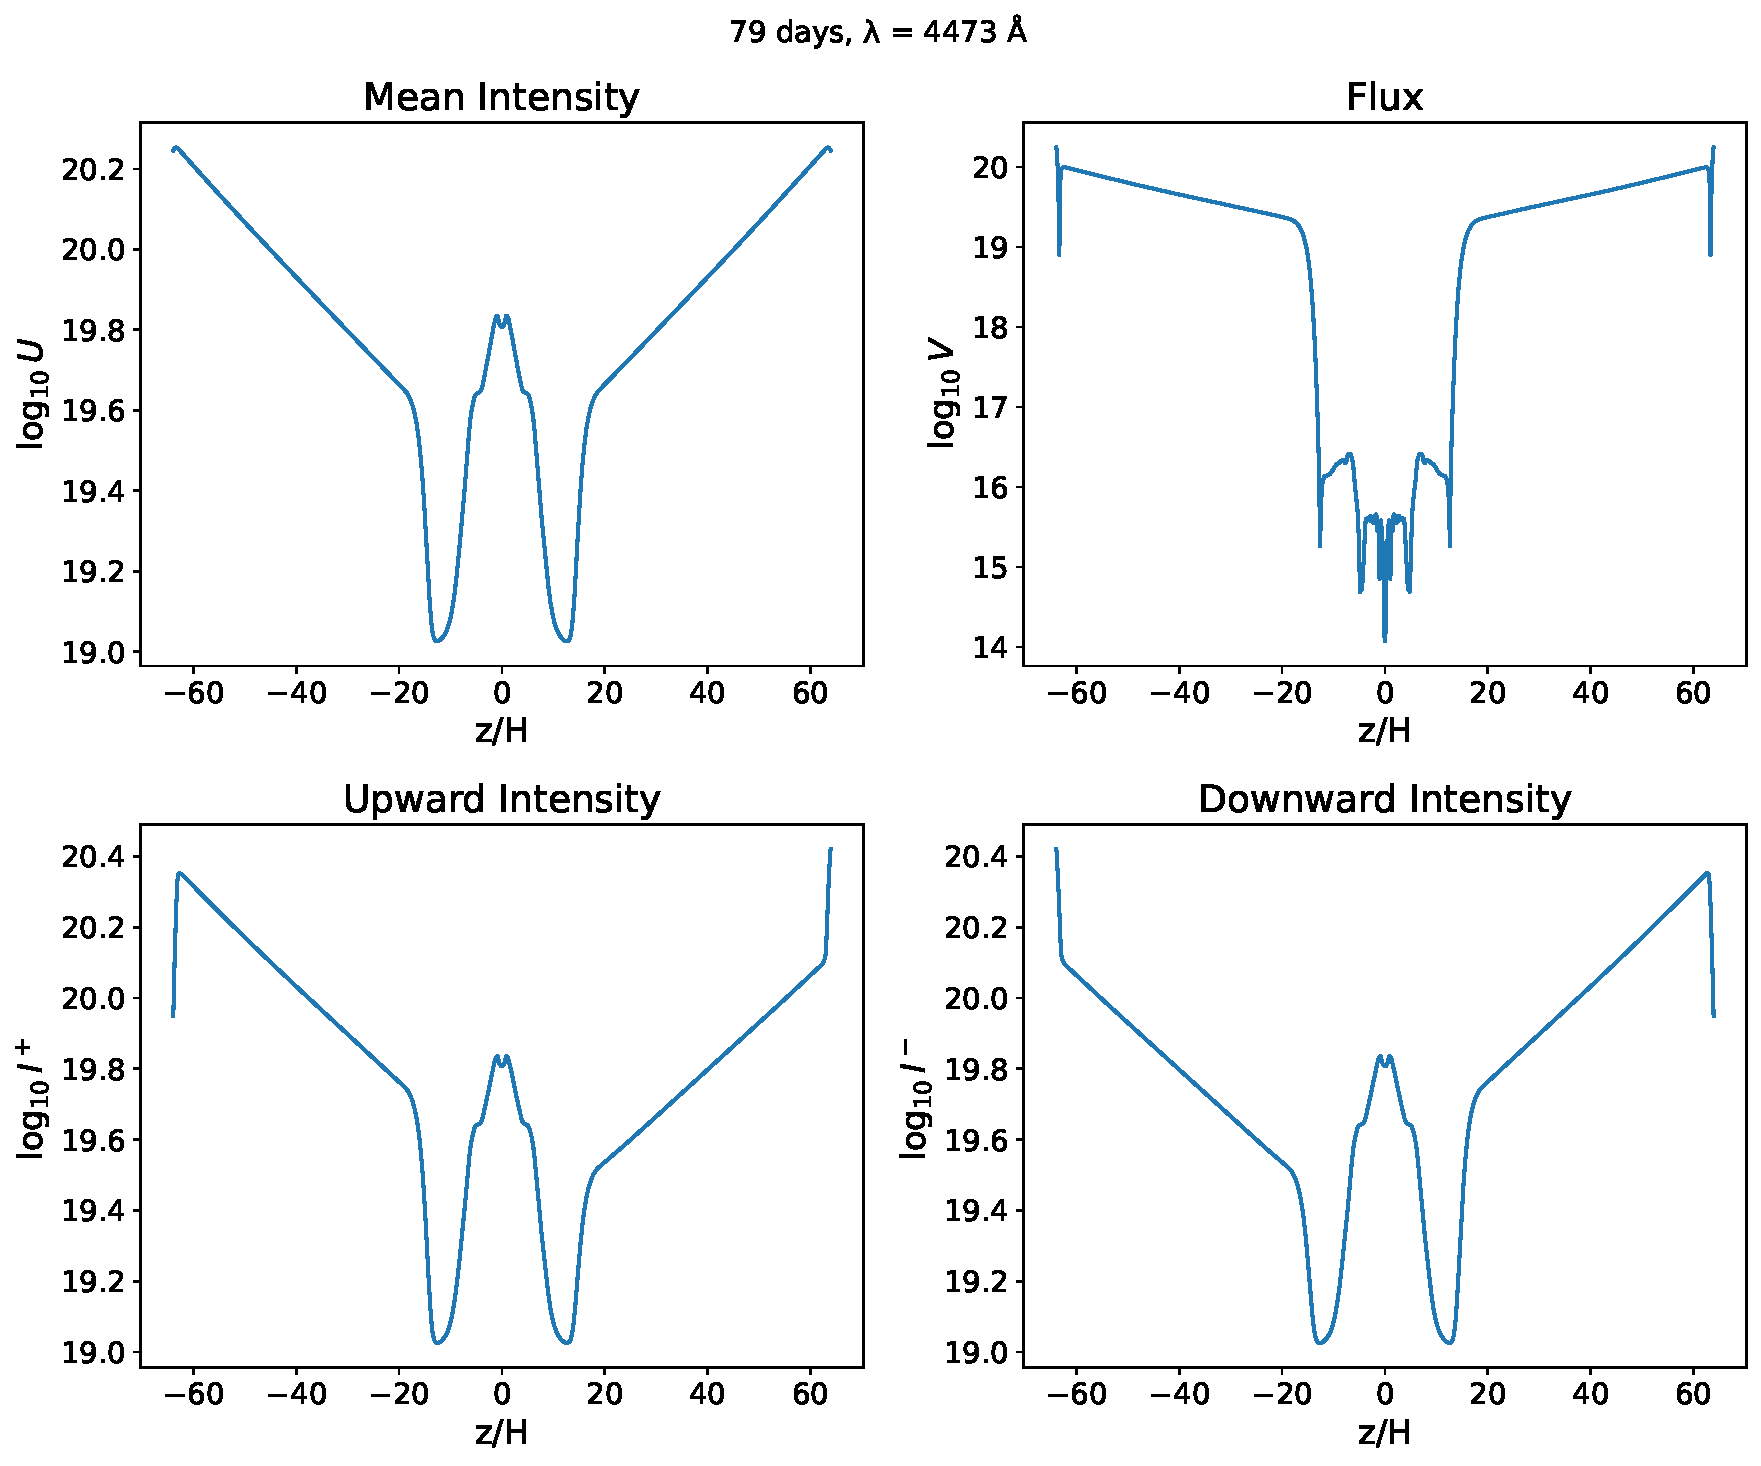
\includegraphics[width=1\textwidth]{ch_snrt_figs/intensity_480x480_w4473_0031.pdf}
	\caption[Feautrier Solutions from \ocotillo for the fiducial model \texttt{r1e3\_z0h} at 79 days]{Mean intensity, flux, and intensity results in the snapshot before the shock leaves the domain.}
	\label{fig:UVIpIm-31}
\end{figure}


\subsection{Results} \label{sec:results}

\subsubsection{Fiducial Model} \label{sec:fiducial-results}

The \citet{SirkoGoodman03} disk has the highest volume density at $10^3\,\Rs$ where we place our fiducial miplane model \code{r1e3-z0h}.
This location was also chosen because it is the most optically thick and thus most likely to prevent or delay electromagnetic radiation from reaching the disk photosphere.
Using \eq{eqn:temp-profile} to apply the temperature profile, we set $\Tmid=6\times10^4$ K.
The blue curve in Fig.~\ref{fig:all_lcs} is the light curve calculated using our post-processing radiative transfer code \ocotillo
%\ref{sec:Appendix-RTModel})/
after integrating the flux over 50 wavelengths over the range $800\leq\lambda\leq8000\ \text{\AA}$.
The light curve remains constant for the first $\sim$20 days when the shock begins to pass through the disk's photosphere and breaks free at $\sim$30 days.
The luminosity rises to $10^{46}\,{\rm erg\,s}^{-1}$ over the next 50 days as the shock expands outside the disk, peaking at $\sim90$ days.
The kink in the light curve at this time is due to the shock crossing the $z$-boundary, meaning we do not capture the true peak of the lightcurve.
However, continuing their curves, we can estimate their peaks will occur at 115 days emitting $2\times10^{47}\,\text{erg s}^{-1}$ (\code{r1e3-z1h-up}) and at 140 days emitting $3\times10^{46}\,\text{erg s}^{-1}$ (\code{r1e3-z0h}).

\begin{figure}[htbp]
    \begin{subfigure}{0.5\textwidth}
        \centering
        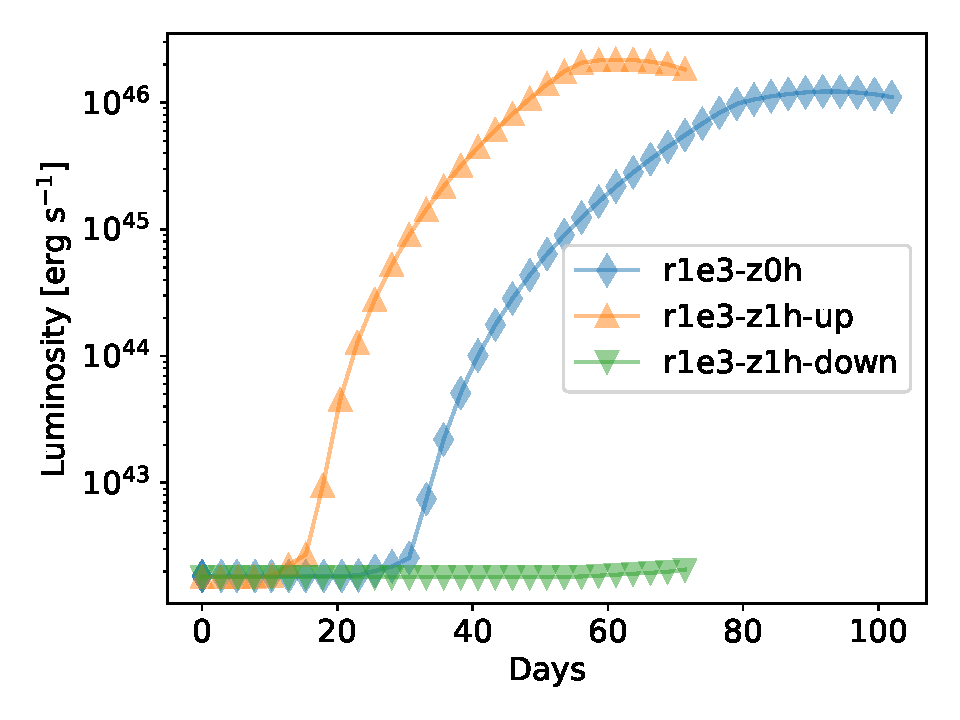
\includegraphics[width=1\linewidth]{ch_snrt_figs/lightcurves_r3.pdf}
    \end{subfigure}
    \begin{subfigure}{0.5\textwidth}
	\centering
        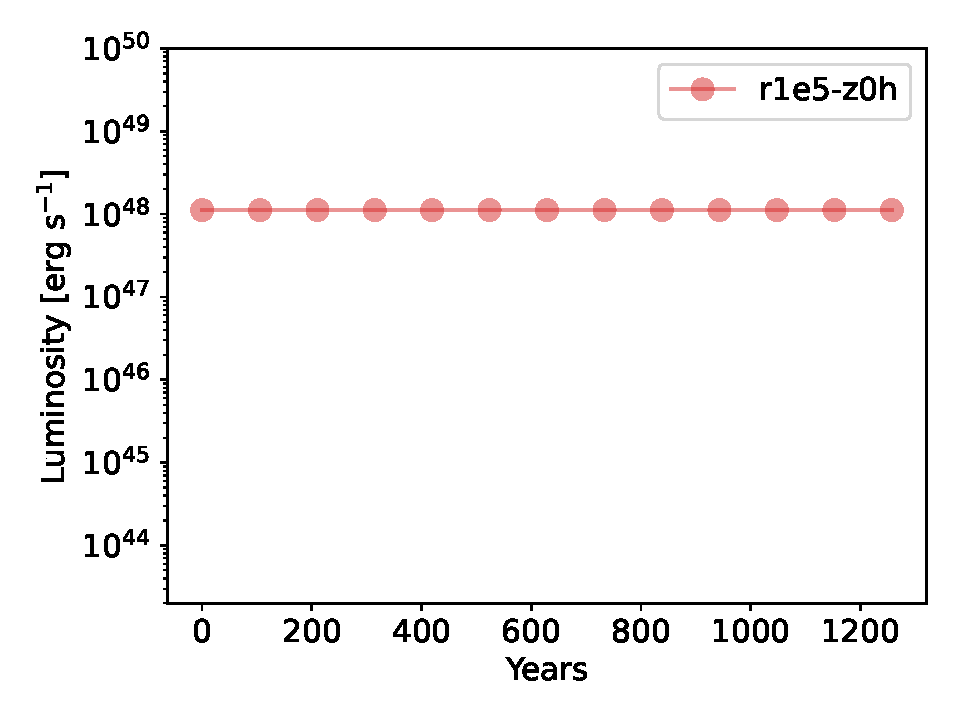
\includegraphics[width=1\linewidth]{ch_snrt_figs/lightcurves_r5.pdf}
    \end{subfigure}
	\caption[Optical light curves]{\textbf{Optical light curves} for our SN simulations integrated over 50 wavelength bins spanning 800 to 8000 $\text{\AA}$.
	\code{r1e3-z0h} is our midplane fiducial model at $r=10^3\,\Rs$, \code{r1e3-z1h} is our model at the same radius but with the SN placed at a height $z=1\,H$.
	The curve labeled with \code{-up} is produced when observing from the positive $z$ boundary (i.e., the same side of the midplane as the offset SN), while the curve labeled with a \code{-down} is produced when observing from the negative $z$ boundary, or the far side of the disk.
	The lower panel shows the lightcurve from our \code{r1e5-z0h} model which places a midplane SN at $r=10^5\,\Rs$.
    % The radiation from the midplane supernova (solid line) escapes the optically thick disk after $\sim$30 days, and the luminosity rises over the next 60 days and peaks at $10^{46}$ erg s$^{-1}$. 
    }
    \label{fig:all_lcs}
\end{figure}

\subsubsection{Offset Model}

Our model where the SN is placed at $z=1\,H$ produces two different light curves when viewed from opposite sides of the disk.
When viewed from the same side of the midplane as the SN (model \code{r1e3-z1h-up}) the orange light curve exhibits changes earlier than the default midplane case, corresponding to the shorter time it takes the shock to reach the disk photosphere.
Now, the radiation escapes at $\sim15$ days and rises faster than the midplane case in \code{r1e3-z0h} to a peak twice as bright.
Viewing from the far side of the disk (model \code{r1e3-z1h-down}), the green light curve shows no change except for a slight brightening when the flow reaches the disk photosphere near $\sim60$ days.

\subsubsection{SNe in the Outer Disk}

The right panel of Fig.~\ref{fig:all_lcs} shows the lightcurve for model \code{r1e5-z0h} where a midplane SN is placed at $r=10^5\,\Rs$.
In Paper I, the shock from this SN did not break free from the disk, and we see that the light curve similarly remains constant.
The baseline luminosity for the disk in this lightcurve is higher than the other light curves due to the hotter effective temperature of the disk at $r=10^5\,\Rs$. 

% Text for the color evolutions.
% The right panel shows the color evolution when comparing the central wavelengths in the $g$ and $r$ filter bands. The color becomes bluer as the bright shock dominates the dimmer disk. However, the color only changes by 0.04 -- well within the scatter of the ZTF data for AGN J1249$+$344.


\subsubsection{Color Evolution}
SNe are often classified and identified by their color evolution.
We integrate the flux emitted by our models over the wavelength ranges corresponding to the ZTF $g$ and $r$ band filters and calculate the $g-r$ color evolutions with:
\begin{align}
	F_{i} &= \int_{\lambda_{i}^0} ^{\lambda_{i}^1} F_\lambda d\lambda \\
	g-r     &= -2.5\log_{10}\frac{F_g}{F_r}
\end{align}

\Fig{fig:color-lightcurve} shows the color evolution for each of the models.
For models \code{r1e3-z0h} and \code{r1e3-z1h-up}, the color becomes slightly bluer when the hot shock emerges and remains constant as the ejected material expands.
Meanwhile, models \code{r1e3-z1h-up} and \code{r1e5-z0h} do not appreciably change color, mimicking their light curves, but \code{r1e3-z0h-down} does slightly change as the subsonic flow breaks through to the far side.
Even though two models showed color changes, the difference is small $\Delta (g-r)=0.04$ and would not have been detectable against the variability in AGN J1249$+$344 ($\Delta(g-r)\sim0.1$) if alert ZTF19abanrhr had been caused by a SN.

\begin{figure}
    \centering
    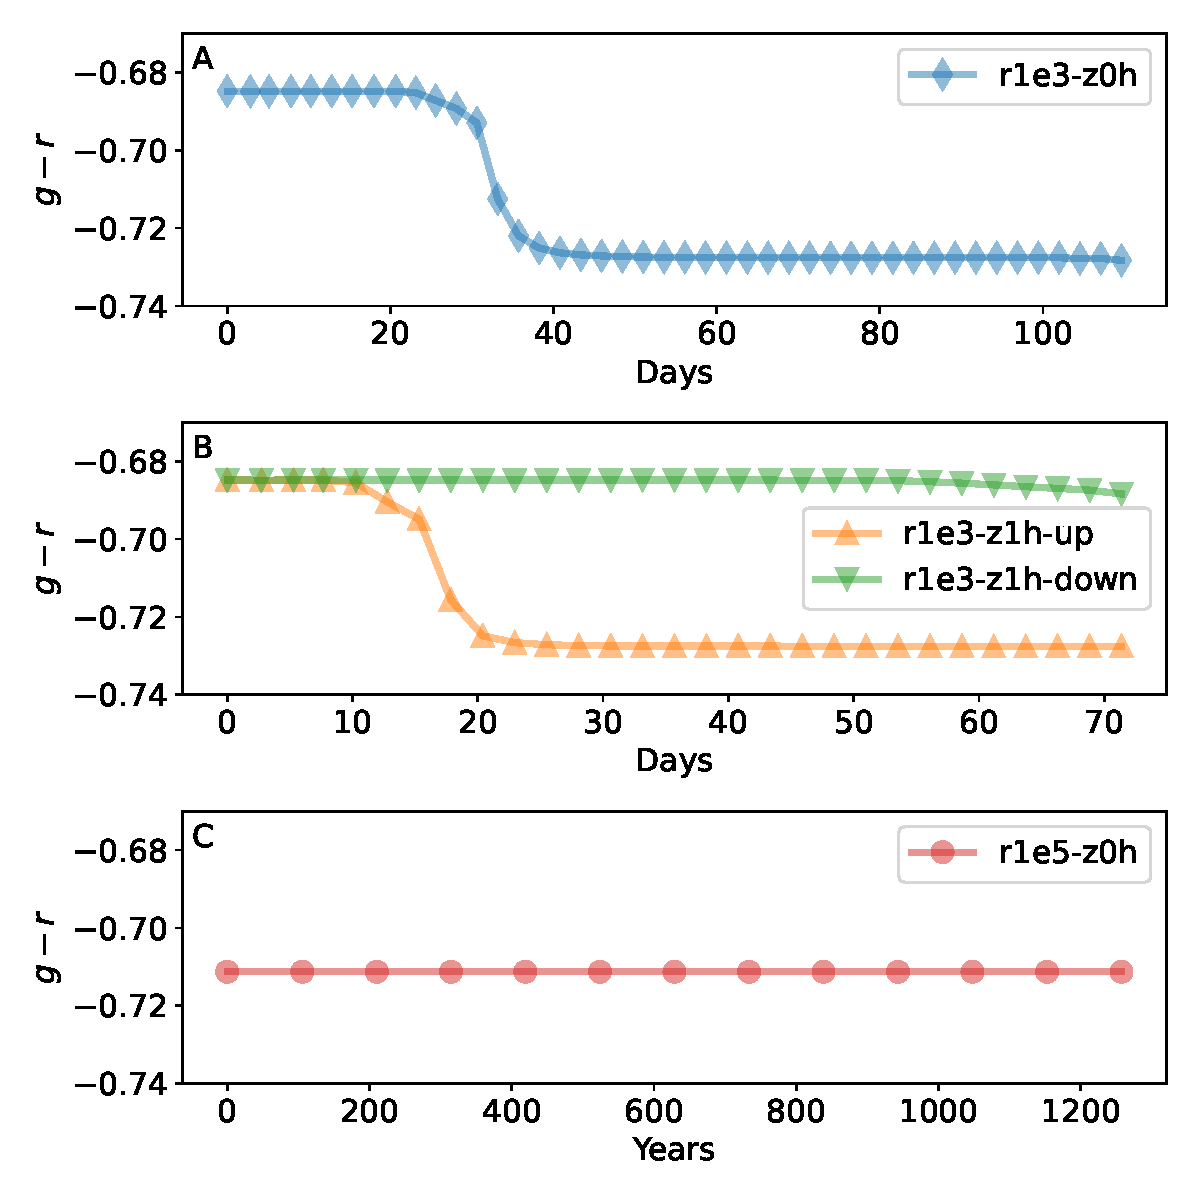
\includegraphics[width=1.0\columnwidth]{ch_snrt_figs/gr_color_composite.pdf}
	\caption[ZTF $g-r$ color evolutions]{ZTF $g-r$ color evolutions. Panel A is from our fiducial model at $R=10^3\,\Rs$, panel B is the offset model at the same radius, and panel C is the midplane model at $R=10^5\,\Rs$.
    The observed color becomes bluer when the shock breaks free, but the small change $\Delta(g-r)\sim 0.04$ would be undetectable amidst the noise for AGN J1249$+$344 with $\Delta(g-r)\sim0.1$ as reported by \citet{Graham+20}.}
    \label{fig:color-lightcurve}
\end{figure}


% \subsection{Magnitudes and Colors} \label{subsec:Mags+Colors}


% According to the methods described in the previous subsection, we derived a multi-wavelength flux $F_\lambda$ from our simulation. In order to compare them with the lightcurves quoted in \citet{Graham+20}, we convert the flux into apparent magnitudes.
% $F_\lambda$ is the value observed by a telescope placed directly at the z-boundary of the computational domain, so we convert these to apparent magnitudes for a source in AGN J124942.3 $+$ 344929 at $z=0.438$ or ~2.4 Gpc \citep{Graham+20}.

% To calculate a bandpass magnitude requires the zero point. ZTF filters are calibrated to match the Pan-STARRS 1 filters according to the release paper \citep{Bellm+19}. Magnitudes in this system follow the "monochromatic AB magnitudes" (Oke \& Gunn 1983)

% \begin{align}
% m_{\rm ABNU}(\nu) &= -2.5\log(f_\nu/3631\ {\rm Jy}) \\ 
%             &= -48.6 -2.5\log(f_\nu[{\rm erg/sec/cm}^2{\rm /Hz}])
% \end{align}
% \citet{Schlafly+12} reported zero points of $g_{\rm ZP}=24.41$ and $r_{\rm ZP}=24.68$, which we can use to calibrate the flux to those of the observations in \citet{Graham+20}.

\subsection{Discussion} \label{sec:discussion}

The baseline disk luminosities in Fig.~\ref{fig:all_lcs} are only produced by the radiation emitted by the small patch of the disk contained in the shearing box models, whereas the full integrated disk luminosity is much larger.
While studying spectra for AGN accretion disks, \citet{Hubeny+01} found that a disk around a black hole of mass $\Mbh=10^8\,\Msun$ has a luminosity $L=0.3L_\text{Edd}=4.4\times10^{45}(M/\Msun)$ erg s$^{-1}$ when considering electron scattering and a viscocity parameter of $\alpha=0.01$ .
Therefore, only the SNe in models \texttt{r1e3-z0h} and \texttt{r1e3-z1h-up} may be detectable against the bright disk, and any observations would need to be able to distinguish changes from the disk emission by a factor of a few.
Additionally, as shown in \Fig{fig:color-lightcurve}, the color changes for these two SNe are very small ($\Delta g-r \sim 0.04$).



Comparing with alert ZTF19abanrhr, the proposed EM counterpart to GW190521, our lightcurves are similarly energetic, and exhibit the same lack of color evolution.
Therefore, an AGN-SN may be indistinguishable from a flare caused by the recoiling remnant of a BBH merger that generates a shock in the disk \citep{McKernan+19}. 
Future work should model the black hole recoil to identify distinguishing characteristics between the two events.

While the light curves do begin to level out, the peaks we see in the \code{r1e3-z0h} and \code{r1e3-z1h-up} curves in \Fig{fig:all_lcs} are artificially caused by the shock passing through the $z$ boundaries.
We cannot push our domain size larger using the current grid structure due to resolution limitations without needing non-equidistant grids,  mesh refinement, or global simulations in polar coordinates.
Also, our radiative transfer model is limited to one dimension, and therefore cannot account for scattering at oblique angles to the line of sight.
As such, the mean intensity may change due to this effect, but we have performed these calculations with a face-on view of the disk which is expected to be the brightest viewing angle.
However, massive stars in the disk may not detonate as SNe at all.
The disk is a large reservoir of hydrogen fuel that continuously replenishes the star's supply if it is sufficiently embedded in the disk.
\citet{CantielloJermynLin21} showed that stars can reach masses of $M\approx300\,\Msun$, easily passing through the so-called pair-instability mass gap that spans $60\lesssim M \lesssim 160\,\Msun$ \citep{WoosleyHeger21}.
Stars that reach these masses will need to expel much more massive envelopes that could significantly delay their shock breakout from the disk or turn it into a subsonic flow entirely.
Thus massive stars that do finally fuse iron in their cores while embedded in an AGN disk will likely not evolve the same as those that lived their lives in the field away from such a plentiful resource.

%\begin{itemize}
%    \item observable against AGN disk luminosity? (draw line next to LCs?)
%    \item how do SNe impact broad line region (BLR) of AGN?
 %   \item Are repeated SNe required to physically perturb the disk enough for the  BLR to change (check paper I for discussions of the broadline region)?
 %   \item can SNe create hot spots that result in BLR variability?
 %   \item rates of these SNe given the star formation rate in the outer disk \citep{SirkoGoodman03, DittmanMiller20} and disk capture \citep{Fabj20}. Need to consider that stars possibly evolve differently in AGN due to its large fuel reservoir \citep{Cantiello21}.
%\end{itemize}


\subsection{Conclusions} \label{sec:conclusion}

We performed post-processing radiative transfer calculations on hydrodynamic shearing box calculations of SNe embedded in AGN disks.
By implementing the Feautrier method we calculated the absorption and scattering processes caused by hydrogen atoms and free electrons.

For SNe at the midplane in the inner disk ($r=10^3\,Rs$), the radiation emerges $\sim30$ days later and rises quickly to a peak at $L=10^{46}\ \text{erg s}^{-1}$.
Typical AGN luminosities can be $\mathcal{O}(10^{43}-10^{48}\ \text{erg s}^{-1})$, so these SNe will only be brighter than AGN of $L\ll10^{46}\,\text{erg s}^{-1}$, which is the range for Seyfert galaxies and other low-luminosity AGN, and will not be visible in quasars.
Radiation from a SN at the same location but offset from the midplane at $z=1\,H$ emerges 15 days earlier, rises much faster, with a luminosity that peaks at $2 \times 10^{46}\,\text{erg s}^{-1}$ when viewed from the same side of the midplane.
The radiation does not reach the other side of the disk in a detectable manner under this scenario.
While bright, these SNe may not be detectable against a bright AGN disk, but would be easily seen if occurring in a starved disk or during an episode of lower mass accretion rates.
For SNe detonating in the outer disk at $r=10^5\,\Rs$, the large scale height of the disk prevents the hot shock from emerging from the photosphere.

Embedded SNe do not exhibit a significant color evolution.
Without this key indicator that is common to naked SNe, they may be indistinguishable from flares produced by recoiling BBH merger remnants.
As such we will need to consider a different part of the spectrum or aspects of these transients to reliably distinguish between flares emitted by embedded merger remnants versus embedded SNe in transient searches such as ZTF or LSST and their archives.



\clearpage
\resetcounters
\addtocontents{toc}{\protect}
\section{\texorpdfstring{\MakeUppercase{future work and perspectives}}{future work and perspectives}}
\label{sec:chapter-future}

\counterwithin{figure}{section}
\counterwithin{table}{section}


\subsection{Updates to McFACTS}
\texttt{McFACTS} is designed to be public, modular and adaptable.
The content presented in this dissertation was performed using \code{v0.3.0}, but we have already implemented stars into the disk (Nathaniel et al. 2026 in prep.) in \code{v0.4.0}.
Other future near-term goals include:
(i) add objects other than BH and main-sequence stars to the disk (neutron stars, white dwarfs)
(ii) consider the EM significance of encounters between objects (including TDEs, partial TDEs, GRBs as well as disk-crossing events),
(iii) treat the final time step of mergers with increasing sophistication, including calculating details of eccentricity evolution, recoil kicks from numerical relativity calculations (Ray et al. 2026 in prep.) and disk re-capture correctly,
(iv) allow multiple AGN episodes to occur in a given nucleus, with appropriate dynamical relaxation, (v) predict the rate and magnitude of optical/ultraviolet/X-ray flaring due to explosive events \citep[mergers, disk-crossings, SNe, TDEs,][]{McPike+26-mcfactsIV},
(vi) develop and add new models of AGN disks to reflect recent simulations \citep{Hopkins+24}, and
(vii) add more sophisticated treatments for binary capture \citep{Whitehead+25b} and stalling of gas hardening (Postiglione et al. 2026 in prep.).

\subsection{Updates to Ocotillo and New Models}


The embedded SNe light curve we produced was marginally visible against a bright AGN disk and the color evolution would likely be lost in the noise of typical AGN variability. 
However, we did not capture the peak of the light curve due to domain size limitations with our uniform grid.
Future studies should move to a code that supports adaptive mesh refinement or static mesh refinement at a minimum since we are approaching the limits of resolution for three-dimensional uniform grids in terms of computational expense and data storage requirements.
Additionally, we will likely need to move to a global disk model that will enable us to model the full disk emission.
Codes like \citep[\code{Athena++}][]{Stone+20} may be appropriate for this purpose.

Ocotillo will need an upgrade to calculate in three dimensions for a global disk in spherical coordinates that spans the full meridional domain rather than one with boundaries just above and below the disk.
We will also expand its treatment for the gas composition to achieve ionization states for a broader range of atomic species that more accurately reflect the solar and super-solar metallicities found in AGN \citep{HuangLinShields23}, requiring additional opacities starting with helium.


We also plan to model the hydrodynamics and radiative transfer of a recoiling BBH merger remnant.
In a black hole merger, some mass is lost and converted into gravitational waves, dissipating energy and angular momentum; a loss that is accompanied by a decrease of the Hill radius of the remnant in comparison with the combined Hill radius of the progenitors.
The dynamical consequences are manifold.
First, gas within the Hill sphere that is orbiting too fast for the new lower mass moves outward, self-colliding \citep{McKernan+19}.
Second, gas no longer bound by the new, smaller Hill sphere shocks with AGN gas in orbit around the central mass.
Third, a gravitational wave kick at merger causes ram-pressure stripping of the original Hill sphere gas as it collides with a comparable mass of disk gas.
Flares from disk-remnant interactions have been studied analytically \citep{McKernan+19}, showing that whether the flare is prompt or delayed depends on whether the Hill sphere radius is larger than (prompt ultraviolet and optical flare) or smaller than (delayed and diminished with drawn out optical flare) the disk scale height.
Our proposed work will test these analytical results and produce theoretical observables for comparison with follow-up campaigns to future gravitational wave detections, shedding light onto a problem that has received little numerical attention \citep{Corrales+10}.
To model these disk-remnant interactions, we will also need to move to a code with static or adaptive mesh refinement for a global model.
We will represent the recoiling black hole by giving a velocity kick to the portion of
the disk gas within its Hill sphere directed along a chosen trajectory while varying the direction and kick velocity.
This construction eliminates the need for a domain large enough to contain the remnant’s
entire orbital path, and focuses computational resources on the disk-remnant interaction that occurs
over a short timescale in a localized region of the disk.



\clearpage

% Below is for an appendix or appendices if you have them. If not just comment it all out

%\pagestyle{empty}  % No page number on the half-title appendix page...okie dokie can do nmsu. (Note the page number count still increases, we're just printing the page number on the page.)

%\begin{center}
%APPENDICES
% NMSU requires a half-title page that is labeled APPENDIX or APPENDICES (depending if you have 1 or 2+ appendix/appendices.) Yes, literally a whole page with nothing but this word, cause ya know, that makes sense...
%\end{center}

%\addtocontents{toc}{\protect\contentsline{}{}{}}  % Add an extra line before 'Appendices' in the table of contents
%\appendix % Start the appendix

%\clearpage
%\resetcounters

%\etocsettocdepth.toc {section}

%\pagestyle{plain}  % Resume printing page numbers

%\clearpage
%\resetcounters
%\addtocontents{toc}{\protect}
\section{\texorpdfstring{\MakeUppercase{the mcfacts code: monte carlo method for black hole mergers in agn disks}}{the mcfacts code: monte carlo method for black hole mergers in agn disks}}
\label{sec:apdx-mcfacts}

\counterwithin{figure}{section}
\counterwithin{table}{section}

The contents of this appendix was published in \citet{McKernan+25-mcfactsI}. Please use that reference when citing this section.

Fig.~\ref{fig:overview} gives a basic overview of the flow of BH through categories in \code{McFACTS}, starting from an initial eccentric BH population of singleton BH in the AGN disk (top left).
Solid arrows indicate a flow from one category to another and dotted arrows indicate influence from one category on another.
For example, there is a flow from the initial eccentric BH population into the circularized BH population via gas damping (blue solid arrow), but the eccentric BH population also dynamically interacts with the circularized population (dotted red arrow) and can excite it to reverse the flow (solid red arrow).
Binary BH are formed from among the circularized population (connecting solid red arrow).
BBH, once formed can dynamically interact with both the eccentric and circularized single BH and the spheroid population (the three dotted red arrows onto Binary BH in Fig.~\ref{fig:overview}).
BBH can flow to softer BBH and ionize, via dynamics (solid red arrows) returning their components back to the eccentric disk BH population, but BBH can also harden via gas and dynamics (blue and red arrows) and ultimately merge, whereupon they either flow back into the eccentric BH population or into the spheroid (from where they can be re-captured generally circularized).
A small sub-population of the initial eccentric population and the spheroid population can flow into the inner disk, where some BH can decay via GW emission and become EMRIs (blue box).
\begin{figure*}
	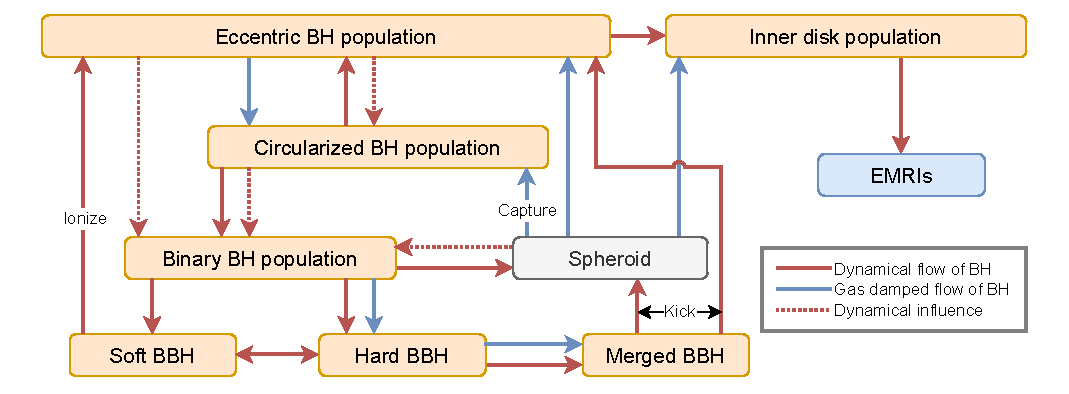
\includegraphics[width=1\textwidth]{appdx_figs/McFacts_flowchart.pdf}
	\caption[Flow diagram of BH categorization in \code{McFACTS}]{Flow diagram indicating how BH are categorized in \texttt{McFACTS} and how BH are exchanged between these categories. Solid arrows indicate a flow of objects from one category to another and dotted arrows indicate an influence of one category on another. Red denotes dynamics, blue denotes gas. Objects in orange (grey) boxes are in the disk (spheroid). EMRIs are in the blue box. For example, there is a flow from the initially eccentric BH population to the circularized BH population due to gas damping (blue arrow), but the eccentric BH population also has a dynamical influence on the circularized BH population (red dotted line) leading to a reverse flow (red solid line). 
    }
    \label{fig:overview}
\end{figure*}

Objects in their disks have their physical parameters manipulated in a consistent algorithmic manner via the \verb|AGNObject| class.
This class will be extended from just BH to stars, neutron stars, and white dwarfs in future updates to the code.
Each \verb|AGNObject| is given a unique ID number, stored in an instance of the \verb|AGNFilingCabinet| class, along with other parameters such as the object's mass and location in the AGN disk.
This allows the code to iterate over the entire population of disk objects when calculating e.g. interactions and binary formation, rather than separating and evaluating objects by type for each iteration.

\subsection{Initial conditions and other inputs}
There are three basic inputs for any simulated galactic nucleus: the SMBH, the NSC, and the AGN disk.
The initial conditions for each of these is set via an input file, for which a default file is provided, or constructed by the user (see Table~\ref{tab:default_model} for \code{p1_default_model.ini}).
Primary input parameters are the SMBH mass ($M_{\rm SMBH}$), the NSC mass ($M_{\rm NSC}$) and the AGN disk model type---users may choose from either a \cite{SirkoGoodman03} or \cite{ThompsonQuataertMurray05} type disk, as implemented in the \code{pAGN} package \citep{Gangardt+24-pAGN} (and for which the user must also specify the disk $\alpha$ parameter, mass accretion rate, $\dot{m}$, and radiative efficiency $\eta$), or may supply their own disk model if they can provide tabulated surface density ($\Sigma$), aspect ratio ($h/r$), and opacity ($\tau$) profiles as a function of disk radius (subject to the requirement that a user-supplied model must be interpolatable over the range of disk radii under consideration, see also below).
A simplified implementation of both the \cite{SirkoGoodman03} and \cite{ThompsonQuataertMurray05} disk models which assumes constant opacity is also provided in \code{McFACTS} along with the pAGN implementation.

We do not currently consider the spin of the SMBH, so there are no input parameters related to it.
However the NSC and the AGN disk have a number of important additional parameters that the user can specify (or use the defaults provided).
Given $M_{\rm NSC}$ and a disk model, we determine (purely based on geometry) the number of stellar mass black holes with orbits fully embedded in the AGN disk at the time the AGN disk initially arrives in the nucleus (here we make the simplifying assumption that the disk does not evolve through the simulation, appearing instantaneously at time zero, subsequently vanishing instantaneously at time $\tau_{\rm AGN}$, the lifetime of the AGN disk, also specified in the input file).
The remainder of the NSC parameters are for distribution functions from which we select the actual objects included in a given simulation for each galaxy.
The user can specify a random number seed (\code{SEED}) in the \code{Makefile} or take the default (in either case the value is recorded for reproducibility).
If the user is simulating multiple galaxies with the same input parameters (the usual mode of operation, in order to build up statistics), each new galaxy will (by default) iterate the original random seed by one, ensuring an entire suite of simulations can be easily reproduced from a starting \code{SEED} and \code{.ini} file.

The \code{SEED} is used to generate initially embedded stellar black hole (BH) masses, orbital semi-major axes ($a$), eccentricities ($e$), inclinations ($i$), arguments of periapse ($\omega$), spin magnitude ($\chi$), and spin angle ($\theta$) from initial distributions set by the \code{.ini} file.
BH masses are drawn from an initial mass function (IMF), assumed to be a Pareto function with a mode mass and powerlaw slope, each of which the user can specify in the \code{.ini} file.
An additional mass feature can be added to the IMF by piling up masses drawn from the powerlaw IMF beyond some maximum mass in a user specified Gaussian distribution.
In this way we can emulate a possible pair instability supernova (PISN) bump in the BH IMF, as physically expected from models of stellar evolution \citep[e.g.][]{RenzoSmith24}, as well as a mass pile-up in the LVK observations \citep{Abbott+23-massbump}.
BH number density is set by the NSC model and default is a broken power-law distribution consistent with NSC models \citep{Generozov+18,NeumayerSethBoker20}.
The number of BH geometrically coincident with the disk between disk inner and outer radii is then calculated and BH orbital semi-major axes are chosen from a (default) broken power law distribution consistent with the NSC radial density distribution, although the user can also draw from a uniform distribution.
Orbital eccentricities are drawn uniformly between zero and a (user specified) maximum initial eccentricity by default but the user can also specify a thermal initial distribution (likely the limiting case where a population has fully relaxed between AGN episodes).
Orbital inclinations of embedded BH are selected uniformly between $\pm h/r$, the disk aspect ratio, where $h$ is the disk height from the midplane at radius $r$. 

Next we assign an orbital angular momentum flag of $\pm 1$ to specify either prograde or retrograde orbits with respect to the disk gas, allowing us to apply appropriate physics to the different objects (and implicitly setting the inclinations to be either $i=0\pm h/r$ (prograde) or $i=\pi \pm h/r$ (retrograde)) where orbiters with $i=0^{\circ}$ lie prograde in the disk midplane.
The argument of periapse for each object is currently chosen to be either $0$ or $\pi/2$ (see \S\ref{sec:singlebh} below).
We recognize this is a limitation of the code as the timescales for capture depend strongly on the argument of periapse and differ by orders of magnitude between these two values.
This decision will overestimate the capture efficiency at early times, and underestimate the capture efficiency at late times, but over the course of a typical run, these behaviors should roughly average out in the population statistics.
\footnote{In reality a random distribution across a wider range of values would be more appropriate; however, the form of the evolution of an orbiter is also quite disparate between these two values.
Interpolating between them, or, for even greater precision, passing the orbital parameters to an N-body code, would add substantial computational expense, so we currently leave the two extremal behaviors as the only options.
We plan to add \textit{slightly} finer divisions in a future release}.
BH spin magnitude (dimensionless spin parameter) is chosen from a Gaussian distribution defined by a user specified mean and standard deviation.
BH spin angles ($\theta$, w.r.t. the AGN disk orbital angular momentum) are chosen uniformly between $[0,\pi/2]\,([\pi/2,\pi])$(radians) for BH with initial positive (negative) spin parameters, where $\theta=0(\pi)$ is fully aligned(anti-aligned) with the AGN disk gas.
If the disk model is expected to contain a migration trap, the user must specify the radius.
A disk outer radius must also be specified, with the default disk inner radius assumed to be the innermost stable circular orbit (ISCO) for a non-spinning (Schwarzschild) SMBH. 

Finally, the user must specify the duration of a timestep in years and the number of timesteps per galaxy, the product of which specifies the total disk lifetime ($\tau_{\rm AGN}$, plausibly $\sim 0.1-10{\rm Myr}$).
A default timestep duration of $10^{4}$ yr provides a reasonable compromise between computational speed and the resolution of the physical processes being modeled.
Users who wish to see finer detail on particular physical processes or individual events may choose smaller timesteps. 

\subsubsection{Physical processes modelled}

\subsubsubsection{Single BH in the disk}
\label{sec:singlebh}
For every galaxy, we compute the number of black holes which should be coincident with the AGN disk, based on the user specified parameters for the disk and NSC, based on geometry.
We then draw the requisite number of black holes from the distributions specified by the user and find, for their orbit around the SMBH, a semi-major axis, eccentricity, inclination and argument of periapse; we also find the mass, spin, and spin angle for each object.
The initial binary fraction is zero, so all binaries in the simulation must be formed dynamically.
We will allow for a user-specified initial binary fraction in future code updates. 

We then distinguish between prograde and retrograde orbiters, as they are subject to different processes.
We also separate out the innermost disk orbiters (set by default to objects with semi-major axes $<50\,r_{g}$, adjustable by the user).
We evolve orbits of inner disk objects\footnote{The user-defined inner disk is defined as the inner region of the disk within which purely GW decay could occur within a relatively long AGN lifetime.
Default is $50r_{g}$, which corresponds to $\tau_{\rm GW} \sim 40$Myr around a default $M_{\rm SMBH}=10^{8}M_{\odot}$.} purely according to GR \citep[via the analytical formulae in][]{Peters64}, while outside of that boundary we evolve objects only due to gas torques and dynamical interactions between objects as described below.
We will add gas effects to the evolution of the inner disk population in future code updates.

We evolve our collection of orbiters, subject to the various physics detailed below, and for each timestep we proceed as follows: For initially embedded prograde sBH we first compute gas processes which act on them. 
Objects which have eccentricities larger than the local disk aspect ratio ($e>h/r$) are not subject to migration torques.
For each object over this eccentricity threshold we compute characteristic orbital damping timescales for prograde orbits $t_{\rm damp}$ from \citet{TanakaWard04}, re-written in \citet{McKernanFord24}, as: 
\begin{equation}
    t_{\rm damp}=\frac{M_{\rm SMBH}^{2}(h/r)^{4}}{m_{\rm BH}\Sigma \,a^{2} \Omega}
\end{equation}
where $M_{\rm SMBH}$ is the supermassive black hole (SMBH) mass, $h$ is the disk scale height, $m_{\rm BH}$ is the embedded black hole mass, $\Sigma$ is the disk surface density, $a$ is now the orbital semi-major axis and $\Omega$ the Keplerian orbital frequency.
We parameterize $t_{\rm damp}$ as:
\begin{eqnarray}
    t_{\rm damp} &\sim& 0.1\,{\rm Myr} \left(\frac{q}{10^{-7}}\right)^{-1}\left(\frac{(h/r)}{0.03}\right)^{4} \nonumber \\
    &\times& \left(\frac{\Sigma}{10^{5}\,{\rm kg \,m^{-2}}}\right)^{-1}\left(\frac{a}{10^{4}\,r_{g}}\right)^{-1/2}
\label{eq:damp}
\end{eqnarray}
where $q=m_{\rm BH}/M_{\rm SMBH}$ is the mass ratio of the embedded BH to the SMBH. 

For small initial orbital eccentricity ($e_{0}<2h$), we assume exponential decay \citep{PapaloizouLarwood00} 
\begin{equation}
    e(t)=e_{0}\,{\rm exp}(-t/t_{\rm damp})
\end{equation}
and for larger eccentricities ($e>2h$), we use the characteristic decay timescale \citep{BitschKley10,Horn+12} 
\begin{equation}
    t_{e} \sim \frac{t_{\rm damp}}{0.78} \left[ 1 -0.14 (er/h)^{2} + 0.06 (er/h)^{3} \right].
\label{eq:te}
\end{equation}
In all cases, for the small initial inclination of any of the initially prograde objects we consider, the inclination damping timescale is shorter than the eccentricity damping timescale \citep[see e.g.][]{WangZhuLin24}, and so we do not separately or explicitly treat the damping.
Instead we assume that the orbiter is brought to $i=0^{\circ}$ as long as $e<e_{\rm crit} \sim 0.01$(default).

For objects with sufficiently small eccentricities and inclinations, we expect them to migrate according to a Type I migration prescription\footnote{There are some objects in our simulations which may grow large enough to be subject to type 2 migration, but these are rare and we have not yet implemented type 2 migration in the code.}.
We have included a user-set flag {\code{flag\_torque\_prescription} }which allows the user to choose between a 2-d torque prescription from \citet{Paardekooper+10} and a 3-d prescription from \citet{JimenezMassset17}.
The choice of torque prescription may alter or remove the location of migration traps depending on the disk model parameters chosen, or $M_{\rm SMBH}$), as outlined in \citet{Grishin+23}.
Embedded objects migration according to a migration torque calculated as 
\begin{equation}
 \Gamma_{\rm mig} = C \left(\frac{H}{r} \right) \Gamma_{0}    
\end{equation}
where 
\begin{equation}
    \Gamma_{0}= q^{2} \Sigma r^{4} \Omega^{2} \left( \frac{H}{r}\right)^{-3}
\end{equation}
where $q$ is the mass ratio $q=m_{\rm bh}/M_{\rm SMBH}$ of a BH of mass $m_{\rm BH}$, located in the disk at distance $r$ from the SMBH, with Keplerian orbital frequency $\Omega$, local disk surface density ($\Sigma$) and local disk aspect ratio ($H/r$) and $C$ is the coefficient of the migration torque prescription as chosen by the user. 

Embedded black holes may also be expected to produce feedback on the surrounding gas and modify the migration torque.
We provide a switch for users {\code{flag\_thermal\_feedback}} to test feedback modification to the migration torque; if feedback is on, the Paardekooper or Jim\'enez-Masset torque prescriptions are modified to include thermal feedback effects. We modify the Paardekooper torque prescription according to the formulation from \citet{HanklaJiangArmitage20} as
\begin{equation}
    \frac{\Gamma_{\rm heat}}{\Gamma_{0}} \approx 0.05\frac{n \eta}{\gamma(\gamma -1)^{1/2}}\left(\frac{H}{r}\right)\frac{c \kappa^{1/2}}{\sigma^{3/2}}\frac{H^{2}\Sigma^{2}\Omega^{7/2}}{T^{6}}
\label{eq:heat}
\end{equation}
where $n$ is the index of $d\ln(P)/d(\ln r)$, $\gamma$ is the adiabatic index, $\kappa$ is the disk opacity, $\sigma$ is the Stefan-Bolzmann constant, $H$ is the disk height, $r$ the disk radius, $\Sigma$ the disk surface density, $\Omega$ the orbital frequency and $T$ the disk temperature.
The Jim\'enez-Masset torque prescription is modified by thermal feedback as outlined in \citet{Grishin+23}.


%as
% \begin{equation}
%     \frac{\Gamma_{\rm heat}}{\Gamma_{\rm mig}} \sim 0.07\left(\frac{c}{v_{\rm k}}\right) \frac{\eta}{\tau \,\alpha^{3/2}} 
 %\label{eq:heat}
 %\end{equation}
 %where $\Gamma_{\rm heat}$ is the heating torque, $c$ is the speed of light, ${\rm v_{k}}$ is the Keplerian velocity of the BH, $\eta$ is the Eddington ratio of the accretor, $\tau$ is the disk optical depth and $\alpha$ is the disk viscosity parameter. 
 We assume $\eta=1$ (Eddington accretion) and $\alpha=0.01$ as defaults.
 An interesting feature of this modification to the migration torque is that $\Gamma_{\rm heat}$ generally acts outwards, so in optically thinner regions of disk models, migration can be directed outwards as opposed to (typically) inwards.
 Torque saturation inhibits runaway outward migration in low-opacity disks (e.g. the outer regions of \citealt{ThompsonQuataertMurray05}) using the \citet{HanklaJiangArmitage20} approximation).

To ensure we will prevent overshooting of migrators in the presence of a possible migration trap (due to timesteps being longer than typical migration times) we allow the user to declare the existence of a migration trap at a set radius.
If the migration trap radius is set to zero, no corrections to migration behavior are applied; however, if the migration trap radius is set to a value, and a migrator has tried to cross the trap radius in a given timestep, the semi-major axis of the orbiter is set to the value of the trap radius.
Note this is not self-consistently calculated and must therefore be determined a priori by the user, ideally using a methodology that follows \cite{Bellovary+16} or \cite{Grishin+23}, whereby trap locations are calculated as a function of $M_{\rm SMBH}, \alpha, \dot{M}$.
One of our future goals for the code is to set up this machinery so that traps and anti-traps are calculated automatically for the user.

In any case, independent of the reality of traps, a migration `swamp' or `traffic jam' should naturally be expected as disk surface density changes in the inner disk as we shall see below.%In general, results including or excluding a migration trap do not produce qualitatively different results. % dynamical encounters in the disk can greatly inhibit the effect of migration traps.

Embedded black holes are assumed to accrete at a rate the user can specify in terms of the Eddington rate.
We use this accretion rate to determine the change in mass, spin magnitude and spin angle for each BH.
Accretion leads to spin-up for prograde circularized orbiters. Gas accretion is assumed to have orbital angular momentum parallel to that of the disk ($L_{\rm disk}$), so circularized BH are assumed to torque towards alignment with $L_{\rm disk}$ over time.
The default assumption is that prograde, circularized BH are torqued into alignment with $L_{\rm disk}$ once a user specified fraction of the BH mass has accreted (e.g. \citealt{Bogdanovic+07} suggests $0.01$ to $0.1$ are reasonable values), and we assume a BH spins up from $a=0$ to $a=0.98$ once it accretes a factor $\sqrt{3/2}$ in mass \citep{Bardeen70}.
We assume black holes on sufficiently eccentric orbits \citep{Chen+22}
 \begin{equation}
     e > (h/r) \sqrt{(1+\lambda^{2})\,{\rm max}[1,3^{1/3}(q^{1/3}/(h/r)^{2})]-1}
 \end{equation}
 where $\lambda \sim 1.3$, $q=m_{\rm BH}/M_{\rm SMBH}$, will acrete retrograde from the gas and spin down, torquing away from $L_{\rm disk}$. 

We then compute the evolution of single, initially embedded retrograde sBH.
The evolution of their semi-major axis, eccentricity, and inclination angle due to their interaction with the gas disk is handled in a single function which considers the complex interactions between these parameters.
Retrograde orbiters evolve remarkably quickly into inner disk objects, if their argument of periapse, $\omega$ is near 0 or 180 degrees, while their orbits remain extremely stable over long periods if $\omega=90$ or $270$ degrees.
To properly compute their trajectories, ideally we would use an N-body code such as \code{SpaceHub}, as demonstrated in \cite{WangZhuLin24}.
However, such a strategy is computationally expensive, and so we instead use a crude approximation of their expected behavior, based on several key examples computed in \cite{WangZhuLin24}.
We assume orbiters have $\omega$ either 0 or 90 degrees to cover the limiting cases, and for $\omega=0^{o}$ we assume their behavior follows that of the example shown in \cite{WangZhuLin24} Figure 12, where they compute the exact evolution for a black hole of $m_{\rm BH} = 30\,M_{\odot}$, $i_0=175^{o}$, $e_0=0.7$, $a_0=100\,\Rg$ around a $M_{\rm SMBH}=10^8 \,M_{\odot}$ black hole, with an assumed surface density profile that matches \cite{SirkoGoodman03}.
For such orbiters, they show 3 periods of evolution:

First, an orbiter will radialize (increase eccentricity) at the fastest timescale, decrease its semimajor axis (more slowly), and decrease its inclination angle (very slowly).
Second, once the orbiter has reached a very large (nearly radial) eccentricity, it will decrease its inclination angle (very quickly), flipping towards a prograde orbit quite suddenly, while now decreasing its eccentricity and circularizing (more slowly than the prior radializing timescale), and doing this at approximately constant semimajor axis.
Third, the inclination angle will continue to decrease extremely quickly until it is identically zero, while also continuing to circularize and shrink its semimajor axis (these latter two processes are slower than migration of circular prograde objects).

We retrieve the timescales and changes in parameters for each phase of this evolution from Figure 12 (specifically, stage 1 is $\sim1.5\times10^5$~yr, when $e=0.7\rightarrow 0.9999$, $a=100\rightarrow60~\Rg$, $i=175\rightarrow165^{o}$; stage 2 is $\sim10^4$~yr, when $i=165\rightarrow12^{o}$, $e=0.9999\rightarrow0.9$, $a=60~\Rg$; and stage 3 is $\sim10^4$~yr, when $i=12\rightarrow0.0^{o}$, $e=0.9\rightarrow0.5$, $a=60\rightarrow20~\Rg$).
Then, for any object in McFACTS, we scale the timescales for each phase according to Eqns 70-73 in \cite{WangZhuLin24}:

\begin{equation}
    \tau_{\rm p,dyn} = \frac {{\rm sin}~i~(\delta - {\rm cos}~i)^{3/2}}{\sqrt{2} \kappa ~| {\rm cos}~i - \zeta |} \frac{M_\mathrm{tot}}{m_{\rm BH}} \frac{M_\mathrm{tot}}{\Sigma \pi p^{2}} T
\end{equation}
\begin{equation}
    \tau_{\rm i,dyn} = \frac {\sqrt{2} i~(\delta - {\rm cos}~i)^{3/2}}{\kappa} \frac{M_\mathrm{tot}}{m_{\rm BH}} \frac{M_\mathrm{tot}}{\Sigma \pi p^{2}} T
\end{equation}
\begin{equation}
    \tau_{\rm a,dyn} = \frac {(1-e^2)~{\rm sin}~i~(\delta - {\rm cos}~i)^{3/2}}{\sqrt{2} \bar\kappa~| {\rm cos}~i - \bar\zeta |} \frac{M_\mathrm{tot}}{m_{\rm BH}} \frac{M_\mathrm{tot}}{\Sigma \pi p^{2}} T
\end{equation}
\begin{equation}
    \tau_{\rm e,dyn} = \frac{2e^2}{(1-e^2)} \left| \frac{1}{\tau_{\rm a,dyn}}-\frac{1}{\tau_{\rm p,dyn}} \right|^{-1}
\end{equation}
i.e. the timescales on which the parameters $p$, $i$, $a$, and $e$ change assuming only dynamical friction forces apply.
Here $p=a(1-e^2)$ is the semi-latus rectum of the orbit, $T=2\pi \sqrt{a^3/GM_{\rm SMBH}}$ is the Keplerian period, $M_{tot}=M_{\rm SMBH} + m_{\rm BH}$, $\Sigma$ is the local mass surface density at $a$ and we also define:
\begin{equation}
    \sigma_{\pm} = \sqrt{1+e^2 \pm 2e~ {\rm cos} ~\omega}
\end{equation}
\begin{equation}
    \eta_{\pm} = \sqrt{1 \pm e~ {\rm cos}~ \omega}
\end{equation}
\begin{equation}
    \delta = \frac{1}{2} \left( \frac{\sigma_{+}}{\eta^2_{+}} + \frac{\sigma_{-}}{\eta^2_{-}} \right)
\end{equation}
\begin{equation}
    \kappa = \frac{1}{2} \left( \sqrt{\frac{1}{\eta_{+}^{15}}} + \sqrt{\frac{1}{\eta_{-}^{15}}} \right)
\end{equation}
\begin{equation}
    \xi = \frac{1}{2} \left( \sqrt{\frac{1}{\eta_{+}^{13}}} + \sqrt{\frac{1}{\eta_{-}^{13}}} \right)
\end{equation}
\begin{equation}
    \zeta = \frac{\xi}{\kappa}
\end{equation}
\begin{equation}
    \bar\kappa = \frac{1}{2} \left( \sqrt{\frac{1}{\eta_{+}^{7}}} + \sqrt{\frac{1}{\eta_{-}^{7}}} \right)
\end{equation}
\begin{equation}
    \bar\xi = \frac{1}{2} \left( \sqrt{\frac{\sigma_{+}^4}{\eta_{+}^{13}}} + \sqrt{\frac{\sigma_{-}^4}{\eta_{-}^{13}}} \right)
\end{equation}
\begin{equation}
    \bar\zeta = \frac{\bar\xi}{\bar\kappa}.
\end{equation}

For objects with $\omega=90$~degrees, the evolution is qualitatively different, with monotonic behavior in $a$, $e$, and $i$, such that the semimajor axis will decrease quite slowly, while the eccentricity will circularize even more slowly, and the inclination angle will decrease slowest of all.
We scale the behavior for an orbiter identical to the first example, except for $\omega$, using scaling for timescales derived from \cite{WangZhuLin24} Figure 8 (specifically, in $\sim1.5 \times10^7~$yr $a=100\rightarrow60\,\Rg$, $e=0.7\rightarrow0.5$, $i=175\rightarrow170^{o}$).
We do not yet compute dynamical interactions between retrograde orbiters and prograde orbiters (or indeed between retrograde orbiters), as the timescales for their interactions are quite short---half of the initially embedded retrograde orbiters evolve into EMRIs in the first few timesteps (i.e. those with $\omega=0$~degrees), while the remainder evolve so slowly they are relatively unlikely to encounter any individual prograde object, which is typically moving more quickly through the disk.
However, rare encounters could be extremely high energy, and we plan to add such interactions in future versions.

For prograde single orbiters which have been circularized by the gas, we now account for possible eccentricity re-excitation due to dynamical interactions.
For any circular orbiters, we compute the odds of interacting with a co-planar eccentric orbiter.
First we establish which of the eccentric BH population have periapse or apoapse that straddle a given circular orbiter.
Then, we treat the average probability of encounter between a circularized BH of mass $M_{1}$ and eccentric interloper of mass $m_{2}$ simply as 
\begin{equation}
P_{\rm enc}=\frac{2R_\mathrm{H}}{\pi a}\frac{N_{\rm orb}}{\Delta t}
\end{equation}
where $R_{\rm H}$ is the mutual Hill sphere 
\begin{equation}
    R_{\rm H} = a\, (q/3)^{1/3}
\end{equation}
 with $a$ is the semi-major axis of $M_{1}$, $q=M_{1}+m_{2}/M_{\rm SMBH}$, and ($N_{\rm orb}/\Delta t$) is the number of orbits of $M_{1}$ per timestep($\Delta t$).
We assume an average fractional energy change ($\Delta E \sim 0.1$, default) per strong encounter.
We draw a probability from a uniform distribution $0<P<1$ and if $P<P_{\rm enc}$ then an encounter occurs. For each encounter we change circularized BH orbits from $(a_{1},e_{1})$ to $(a_{1}(1+\Delta E),e_{1}(1+\Delta E))$ and eccentric BH properties from $(a_{2},e_{2})$ to $(a_{2}(1-\Delta E),e_{2}(1-\Delta E))$.
If $e_{1}(1+\Delta E)>e_{\rm crit}$ then we remove the excited BH from the circularized population and add it back to the eccentric population.


\subsubsubsection{Binaries}
Finally, we address the physics of binaries. On the first timestep in \code{v.0.3.0} there are zero binaries, and so all binaries are dynamically formed; however, for any future timestep we proceed as follows for any binaries that exist:

First, we damp $e_\mathrm{orb}$ due to gas interactions, using the same formulation as for single BH but assuming the mass is now $M_{\rm bin}=M_{1}+M_{2}$.

Then, we dynamically perturb the binary, first due to possible encounters with circular, co-planar single orbiters.
We follow the same procedure for single perturbations described above, except we keep track of the relative energy ($E_{\rm rel}$) of an actual close encounter
 \begin{equation}
     E_{\rm rel} =\frac{\left(\frac{GM_{1}M_{2}}{a_{\rm b}}\right)}{\frac{1}{2} m_{3}v_{\rm rel}^{2}}
 \end{equation}
where $M_{1},M_{2}$ are the BBH component masses, $a_{b}$ is the semi-major axis of the BBH around its own center of mass, $m_{3}$ is the mass of the interloper and $v_{\rm rel}$ is the relative velocity of encounter.
We calculate $P_{\rm enc}$ with $R_{H}$ the mutual Hill sphere of the BBH plus interloper and $a$ is now the BBH semi-major axis and $N_{\rm orb}$ the number of orbits of the BBH around the SMBH per timestep ($\Delta t$).

 For $E_{\rm rel}>1$ we assume a hardening encounter within the Hill sphere.
 For circularized BBH encountering circularized prograde BH, we allow the user to set the mean fractional energy exchange during an encounter as well as the variance of the distribution of fractional energy exchange during the encounter.
 A full study of dynamical encounters (including typical numbers of hardening encounters) as a function of the stalling of gas-hardening at different binary separations will follow in Postiglione et al. 2026 (in prep.). 
 
 Post tertiary encounter, ($a_{b},e_{b}$) becomes ($a_{b}(1-\Delta E_{\rm strong}), e_{b}(1+\Delta E_{\rm strong})$)  and $e_{\rm orb,b}$ becomes $e_{\rm orb,b}(1+\Delta E)$.
 The circularized BH interloper changes from ($a_{3},e_{3}$) to ($a_{3}(1+\Delta E_{\rm strong}),e_{3}(1+\Delta E_{\rm strong}))$.
 Thus, in this setup, a sufficiently hard BBH population can rapidly be driven to merger via multiple (but few) dynamical encounters at low relative velocity with circularized prograde BH, following \citet{Leigh+18}.
 The default energy exchange for circularized encounters is drawn from a distribution centered on $\Delta E_{\rm exch}= 0.9 \pm 0.025$.
A drop to $E_{\rm exch} =0.5$ or even $E_{\rm exch}=0.1$ does not substantially alter the rate of mergers, dropping the rate by $\sim 1-3\%$.
This is because for our default model, gas hardening dominates and runs away at small binary separation as we have yet to implement gas stalling.
Once gas stalling is implemented, the energy exchange distribution will become far more important for BBH hardening and mergers.
For example, we note that mergers near the migration trap do appear to be inhibited more for lower values of $\Delta E_{\rm exch}$. (see Postiglione et al. 2025 (in prep.).
For $E_{\rm rel} <1$, a softening encounter happens and ($a_{b},e_{b}$) becomes ($a_{b} (1 + \Delta E),e_{b}(1-\Delta E)$ and $e_{\rm orb,b}$ becomes $e_{\rm orb,b}(1+\Delta E)$.
The circularized interloper is assumed to change from ($a_{3},e_{3}$) to ($a_{3}(1+\Delta E),e_{3}(1+\Delta E)$). 
 
 Then we allow interactions between circularized binaries and eccentric co-planar single orbiters following the same process as for single circularized BH above, except $\Delta E_{\rm strong}$ above becomes $\Delta E$ (i.e we only allow rapid dynamic hardening for mutually circularized encounters at low relative velocity).
We ignore encounters between eccentric BBH and eccentric BH for now and only circularized BBH can migrate within the disk. 

Next, existing binaries can be hardened by gas interactions and we assume that they obey the gas hardening prescription found by \cite{Baruteau11}, unless their expected merger time due to GW emission \citep[computed using][]{Peters64} is shorter. 

Then, we update the binary component parameters of mass, spin, and spin angle, due to accretion, and we use the same prescriptions as for single objects.

In addition, we allow for dynamical interactions between the embedded BBH population and the spheroid population.
We assume the default spheroid encounter is with a star of mass $2M_{\odot}$ and we assume that within 1Myr, all the orbits of stars within $a<10^{3}r_{g}$ are removed from the spheroid and captured by the disk (although embedded stars are not included in \code{v.0.3.0}).
$P_{\rm enc}$ is calculated in a manner similar to above, as a function of the location of the BBH in the disk ($a$) and the density of the disk and spheroid populations respectively. 

To allow for mergers that occur rapidly out of plane, such that $\chi_{p}>0$, before potentially rapid recapture, we assume $\Delta E_{\rm strong}=0.9$ for hardening encounters as for the in-disk circularized encounters, although this can be changed by the user.
For spheroid encounters, we calculate $P_{\rm enc}$ using the density of spheroid encounters from \citet{Leigh+18} (see their Fig.~1 for the approximate rate of spheroid encounter as a function BBH location ($a$) and BBH size ($a_{b}$)).
For close spheroid encounters, we draw an angle of encounter from a uniform distribution of inclination angles.
Since the spheroid population is captured by the disk over time \citep[e.g.][]{Rowan+25}, we assume that low inclination angle orbiters are captured by the disk first \citep{Whitehead+25b}.
Thus the probability of very small inclination encounters vanishes early on (depending on disk model density) and the probability of slightly larger inclination encounters drops as $\tau_{\rm AGN}$ persists.
The code chooses spheroid encounter angles at disk radius $R$ from a uniform distribution beginning at $i=h/R$.
At present we assume that the lower bound to this distribution (i.e. the angle of encounter closest to the disk increases slowly each timestep at a rate that corresponds to the capture rate of objects in \citep{Fabj+20}, see also below.

Since interactions with the spheroid population allow binaries to gain non-zero values of $i_{\rm orb,b}$ we allow gas damping of such binaries to return them to the mid-plane.
In \code{v.0.3.0.} we estimate the time to disk recapture simply following \citet{Fabj+20} where for a default \citet{SirkoGoodman03} disk, if $i_{\rm orb,b}<5^{\circ}$, the time to midplane recapture is $\sim 0.25 \,{\rm Myr} (M_{b}/40\,M_{\odot})^{-1}(a_{b}/10^{4}\,r_{g})$ and if $5^{\circ}<i_{\rm orb,b}<15^{\circ}$ , the time to midplane recapture is $\sim 12{\rm Myr}(M_{b}/40\,M_{\odot})^{-1}(a_{b}/10^{4}\,r_{g})$.
We allow such binaries to continue to gas-harden per timestep, as they continue to accrete as they travel through the disk for typically $>1/2$ an orbit.
Thus, they can merge quickly out of plane before midplane recapture.
A more sophisticated treatment will be applied in future work. 

Finally, we migrate binaries (with sufficiently small $i_{\rm orb,b}$ and $e_{\rm orb,b }$) using the same Type 1 migration prescription described for single orbiters, but using the total binary mass in place of the single orbiter mass and binary center of mass to the semi-major axis, then applying our feedback model (above) to the net torque.

At this point, due to various processes, we check for any BBH mergers, and compute the strain and frequency of all mergers as well as existing BBH (here we assume a uniform distance $z=0.1$ by default for plots (see below), but users can rescale as appropriate).
We also check for ionization of binaries. For mergers, we compute the output merger parameters including $\chi_{\rm eff}$ and remnant mass \citep{TichyMarronetti08} and reassign the newly formed remnant to the single BH category.
We compute a kick at merger for a binary of mass ratio ($q=M_{1}/M_{2} \leq 1$), asymmetric mass ratio ($\nu = q/(1+q)^{2}$) and associated spin magnitudes ($a_{1},a_{2}$) following  \citep{Akiba+24} as 
\begin{equation}
{\overrightarrow{v}}_{\rm kick} = v_{m}\hat{x} + v_{\perp}(cos\xi\hat{x} + sin\xi\hat{y}) + v_{\parallel}\hat{z}
\label{eq:v_kick}
\end{equation}
where $\hat{x},\hat{y},\hat{z}$ are the orthogonal unit basis vectors.
Here, $v_{m}$ is a velocity given by
\begin{equation}
    v_{m}= A\nu^{2}\sqrt{1-4\nu}(1+B\nu)
\end{equation}
where the perpendicular ($v_{\perp}$) and parallel ($v_{\parallel}$)  components of the kick velocity (relative to the binary orbital angular momentum) are given by
\begin{equation}
    v_{\perp}=\frac{H\nu^{2}}{1+q}(a_{1,\parallel} - 
    q a_{2,\parallel})
\end{equation}
and
\begin{eqnarray}
    v_{\parallel}&=&\frac{16\nu^{2}}{1+q}[V_{1,1} + V_{A}\overrightarrow{S}_{\parallel} + V_{B}\overrightarrow{S}^{2}_{\parallel}+ V_{C}\overrightarrow{S}^{3}_{\parallel}] \nonumber\\
    &\times&|a_{1,\perp} -q a_{2,\perp}|cos(\Delta\phi)
\end{eqnarray}
where $\Delta\phi$ is a phase angle assumed to be uniformly distributed between $[0,2\pi]$ and where $H,V_{1,1},V_{A}, V_{B}, V_{C}$ are all constants from \citet{Akiba+24} and with $\overrightarrow{S}$ defined as
\begin{equation}
    {\overrightarrow{S}}=2 \frac{\overrightarrow{a}_{1}+q^{2}{\overrightarrow{a}}_{2}}{(1+q)^{2}}.
\end{equation}
A kick can put a newly merged BH back in the eccentric BH population and we remove the binary; similarly we reassign ionized binary components and remove the binary, as appropriate.

Finally, we allow for the creation of new binaries.
We assume that BH binaries (BBH) can form once they encounter each other on circularized prograde orbits ($e<e_{\rm min,crit}$) within $R_{\rm H}=a_{\rm bin,orb}(q/3)^{1/3}$ with $q=M_{\rm bin}/M_{\rm SMBH}$ and $a_{\rm orb}$ is the mass-weighted binary center of mass.
We intend to incorporate a wider range of binary formation conditions \citep{Stan+23,Rowan+23,QianLiLai24,Whitehead+24} in future versions of the code.
Note that all binaries are required to be on initially circular orbits around the SMBH, since we do not permit binary formation for non-circular objects.

We note that the removal of objects from the inner spheroid (as the spheroid is depleted due to disk interactions) corresponds to disk captures of new objects---we assume BH are captured by this disk model at a fixed rate of $1/0.1$Myr \citep{Secunda+21}, drawn uniformly from the IMF distribution and deposited at small disk radii ($<2000\,r_{g}$)
 \citep{Fabj+20}.
 They are added after the creation of new BBH and before inner disk processes.

\subsubsubsection{The inner disk}
Given both migration and disk capture have now occurred, we now check for `inner disk objects' defined by the user (default $<50 \,r_{g}$).
For such objects in \code{v.0.3.0.} we assume pure GR evolution \cite{Peters64}.
We compute the GW strain and frequency for such objects in orbit around the SMBH (subject to the same assumptions as for the BBH above).
Then we check for any actual mergers with the SMBH and update our filing cabinet to remove merged objects.

At this point we also check for objects that may have flipped fully from retrograde to prograde (due to the single evolution discussed above), reclassify them as necessary and update the filing cabinet.

Finally, we reach the end of the timestep and repeat until the number of timesteps (or equivalently $\tau_{\rm AGN}$, requested by the user has been reached.



%\clearpage
%\resetcounters
%\addtocontents{toc}{\protect}
\section{\texorpdfstring{\MakeUppercase{ocotillo: post-processing radiative transfer model}}{ocotillo: post-processing radiative  transfer model}}
\label{sec:Appendix-RTModel}

\counterwithin{figure}{section}
\counterwithin{table}{section}

\subsection{Feautrier Radiative Transfer Method}
\label{sec:Apdx-Feautrier}

Here we show our derivation of the implicit Feautrier method used in our post-processing radiative transfer calculation which forms the core of the Ocotillo code.
It is apropriate for the general case where extinction occurs via absorption and scattering processes.

To begin, we adopt the two stream Eddington approximation for the radiation field by taking $\theta = 0$ (along z) and $\pi$ (opposite to z) in \eq{eqn:RadTrans}.
This leads to a set of two equations for each stream: $\Iplus_\lambda$ upwards and $\Iminus_\lambda$ downwards, respectively.
With $\alpha_\lambda = \rho(\kappa_\lambda + \sigma_\lambda)$,
\begin{align} 
    \frac{1}{\alpha_\lambda}\frac{d\Iplus_\lambda}{dz} &= -\Iplus_\lambda + S_\lambda \label{eqn:dIpdz}, \\
    -\frac{1}{\alpha_\lambda}\frac{d\Iminus_\lambda}{dz} &= -\Iminus_\lambda + S_\lambda. \label{eqn:dImdz}
\end{align}
The effective source function $S_\lambda$ defined in \eq{eqn:effective_source} is composed of the Planck function
\begin{equation}
    B_{\lambda}(T) = \frac{2hc^2/\lambda^5}{\exp(hc/\lambda k T) - 1},
\end{equation}
and the mean intensity
\begin{equation}
    J_\lambda = \frac{1}{4\pi}\int I_\lambda d\Omega.
\end{equation}
We now drop the subscript $\lambda$ for clarity.
Adding \eq{eqn:dIpdz} to \eq{eqn:dImdz}
\begin{equation}\label{eqn:dIdz}
    \frac{1}{\alpha}\frac{d(\Iplus + \Iminus)}{dz} = - (\Iplus - \Iminus).
\end{equation}
Dividing by two and defining the mean intensity as 
\begin{equation}
    U = \frac{\Iplus + \Iminus}{2}
\end{equation}
and the flux as
\begin{equation}
    V = \frac{\Iplus - \Iminus}{2},
\end{equation}
\eq{eqn:dIdz} simplifies to
\begin{equation}\label{eqn:dUdz=-V}
    \frac{1}{\alpha}\frac{dU}{dz} = -V.
\end{equation}
Subtracting \eq{eqn:dImdz} from \eq{eqn:dIpdz}
\begin{equation}
    \frac{1}{\alpha}\frac{d(\Iplus - \Iminus)}{dz} = - (\Iplus + \Iminus) + 2S.
\end{equation}
Again, dividing by two with the same substitutions and remembering the effective source function \eqp{eqn:effective_source},
\begin{equation}
    \frac{1}{\alpha}\frac{dV}{dz} = -U + (1-\omega) B + \omega J.
\end{equation}
In the two-stream approximation $J=U$ simplifing the previous equation further to
\begin{equation}
    \frac{1}{\alpha}\frac{dV}{dz} = -(1-\omega) U + (1-\omega) B. \\
\end{equation}

Now, we have two equations for the mean intensity $U$ and flux $V$
\begin{align}
    \frac{1}{\alpha}\frac{dU}{dz} =& -V; \label{eqn:dUdz} \\
    \frac{1}{\alpha}\frac{dV}{dz} =& (1-\omega)(B-U). \label{eqn:dVdz}
\end{align}
Substituting $V$ into the second leaves one equation in $U$,
\begin{equation}\label{eqn:ddU/ddz}
    \frac{d}{dz} \left( \frac{1}{\alpha} \frac{dU}{dz} \right) = -\alpha(1-\omega)(B-U).
\end{equation}

Next, we discretize $U$ onto a uniform grid (i.e., $\Delta z =$ const).
To evaluate the point $i$ using centered derivatives, we define the fluxes $\phi$ at the half-grid points
\begin{equation}\label{eqn:U_i-discrete}
    \frac{\Delta}{\Delta z} \left( \frac{1}{\alpha_i}\frac{\Delta U_i}{\Delta z} \right) = \frac{\phi_{i+\sfrac{1}{2}} - \phi_{i-\sfrac{1}{2}}}{\Delta z}
\end{equation}
where the fluxes at the cell interfaces $i\pm\sfrac{1}{2}$ are calculated using the forward and backward points
\begin{eqnarray}
    \phi_{i+\sfrac{1}{2}} = \frac{1}{\alpha_{i+\sfrac{1}{2}}} \frac{(\Uipone - \Ui)}{\Delta z}, \\
    \phi_{i-\sfrac{1}{2}} = \frac{1}{\alpha_{i-\sfrac{1}{2}}} \frac{(\Ui - \Uimone)}{\Delta z}.
\end{eqnarray}

Using \eq{eqn:U_i-discrete} to relace the left-hand side of \eq{eqn:ddU/ddz}
\begin{equation}
      \frac{1}{\alpha_{i+\sfrac{1}{2}}} \frac{(\Uipone - \Ui)}{\Delta z} 
    - \frac{1}{\alpha_{i-\sfrac{1}{2}}} \frac{(\Ui - \Uimone)}{\Delta z}  
    = - \alpha_i (1 - \omega_i)(B_i - \Ui) \Delta z
\end{equation}
and collecting terms in $U$
\begin{equation}
    \frac{1}{\alpha_{i+\sfrac{1}{2}}} \Uipone - \left[ \frac{1}{\alpha_{i+\sfrac{1}{2}}}+ \frac{1}{\alpha_{i-\sfrac{1}{2}}} + \xi_i  \right] \Ui + \frac{1}{\alpha_{i-\sfrac{1}{2}}} \Uimone  = - \xi_i B_i,
\end{equation}
where $\xi_i = \alpha_i (1 - \omega_i) \Delta z^2$, we arrive at a form that can be constructed as a system of equations for each $i$ in matrix form with $\Ui$ along the diagonal and the $\Uimone$ and $\Uipone$ terms falling along the left and right off-diagonals, respectively, 
\begin{equation}
    a_i \Uipone + b_i \Ui + c_i \Uimone = d_i, \label{eqn:system-in-U_i}
\end{equation}
where
\begin{eqnarray}
    a_i &=& 1/\alpha_{i+\sfrac{1}{2}} \\
    c_i &=& 1/\alpha_{i-\sfrac{1}{2}} \\
    b_i &=& -a_i - c_i - \xi_i \\
    d_i &=& - \xi_i B_i
\end{eqnarray}
This tridiagonal matrix can be solved using standard methods for the mean intensity at each point.
Then, using \eq{eqn:dUdz=-V} we can solve for the flux $V$ and upwards $\Iplus$ and downwards $\Iminus$ intensities using the definitions for $U = \Iplus + \Iminus$ and $V = \Iplus - \Iminus$.

The quantities at the domain boundaries represent the observable radiation field.
The flux defined in the two-stream approximation is converted into the flux density by $F_\lambda = 2 \pi V_\lambda$.

\subsubsection{Boundary Conditions}
We set the radiation field at the vertical boundaries to be outflow only.
Considering $U = (\Iplus + \Iminus) / 2$ and $V = (\Iplus + \Iminus) / 2$, outflow boundaires imply the lower boundary at $z=-L/2$ has an upward intensity $\Iplus=0$, such that $U(z=0) = \Iminus/2$ and $V(z=0)=-\Iminus/2$, and thus $U=-V$.

In order to match the second order in $\Delta z$ we expanding $U$ close to the boundary in a Taylor series
\begin{equation}
    U_{\sfrac{1}{2}} = U_0 + \frac{\Delta \tau}{2} \left. \frac{dU}{d\tau} \right|_0 + \frac{\Delta \tau^2}{8} \left. \frac{d^2U}{d\tau^2}\right|_0
\end{equation}
Substituting $U_{\sfrac{1}{2}} = (U_0 + U_1)/2$,
\begin{equation}
    \frac{U_1 + U_2}{2} = U_0 + \frac{\Delta \tau}{2} \left. \frac{dU}{d\tau} \right|_0 + \frac{\Delta \tau^2}{8} \left. \frac{d^2U}{d\tau^2}\right|_0.
\end{equation}
Using \eq{eqn:dUdz} -- \eq{eqn:ddU/ddz}, we have the first and second derivatives of $U$ in $\tau$.
Evaluating these at $z=0$
\begin{align}
    \left. \frac{dU}{d\tau} \right|_0 &= U_0 \text{  (since}\ U_0=-V_0 \text{ for } \Iplus=0), \\
    \left. \frac{d^2U}{d\tau^2}\right|_0 &= (1-\omega_0)(U_0-B_0),
\end{align}
and the expression for $U_{\sfrac{1}{2}}$ becomes
\begin{equation}
    \frac{U_0 + U_1}{2} = U_0 + \frac{\Delta \tau}{2} U_0 + \frac{\Delta \tau^2}{8} (1-\omega_0)(U_0-B_0).
\end{equation}
Collecting terms in $U_i$
\begin{equation}
    U_0 \left[ -1-\Delta \tau - \frac{\Delta \tau^2}{4}(1-\omega_0) \right] + U_1 = - \frac{\Delta \tau^2}{4}(1-\omega_0)B_0.
\end{equation}
Reintroducing $\Delta \tau =\alpha \Delta z$,
\begin{equation}
    U_0 \left[ -1-\alpha_0\Delta z - \frac{\alpha_0^2\Delta z^2}{4}(1-\omega_0) \right] + U_1 = - \frac{\alpha_0^2\Delta z^2}{4}(1-\omega_0)B_0.
\end{equation}
Dividing by $\alpha_0$, the coefficients as defined in \eq{eqn:system-in-U_i} have the quantities
\begin{eqnarray}
    a_0 &=& 0, \\
    b_0 &=& -1\left[ \frac{1}{\alpha_0} + \Delta z + \frac{\alpha_0 \Delta z^2}{4}(1-\omega_0) \right], \\
    c_0 &=& 1/\alpha_{0}, \\
    d_0 &=& - \frac{\alpha_0 \Delta z^2}{4}(1-\omega_0) B_0.
\end{eqnarray}
At the upper boundary $z=L/2$, the downward intensity $\Iminus=0$ leading to $U_N=V_N$.
The same exercise as above results in the coefficients
\begin{eqnarray}
    a_N &=& 1/\alpha_N, \\
    b_N &=& -1\left[ \frac{1}{\alpha_N} + \Delta z + \frac{\alpha_N \Delta z^2}{4}(1-\omega_N) \right], \\
    c_N &=& 0, \\
    d_N &=& - \frac{\alpha_N \Delta z^2}{4}(1-\omega_N) B_N.
\end{eqnarray}
We call attention here to an important subtelty, that the Taylor expansion near the boundary gives the coefficients the same order in $\alpha$ and $\Delta z$ as those for the rest of the domain.

\begin{figure}
    \centering
    
\includegraphics[width=1.0\columnwidth]{appdx_figs/Feautrier_UVIpIm.png}
	\caption[Feautrier Solutions]{Feautrier solutions from Ocotillo for the fiducial model \code{r1e3-z0h}.} 
    \label{fig:feautrier_solution}
\end{figure}

Fig. \ref{fig:feautrier_solution} shows the results from solving for $U(z)$ and deriving $V(z)$, $\Iplus(z)$, and $\Iminus(z)$ with differnet lines corresponding to wavelength using the procedure described above applied to our fiducial model.

\subsection{Opacity Sources}\label{sec:Apdx-Opacities}

We calculate the continuous opacity with contributions from bound-free and free-free interactions with neutral hydrogen $\kappa({\rm H})$ and the negative hydrogen ion $\kappa({\rm H^-})$ and electron scattering $\kappa({\rm e})$ following \citet{Gray21}.
We adopt their convention for representing the thermal gas energy $\theta = 5040/T\ {\rm eV}^{-1}$ where $T$ is the gas temperature.
The neutral bound-free absorption is 
\begin{equation}\label{eqn:kappaHIbf}
    \kappa({\rm H_{bf}}) = \sigma_0 \lambda^3  \left[ \sum_{n=1}^{m-1} \frac{g_{\rm bf}}{n^3}10^{-\theta \chi_n} + \frac{\rm log_{10}(e)}{2\theta I} \left(10^{-\chi_m \theta} - 10^{-I\theta} \right) \right]
\end{equation}
where $\sigma_0 = 1.0449 \times 10^{-26}$ when $\lambda$ has units \AA, $\chi_{n} = I(1-1/n^2)$ eV is the excitation potential for a bound electron in level $n$, $I=13.598$ eV is the energy required to ionize an electron from the hydrogen atom in the ground state.
The Uns\"old approximation is used for calculating contributioms from levels $m=[6, \infty)$ represented by the second term in the square brackets.

The bound-free Gaunt factor $g_{\rm bf}$ is given by
\begin{equation}\label{eqn:gauntHIbf}
    g_{\rm bf} = 1 - \frac{0.3456}{(\lambda R)^{1/3}} \left( \frac{\lambda R}{n^2} - \frac{1}{2} \right)
\end{equation}
with $\lambda$ in \AA and the Rydberg constant for hydrogen $R = 1.09678 \times 10^{-3} / \lambda \ {\text{\AA}^{-1}}$ such that the product $\lambda R$ is dimensionless. Neutral hydrogen free-free absorption is
\begin{equation}\label{eqn:kappaHIff}
    \kappa({\rm H_{ff}}) = \sigma_0 \lambda^3 g_{\rm ff} \frac{\rm log_{10}(e)}{2\theta I} 10^{-I\theta}
\end{equation}
with $\lambda$ in units of \AA and where $\alpha_0$ is as above in Eqn. \ref{eqn:kappaHIbf}. The free-free Gaunt factor $g_{\rm ff}$ for hydrogen is
\begin{equation}
    g_{\rm ff} = 1 + \frac{0.3456}{(\lambda R)^{1/3}} \left( \frac{\rm log_{10}(e)}{\theta \chi_{\lambda}} + \frac{1}{2} \right)
\end{equation}
where $\chi_{\lambda} = 1.2398 \times 10^4 / \lambda$ eV, with $\lambda$ in units of \AA, is the photon energy.

Negative hydrogen ions contribiutes substantially to the opacity in the solar photosphere.
The photopsheric temperature of the \citet{SirkoGoodman03} disk at 1000 $\Rs$ roughly matches.
We incorproate both the bound-free and free-free components to reproduce the proper disk opacitites.
According to measurements by \citet{Wishart79}, the cross section to the bound-free component between 2250 \AA and 15\,000 \AA in units of $10^{-17}$ cm$^2$ per H$^-$ ion is
\begin{equation}
    \sigma_{\rm bf}(\rm H^-) = \sigma_0 + \sigma_1 \lambda + \sigma_2 \lambda^2 + \sigma_3 \lambda^3 + \sigma_4 \lambda^4 + \sigma_5 \lambda^5 + \sigma_6 \lambda^6.
\end{equation}

The stimulated emission is included and the constants have the values
\begin{align}
    \alpha_0 &= +0.1199654, \\
    \alpha_1 &= -1.18267 \times 10^{-6}, \\
    \alpha_2 &= +2.64243 \times 10^{-7}, \\
    \alpha_3 &= -4.40524 \times 10^{-11}, \\
    \alpha_4 &= +3.23992 \times 10^{-15}, \\
    \alpha_5 &= -1.39568 \times 10^{-19}, \\
    \alpha_6 &= +2.78701 \times 10^{-24}
\end{align}
when $\lambda$ is in \AA.
Then, the bound-free opacity for the negative hydrogen ion is
\begin{equation}
    \kappa({\rm H^-_{bf}}) = 4.158 \times 10^{-10} \, \sigma({\rm H^-_{bf}}) \, P_{\rm e} \, \theta^{5/2} \, 10^{I\, \theta} \\
\end{equation}
where $P_{\rm e}$ is the partial electron pressure and with $I = 0.754$ eV.
The numerical factor includes a conversion to units of cm$^{-2}$ per neutral hydrogen atom.

Absorption due to the H$^{-}$ free-free process was measured by \citet{BellBerrington87} between 2600 and 113,900 \AA in the range $\theta = 0.5 - 2.0$ ($T = 10\,000 - 2500 K)$ and takes the form
\begin{equation}
    \kappa({\rm H_{ff}^-}) = 10^{-26} \, P_{\rm e} \, 10^{f_0 + f_1 \, \log_{10} \theta + f_2 \, \log_{10}^2 \theta}
\end{equation}
in units of cm$^2$ per neutral hydrogen atom, whch includes the stimulated emission factor. The $f_i$ components of the polynomial expression are
\begin{align}
    f_0 &= -2.2763 - 1.6850 \, \log_{10} \lambda + 0.76661 \, \log_{10}^2 \lambda - 0.0533464 \, \log_{10}^3 \lambda \\
    f_1 &= +15.2827 - 9.2846 \, \log_{10} \lambda + 1.99381 \, \log_{10}^2 \lambda - 0.142631 \, \log_{10}^3 \lambda \\
    f_2 &= -197.789 + 190.266 \, \log_{10} \lambda - 67.9775 \, \log_{10}^2 \lambda + 10.6913 \, \log_{10}^3 \lambda - 0.625151 \, \log_{10}^4 \lambda
\end{align}
when $\lambda$ is in \AA. The disk midplane and supernova are both fully ionized, and in this state electron scattering dominates.

The scattering cross-section in units of cm$^{2}$ per hydrogen atom is 
\begin{equation}
\kappa(\text{e}^-) = 0.6648 \times 10^{-24} \frac{n_{\rm e}}{n_{\rm H}}  \\
\end{equation}
where $n_{\rm e}$ and $n_{\rm H}$ are the number densities of electrons and hydrogen atoms, respectively.

Some of the expressions stated above were normalized per neutral hydrogen atom. We convert them into units of per hydrogen atom using Saha's equation to account for the ionization state. Thus, the total absorption coefficient we use in our radiative transfer calculation is 
\begin{equation}
	\label{eqn:total-kappa}
	\kappa_{\lambda} = \biggl\{ \Bigl[ \kappa({\rm H_{bf}}) + \kappa({\rm H_{ff}}) + \kappa({\rm H^-_{bf}}) \Bigr] (1-10^{\chi_\lambda \theta}) + \kappa({\rm H_{ff}^-}) \biggr\} \times \frac{1}{1-n_{\rm HII}/n_{\rm HI}} + \kappa({\rm e^-})
\end{equation}
where $\chi_\lambda = 1.2398 \times 10^4/\lambda\text{eV}$ when $\lambda$ is in \AA.

\begin{figure}
\begin{subfigure}{0.3\textwidth}
    \centering
    \includegraphics[width=1.0\textwidth]{appdx_figs/opacity_w4473_0000.pdf}
\end{subfigure}
\begin{subfigure}{0.3\textwidth}
    \centering
    \includegraphics[width=1.0\textwidth]{appdx_figs/opacity_w4473_0013.pdf}
\end{subfigure}
\begin{subfigure}{0.3\textwidth}
    \centering
    \includegraphics[width=1.0\textwidth]{appdx_figs/opacity_w4473_0031.pdf}
\end{subfigure}
	\caption[Opacity profiles]{Opacity profiles from model \code{r1e3-z0h} showing contributions from each component in \eq{eqn:total-kappa} for the column passing through the center of the SN.
	\textit{Left:} Initial conditions.
	\textit{Center:} Snapshot when the lightcurve rapidly increases.
	\textit{Right:} Last snapshot before the shock leaves the domain.}
\label{fig:opacity-profiles}
\end{figure}


When the ionization fraction becomes large (i.e., $1 - n_\text{HII}/n_\text{HI}>10^{-2}$), we switch to using the following expression for the free-free absorption component as a function of frequency $\nu$
\begin{equation}
	\kappa_{\nu}(\text{H}_\text{ff}) \rho = \frac{4e^6}{3\, h\, c\, \me^2} \left( \frac{2\pi \me}{3kT} \right)^{1/2} \ \gff\, \nElec\, \nI\, Z^2\, \nu^{-3}\,\left[ 1 - \exp \left(-\frac{h\nu}{kT}\right) \right],
\end{equation}
where
\begin{equation}
    \gff \approx \rm{ln} \bigg( \exp \bigg\{ 5.960 - \frac{\sqrt{3}}{\pi} \ ln \bigg[ \frac{\nu}{10^9\ \rm{Hz}} \bigg( \frac{T}{10^4\ \rm{K}} \bigg)^{-3/2} \bigg] \bigg\} + e \bigg)
\end{equation}
is the Gaunt quantum mechanical correction factor, and the final term $e$ is Napier's constant.
Since this expression is for absorption with units cm$^{-1}$, we take it out of \eq{eqn:total-kappa} and add it directly to our calculation of $\alpha_\lambda$. 

\Fig{fig:opacity-profiles} shows the opacity profiles for our fiducial model \code{r1e3-z0h} for each term in \eq{eqn:total-kappa} at multiple points in time for the central wavelength in our range $\lambda=4473\,\text{\AA}$.
The vertical dotted line shows the photosphere ($\tau=1$) when observed from the positive $z$-direction.
At $t=0$ days, the disk midplane is dominated by $\kappa(\text{H}_\text{bf})$ and $\sigma_\text{e}$, but the disk photosphere at $z=5H$ is dominated by free-free absorption from $\kappa(\text{H}_\text{ff})$ and $\kappa(\text{H}_\text{ff}^-)$.
At $t=31$ days when the SN shock passes $z=5H$ and the light curve in \Fig{fig:all_lcs} rises, $\kappa(\text{H}_\text{bf})$ becomes the dominant opacity source.
At $t=76$ days, when the shock reaches the domain boundary, the opacity at the photosphere is still dominated by $\kappa(\Hminus_\text{bf})$ followed by $\kappa(\text{H}_\text{ff})$, which contributes a relatively small amount.

While the lightcurve is turning over, the peak we recover is artificial due to the shock leaving the domain.



%% Repeat as many appendices as you need with
% \clearpage
% \resetcounters
% \input{appendixX}


%%% End of Appendices

\setstretch{1}%\end{doublespace}

\clearpage

\nolinenumbers

\singlespace
\addcontentsline{toc}{section}{REFERENCES}  % This line makes sure that REFERENCES shows up in the table of contents with the correct page number
\bibliographystyle{aasjournal}  % You can use any bibliography style you like, but hey, I like ApJ cause I'm used to it
\bibliography{refs}  % Your bibtex file with all that lovely natbib info


\end{document}

